\documentclass[11pt]{article}
\usepackage[T1]{fontenc}
\usepackage[utf8]{inputenc}
\usepackage{lmodern,microtype}
\pdfmapfile{+lm.map}
\pdfgentounicode=1
\pdftrailerid{}
\input{glyphtounicode}
\usepackage[margin=1in]{geometry}
\usepackage{amsmath,amssymb,amsthm,mathtools}
\usepackage{enumitem,booktabs,array,longtable}
\usepackage{tikz}
\usetikzlibrary{arrows.meta,positioning,calc,patterns}
\usepackage[numbers,sort&compress]{natbib}
\usepackage[colorlinks=true,linkcolor=blue!45!black,citecolor=blue!45!black,urlcolor=blue!45!black]{hyperref}
\hypersetup{pdftitle={Uniform bounds for planar polynomial limit cycles},pdfauthor={OpenAI}}
\usepackage[nameinlink,capitalise,noabbrev]{cleveref}
\newtheorem{theorem}{Theorem}[section]
\newtheorem{proposition}[theorem]{Proposition}
\newtheorem{lemma}[theorem]{Lemma}
\newtheorem{corollary}[theorem]{Corollary}
\theoremstyle{definition}
\newtheorem{definition}[theorem]{Definition}
\newtheorem{assumption}[theorem]{Assumption}
\newtheorem{example}[theorem]{Example}
\theoremstyle{remark}
\newtheorem{remark}[theorem]{Remark}
\numberwithin{equation}{section}
\setlist{itemsep=3pt,topsep=5pt}
\newcommand{\RR}{\mathbb{R}}
\newcommand{\CC}{\mathbb{C}}
\newcommand{\NN}{\mathbb{N}}
\newcommand{\ZZ}{\mathbb{Z}}
\newcommand{\eps}{\varepsilon}
\newcommand{\dd}{\mathrm{d}}
\newcommand{\id}{\mathrm{id}}
\DeclareMathOperator{\dist}{dist}
\DeclareMathOperator{\supp}{supp}
\DeclareMathOperator{\diag}{diag}
\DeclareMathOperator{\sgn}{sgn}
\DeclareMathOperator{\rank}{rank}

\title{Uniform bounds for planar polynomial limit cycles}
\author{OpenAI}
\date{September 24, 2026}
\begin{document}
\maketitle
\begin{abstract}
For every degree, we prove that the number of isolated periodic orbits of a
real planar polynomial vector field is bounded by a finite constant depending
only on that degree. This establishes the uniform boundedness assertion in
the second part of Hilbert's sixteenth problem. The proof uses separation
of asymptotic expansions on nested complex domains and a finite-dimensional
counting argument.
\end{abstract}
\setcounter{tocdepth}{2}
\tableofcontents
\section{Introduction}\label{sec:introduction}

Let \(V=(P,Q)\) be a real polynomial vector field on \(\RR^2\).
A periodic orbit is the image of a nonconstant periodic solution of
\[
 \dot x=P(x,y),\qquad \dot y=Q(x,y).
\]
It is a \emph{limit cycle} if some open neighborhood of that image contains
no other periodic orbit. We count geometric images once, without
multiplicity.

\begin{theorem}[Uniform boundedness]\label{thm:uniform}
For each integer \(d\geq1\), there is a finite nonnegative integer \(B(d)\)
such that every real planar polynomial vector field of degree at most \(d\)
has at most \(B(d)\) limit cycles in the whole plane.
\end{theorem}

There is no restriction on the coefficients, the locations of the cycles,
or their stability. Theorem~\ref{thm:uniform} gives a positive resolution of
the uniform boundedness assertion in the second part of Hilbert's
sixteenth problem. It does not furnish an effective formula for \(B(d)\).

\subsection{Historical context}

Hilbert's sixteenth problem asks, in its differential-equation part, for
the maximum number and arrangement of limit cycles of planar polynomial
systems \citep[Problem~16, p.~465]{Hilbert1902}. Two finiteness assertions
must be distinguished. Individual finiteness concerns one fixed vector
field; uniform boundedness asks for a bound depending only on its degree
\citep[pp.~301--304]{Ilyashenko2002}. Even finiteness for every member of a
family does not by itself bound the numbers occurring as its coefficients
vary.

Dulac claimed a proof of individual finiteness in 1923
\citep{Dulac1923}; after a gap in that argument was identified
\citep{Ilyashenko1985}, \'Ecalle and Ilyashenko developed proofs using
complex and asymptotic analysis of return maps
\citep{Ilyashenko1990,Ilyashenko1991,Ecalle1992}. Yeung identifies a
coefficient-closure obstruction in a leading-term argument of
Ilyashenko's 1991 monograph \citep{Yeung2025}. This concerns that proof
mechanism; it is not a counterexample to individual finiteness.

The geometric approach to uniformity studies the limiting sets of
periodic orbits and bounds the number of nearby cycles in a parameter
family. A foundational local result is Bautin's sharp bound of three
for cycles bifurcating from a nondegenerate weak focus or center of a
quadratic vector field, under perturbations within the quadratic family
\citep[\S3]{Bautin1952}.
Roussarie develops the study of limiting periodic sets through graphics
and desingularization \citep{Roussarie1998}.
Ilyashenko and Yakovenko prove finite cyclicity for elementary
polycycles in generic finite-parameter families
\citep{IlyashenkoYakovenko1995}; Kaloshin subsequently gives an explicit
cyclicity bound in terms of the number of parameters \citep{Kaloshin2003}.
The elementary hypothesis requires each singularity of the polycycle
to have at least one nonzero eigenvalue. It and the genericity assumptions
restrict these results. Another major partial advance concerns the
infinitesimal problem: Binyamini, Novikov, and Yakovenko give explicit
bounds for zeros of Abelian integrals and for cycles arising from
nonsingular Hamiltonian ovals in the stated nonconservative perturbations
\citep{BinyaminiNovikovYakovenko2010}. These results illustrate both the
power of local transition analysis and the extra work required at
unrestricted degenerations.

There is a parallel development through definability and quasianalytic
asymptotics. Kaiser, Rolin, and Speissegger construct an o-minimal
expansion containing the transition maps at nonresonant hyperbolic
singularities. For small analytic unfoldings that preserve the singular
points and their linear parts, they obtain uniform bounds on isolated
return-map fixed points near polycycles with such singularities
\citep{KaiserRolinSpeissegger2009}.
Galal, Kaiser, and Speissegger construct Ilyashenko algebras with
injective transserial asymptotics and a corresponding Hardy field
\citep{GalalKaiserSpeissegger2020}. They prove closure under field
operations and differentiation for germs in one variable. The
multivariable closure needed for a parameter argument is a separate
issue. The present
proof establishes separation, differentiated implicit closure, and
projection bounds for its own passage class. Those properties are proved
in Sections~\ref{sec:separation}--\ref{sec:elimination} and
\ref{sec:counting}; definability of arbitrary passage maps is not an
assumption.

The proof below treats coefficient variation and degeneration together.
It does not use individual finiteness as a premise. This is also why
cycles that move arbitrarily far from the origin and nonhyperbolic
isolated cycles must be included in the last step of the argument.

\subsection{Proof strategy}

Choose a short transverse interval through a point of a periodic orbit,
with coordinate \(r\). Following nearby trajectories once around the
orbit defines a real analytic return map \(\Pi(r)\). The nearby limit
cycles correspond to isolated zeros of the displacement \(\Pi(r)-r\).
A simple zero has \(\Pi'(r)\ne1\); such a cycle is hyperbolic. The
difficulty is to bound these zeros while the coefficients vary and the
passages making up the return map degenerate.

A local saddle already exhibits the scales that occur. For
\(\dot x=x\), \(\dot y=-\lambda y\), with \(\lambda>0\), the
passage from \((r,1)\) to \((1,r^\lambda)\), \(0<r<1\), has
flight time \(L=\log(1/r)\) and contraction exponent \(W=\lambda L\).
When \(r\to0\) and \(\lambda\to0\), the first clock can diverge
while the second stays bounded or diverges at a different rate. The
later passage models treat such differing scales together with their
smaller correction terms.

We represent a return by equations matching the endpoints of finitely
many local passages. This formulation has a predecessor in Ilyashenko
and Yakovenko's cyclic systems for elementary polycycles
\citep[\S0.4]{IlyashenkoYakovenko1995}. Here the cuts are allowed to
move along the orbit, giving continuous families of representations.
Section~\ref{sec:counting} shows that, within each regular chart of a
fixed matching system, representations of different hyperbolic cycles
lie in different connected components of the fiber. It therefore
remains to bound those components uniformly as
the field coefficients and preparation parameters vary.

The counting argument reduces this uniform bound to a different
assertion: each fixed finite auxiliary system has only finitely many
isolated solutions when all its variables, including those later used
as parameters, are allowed to vary. We call this \emph{absolute
isolated-zero finiteness}. It must hold for the differential and
algebraic systems created by the counting argument, including their
graph relations and multiplier equations, with the original open
domains retained. The analytic and geometric parts of the proof
establish these hypotheses for the matching systems.

Here is the organization of the proof.

\begin{enumerate}[label=\arabic*.]
\item
Sections~\ref{sec:flags}--\ref{sec:elimination} prove the abstract
absolute-zero criterion in Theorem~\ref{thm:absolute-zero}. Along an alleged escaping sequence, a finite
saturated flag records the ordered large scales and their exact
logarithmic relations. Theorem~\ref{thm:separation} compares two lateral trees
of asymptotic coefficients and identifies the first nonzero term. If
both trees vanish, the function vanishes exactly. A differentiated
implicit calculus and an induction on ordinary variables then turn this
information into a local chart through each sufficiently far solution.
An independent large coordinate survives in a zero chart, contradicting
isolation. The differentiated implicit calculus is stated in
Theorem~\ref{thm:calculus}.

\item
Sections~\ref{sec:additive}--\ref{sec:mixed} verify the packet and
retestability hypotheses of that criterion for the analytic passage maps
used later
(Theorems~\ref{thm:additive-packets}, \ref{thm:regular-packets},
and~\ref{thm:mixed-packets}). The models
include additive transfers, regular or stable transfers with one large
clock, and transfers with two clocks that may be comparable or widely
separated. Their arguments are treated independently
before endpoint relations are imposed. In particular, exponentially
small terms and the differences between lateral determinations remain
part of the packet data.

\item
Sections~\ref{sec:subdivision} and~\ref{sec:terminal} give a finite
geometric description for fields of bounded degree. Strong
one-variable subanalytic preparation is used on the scalar fields,
before passage maps are introduced. It supplies finitely many boxes
and annuli (Theorem~\ref{thm:finite-templates}), which reduce to the
preceding analytic models (Theorem~\ref{thm:terminal-reduction}).
A crossing argument for periodic Jordan curves bounds the length of
the resulting passage words. This finite description depends on the
degree; it is fixed before any sequence is chosen for an absolute-zero
test.

\item
Section~\ref{sec:counting} constructs the matching equations with their
exact graph relations and verifies absolute finiteness for the required
closure (Theorem~\ref{thm:matching-system}). The independent counting
principle is Theorem~\ref{thm:projection-count}.
Within each regular chart, representations of different hyperbolic
cycles lie in different connected components of the fiber.
A suitable small signed rotation produces at least as many hyperbolic
cycles as any prescribed finite collection of isolated cycles
(Lemma~\ref{lem:counting-rotation}). Spatial rescaling then gives the
assertion throughout the plane.
\end{enumerate}

Figure~\ref{fig:proof-map} records where the analytic and geometric
parts meet in the counting argument.
\begin{figure}[tbp]
\centering
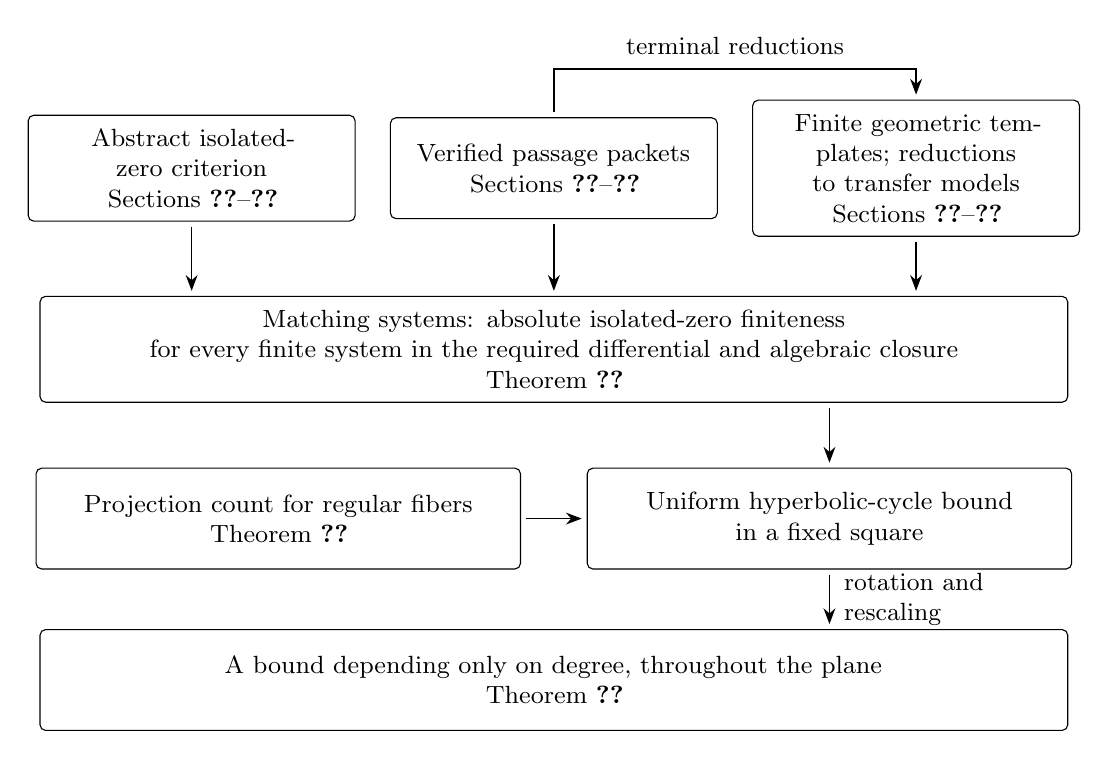
\begin{tikzpicture}[
  box/.style={draw,rounded corners=2pt,align=center,
    text width=3.8cm,minimum height=1.28cm,inner sep=5pt,
    font=\small},
  wide/.style={box,text width=12.7cm},
  half/.style={box,text width=5.8cm},
  flow/.style={-{Stealth[length=2mm]},semithick},
  every node/.style={outer sep=2pt}]
\node[box] (criterion) at (-4.6,0)
  {Abstract isolated-zero criterion\\
   Sections~\ref{sec:flags}--\ref{sec:elimination}};
\node[box] (packets) at (0,0)
  {Verified passage packets\\
   Sections~\ref{sec:additive}--\ref{sec:mixed}};
\node[box] (geometry) at (4.6,0)
  {Finite geometric templates; reductions to transfer models\\
   Sections~\ref{sec:subdivision}--\ref{sec:terminal}};
\node[wide] (matching) at (0,-2.3)
  {Matching systems: absolute isolated-zero finiteness\\
   for every finite system in the required differential and algebraic closure\\
   Theorem~\ref{thm:matching-system}};
\node[half] (projection) at (-3.5,-4.45)
  {Projection count for regular fibers\\
   Theorem~\ref{thm:projection-count}};
\node[half] (hyperbolic) at (3.5,-4.45)
  {Uniform hyperbolic-cycle bound\\in a fixed square};
\node[wide] (cycles) at (0,-6.5)
  {A bound depending only on degree, throughout the plane\\
   Theorem~\ref{thm:uniform}};
\draw[flow] (packets.north) -- ++(0,.55)
  -| node[pos=.25,above,font=\small] {terminal reductions} (geometry.north);
\draw[flow] (criterion.south)--(matching.north -| criterion.south);
\draw[flow] (packets)--(matching);
\draw[flow] (geometry.south)--(matching.north -| geometry.south);
\draw[flow] (matching.south -| hyperbolic.north)--(hyperbolic.north);
\draw[flow] (projection)--(hyperbolic);
\draw[flow] (hyperbolic.south)--
  node[right,align=left,font=\small] {rotation and\\rescaling}
  (cycles.north -| hyperbolic.south);
\end{tikzpicture}
\caption{Main theorem interfaces. Matching combines the finite geometric
 description with the packet criterion, retaining the exact graph ties
 and open domains. The independent projection theorem converts absolute
 finiteness for the full required closure into uniform component bounds.
 The sequence-dependent flags and internal factorizations used in the
 absolute-zero test do not enlarge the finite geometric alphabet.
 The packet input to Sections~\ref{sec:subdivision}--\ref{sec:terminal}
 concerns the terminal reductions, not the preparation of scalar fields.}
\label{fig:proof-map}
\end{figure}


The analytic flags and charts in an absolute-zero contradiction may
depend on the chosen sequence. They are not used as a finite covering
of coefficient space. The finite geometric description and the
projection-counting argument supply the uniformity.

For a first reading, the theorem statements cited above and the final
proof in Section~\ref{sec:counting} display the chain of implications.
Definition~\ref{def:counting-domain} specifies the precise closure
required at the counting interface. The preceding sections establish
its analytic and geometric inputs.

\subsection{Analytic ingredients}

Three features of the argument deserve emphasis.

A \emph{packet} records an actual analytic function together with two
trees of successive asymptotic expansions and the domain, transition,
and error estimates relating them. The two signs refer to lateral
determinations on either side of the real path; higher-band raw
realizations may be smooth interpolations of holomorphic determinations.

First, the separation theorem uses a \emph{tree} of expansions on
successive complex bands. It does not assume a simultaneous convergent
series in all small exponentials. The hypotheses record retained
arguments, permissible error costs, differentiated transition
estimates, and growth on the full fringes of the domains.
The proof upgrades arbitrarily high fixed exponential decay to exact
vanishing by weighted Cauchy corrections and maximum principles.
The domain and error conditions are indispensable: real asymptotic
flatness alone gives no such conclusion.

Second, regular ordinary implicit changes must be compatible with
dependent scales that can rotate rapidly under tiny complex
perturbations. The construction uses high real Taylor jets and
interpolation into small comparison tubes, with a fixed finite
coherence order at each stage. It does not require one ordinary
complex neighborhood valid for all derivative orders.
The later center-lifting argument additionally keeps the power
exponents controlling maps, inverses, and neighborhoods fixed while
the accuracy of auxiliary records is increased. This quantitative
property permits exact correction of approximate chart hits.

Third, the projection argument is formulated for an analytic class
closed under the particular derivatives, graph variables, and
multiplier equations used in its proof. Proper barriers and a fixed
generic tilt reduce the number of parameters. The resulting
absolute-to-uniform implication is independent of the particular
planar passage models and can be applied to other classes for which
the same hypotheses are established.

\subsection{Notation and conventions}

The technical constructions are local at a limiting ordinary analytic
germ. An asymptotic assertion is made for a fixed finite request:
a finite collection of expressions, derivative orders, Taylor
accuracies, and transition estimates. Constants, sufficiently far
starting points, and smaller neighborhoods may depend on that
request. Whenever an exponent must be independent of a later
accuracy choice, this is stated explicitly.

The notation used throughout the analytic part is summarized below;
see Definitions~\ref{def:flags-flag} and~\ref{def:packet}.
Local clock and state variables are introduced separately in each
passage model.

\begin{center}
\begin{tabular}{@{}ll@{}}
\toprule
Notation & Meaning\\
\midrule
\(Z_1\gg\cdots\gg Z_m\gg1\) & Ordered scales of a finite flag\\
\(f_i=\log Z_i,\quad h_i=e^{-Z_i}\) & Logarithmic scales and small exponentials\\
\(S\) & Tuple of independent, or free, flag scales\\
\(t,t_c\) & Ordinary inputs and their interior limiting germ point\\
\(b_i\) & Bounded ordinary backgrounds in exact log relations\\
\(\sigma(i)\) & Leading later index in a dependent log relation\\
\(s=u+iv\) & Complex parameter of a selected flag path\\
\(\Lambda_i=f_i'\) & Logarithmic rate along the real path\\
\(V_i=e^{f_i}/\Lambda_i\) & Precision scale at level \(i\)\\
\(S^{j,\pm}_\alpha\) & Raw packet in band \(j\) at prefix \(\alpha\)\\
\(h^\nu=\exp(-\sum_i\nu_iZ_i)\) & Exponential shift with lexicographic order\\
\bottomrule
\end{tabular}
\end{center}

Lexicographic order starts at the largest scale. A positive exponent
vector has positive first nonzero coordinate; later coordinates need
not be nonnegative. A vanishing coefficient means a vanishing
ordinary analytic germ. Complex logarithms and powers always use the
specified lifted determinations. A dependent scale is evaluated at
its \emph{current} background values, including after an implicit
change of ordinary variables.

All differentiations of primitive packets are in their independent
arguments. Equations tying those arguments are imposed only
afterward; differentiation of the resulting physical maps uses the
chain rule on the tied graph. This distinction is used repeatedly in
the terminal reductions and the matching equations.

\section{Finite logarithmic flags and angular paths}\label{sec:flags}

An unbounded sequence of equation arguments can involve several widely
separated scales. This section records those scales and their exact
logarithmic relations in a finite flag, then constructs complex paths
through the sequence anchors. Along these paths, the largest scale
approaches a vertical complex direction before the smaller scales do.
We construct nested contours on which their real parts remain positive
and quantitatively separated. These are the domains for the separation
argument in Section~\ref{sec:separation}. The final two lemmas control
anchor-dependent growth and simultaneous avoidance of finitely many
lattices of poles.


\subsection{Sequence conventions and exact logarithmic relations}

All constructions in this section concern a selected sequence of real
points. Passing to a subsequence is allowed. For positive quantities,
$X\gg Y$ means $X/Y\to+\infty$. A comparison involving finitely many
quantities, and comparisons of a finite list at every fixed iterated
exponential height, can be decided after a diagonal subsequence. None of
the resulting numbers of scales or heights is asserted to be uniform
over the original sequences.

The \emph{ordinary variables} have a finite limit $t_c$ in the interior of
an analytic argument neighborhood. Bounded ratios that a formula needs
are included among these arguments. Neighborhoods can be shrunk for
each finite request. The endpoint inequalities defining the actual
problem can nevertheless approach their boundary. An ordinary
coefficient equal to zero below means the zero analytic germ at $t_c$,
and not merely a function vanishing on the selected sequence.

\begin{definition}[Logarithmic flag]\label{def:flags-flag}
A logarithmic flag consists of positive scales
\[
 Z_1\gg Z_2\gg\cdots\gg Z_m\gg1,
 \qquad f_i=\log Z_i,\qquad h_i=e^{-Z_i},
\]
each declared either free or dependent. The tuple of free scales is
denoted by $S$. A dependent scale has the exact relation
\begin{equation}\label{eq:flags-triangular}
 f_i=\sum_{j>i}a_{ij}Z_j+b_i,
 \qquad
 \sigma(i)=\min\{j:a_{ij}\ne0\},\qquad a_{i,\sigma(i)}>0.
\end{equation}
The coefficients $a_{ij}$ are fixed real numbers, and the backgrounds
$b_i$ are bounded ordinary coordinates, or their current values on an
ordinary chart. The free scales are independent arguments; dependent
scales are always evaluated by Equation~\eqref{eq:flags-triangular}.

The saturation condition below will ensure that bounded changes of the
backgrounds preserve the ordered hierarchy. Two scales belong to the same
\emph{height block} if each is eventually
bounded by a finite iterated exponential of the other. A flag is
\emph{saturated} if, in every block containing a dependent node, all
dependent nodes precede all free nodes and
\begin{equation}\label{eq:flags-saturated}
 \log Z_{\text{first free}}=o\bigl(\log Z_{\text{last dependent}}\bigr).
\end{equation}
An all-free block has no additional condition.
\end{definition}

The relation defining height blocks is an equivalence relation: a
composition of finitely many iterated exponentials is another finite
iterate, after increasing the iterate to absorb fixed constants. Its
classes are consecutive in the ordering of the scales. A dependent
node and its leading child $\sigma(i)$ are in the same block, because
\[
 f_i=a_{i,\sigma(i)}Z_{\sigma(i)}(1+o(1)).
\]
In particular a dependency chain ends at a free node in the same block.

We use lifted logarithms and powers in complex continuations. Thus
$f_i$ continues as the expression in
Equation~\eqref{eq:flags-triangular}, even if $Z_i=e^{f_i}$ winds in
the plane. An exponential monomial is
\[
 h^\nu=\exp\Bigl(-\sum_{i=1}^m\nu_i Z_i\Bigr).
\]
Its order is the sign of the first nonzero entry of $\nu$, with the
largest scale first. This convention does not refer to the numerical
sign of the monomial. Known signs and ordinary units can be kept as
separate factors. Later expansions will be trees indexed by successive
prefixes of $\nu$; no simultaneous convergence of all these monomials
is implicit in this notation.

Inserting logarithms expresses fixed real powers of large inputs as
exponential monomials times bounded nonvanishing ordinary analytic factors. A later insertion of $-\log|t|$, when an ordinary
coordinate $t$ tends to zero, must also preserve the large coordinates
already free at that stage. The next lemma supplies these operations.

\begin{lemma}[Finite saturation and preservation of free coordinates]
\label{lem:flags-saturation}
A finite collection of large real inputs admits a flag after a fixed
linear change of coordinates and the addition of bounded ordinary
coordinates. One can insert the logarithm of any free scale, retaining
the old scale values, by making that scale dependent and adding at most
one positive free residual or one bounded ordinary residual. The free
residual is $O(\log S)$ if the scale being converted is $S$.

A flag admits a finite saturation by such insertions. After saturation,
promoting one ordinary coordinate $t\to0$ of known sign, by inserting
$-\log|t|$, admits a finite further saturation in which every old free
coordinate stays free. The number of ordinary coordinates does not
increase in this promotion.

\end{lemma}

\begin{proof}
For the initial linear reduction, choose a largest absolute value
among a basis of the finite span of the inputs. After a subsequence,
the ratios of the other elements to it have finite limits. Subtract
these limiting multiples. In the remaining span repeat the operation,
changing the sign of an unbounded residual when necessary. At each
step the dimension of the remaining span drops. A bounded residual is
retained as an ordinary coordinate, even if its selected values vanish; every unbounded residual chosen as a new scale
is strictly smaller than its predecessor. This gives a finite ordered
scale basis with constant coefficients.

Apply the same elimination to $\log S$ against the existing scale
basis, beginning with the largest scale. A scale much larger than
$\log S$ has zero coefficient. After subtracting its limiting multiple
at each comparable scale, the remainder is either bounded or, after
changing sign, a new positive scale separated from every old scale.
All the subtracted terms and the remainder are $O(\log S)$. Hence only
one new residual is needed. Since $\log S=o(S)$, its expression uses
only scales below $S$; it is therefore a relation of the form
Equation~\eqref{eq:flags-triangular}. Its first nonzero coefficient is
positive, since $\log S\to+\infty$. The old scale values have not been
changed.

Process the blocks containing dependent nodes from largest to
smallest. On entering a block fix its then smallest scale $T$.
Convert every free scale $R$ in that block for which
$\log R\ne o(\log T)$, and repeat this test only on any new residual
still in the block. Every continuing chain satisfies
\begin{equation}\label{eq:flags-residual-chain}
 R_{q+1}\le C_q\log R_q.
\end{equation}
The initial node of a chain is bounded by $\exp^{N}(T)$ for a fixed
$N$, by the definition of the block. Finitely many applications of
Equation~\eqref{eq:flags-residual-chain} give a residual $O(T)$ and
then one $O(\log T)$. The logarithm of the latter is
$o(\log T)$, so it is no longer converted. Fixed constants can be
absorbed by an extra logarithmic step. A residual that has entered a
lower block has already left the chain under consideration. There are
finitely many initial chains and each step has at most one child;
thus the procedure is finite. Residuals entering lower blocks are
free until that block is processed.

Every converted node in the block has, after the comparison
subsequence, $\log R\ge c\log T$. Every free node left at the end
has $\log F=o(\log T)$. The original dependent nodes also have
logarithms at least $\log T$. Consequently all dependent nodes
precede all remaining free nodes, and
Equation~\eqref{eq:flags-saturated} holds. All-free blocks need no
processing.

For a later promotion first insert $-\log|t|$ by the same linear
elimination. In each old block with dependent nodes keep the old cut
\[
 L=\log Z_{\text{old last dependent}}.
\]
Only the new residual chain is tested for conversion, with criterion
$\log R\ne o(L)$. For every old free node $F$,
$\log F=o(L)$. For each newly converted node $R$, the comparison
subsequence gives $\log R\ge cL$; therefore
\begin{equation}\label{eq:flags-old-free}
 \frac{\log F}{\log R}\longrightarrow0,
 \qquad \frac{R}{F}\longrightarrow+\infty.
\end{equation}
In particular a new residual below an old free node is never converted
in this block. Thus no old free coordinate is consumed, and the new
last-dependent cut still dominates the logarithms of all old free
nodes. The residual-chain argument proves termination here as well.
If the chain enters an old all-free block, leaving its residual free
introduces no dependent node into that block. Inserting new scales
cannot join two distinct old blocks: transitivity of finite-height
comparability would already have put their old members in one block.
The coordinate $t$ has been consumed; at most the final step of its
single chain produces a bounded residual. This proves the assertion
about the number of ordinary coordinates. The inverse expression for
$t$ has the form
\[
 t=\sgn(t)\exp\Bigl(-\sum_i\nu_iZ_i-B\Bigr),
\]
with $B$ bounded and with a positive first nonzero large coefficient
when such a coefficient occurs.

\end{proof}

The flag is now fixed. The next assertion concerns a different operation:
we hold its free inputs fixed and vary its bounded backgrounds, always
reevaluating dependent scales by their exact relations. This stability
will be needed when ordinary variables are changed implicitly.

\begin{lemma}[Stability under bounded backgrounds]
\label{lem:flags-stability}
On a saturated output flag of Lemma~\ref{lem:flags-saturation}, bounded
variations of the backgrounds at fixed free coordinates preserve the ordered scale hierarchy,
uniformly on each fixed bounded admissible real background set. More
precisely, let
\[
 H=\sum_{i=1}^m c_iZ_i+B,
\]
where the $c_i$ are fixed real numbers, their vector is nonzero,
and $B$ is uniformly bounded on that background set. If $k$ is the
first index with $c_k\ne0$, then
\[
 \frac{H}{c_kZ_k}\longrightarrow1
\]
uniformly under those variations; the denominator uses the current,
reevaluated value of $Z_k$. Thus the leading index and sign are
preserved. Dependent logarithms may enter such a comparison after
substitution of their exact triangular formulas. No sign assertion
is made when the resulting large part vanishes, or for an expression
containing an uninserted free logarithm.
\end{lemma}

\begin{proof}
Process the saturated output flag's height blocks from smallest to
largest. Each evaluated lower block is bounded above, uniformly on the fixed bounded real background set,
by a fixed finite exponential iterate of its largest free member.
Indeed it contains only finitely many triangular relations, whose
coefficients are fixed and whose backgrounds are bounded. Every free
member of a higher block dominates every such fixed iterate. Thus
lower-block values remain negligible compared with every free member
of the block being processed.

The free members of the current block are unchanged and ordered. If
the block has dependent members, let $d$ be its last one and put
$k=\sigma(d)$. The leading child lies in the same block and, by
saturation, is free. Its value is therefore unchanged. All later
scales have already been ordered, so the triangular relation gives
\[
 f_d=a_{dk}Z_k(1+o(1))
\]
uniformly on the background set. The logarithm of the first free
member is $o(f_d)$ on the original sequence. It remains so uniformly,
since that logarithm and $Z_k$ are fixed. This proves the
last-dependent/first-free boundary.

Now proceed upwards through the dependent members. The difference
of two consecutive dependent log relations is a fixed affine
combination of later scales and a bounded remainder. Its large part
is nonzero, since otherwise their logarithmic gap on the original
sequence would be bounded. Its first nonzero coefficient is positive
on that sequence. The later scales are already ordered uniformly by
the induction, so this coefficient still dominates. This proves all
remaining gaps and hence the full hierarchy uniformly.

Finally divide $H$ by $c_kZ_k$, evaluated at the current backgrounds.
Every later-scale ratio tends uniformly to zero, as does the bounded
remainder divided by $Z_k$. This proves the precise assertion about
affine comparisons. A combination involving dependent logarithms
first reduces to this form by exact substitution. If all large
coefficients cancel, their cancellation is an identity of fixed
coefficient vectors, leaving the current bounded remainder; it
supplies no additional sign conclusion.
\end{proof}

\subsection{Paths through far anchors}

We keep a saturated flag fixed and vary its free coordinates along a
complex path, with parameter $s=u+iv$. The path must pass through the
chosen anchor without
depending on the ordinary backgrounds, and it must preserve scale
separation on every required fixed backward interval. Its angular purpose
comes from the identity
\[
 \Re Z_i=e^{\Re f_i}\cos(\Im f_i).
\]
As $|v|$ grows, the larger scales must approach the directions
$\Im f_i=\pm\pi/2$ before the smaller ones. With
$\Lambda_i=f_i'$ on the real ray, the path estimates below give
$\Im f_i(u+iv)\sim v\Lambda_i(u)$: the level-$i$ direction is
therefore reached at distance about $\pi/(2\Lambda_i)$ from that
ray. We first construct the paths and estimate these logarithmic rates;
the next subsection chooses the precise contours and their margins.


Write $\operatorname{polylog}X$ for a bound
$C(1+\log X)^N$, where $C,N$ may change between occurrences and may
depend on a fixed derivative order. In every use the number of
derivatives and the other requests are finite. Thresholds, constants,
and ordinary neighborhoods may depend on this finite request.

Fix a far anchor, write its smallest logarithm as $f_m^0$, and put
$u_0=\log f_m^0$. We construct paths $s=u+iv$ through the free
coordinates, defined over $u\ge u_0-B$ for any required fixed
backstep $B$. All tuning constants are held fixed when testing a path.
The smallest node is necessarily free. Its path is
\[
 f_m(s)=e^s.
\]
Now take $i=m-1,\ldots,1$. Dependent nodes are evaluated from
Equation~\eqref{eq:flags-triangular}. At a free node $i<m$ set
$n=i+1$ and use the following rules.

If the successor $n$ is free, put $f_i=f_n+g_i$. A positive
logarithmic gap can usually be continued by
\begin{equation}\label{eq:flags-uncapped}
 g_i=x_i,\qquad x_i(s)=x_i^0 e^{s-u_0},
\end{equation}
with $x_i^0$ equal to the anchor gap. Within a block containing
dependent nodes, some free gaps must also stay small relative to the
leading child of the last dependent node. If that node is $d$ and
$k=\sigma(d)>i$, cap the gap by using
\begin{equation}\label{eq:flags-cap}
 g_i=\frac{x_i y_i}{x_i+y_i},\qquad
 y_i=\eta_i Z_k,
 \qquad
 x_i^0=\frac{g_i^0y_i^0}{y_i^0-g_i^0}.
\end{equation}
Here $k$ is free. Saturation gives $g_i^0=o(Z_k^0)$, so one can take
$\eta_i\to0$ so slowly that $g_i^0=o(y_i^0)$ and, for every
backstep needed in the finite request,
\begin{equation}\label{eq:flags-eta}
 \eta_i\ge Z_k(u_0-B)^{-1/4}.
\end{equation}
Then $x_i^0\sim g_i^0\to\infty$. The number $\eta_i$ is fixed
on the resulting path, though it tends to zero as anchors recede.

If the successor $n$ is dependent, saturation puts $i$ and $n$ in
different blocks. The new free path must dominate $f_n$ while remaining
independent of its backgrounds. For this purpose, follow leading children
from $n$ to its terminal free node
$k$, using $\ell$ edges, and put
\begin{equation}\label{eq:flags-boundary}
 T=\exp^{\ell-1}(Z_k^2),\qquad
 f_i=T^2+x_i,\qquad x_i=x_i^0e^{s-u_0}.
\end{equation}
The original distinct heights give $f_i^0\gg (T^0)^2$, so
$x_i^0=f_i^0-(T^0)^2>0$ and tends to infinity. Crucially, this rule
uses only the free node $k$, not an ordinary input or a dependent
value whose background could later change.

The real ordinary inputs can be constant, or can vary with bounded
derivatives of all the fixed orders used. Independent ordinary tests
are chosen real-symmetric and holomorphic, with positive-order
derivatives tending to zero, and return to $t_c$ as $u\to\infty$
on each individual path. For example, an anchor value $t^0$ in a
smaller convex box can be tested by
\[
 t(s)=t_c+(t^0-t_c)e^{-\delta(s-u_0)},
\]
with $\delta>0$ as small as needed and with slack for the fixed
backstep. This also shows why smaller ordinary boxes requested later
can be reached on the same ray. It is not necessary that all finite
requests hold at the anchor with one common threshold.

For complex estimates, a \emph{controlled background determination}
means a local continuation with uniform Taylor control on the angular
range in question. In particular it satisfies
\[
 b(u+iv)=b(u)+ivb'(u)+O(v^2),\qquad
 \partial_v b(u+iv)=ib'(u)+O(|v|),
\]
and the corresponding Taylor estimates through every fixed order
requested at that step. The real jets are bounded. Several piecewise
holomorphic determinations can have the same real jets; negligible
errors arising from their smooth interpolation are retained as defects
in the packet estimates below. Real boundedness alone is not used to
infer these complex bounds.

\begin{lemma}[Real and angular path estimates]\label{lem:flags-path}
The paths just constructed pass through the given anchors and
preserve the ordered scales under bounded controlled ordinary tests.
Put $\Lambda_i=f_i'$ on the real ray. For each $G=f_i-f_j$, $i<j$,
and for each fixed positive integer $r$, sufficiently far out,
\begin{equation}\label{eq:flags-real}
 \begin{gathered}
 G\longrightarrow+\infty,\qquad
 cG\le G'\le G\operatorname{polylog}G,\\
 |G^{(r)}|\le G\operatorname{polylog}G,\qquad
 0<\frac{(f_i-f_{i+1})'}{f_i-f_{i+1}}
       \le C\Lambda_{i+1}.
 \end{gathered}
\end{equation}
The first three bounds also hold with $G$ replaced by $f_i$.
In particular
\begin{equation}\label{eq:flags-rates}
 \Lambda_1>\cdots>\Lambda_m\longrightarrow+\infty,
 \qquad cf_i\le\Lambda_i\le f_i\operatorname{polylog}f_i,
 \qquad \frac{f_i''}{\Lambda_i^2}=o(1).
\end{equation}
Fixed backsteps can reduce $f_i$ by any prescribed fixed factor.

With holomorphic background tests, the formulas for indices $j\ge p$
have controlled holomorphic continuations on $|v|\le C/\Lambda_p(u)$
and satisfy
\begin{equation}\label{eq:flags-angular}
 \begin{aligned}
 \Re f_j(u+iv)&=f_j(u)+o(1),\\
 \Im f_j(u+iv)&=(1+o(1))v\Lambda_j(u),\\
 \Im(f_j-f_l)(u+iv)&=(1+o(1))v(\Lambda_j-\Lambda_l)(u),
                       && l>j,\\
 \partial_v\Im f_j(u+iv)&=(1+o(1))\Lambda_j(u).
 \end{aligned}
\end{equation}
These estimates also hold for controlled local determinations of the
backgrounds that agree with the real path to their requisite finite
Taylor orders; their antiholomorphic defects, if present, are accounted
for separately. For a retained free input $Z_l$, every fixed path
derivative is bounded by $\exp(C_r f_l(u))$ on its applicable angular
range.
\end{lemma}

\begin{proof}
We give the induction estimates, including the cases in which a
smaller scale can have a relatively large logarithmic derivative.
The initial function $f_m=e^u$ has all the required estimates.
If a positive function $F$ satisfies the first three real bounds,
the formula for a derivative of $e^F$ is $e^F$ times a polynomial in
$F',\ldots,F^{(r)}$. Consequently
\begin{equation}\label{eq:flags-exp-derivative}
 |(e^F)^{(r)}|\le e^F\operatorname{polylog}(e^F).
\end{equation}
Finite sums with a separated positive leading term obey the same
upper bounds. Their first derivative has that leading positive term:
the derivative ordering already known at later nodes and the
exponential modulus gaps make the lower terms negligible. This
handles dependent logs and differences of dependent logs. Fixed
bounded derivatives of the backgrounds are lower-order terms.

An uncapped gap has $x_i^{(r)}=x_i$ and poses no difficulty. For a
cap write $x=x_i$, $y=y_i$, $r_0=x/y$. Direct differentiation gives
\begin{equation}\label{eq:flags-cap-derivative}
 \frac{g'}g=\frac{1+r_0\Lambda_k}{1+r_0}.
\end{equation}
This is positive, bounded below by a fixed positive constant, and
bounded above by $1+\Lambda_k\le C\Lambda_n$. In addition,
Equation~\eqref{eq:flags-eta} gives
$\Lambda_k\le\operatorname{polylog}y$. If $x\le y$, then
$g\asymp x$, and the elementary bound
\[
 \frac{x}{y}(1+\log y)^N\le C_N(1+\log x)^N
 \quad(x\le y,\ x\hbox{ sufficiently large})
\]
absorbs each occurrence of a $y$ derivative. To verify the bound,
write $y=xe^a$ and use
$e^{-a}(1+\log x+a)^N\le C_N(1+\log x)^N$.
If $x\ge y$, then $g\asymp y$ and the bound is immediate.
Repeated differentiation of $xy/(x+y)$ gives the same alternatives:
terms containing a derivative of $y$, after division by $g$, have a
factor $O(x/y)$ when $x\le y$, and otherwise have only fixed powers
of logarithms of $y$. This proves the fixed-order bounds in $g$.

For the boundary rule, repeated use of the positive leading terms
on the chain from $n$ to $k$ gives, sufficiently far out,
\begin{equation}\label{eq:flags-height-offset}
 \exp^{\ell-1}(Z_k^{1/2})\le f_n
       \le \exp^{\ell-1}(Z_k^2)=T.
\end{equation}
Every fixed logarithmic derivative of $T$ is bounded by a power of
$1+\log T$. Its first logarithmic derivative is $o(f_n)$: for
$\ell=1$ this follows from
$T'/T=2\Lambda_k=o(Z_k^{1/2})$; for larger $\ell$, the numerator
is a product of lower iterates, whereas the left side of
Equation~\eqref{eq:flags-height-offset} has one more exponential
height. Thus $T^2+x_i$ and its first derivative dominate $f_n$ and
$f_n'$. The gap $T^2+x_i-f_n$ has the first three real estimates,
and
\[
 \frac{(T^2+x_i-f_n)'}{T^2+x_i-f_n}
 \le C\left(1+\frac{T'}T\right)\le C\Lambda_n.
\]
The same computations give its fixed-order bounds.

There remains the dependent-to-free boundary in a saturated block.
Let $d$ be its last dependent node and $k=\sigma(d)$. The only
free gaps above $k$ are the caps in
Equation~\eqref{eq:flags-cap}, so their finite sum is $o(Z_k)$ at
the anchors, with first derivative $o(Z_k\Lambda_k)$. For example,
Equation~\eqref{eq:flags-cap-derivative} and $g\le\eta_iZ_k$
bound the derivative by $C\eta_iZ_k(1+\Lambda_k)$.
On each individual forward ray, $x_i/Z_k\to0$, because $x_i$ grows
as $e^u$ and $f_k\ge e^u$ eventually. Hence the same little-oh
bounds hold towards infinity on that ray, with its tuning constants
fixed. The remaining free contribution is $f_k=o(Z_k)$, whose
first derivative is $o(Z_k\Lambda_k)$. Therefore
\[
 f_{d+1}=o(Z_k),\qquad
 f_{d+1}'=o(Z_k\Lambda_k),
\]
whereas $f_d\sim a_{dk}Z_k$ and
$f_d'\sim a_{dk}Z_k\Lambda_k$.
This proves the real estimates across this boundary, including
\[
 \frac{(f_d-f_{d+1})'}{f_d-f_{d+1}}
       \asymp\Lambda_k\le\Lambda_{d+1}.
\]
Higher derivatives of the caps are bounded by
$Z_k\operatorname{polylog}Z_k$, which suffices here. Between two
dependent nodes the leading scale of their difference has index at
least that of the leading scale in the earlier relation. Its
logarithmic derivative is at most $C\Lambda_{i+1}$: if its index
is $i+1$ this is immediate, and otherwise use the already proved
ordering of later derivatives. This completes the adjacent-gap
induction. A nonadjacent gap is a finite sum of adjacent positive
gaps, proving its first three estimates. The lower constant can,
for example, be taken to be $c=1/2$ after going sufficiently far
for any chosen fixed backstep: uncapped terms and caps have
logarithmic derivative at least one, and dependent leading terms
and the $T$ terms have logarithmic derivatives tending to infinity.
The discarded terms are relatively negligible. Thus a backstep
$B\ge2\log R$ reduces every $f_i$ by at least a prescribed factor
$R$, once that fixed backstep is included in the construction.

For completeness, the continuation uses the explicit formulas, not
an arbitrary holomorphic function having prescribed real bounds.
In the downward induction, a dependent $f_j$ is a finite affine sum
of $Z_k$ with $k>j$. The already controlled real parts of $f_k$
make $|Z_k(u+iv)|\asymp Z_k(u)$, so differentiating this sum
retains the bounds of Equation~\eqref{eq:flags-exp-derivative}.
The same argument applies directly to a dependent gap, using its
first surviving coefficient. In a boundary term $T$, every proper
exponent in its finite exponential tower and its fixed derivatives
are bounded by a power of $1+\log T$. Since
$|v|\le C/\Lambda_i\le C'/T^2$, their variations tend to zero.
Induction through that finite tower therefore preserves its moduli
and the derivative estimates. An uncapped additive term has its
explicit exponential continuation.
In a cap, if $|x|$ and $|y|$ are separated, $x+y$ stays away from
zero. If they are comparable, then $y=O(f_i)$ at the controlling
node, and
$|\arg y|=O(\Lambda_k/\Lambda_i)=o(1)$; indeed in this case
$\Lambda_i\ge cg\asymp y$, whereas
$\Lambda_k\le\operatorname{polylog}y$.
The denominator therefore again stays away from zero. These
observations prove by the same downward induction that the real
derivative bounds used above remain valid, with fixed enlarged
constants, along the short vertical segment.

Taylor's formula along that segment now gives
\[
 |\Re f_j(u+iv)-f_j(u)|
 \le C v^2 f_j(u)\operatorname{polylog}f_j(u)=o(1),
\]
since $\Lambda_p\ge cf_p\ge cf_j$. For a gap $G=f_j-f_l$
it gives an error bounded by
$Cv^2G\operatorname{polylog}G$. Dividing by
$|v|G'\ge c|v|G$ gives
$O(\operatorname{polylog}G/\Lambda_p)=o(1)$.
Applying this estimate directly to the gap, rather than subtracting
two relative estimates for individual logs, proves the third line
of Equation~\eqref{eq:flags-angular} even for nearly equal speeds.
The individual imaginary and derivative assertions follow in the
same way. Controlled backgrounds have the same Taylor bounds and
therefore give the stated version for local determinations. Finally,
the derivative polynomial for $Z_l=e^{f_l}$ is bounded by
$e^{f_l}\operatorname{polylog}(e^{f_l})\le e^{C_rf_l}$.
\end{proof}

\begin{remark}\label{rem:flags-path-heights}
Different original height blocks need not stay different along an
individual forward ray. The conclusions that persist are the ordered
scale ratios, the exact logarithmic relations, and
Equations~\eqref{eq:flags-real}--\eqref{eq:flags-angular}. These
are the conclusions used below. The paths of free inputs were defined
without ordinary backgrounds, which permits independent ordinary
tests and later regular implicit substitutions.
All comparisons defining a fixed finite real regime have slack
sufficiently far along the selected sequence. Continuity of the
finite triangular formulas therefore permits sufficiently small
absolute perturbations of the free inputs while retaining that
regime and the limiting ordinary data. Their permitted sizes may
depend on the anchor; no fixed neighborhood is intended.
\end{remark}

\subsection{Nested contours and background variation}

At level $p$ we use two boundaries before $Z_p$ reaches a vertical
direction. A good contour leaves $\Re Z_p$ of order
$V_p=e^{f_p}/\Lambda_p$, large enough to dominate the later real
parts. The outer side is closer to vertical; its defining barrier
retains both that domination and an explicit polynomial angular margin.
These margins also determine how accurately two background determinations
must agree.

\begin{lemma}[Good contours and buffered sides]\label{lem:flags-contours}
For a sufficiently small fixed $\eps>0$, the upper and lower
$p$-good contours are defined by
\begin{equation}\label{eq:flags-good}
 |\Im f_p|\sim\frac\pi2,\qquad
 \cos(\Im f_p)=\frac{\eps}{\Lambda_p(u)}.
\end{equation}
They have collars of fixed small multiples of their cosine margin
and are nested in increasing order of $p$. Put
\[
 V_p(u)=\frac{e^{f_p(u)}}{\Lambda_p(u)}.
\]
On a $p$-good contour, for $j>p$ and $G=f_p-f_j$,
\begin{equation}\label{eq:flags-good-real}
 \Re Z_p\sim\eps V_p,
 \qquad
 \Re Z_j\asymp
 \frac{e^{f_j(u)}(\eps+G'(u))}{\Lambda_p(u)}
       =o(V_p).
\end{equation}

For large fixed $A$ and fixed $K\ge2$, an outer side can be placed
inside the signed vertical direction by the barrier
\begin{equation}\label{eq:flags-side}
 L_p=Z_p-A\sum_{j>p}Z_j-\frac{Z_p}{f_p^K},
 \qquad \Re L_p=0.
\end{equation}
We use its inward component, where $\Re L_p>0$. Throughout this
component, with harmless fixed adjustments near its boundary,
\begin{equation}\label{eq:flags-buffer}
 \Re Z_p\ge A\sum_{j>p}\Re Z_j
               +c\frac{e^{f_p(u)}}{f_p(u)^{K+1}},
 \qquad \Re Z_p\gg f_p(u)^N
 \quad\hbox{for every fixed }N.
\end{equation}
The side and good contours can be chosen with extra room before any
finite subsequent narrowing. The same conclusions hold if the
quantities in the barrier are replaced by holomorphic proxies with
absolute $o(1)$ errors.

Uniformly between the $p$-good contour and its outer side, for
$p<n<l$,
\begin{equation}\label{eq:flags-later-real}
 \Re Z_l=o(\Re Z_n).
\end{equation}
Every retained index $j\ge p$ has a polynomial buffer of its own:
for some fixed exponent $C$,
\begin{equation}\label{eq:flags-retained-buffer}
 \Re Z_j\ge\frac{e^{f_j(u)}}{(1+f_j(u))^C}.
\end{equation}
In particular $\Re Z_j/f_l(u)\to\infty$ for $l\ge j$, so
fixed derivative losses $\exp(C'f_l)$ can be absorbed by any fixed
positive exponential decay in $\Re Z_j$.
\end{lemma}

\begin{proof}
By Equation~\eqref{eq:flags-angular}, $\Im f_p$, the lifted phase
of $Z_p$, is strictly increasing with $v$ near the positive
vertical position of $Z_p$,
which is at $v=(1+o(1))\pi/(2\Lambda_p)$. This gives the upper
contour, and real symmetry gives the lower one. If $j>p$, the
relative gap formula, with
$\eta_p=\cos(\Im f_p)\ge0$, gives
\begin{equation}\label{eq:flags-cosine}
 \Re Z_j\asymp e^{f_j(u)}
   \left(\eta_p+
               \frac{\Lambda_p-\Lambda_j}{\Lambda_p}\right)
\end{equation}
near the vertical direction. This also holds with the evident
constant-factor interpretation when the ratio of speeds is bounded
away from one. On a good contour it proves
Equation~\eqref{eq:flags-good-real}, since
$e^{-G}(\eps+G')\to0$ by the polylogarithmic upper bound for
$G'$. Moreover $G'\to\infty$, so the later phase is farther from
vertical than any fixed-width $p$ collar. This proves nesting even
when the two speeds have ratio tending to one. Farther inside, all
relevant cosines are bounded below, and the same ordering is simpler.

To compute the buffer, write $f_p=a+i\theta$, with
$a=f_p(u)+o(1)$ and $|\theta|\le\pi/2$. Uniformly near the upper
vertical direction,
\begin{equation}\label{eq:flags-buffer-expansion}
 \Re\frac{Z_p}{f_p^K}
 =e^a a^{-K}\left(
   \cos\theta+\frac{K\theta}{a}\sin\theta+O(a^{-2})\right).
\end{equation}
The second term is positive and of size $1/a$ near vertical.
The lower direction gives the same sign, since
$\theta\sin\theta>0$. Away from vertical, the first term gives
an even larger lower bound. Thus the real part in
Equation~\eqref{eq:flags-buffer-expansion} is at least
$ce^a/a^{K+1}$ throughout the required wedge.
At the good contour this term and the later real phases are
$o(\Re Z_p)$, so $\Re L_p>0$ there. At the exact vertical
direction $\Re Z_p=0$ and both subtracted real terms are positive.
The inward component therefore meets a zero side before vertical,
and positivity of its barrier gives
Equation~\eqref{eq:flags-buffer}. More explicitly, division of the
side equation by $e^{f_p(u)}$, followed by
Equation~\eqref{eq:flags-cosine}, gives, with $F=f_p(u)$,
\[
 \eta_{p,\mathrm{side}}\asymp F^{-K-1}
   +A\sum_{j>p}e^{-(f_p-f_j)}
                    \frac{\Lambda_p-\Lambda_j}{\Lambda_p}.
\]
The terms proportional to $\eta_{p,\mathrm{side}}$ on the
right have coefficient tending to zero and were absorbed on the
left. Hence $\Lambda_p\eta_{p,\mathrm{side}}\to0$, by the
polylogarithmic gap estimates. The side therefore lies beyond
every fixed good contour and still before the vertical direction.
This argument uses no global
injectivity of $Z_p$ or of a proxy. An initial choice with smaller
$A$ and larger $K$ supplies extra room; increasing $A$ and slightly
decreasing $K$ afterwards moves the working side inward. Absolute
$o(1)$ corrections are negligible compared with its diverging
buffer. The identical sign argument constructs the corrected side
within that extra room.

For the relative statement let $H=f_n-f_l$. From
Equation~\eqref{eq:flags-cosine},
\[
 \frac{\Re Z_l}{\Re Z_n}
 \le C e^{-H}\left(
  1+\frac{\Lambda_n-\Lambda_l}
  {\Lambda_p\eta_p+\Lambda_p-\Lambda_n}\right).
\]
The denominator is at least
$(f_p-f_n)'\to\infty$, whereas
$\Lambda_n-\Lambda_l\le H\operatorname{polylog}H$.
The right side tends to zero uniformly, proving
Equation~\eqref{eq:flags-later-real}. This is why one fixed
increase of $A$ can pay any prescribed finite collection of later
phase losses at the current side.

Finally consider $j>p$. If
$\Lambda_j\le\Lambda_p/2$, Equation~\eqref{eq:flags-cosine}
gives a fixed positive cosine for $Z_j$. Otherwise
$\Lambda_p\le2\Lambda_j$, and
\[
 f_p\le C\Lambda_p\le C f_j\operatorname{polylog}f_j.
\]
The polynomial angular margin supplied by
Equation~\eqref{eq:flags-buffer} for $p$ is therefore also an
inverse power of $f_j$. Equation~\eqref{eq:flags-cosine} again
proves Equation~\eqref{eq:flags-retained-buffer}. The case $j=p$
is already Equation~\eqref{eq:flags-buffer}.
\end{proof}

We next compare the domains obtained from different determinations of
the same real backgrounds. At a level-$p$ contour, first-jet agreement
preserves the separation of later phases from the vertical direction.
Locating the perturbed determination's own thin side requires higher,
but still finite, agreement.

\begin{lemma}[Sensitivity to background jets]\label{lem:flags-background}
Let $q\ge2$ be a fixed integer. On
$|v|\le C/\Lambda_p(u)$, two controlled background
determinations differing by $O(|v|^q)$, and agreeing on the real
path, change any $f_l$, $l\ge p$, by
\begin{equation}\label{eq:flags-background}
 |\Delta f_l|\le C\Lambda_l(u)|v|^q.
\end{equation}
The estimate is uniform along the short segment between the two
determinations when that segment is taken with the same background
slack. In particular agreement through the real first jet gives
$O(\Lambda_l v^2)$. On the angular scale $|v|=O(1/\Lambda_p)$
this error is smaller than the phase gain $(\Lambda_p-\Lambda_l)/\Lambda_p$ for $l>p$.
Agreement through a sufficiently high fixed jet preserves any
prescribed polynomial angular buffer and good-contour collar.
\end{lemma}

\begin{proof}
A free log has zero background sensitivity. For a dependent node,
differentiate Equation~\eqref{eq:flags-triangular}. By downward
induction and the leading positive derivative estimate,
\[
 \sum_{k\ge\sigma(l)}Z_k(u)(1+\Lambda_k(u))
       \le C\Lambda_l(u).
\]
Exponential moduli remain comparable on the stated angular scale.
The derivative of $f_l$ with respect to each bounded background is
therefore at most $C\Lambda_l(u)$. Integrating this derivative
between the two determinations proves
Equation~\eqref{eq:flags-background}; it also proves inductively
that the intermediate determinations remain in the allowed range.
For $q=2$ the error is at most $C/\Lambda_p$, while
$(\Lambda_p-\Lambda_l)/\Lambda_p\gg1/\Lambda_p$ by
Equation~\eqref{eq:flags-real}. For an own-contour comparison,
$\Lambda_p|v|^q=O(\Lambda_p^{1-q})$. The two-sided polynomial
bounds for $\Lambda_p$ in $f_p$ imply that choosing a fixed $q$
large enough makes this smaller than each of the finitely many
specified polynomial margins. No infinite-order jet matching is
being asserted.
\end{proof}

When backgrounds have slightly different band determinations, the
first-jet comparison in Lemma~\ref{lem:flags-background} suffices
for later phase comparisons: its $O(1/\Lambda_p)$ angular error
is swallowed by the diverging gap derivative. Locating a
determination's own thin side or its own good collar by a common
reference uses the higher finite jet comparison instead. This
distinction will be retained in ordinary implicit substitutions.

\subsection{Exceptional growth and safe columns}

An uncapped summand can make $\log(2+\Lambda_p)$ too large to
absorb in $\Re Z_{p+1}$. The constant $D_p$ below records the
remaining anchor dependence. The second lemma selects vertical columns
that avoid finitely many real pole lattices; when $D_p$ is large, it
also preserves this avoidance throughout the collar windows needed in
separation. All these assertions concern a fixed finite request.

\begin{lemma}[The exceptional anchor constant]\label{lem:flags-exceptional}
For $p<m$ set $D_p=\log(2+x_p^0)$ if $f_p$ contains an
uncapped slow additive term in
Equation~\eqref{eq:flags-uncapped} or
Equation~\eqref{eq:flags-boundary}, and set $D_p=1$ otherwise.
Set $D_0=1$. On the buffered level-$n$ wedge, $n=p+1$,
\begin{equation}\label{eq:flags-D}
 \log(2+\Lambda_p)\le C D_p+o(\Re Z_n).
\end{equation}
If $D_p$ is large, then throughout the fixed-backstep range
\begin{equation}\label{eq:flags-D-speed}
 \Lambda_p(u)\ge c_B e^{D_p}e^{u-u_0}.
\end{equation}
\end{lemma}

\begin{proof}
If $p$ is dependent, $f_p=O(Z_n)$ and
$\Lambda_p\le Z_n\operatorname{polylog}Z_n$ by its triangular
relation. Thus $\log(2+\Lambda_p)=O(f_n+\log f_n)$, which is
$o(\Re Z_n)$ by the polynomial buffer. A cap has size at most
a later scale and its logarithmic derivative is bounded by a
polylogarithm of that scale, giving the same conclusion. In the
boundary construction, the height offset gives
\[
 \log T=o\left(\frac{Z_n}{f_n^N}\right)
 \quad\hbox{for every fixed }N;
\]
this follows directly from
Equation~\eqref{eq:flags-height-offset}, since one additional
exponential dominates all its fixed powers. It bounds the
$T$ contribution to $\log(2+\Lambda_p)$. The only remaining
contribution is
\[
 \log(2+x_p(u))\le D_p+O(1+|u-u_0|).
\]
The second term is $o(\Re Z_n)$ on the forward ray and on each
fixed backstep, because $f_n\ge f_m=e^u$ and the buffer grows
exponentially in $f_n$. This proves
Equation~\eqref{eq:flags-D}. An uncapped term contributes exactly
$x_p^0e^{u-u_0}$ to the positive derivative of $f_p$; its other
terms have positive derivatives. For large $D_p$,
$x_p^0\asymp e^{D_p}$, proving
Equation~\eqref{eq:flags-D-speed}.
\end{proof}

The following elementary consequence is recorded for use when raw
coefficients have poles at finitely many real lattices. It asserts
safety for each finite request, not for an infinite set of labels.

\begin{lemma}[Common safe columns]\label{lem:flags-safe-columns}
Let a fixed finite list of positive real sweeps $x_a(u)$ and real
lattices $c_a+h_a\ZZ$, $h_a>0$, satisfy, uniformly far out,
\begin{equation}\label{eq:flags-sweeps}
 \begin{gathered}
 x_a\to\infty,\qquad x_a'>0,\qquad
 \inf_{u\ge U}x_a'(u)\longrightarrow\infty\quad(U\to\infty),\\
 \left|\frac{x_a''}{(x_a')^2}\right|\le\frac{C_a}{x_a}.
 \end{gathered}
\end{equation}
For a sufficiently small fixed $\delta>0$, every fixed-length
real interval far out contains a common column $u_*$ with
\[
 \dist(x_a(u_*),c_a+h_a\ZZ)\ge2\delta
 \quad\hbox{for all }a.
\]
If their complex continuations obey
\[
 |\Im x_a(u_*+iv)|<1
 \quad\Longrightarrow\quad
 |\Re x_a(u_*+iv)-x_a(u_*)|=o(1),
\]
these columns stay a fixed positive distance from all the listed
real poles on their whole applicable angular ranges.

Suppose additionally that on a band $j=p+1$ the relevant sweeps
satisfy $x_a'=O(Z_j\Lambda_j)$ and that at the chosen column
\begin{equation}\label{eq:flags-D-active}
 D_p>\frac{Z_j(u_*)}{f_j(u_*)^{K+3}}.
\end{equation}
Then safety persists throughout every required fixed collar window
\[
 |f_p(u)-f_p(u_*)|\le C_1\log(2+D_p)
\]
in the fixed-backstep range.
\end{lemma}

\begin{proof}
For one sweep use $x=x_a$ as a coordinate and let
$w(x)=1/x_a'(u(x))$. Then
\[
 \frac{\dd}{\dd x}\log w(x)
       =-\frac{x_a''}{(x_a')^2}=O(1/x).
\]
On any fixed lattice period the ratio of the largest and smallest
values of $w$ tends to one. The time spent within distance
$2\delta$ of its lattice is consequently at most
$C_a'\delta/h_a$ times the period's total time. Sum over the
complete periods of a fixed $u$-interval. At most two incomplete
end periods remain; their total time tends to zero by the lower
bound on $x_a'$. Thus the bad proportion for this sweep is at most
$C_a'\delta/h_a+o(1)$. A union bound over the finite list makes
the common bad proportion less than one, by first choosing
$\delta$ sufficiently small. This does not require independent
or incommensurable sweeps. If the complex imaginary part has
absolute value at least one, it already separates the point from
the real lattice. Otherwise the assumed real shift is $o(1)$,
which preserves the original detuning with slack.

Under Equation~\eqref{eq:flags-D-active},
\[
 \log(Z_j\Lambda_j)=O(f_j+\log f_j)=o(D_p).
\]
Equation~\eqref{eq:flags-D-speed} makes the stated $f_p$ window
have real width $O(e^{-D_p}\log(2+D_p))$. On this window the
real derivative bounds ensure the same local estimates for
$Z_j\Lambda_j$; for example its logarithmic derivative has
size at most $\operatorname{polylog}Z_j=\exp(o(D_p))$ and
therefore changes its logarithm by $o(1)$. Each sweep changes by
at most
\[
 e^{-D_p+o(D_p)}\log(2+D_p)=o(1).
\]
The detuning again persists with slack. This proves the collar
assertion.
\end{proof}

\section{Separation of packets}\label{sec:separation}


We expand an analytic function successively along a tree: each
coefficient at one level is expanded again at the next.  No convergence
of a series in all the quantities
$h_i=\exp(-Z_i)$ is asserted or used.  The distinction is particularly
important when a coefficient has zero formal data: decay to every fixed
order at its own level must first be strengthened before that coefficient
can be passed at the preceding level.

Uniqueness of an analytic function from its complete asymptotic data
belongs to the quasianalytic approach developed in the
limit-cycle literature \citep{Ilyashenko1991,Ecalle1992}.
Transserial Ilyashenko algebras provide a related injectivity theorem
for their own expansion classes \citep{GalalKaiserSpeissegger2020}.
Here the hypotheses are the precise band, transition, and source
estimates below, and the proof establishes the needed implication
directly for those data.

\subsection{Data and quantifiers}

Fix a saturated flag and the paths of Lemma~\ref{lem:flags-path}.
We use $s=u+iv$, $f_i=\log Z_i$, $\Lambda_i=f_i'$ on the real
path, and
\[
 V_i(u)=\frac{e^{f_i(u)}}{\Lambda_i(u)}.
\]
All logarithms have their lifted determinations.  The symbol $b_j$
below denotes the entire vector of bounded backgrounds in band $j$;
its components enter the triangular flag equations.  Accordingly,
$f_{k,j}$ and $Z_{k,j}$ denote the $k$th logarithm and scale evaluated with
that vector.  The subscripts on $b_j$ do not denote the index of an
individual triangular equation.

A \emph{good contour of level $i$} means either of the contours
of Lemma~\ref{lem:flags-contours} with
\begin{equation}\label{eq:separation-good}
 \cos(\Im f_i)=\frac{\epsilon_i}{\Lambda_i},\qquad
 V_i=\frac{e^{f_i}}{\Lambda_i},
\end{equation}
where $\epsilon_i>0$ is fixed and can be chosen arbitrarily small.
Contours always have small collars.  A \emph{side of level $i$}
is the boundary of the positive-real-part region of a holomorphic
proxy for
\begin{equation}\label{eq:separation-barrier}
 L_i=Z_i-A\sum_{k>i}Z_k-\frac{Z_i}{f_i^K}.
\end{equation}
Here $A$ is sufficiently large for the finite calculation under
consideration, and $K$ lies in a fixed interval with room to decrease
it finitely, for example $2\leq K\leq4$.  Proxy construction is proved
below.  Before constructing the proxy, the domain has extra angular
room.  A later increase of $A$ and decrease of $K$ puts the final side
strictly within that room.

The exceptional constants $D_i$ are those of
Lemma~\ref{lem:flags-exceptional}: $D_i=\log(2+x_0)$ when $f_i$
contains an uncapped slow summand with coefficient $x_0$, and $D_i=1$
otherwise; put $D_0=1$.  These constants remain fixed on each chosen
path.  They need not remain bounded as its anchor tends to infinity.

\begin{definition}[Packet data]\label{def:packet}
Let $t_c$ be a real ordinary germ point.  A packet consists of the
following data and estimates, separately for signs $+$ and $-$.

\emph{Tree and actual function.}
For every prefix $\alpha=(a_1,\ldots,a_{j-1})$ there is a raw
function $S^{j,\pm}_{\alpha}$ in band $j$, and a set
$E^{j,\pm}_{\alpha}\subset\RR$ of child exponents.  Each such set
is finite below every finite ceiling.  At level $m+1$ the functions
$c^{\pm}_\alpha=S^{m+1,\pm}_\alpha$ are analytic ordinary germs
at $t_c$.  The two functions at level $1$ are restrictions of one
actual holomorphic function across the real ray.  Absent exponents
can be inserted with identically zero packets.  Thus the supports
are \emph{iterated left-finite}, including at prefixes whose earlier
coordinates need not be positive.

\emph{Independent tests.}
The estimates are required along the independent free paths of
Section~\ref{sec:flags}, with independent ordinary tests $t(s)$.
These tests are holomorphic, real on the ray, bounded in their
ordinary neighborhoods, and have positive-order derivatives tending
to zero through every fixed requested order.  They can approach any
specified ordinary value on a fixed window about a varying anchor,
and return to $t_c$, with derivatives tending to zero, at infinity
on every individual path.  Backgrounds have the controlled real
Taylor comparisons of Lemma~\ref{lem:flags-background}.  Whenever
a determination's own thin side must be located, the comparisons
are made to sufficiently high fixed Taylor order.

\emph{Finite requests and uniformity.}
The following requirements apply to every finite choice of labels,
normalizations, budgets, and backsteps.  Ordinary neighborhoods may
be shrunk and domains narrowed a finite number of times.  Constants
and sufficiently far starts may depend on this finite request.
For a fixed such request they are uniform as anchors recede, on
the full forward domains of controlled test families with common
ordinary bounds and slack, common bounds for the required finite
jets and Taylor errors, and common moduli in the required small-jet
and flag comparisons.  In particular the finite source counts,
prefactors, positive precision constants, and eventual absorption
of the stated $o(U)$ losses are uniform for that family.  The
allowed exceptional constants $D_i$ are retained explicitly in
the growth bounds.  This is uniformity for one fixed finite
request; it is not uniformity over all truncation orders.
Previously chosen inner functions agree on overlaps with the ones
used in later requests.  All further fixed-budget estimates hold
eventually at infinity on the \emph{same} path, even if their
ordinary neighborhoods are smaller and their starts are farther out.
The return time to a smaller ordinary neighborhood may depend on
the test.  There is no uniform start over all budgets or all such
return times.

\begin{enumerate}
\item \emph{Bands and backgrounds.}
Band $j$ extends from any sufficiently vertical preceding
good contour, with a collar, to its own side
\eqref{eq:separation-barrier}.  For $j=1$ its inner boundary is the
real ray; its data are genuinely holomorphic across that ray and
have no antiholomorphic sources.  Each band has a controlled
background $b_j$.  At a selected level-$j$ good collar,
\begin{equation}\label{eq:separation-background-join}
 b_j-b_{j+1}=O(e^{-cV_j}).
\end{equation}
For leading estimates through the entire outer fringe we additionally
require, after narrowing,
\begin{equation}\label{eq:separation-background-fringe}
 b_j-b_{j+1}=O(e^{-a\Re Z_{j,j}}),\qquad a>0.
\end{equation}
Both estimates compare determinations at the same point.

\item \emph{Transitions.}
On the outer fringe of band $j$, from sufficiently vertical
good collars to its side, for every finite real $M$ there is a finite
cutoff $M'>M$ such that
\begin{equation}\label{eq:separation-transition}
 S^{j,\pm}_{\alpha}
  =\sum_{\substack{a\in E^{j,\pm}_{\alpha}\\a<M'}}
     e^{-aZ_{j,j}}S^{j+1,\pm}_{\alpha,a}
       +O(e^{-M\Re Z_{j,j}}).
\end{equation}
The fringe satisfies
$\cos(\Im f_{j,j})\leq\epsilon/\Lambda_j$ for sufficiently
small fixed $\epsilon$, and $A$ in
\eqref{eq:separation-barrier} can be enlarged for this budget.
New contour choices at this or later transitions do not alter the
already selected inner joins.

\item \emph{Growth and safe columns.}
Throughout band $j$,
\begin{equation}\label{eq:separation-raw-growth}
 \log^+|S^{j,\pm}_{\alpha}|
       \leq C\Re Z_{j,j}+CD_{j-1}.
\end{equation}
The $D_{j-1}$ term is absent near the band's own side and on safe
vertical columns.  For every finite set of raw labels and bands,
there are simultaneous safe columns in every fixed-length real
interval sufficiently far along the path.  If
\[
 D_{j-1}>\frac{Z_j(u_*)}{f_j(u_*)^{K+3}},
\]
the same improvement holds on the entering level-$(j-1)$ good
collars for
\[
 |f_{j-1}(u)-f_{j-1}(u_*)|
       \leq C_1\log(2+D_{j-1}),
\]
for every fixed $C_1$ needed in the calculation.  The constants
are uniform on these safe sets.  For a controlled family the
columns themselves may depend on its member; simultaneity
concerns the finite labels and bands within that member.  The
search-interval lengths and all bounds are uniform in the family.

\item \emph{Antiholomorphic sources.}
In bands $j>1$ the data may be $C^1$ interpolations of local
holomorphic determinations.  Their $\bar\partial_s$ derivatives
are bounded by finite sums of $e^{-cU}$, with sources supported
where those determinations or cutoffs change.  A permitted cutoff
cost in band $j$, with $r$ a dependent node, is
\begin{equation}\label{eq:separation-costs}
 U=e^{\Re f_{r,j}}\quad\hbox{or}\quad
 U=e^{\Re f_{r,j}}\cos(\Im f_{k,j}),
 \qquad r<j,\quad\sigma(r)\geq j,\quad k\geq j,
\end{equation}
or any cost bounded below by a fixed positive multiple of one of
these.  Smoothing a level-$i$ join has cost $U=V_i$.
At the cutoff sources in \eqref{eq:separation-costs}, the
logarithms of all loss factors in the fixed
raw packets, backgrounds, interpolations, and normalizations used
before the next join are $o(U)$.  Cutoff derivatives obey this
same rule.  At a current level-$i$ good join, a fixed
normalization can instead have logarithmic loss
$C\Re Z_i\leq C'\epsilon_iV_i$, which need not be $o(V_i)$.
Include these finitely many losses when choosing that join:
take a common sufficiently small fixed $\epsilon_i$ so that
$C'\epsilon_i$ uses at most half the available positive join
precision, increasing the finite transition budget when its
remainder is used.  The resulting join error is recorded as
$e^{-cV_i}$ with the reduced $c>0$.  Remaining later-rate,
interpolation, and fixed derivative losses have logarithmic
size $o(V_i)$.  All these choices precede variation of the
weight parameter below and are common for one controlled finite
request.  Already selected earlier joins remain fixed when
later requests add only later-rate normalizations there.
Local versions differ only by the stated errors.
\end{enumerate}
\end{definition}

The derivative strengthening used in Section~\ref{sec:calculus}
will impose these requirements also on each fixed finite collection
of independent derivatives.  No such strengthening is needed for
the separation theorem itself.

Pair the two supports by inserting zero packets and order their
terminal exponent vectors lexicographically, beginning with index
$1$.  Iterated left-finiteness implies that every nonempty set of
nonzero paired leaves has a first element: choose successively the
least coordinate admitting a nonzero descendant.  Zero formal data
always means that each terminal coefficient is zero as an analytic
germ, rather than just at $t_c$.

\begin{theorem}[Separation]\label{thm:separation}
Suppose the data of Definition~\ref{def:packet} satisfy its
requirements on a saturated flag.
If all paired terminal coefficients vanish, the actual function
is identically zero on the real flag locus sufficiently far in the
regime, locally in ordinary inputs.  Otherwise, let
$\lambda=(\lambda_1,\ldots,\lambda_m)$ be the first nonzero
paired exponent.  Its coefficients coincide as ordinary analytic
germs, say $c^+_\lambda=c^-_\lambda=c_\lambda$, and
\begin{equation}\label{eq:separation-leading}
 \exp\!\left(\sum_{i=1}^m\lambda_i Z_i\right)S^1
       \longrightarrow c_\lambda(t)
\end{equation}
locally uniformly on the real locus.

The same assertion holds for each selected leading prefix, with
all earlier whole subtrees zero.  In band $j$, use its raw packet
and normalize by the remaining selected exponents, evaluating all
these rates with $b_j$.  The coupled normalized determinations have
the same leading limit inside their selected contours and through
the used bands.  With
\eqref{eq:separation-background-fringe}, their leading estimates
extend through the owning outer fringe for any fixed required
normalization.  An entire zero subtree in band $p+1$, passed at
such a prefix, has size
\begin{equation}\label{eq:separation-zero-fringe}
 O(e^{-cV_p})
\end{equation}
on more vertical level-$p$ collars and on the subsequent portion
of that fringe, where its outer determination is in use.
All constants and contour choices concern fixed finite labels and
requests; none is asserted uniform over the whole packet tree.
\end{theorem}

To select a leading child at level $p$, we multiply its transition by
$e^{aZ_p}$, where $a$ is the selected exponent.  A child with an earlier
exponent $b<a$ then carries the growing factor $e^{(a-b)Z_p}$.
If that child's entire formal subtree is zero, decay to every fixed
order in its own, smaller scale is not yet an estimate that absorbs
this factor on the level-$p$ collar.  The essential analytic step is
to prove the stronger bound $O(e^{-cV_p})$ there.  Since
$\Re Z_p\asymp\epsilon_pV_p$ on that collar, a sufficiently small
fixed $\epsilon_p$ then absorbs all the finitely many earlier
multipliers needed for this transition.

\subsection{Coupling, holomorphic correction, and growth}

We begin with the fixed coupled prefix used in this argument.  Once
the exponents $\lambda_1,\ldots,\lambda_{p-1}$ have been isolated,
its function in band $j\leq p$ is
\begin{equation}\label{eq:separation-coupling}
 G=S^j_{\lambda_{<j}}
       \exp\!\left(\sum_{j\leq l<p}\lambda_lZ_{l,j}\right).
\end{equation}
The signs are understood on the two sides of the real ray, where
the two determinations share the same actual central function.
On a selected level-$j$ join, the adjacent formulas differ by
$O(e^{-cV_j})$.  We interpolate across its collar.  The logarithmic
cost of its derivatives is polynomial-logarithmic in the controlling
rates, and hence $o(V_j)$.  Its $\bar\partial$ source therefore
retains the same precision.

Each inner band $j<p$ stops at this selected good join.  Only the
outer band $p$ extends to its own side.  Consequently an inner
source satisfies
\begin{equation}\label{eq:separation-inner-cosine}
 \cos(\Im f_{j,j})\geq c/\Lambda_j.
\end{equation}
This lower bound will control a secondary cosine in
\eqref{eq:separation-costs} when its index is smaller than $p$.
Multiplication by any further fixed later normalization preserves
an old join error, with a smaller positive $c$, because the later
real phases are $o(V_j)$ on that collar.

We establish the zero-subtree bound by induction from the terminal
level toward the root.  Fix the functions and joins of a coupled prefix
through level $n$.  For an entirely zero subtree we first prove,
for each fixed $N$, the real estimate
\[
 |G(u)|\leq C_N e^{-NZ_n(u)}
 \qquad (u\geq u_N).
\]
The induction at deeper levels supplies this estimate by passing
only finitely many children for the chosen $N$.  Its constants and
starting point may depend on $N$; the already selected inner
functions and joins remain fixed.  The weighted maximum estimate
then removes those constants and gives the suppression at the
preceding transition.  At level $1$ there are no sources, and the
same estimate gives exact vanishing.  Once all zero subtrees can be
passed, a finite sequence of transitions isolates the first nonzero
leaf.  A comparison of its two lateral limits identifies its ordinary
coefficient.  The full induction is assembled at the end of the proof.

Figure~\ref{fig:coupled-bands} shows this domain and its join
sources.  The next two lemmas correct its later rates to holomorphic
functions and propagate the raw growth bound across the replaced
inner bands.
\begin{figure}[tbp]
\centering
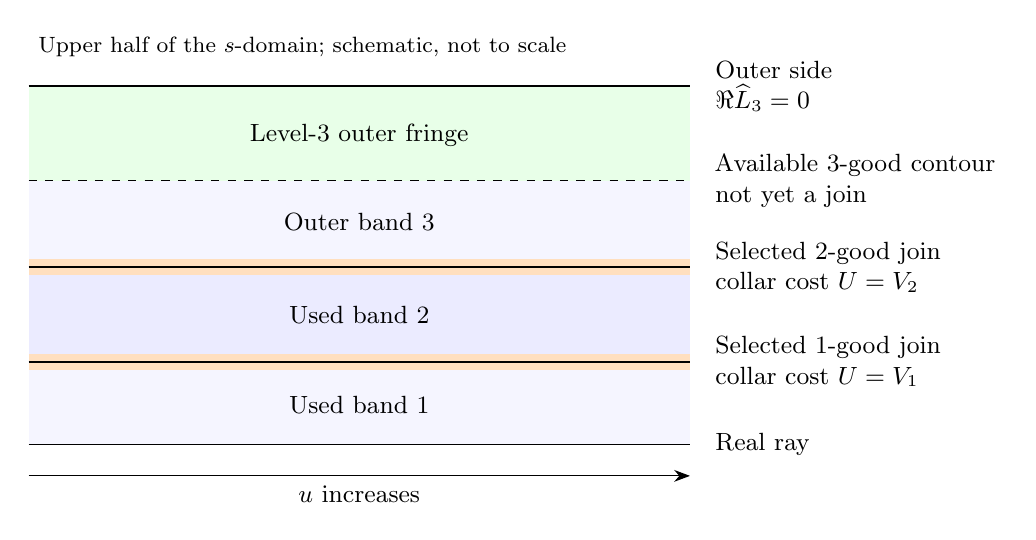
\begin{tikzpicture}[
  x=1cm,y=1cm,
  every node/.style={font=\small},
  boundary/.style={semithick},
  annotation/.style={anchor=west,align=left,text width=3.6cm},
  direction/.style={-{Stealth[length=2mm]},thin}]
\fill[blue!4] (0,0) rectangle (8.4,1.05);
\fill[blue!8] (0,1.05) rectangle (8.4,2.25);
\fill[blue!4] (0,2.25) rectangle (8.4,4.55);
\fill[green!9] (0,3.35) rectangle (8.4,4.55);
\fill[orange!25] (0,0.95) rectangle (8.4,1.15);
\fill[orange!25] (0,2.15) rectangle (8.4,2.35);

\draw[boundary] (0,0)--(8.4,0);
\draw[boundary] (0,1.05)--(8.4,1.05);
\draw[boundary] (0,2.25)--(8.4,2.25);
\draw[boundary,dashed] (0,3.35)--(8.4,3.35);
\draw[boundary] (0,4.55)--(8.4,4.55);

\node at (4.2,0.5) {Used band $1$};
\node at (4.2,1.65) {Used band $2$};
\node at (4.2,2.82) {Outer band $3$};
\node at (4.2,3.92) {Level-$3$ outer fringe};

\node[annotation] at (8.6,0) {Real ray};
\node[annotation] at (8.6,1.05)
  {Selected $1$-good join\\collar cost $U=V_1$};
\node[annotation] at (8.6,2.25)
  {Selected $2$-good join\\collar cost $U=V_2$};
\node[annotation] at (8.6,3.35)
  {Available $3$-good contour\\not yet a join};
\node[annotation] at (8.6,4.55)
  {Outer side\\$\Re\widehat L_3=0$};

\draw[direction] (0,-0.4)--(8.4,-0.4)
  node[midway,below] {$u$ increases};
\node[anchor=west,font=\footnotesize] at (0,5.05)
  {Upper half of the $s$-domain; schematic, not to scale};
\end{tikzpicture}
\caption{Coupling through level $p=3$; the analogous lower half is
omitted.  Each inner band $j<3$ ends at its selected level-$j$ good
join, whose smoothing cost is $U=V_j$.  Only the outer band $3$
continues through its outer fringe to the level-$3$ side.  The dashed
$3$-good contour is available for the next transition and is not yet
a join of this coupling.  Shaded collars mark the two join sources;
interior cutoff sources are not displayed.}
\label{fig:coupled-bands}
\end{figure}


\begin{lemma}[Holomorphic proxies and Cauchy correction]
\label{lem:separation-proxies}
On a coupled level-$p$ domain, the rates of indices $l\geq p$
have holomorphic proxies $\widehat Z_l=Z_l+o(1)$, uniformly on a
slightly smaller domain.  Their logarithms have the prescribed
lifted determinations.  Where needed, $f_{p-1}$ also has an
absolute $o(1)$ holomorphic proxy.  The level-$p$ side can be
defined by $\Re\widehat L_p=0$, with
\[
 \widehat L_p=\widehat Z_p-A\sum_{l>p}\widehat Z_l
                 -\frac{\widehat Z_p}{(\log\widehat Z_p)^K}.
\]
All the angular comparisons and real-part domination estimates
of Section~\ref{sec:flags} remain valid on the resulting component
containing the real ray.

If $a(s)$ is a $\bar\partial$ source in a domain contained in a
fixed-width strip and $|a(s)|\leq M e^{-u}$ for $u\geq u_b$,
its Cauchy transform has norm at most $C M e^{-u_b}$, with $C$
depending only on the strip width, and tends uniformly to zero
as $u\to\infty$ on that fixed domain.  The norm bound is also
uniform over families with a common $M$ and strip width; in
particular it tends to zero when their left starts $u_b$ tend
to infinity.  These statements apply as well after multiplication
by a holomorphic gauge whenever its source has the displayed
envelope.
\end{lemma}

\begin{proof}
Here and below sources are extended by zero when forming their
area Cauchy transforms; the identity for $\bar\partial$ holds in
the interior.  For an evaluation point $s$, split the integral
against $1/(\pi(s-\zeta))$ into $|s-\zeta|<1$ and its complement.
The first kernel has bounded integral on the unit disk and the
second has modulus at most one.  Thus
\[
 \left|\frac1\pi\iint
        \frac{a(\zeta)}{s-\zeta}\,\dd A(\zeta)\right|
 \leq C\|a\|_\infty+C\|a\|_1
 \leq C M e^{-u_b}.
\]
Subtracting the transform makes a $C^1$ function holomorphic.
The small norm and decay on a fixed domain are distinct assertions.
For the latter, fix $R>u_b$ and split $a=a_{\leq R}+a_{>R}$
according to the real coordinate of its argument.  For $u>R+1$,
the first transform is bounded by
\[
 \frac{\|a_{\leq R}\|_1}{\pi(u-R)},
\]
uniformly in $v$.  The preceding near-kernel and far-kernel
estimate bounds the second transform by $CM e^{-R}$.
First let $u\to\infty$ with $R$ fixed, then let $R\to\infty$.
This proves the asserted absolute $o(1)$ on a fixed path without
asserting any pointwise exponential decay rate for the correction.
For varying anchors we instead use the uniform norm estimate
with their far-starting domains; its constant is independent of
the anchor when the source envelope and strip width are common.

We verify that the rate sources have the required small envelope.
A cutoff with leading index $\sigma(r)<p$, active on an inner
band $j$, has
\begin{equation}\label{eq:separation-early-logcost}
 \Re f_{r,j}\geq
 c\frac{Z_{\sigma(r)}(u)}{\operatorname{polylog}Z_{\sigma(r)}(u)}.
\end{equation}
Indeed, if $\Lambda_{\sigma(r)}\ll\Lambda_j$, its leading
cosine is bounded below; otherwise
$\Lambda_j=O(\operatorname{polylog}Z_{\sigma(r)})$ and
\eqref{eq:separation-inner-cosine} gives the assertion.
Later terms in its affine log relation are negligible by the
real-part comparisons of Lemma~\ref{lem:flags-contours}.
For a secondary cosine, the loss is bounded unless its rate
derivative is comparable with $\Lambda_j$.  In that case its
negative logarithm is $O(\log(2+\Lambda_k))$ and is absorbed by
\eqref{eq:separation-early-logcost}.  In particular the log-cost
dominates $f_l$ for $l>\sigma(r)$; for $\sigma(r)=p-1$ it
still dominates $f_{p-1}$, since
$f_{p-1}=\log Z_{\sigma(r)}$.

For $\sigma(r)\geq p$, positivity and the polynomial angular
buffer in \eqref{eq:separation-barrier} give $U\gg f_p$;
the more quantitative verification is included in
Lemma~\ref{lem:separation-source-ratios}.  Join costs also satisfy
$V_j\gg f_p$ for $j<p$.  All these statements hold uniformly
on the coupled domain; they imply in addition $U/e^u\to\infty$.
Differentiating a later rate through its triangular formula
introduces only a fixed finite product of later rates, of
logarithmic size $O(f_p)$, as well as the allowed background
losses.  These factors can therefore be absorbed into $e^{-cU}$.
The $\bar\partial$ derivatives of all rates $l\geq p$ are bounded
by arbitrarily small multiples of $e^{-u}$ far enough out.
The preceding integral constructs their absolute $o(1)$ proxies.

The continuous lifted logarithm of $Z_p$ and the estimate
$\widehat Z_p/Z_p=1+o(1)/Z_p$ give a continuous logarithm of
$\widehat Z_p$; since $\widehat Z_p$ is holomorphic and nonzero,
this logarithm is holomorphic.  Its difference from $f_p$ is
exponentially small in $f_p(u)$.  If $f_{p-1}$ is free it is
already holomorphic.  Otherwise its exact affine expression in
later rates and a bounded background admits the same correction.

Construct these corrections first on the piecewise domain with
extra room.  Near vertical, the inward rotation in $Z_p/f_p^K$
has positive real part of size at least
$c|Z_p|/f_p(u)^{K+1}$.  This tends to infinity faster than every
fixed power of $f_p(u)$ and overwhelms the absolute corrections.
The plane comparisons of Lemma~\ref{lem:flags-contours} show that
$\Re\widehat L_p$ reaches zero within the available room after
increasing $A$ and decreasing $K$.  Its positive component has
the asserted sides and comparisons.  Neither this argument nor
the maximum principles below requires a globally one-to-one
map $s\mapsto\log\widehat Z_p$.
\end{proof}

\begin{lemma}[Propagation of coupled growth]
\label{lem:separation-growth}
Suppose the first $p-1$ transitions have been isolated and coupled.
Their coupled function has the level-$p$ bound
\begin{equation}\label{eq:separation-coupled-growth}
 \log^+|G|\leq C\Re Z_p+CD_{p-1},
\end{equation}
with the exceptional term absent on the outer side and on
simultaneous safe columns.  If a level-$p$ term is isolated on a
good collar with exponentially small error and coupled to its
child, the corresponding level-$(p+1)$ function has the analogous
bound, after a fixed backstep.  At a terminal transition it is
bounded.  All old joins and source types are preserved.
\end{lemma}

\begin{proof}
The assertion starts with the raw estimates.  Write $n=p+1$.
On the chosen $p$ collar the new coupled function equals its raw
outer child up to $O(e^{-cV_p})$.  Divide it holomorphically by
$\exp(C'\widehat Z_n)$, choosing $C'$ to absorb the child's
$\Re Z_n$ growth.  Old sources, including derivatives of fixed
normalizations, remain exponentially small.  Subtract their
Cauchy transform.  The lateral boundary logarithm is then at
most $CD_p+O(1)$, while the old interior bound gives logarithmic
growth $O(\Re Z_p)$ plus a path constant.

Choose a common safe left column $u_b$ in a fixed backstep.
There the old bound costs $O(e^{f_p(u_b)})$.  Put
$X+iY=\log\widehat Z_p$.  On the good-contour domain the positive
harmonic functions
\begin{equation}\label{eq:separation-growth-barriers}
 \delta\Re(\widehat Z_p e^{a_0s}),\qquad
 C_0e^{f_p(u_b)}e^{-\kappa(X-f_p(u_b))}\cos(\kappa Y)
\end{equation}
are respectively an infinity barrier and a left boundary barrier.
Take $0<\kappa<1$.  The small $a_0>0$ is chosen relative to the
good-contour constant: $a_0|v|$ is smaller than half the angular
margin $\epsilon_p/\Lambda_p$, so the first real part is positive.
It dominates the growth at infinity for every fixed $\delta>0$.
Apply the logarithmic maximum principle on bounded truncated
components, then let the right boundary tend to infinity and
$\delta$ decrease to zero.  The remaining left contribution tends
to zero if a fixed backstep was chosen with
$f_p(u)>Bf_p(u_b)$ for a sufficiently large fixed $B$; such
backsteps exist by Lemma~\ref{lem:flags-path}.  Restoring the
divisor and the small Cauchy correction proves
\eqref{eq:separation-coupled-growth} with $p$ replaced by $n$.

The raw outer part already has the safe-column improvement.
To carry it through the replaced inner wedge, if $D_p$ is not
absorbed by the new rate bound, use the safe collar on the box
$|X-f_p(u_*)|\leq R$, where $R=C_1\log(2+D_p)$.
The end boundary loss $CD_p$ is majorized by a constant times
\[
 D_p\frac{\cosh(\kappa(X-f_p(u_*)))\cos(\kappa Y)}
               {\cosh(\kappa R)}.
\]
Choose the fixed $C_1$ so that this is bounded at $X=f_p(u_*)$.
The lateral collar has the improved bound by hypothesis; sources
remain small.  The box lies in the available range because
$R=o(f_p)$.  The maximum principle therefore removes $D_p$ on
the column.  The outer side improvement is raw.  At $p=m$ omit
the divisor and use bounded ordinary terminal coefficients;
the same proof gives boundedness.  A finite number of steps uses
only finitely many safe columns and labels, as required.
\end{proof}

\subsection{The source comparisons}

The growth bound is now available for a fixed coupled domain.  To
improve a zero subtree, we will multiply its function by
$\exp(H\widehat L_n-C\widehat Z_n)$, with $H>0$ and fixed $C$.
Write $x=\Re\widehat L_n$.  A source of precision $e^{-cU}$ then
has size at most $\exp(Hx-cU)$ after the fixed losses are absorbed.
Thus the ratio $U/x$ controls how large a weight $H$ the sources
permit.

For a target with value $x_a>0$, separate sources with
$x\geq\rho x_a$ from those with $x<\rho x_a$, where $\rho>0$
is fixed and small.  A lower bound for $U/x$ on the first set
pays the weight there; the second set costs at most
$\rho Hx_a$.  The following lemma gives the required lower bounds
in the two possible slope regimes.  It also proves a common
integrable envelope for a spare factor $e^{-cU/2}$.  This second
estimate makes the constant in the Cauchy correction bound independent
of $H$.

\begin{lemma}[Source ratios]\label{lem:separation-source-ratios}
In a coupled level-$n$ domain put $x=\Re\widehat L_n$.
For $n>1$ write
\[
 i=n-1,\qquad g=f_i-f_n,\qquad
 r_0=\frac{g'(u_a)}{\Lambda_n(u_a)},\qquad g_0=g(u_a).
\]
At a target on a sufficiently vertical level-$i$ collar, and
through its further fringe,
\begin{equation}\label{eq:separation-target-x}
 x_a\asymp\Re Z_n(s_a)
       \asymp e^{f_n(u_a)}\frac{r_0}{1+r_0}.
\end{equation}
For every fixed $\rho>0$ and every fixed upper bound on $r_0$,
every coupled source satisfying $x\geq\rho x_a$ obeys
\begin{equation}\label{eq:separation-ratio-small}
 \frac{U}{x}\geq c\frac{e^{g_0}}{g'(u_a)}.
\end{equation}
When $r_0$ is bounded below by a positive constant this also holds
for central targets with $x_a\asymp e^{f_n(u_a)}$.

For large $r_0$ and central targets with
$x_a\asymp e^{f_n(u_a)}$, one has instead
\begin{equation}\label{eq:separation-ratio-large}
 \frac{U}{x}\geq e^{c g_0}
 \quad\hbox{on sources with }x\geq\rho x_a.
\end{equation}
For a fixed coupled calculation, $U/e^u\to\infty$ and
$U/x\to\infty$ uniformly on its sources at infinity.
These comparisons are unchanged by the absolute proxy errors.
\end{lemma}

\begin{proof}
All estimates can first be made with the piecewise rates; their
buffer tends to infinity, so the $o(1)$ corrections have no
effect.  Write $t=f_n(u)$ and $\lambda=\Lambda_n(u)$, with a
subscript $0$ for the target.  From
Lemma~\ref{lem:flags-path},
\begin{equation}\label{eq:separation-rate-derivatives}
 c t\leq\lambda\leq t\operatorname{polylog}t,
 \qquad
 \left|\frac{\dd\log\lambda}{\dd t}\right|
       \leq\frac{\operatorname{polylog}t}{t}.
\end{equation}
At the target the angle of $f_n$ differs from that of $f_i$ by
the gain $g'/\Lambda_i$.  Since $g'\to\infty$, the fixed
good-contour margin is negligible in comparison.  Later real
phases are negligible against $\Re Z_n$.  This proves
\eqref{eq:separation-target-x}; the same is true if the level-$i$
angle is moved farther toward vertical.  Background jet errors
are swallowed by that gain, by
Lemma~\ref{lem:flags-background}.  In particular this gain is
larger than the polynomial buffer needed for the level-$n$ side.

\emph{Bounded target slopes and join sources.}
Suppose first that $r_0\leq R$ with $R$ fixed.
The source constraint and $x\leq Ce^t$ give
\begin{equation}\label{eq:separation-backward-t}
 t\geq t_0-O(1)-\log(1+1/r_0).
\end{equation}
Since $g'_0\geq cg_0\to\infty$,
$r_0\geq c/\lambda_0$, so the possible backward interval has
length $O(\log\lambda_0)=O(\log t_0)$.  On that interval
$\lambda\asymp\lambda_0$ by
\eqref{eq:separation-rate-derivatives}.  The gap estimates also give
\[
 \left|\frac{\dd\log g'}{\dd t}\right|
   =\left|\frac{g''}{g'\lambda}\right|
   \leq\frac{\operatorname{polylog}t_0}{t_0},
\]
because $g\leq g_0\leq C_R\lambda_0$ in a backward interval.
Consequently $g'\asymp g'_0$, and its integrated loss satisfies
\begin{equation}\label{eq:separation-gap-backstep}
 g(u)\geq g_0-O_R(1),
\end{equation}
since $r_0\log(1+1/r_0)$ is bounded on $(0,R]$.
At forward points,
\[
 \frac{\dd}{\dd u}\log\frac{e^g}{g'}
       =g'-\frac{g''}{g'}>0
\]
eventually, using $g'\geq cg$ and the polynomial-logarithmic
bound on $g''/g'$.  Thus in both directions
$e^g/g'\geq c_R e^{g_0}/g'_0$ whenever the source constraint
can matter.

A join at $j<n$ has $U=V_j$.  With $J=f_j-f_n$, the collar
comparisons give
\[
 x\leq C e^{f_n}\frac{1+J'}{\Lambda_j},\qquad
 \frac{U}{x}\geq c\frac{e^J}{J'}.
\]
Write $J=g+\Delta$, $\Delta=f_j-f_i\geq0$.  If $j=i$,
$\Delta=0$; otherwise $\Delta'\leq\Delta\operatorname{polylog}\Delta$.
Since $g'\to\infty$, exponential growth in $\Delta$ absorbs
the possible $\Delta'$ loss, giving
\[
 \frac{e^J}{J'}\geq c\frac{e^g}{g'}.
\]
This proves \eqref{eq:separation-ratio-small} for joins.

\emph{Cutoff sources at bounded target slopes.}
Consider a cutoff source, with earlier label $r<j\leq n$,
$F=f_r(u)$ and $\sigma=\sigma(r)$.  If $\sigma<n$, estimate
\eqref{eq:separation-early-logcost} applies on its own inner
band.  Because $\sigma\leq i$ and
$f_i\leq\log Z_\sigma$, its log-cost exceeds $f_i$ by an
unbounded factor.  The secondary cosine loss described there
does not change this conclusion.  It is therefore stronger
than both required ratios.

Suppose $\sigma\geq n$.  There are four estimates to check.
If $F\leq t^{3/2}$, the angular scale is at most
$C/\lambda$, and Taylor's formula together with the fixed
derivative bounds gives
\[
 \Re f_{r,j}=F+O\!\left(
              \frac{F\operatorname{polylog}F}{\lambda^2}
                         \right)=F+o(1).
\]
For a simple cost, or a mixed cost with $k\geq n$, division
by $x$ therefore gives
\begin{equation}\label{eq:separation-small-F}
 \frac{U}{x}\geq c e^{F-f_n}.
\end{equation}
For $k<n$, the source lies on an inner band $j\leq k$ ending
at its good join.  Its secondary cosine is at least
$c/\Lambda_k$, and the angular comparison yields
\begin{equation}\label{eq:separation-cosine-ratio}
 \frac{\cos(\Im f_{k,j})}{\cos(\Im f_{n,j})}
       \geq\frac{c}{1+\Lambda_k-\Lambda_n}.
\end{equation}
Since $r<j\leq k\leq i$, we have $F\geq f_k$.
Set $\Delta=f_k-f_i\geq0$.  The resulting ratio is at least
\[
 c\frac{e^{g+\Delta}}{1+g'+\Delta'}
       \geq c\frac{e^g}{g'}.
\]
Together with the backward and forward comparisons already
proved, this settles the small-$F$ case.

If $t^{3/2}<F\leq t^3$, the leading affine relation gives
$F\asymp Z_\sigma$ and
$f_\sigma=\log F+O(1)=O(\log t)$.  Hence
$\Lambda_\sigma/\lambda\to0$, the angle of its leading rate
is small, and
\begin{equation}\label{eq:separation-middle-F}
 \Re f_{r,j}\geq cF.
\end{equation}
If $F>t^3$ and $\sigma>n$, the leading cosine is at least
$c/\lambda$; later affine terms are negligible.  Thus
\begin{equation}\label{eq:separation-large-F}
 \Re f_{r,j}\geq cF/\lambda.
\end{equation}
Finally, if $\sigma=n$, the large $A$ in the side equation
absorbs the later affine terms and leaves the buffer:
\begin{equation}\label{eq:separation-sigma-n}
 \Re f_{r,j}\geq cx+
                    c\frac{e^t}{t^{K+1}}.
\end{equation}
This also holds on the relevant inner contours.

For bounded target slopes,
$g_0\leq C_R\lambda_0$.  At backward sources the possible
drop in $t$ is only $O(\log t_0)$; at forward sources
$g_0\leq C_R\lambda_0\leq t\operatorname{polylog}t$.
Each of \eqref{eq:separation-middle-F}--\eqref{eq:separation-sigma-n}
therefore dominates $t+g_0+\log(2+F)$.  In
\eqref{eq:separation-large-F} use
$F/\lambda\geq t^2/\operatorname{polylog}t$ and
$\log F\leq t+O(1)$ when $\sigma>n$.
The negative logarithm of a secondary cosine is either bounded
or $O(\log(2+F))$: if $k<n$, use its inner-band lower bound;
if $k\geq n$, use the side's polynomial buffer and ordered
angles.  All those losses and division by $x\leq Ce^t$ are
absorbed.  This proves \eqref{eq:separation-ratio-small} for
all cutoff costs, uniformly even when $r_0\to0$.

\emph{Large target slopes.}
Now take a large target slope and a central target.  The source
constraint implies $t\geq t_0-O(1)$.  The adjacent-gap bound
$g'/g\leq C\lambda$ implies
\begin{equation}\label{eq:separation-large-backstep}
 g(u)\geq c g_0
 \quad\hbox{whenever }t\geq t_0-O(1).
\end{equation}
The join calculation and the small-$F$ calculation above give
$U/x\geq e^{c g_0}$: their derivative denominators are only
polynomial-logarithmic in the corresponding diverging gaps.
For $\sigma=n$, the target relation gives
$g_0\leq f_i(u_a)\leq f_r(u_a)\leq Ce^{t_0}$.
Thus \eqref{eq:separation-sigma-n} and the source constraint
$x\geq\rho x_a\asymp e^{t_0}$ leave a fixed positive multiple
of $g_0$ in the log-cost.  The buffer term absorbs $t$ and the
secondary cosine losses, giving the same ratio.

It remains to justify the extra angular loss when $F>t^{3/2}$
and $\sigma>n$.  Put
\[
 J=f_n-f_\sigma,\quad
 d=\frac{J'}{\lambda}=1-\frac{\Lambda_\sigma}{\lambda},\quad
 \eta=\cos(\Im f_{n,j}),\quad q=\min(1,\eta+d).
\]
The leading real contribution satisfies
\begin{equation}\label{eq:separation-angular-F}
 \Re f_{r,j}\geq cF(\eta+d).
\end{equation}
Moreover $d\geq c/\lambda$, and so
$L=\log(1/q)=O(\log t)$.  The gap derivative bounds give
\begin{equation}\label{eq:separation-logd}
 \left|\frac{\dd\log d}{\dd t}\right|
 =\left|\frac{J''}{J'\lambda}
                    -\frac{f_n''}{\lambda^2}\right|
       \leq\frac{\operatorname{polylog}t}{t}.
\end{equation}
Decrease $t$ to $t-L$ and denote the corresponding real position
by $u'$.  The quantity $d$ changes by a bounded factor (in fact
by $1+o(1)$).  Since $q\geq d$,
$dL\leq d\log(1/d)$ is bounded.  Integrating
$\dd f_\sigma/\dd t=1-d$ now gives
\begin{equation}\label{eq:separation-angular-backshift}
 Z_\sigma(u')
  =Z_\sigma(u)
     \exp\!\left(-L+\int_{t-L}^{t}d(\tau)\,\dd\tau\right)
  \asymp qZ_\sigma(u).
\end{equation}
Because $x\leq Ce^t\eta\leq Ce^tq$ and
$x\geq\rho x_a$, one has $t-L\geq t_0-O(1)$.
The indices $r<j\leq n=i+1$ imply $r\leq i$; hence
\[
 g(u')\leq f_i(u')\leq f_r(u')\asymp Z_\sigma(u').
\]
Combining this with \eqref{eq:separation-large-backstep} and
\eqref{eq:separation-angular-backshift} proves
$F(\eta+d)\geq c g_0$.
Independently, \eqref{eq:separation-middle-F} or
\eqref{eq:separation-large-F} gives
$\Re f_{r,j}\gg t+\log(2+F)$.
These two lower bounds, each used with a sufficiently small
fixed fraction of the log-cost, absorb division by $x$ and all
secondary cosine losses, leaving $\log(U/x)\geq c g_0$.
This proves \eqref{eq:separation-ratio-large}.

\emph{The common integrable envelope.}
The same estimates without a target show the asserted uniform
growth at infinity.  For joins,
$U/x\geq ce^{f_j-f_n}/(f_j-f_n)'\to\infty$.
For cutoffs with small $F$, the bound is of this form with a
larger gap; the other cases have a log-cost dominating $f_n$
or its relevant angularly diminished value.  All costs dominate
$e^u$ uniformly over the controlled finite-request families in
Definition~\ref{def:packet}.  More explicitly, on a join
\[
 \log U=f_j-\log\Lambda_j\geq\tfrac12 f_j
                         \geq\tfrac12 e^u
\]
eventually.  For a cutoff, the small-$F$ estimate leaves
$F-O(\log(2+F))\geq c f_n$ after the secondary cosine loss;
the intermediate and large-$F$ estimates and the buffer in
\eqref{eq:separation-sigma-n} leave at least $c f_n$ as well.
The early-index estimate is stronger.  Thus, after decreasing
a fixed $c>0$ for the finite source list,
\begin{equation}\label{eq:separation-uniform-source-envelope}
 U\geq\exp(c e^u).
\end{equation}
Every threshold here depends only on the finite quantitative
controls specified in the definition.  In particular, for any
fixed source precision constant $c_*>0$, the residual factor
$e^{-c_*U}$ has a common envelope $M e^{-u}$ on the full
forward domains, with $M$ independent of their anchors.
The stipulated uniform $o(U)$ absorption permits the same
conclusion after all fixed losses.  These constants are also
independent of any subsequently chosen weight parameter.
\end{proof}

\subsection{The zero-subtree estimate}

\begin{lemma}[Weighted maximum estimate]\label{lem:separation-weighted}
Let $G$ be coupled through level $n$ with the growth bound of
Lemma~\ref{lem:separation-growth}.  Suppose that on the real ray
\begin{equation}\label{eq:separation-preliminary}
 |G(u)|\leq C_N e^{-NZ_n(u)}
 \quad(u\geq u_N),\qquad\hbox{for every fixed }N>0.
\end{equation}
The constants $C_N,u_N$ can depend arbitrarily on $N$.
Fix the coupled functions, its joins, a safe left column, and
the full domain $x=\Re\widehat L_n>0$.  There are fixed
$C,C_0,c>0$ such that for every $H>0$ and every point of that
domain,
\begin{equation}\label{eq:separation-weighted}
 \log|G|+Hx-C\Re\widehat Z_n
 \leq C_0+\max\left\{
 H\sup_{\rm left}x,
 \sup_{\rm sources}(Hx-cU/2),\ 0\right\}.
\end{equation}
In particular $C_0$ is independent of $H$, $C_N$, and $u_N$.
When $n=1$ there are no sources, and
\eqref{eq:separation-preliminary} implies exact vanishing.
\end{lemma}

\begin{proof}
\emph{Correcting the weighted sources.}
Choose $C$ greater than the fixed coefficient in the coupled
growth estimate on safe columns and the side.  Multiply $G$ by
the holomorphic gauge
\[
 \exp(H\widehat L_n-C\widehat Z_n).
\]
Its side modulus is bounded independently of $H$ because $x=0$;
its left boundary logarithm is at most
$H\sup_{\rm left}x+O(1)$.  With constants decreased to absorb
the fixed losses, its sources have modulus at most a finite sum
of $\exp(Hx-cU)$.  Set
\[
 K_H=\max\{0,\sup_{\rm sources}(Hx-cU/2)\}.
\]
The source-ratio lemma makes $K_H$ finite for every fixed $H$.
Crucially, keep half the negative cost:
\begin{equation}\label{eq:separation-spare-cost}
 e^{Hx-cU}\leq e^{K_H}e^{-cU/2}.
\end{equation}
The last factor is bounded by a fixed multiple of $e^{-u}$ and
is integrable on the bounded-width domain, because
$U/e^u\to\infty$.  Lemma~\ref{lem:separation-proxies} thus
gives a Cauchy correction of norm at most $C_1e^{K_H}$,
where $C_1$ is independent of $H$.  Let $F_H$ be the resulting
holomorphic function.
By \eqref{eq:separation-uniform-source-envelope}, $C_1$ is
uniform for the controlled finite-request families as well;
the bound uses their full forward domains, not just a window
about the target.  Their possibly different return times to
smaller ordinary neighborhoods do not enter this constant.

\emph{Boundedness for each fixed weight.}
For each fixed $H$, preliminary real decay makes the weighted
function bounded on the real ray: choose $N$ larger than the
fixed multiple of $H+C$ needed there, and include the finite
interval before $u_N$ in its bound.  This bound can depend on
$H$ in an uncontrolled way; we do not use it in the final
estimate.  To see that $F_H$ is bounded on each half-domain,
write $X+iY=\log\widehat Z_n$.  Its logarithmic growth is
$O_H(e^X)$ plus a path constant.  On the upper half use the
positive harmonic barrier
\[
 \delta e^{aX}\cos(a(Y-\pi/4)),\qquad 1<a<2,
\]
and on the lower half use
$\delta e^{aX}\cos(a(Y+\pi/4))$.
The side angles tend to $\pm\pi/2$, so a sufficiently far
start makes both barriers positive on their respective
half-domains.  They dominate the infinity growth.  The maximum
principle on finite truncations and then $\delta\downarrow0$
proves boundedness on each half, hence on the full domain.

\emph{Removing the preliminary constants.}
Now apply the bounded maximum principle to that \emph{full}
domain.  The real ray is no longer a boundary.  One can justify
the infinite-domain principle by
$\delta e^{a'X}\cos(a'Y)$, $0<a'<1$, before letting
$\delta\downarrow0$.  Only the side and the fixed safe left
column remain.  After restoring the Cauchy correction their
bounds give \eqref{eq:separation-weighted}, with an additive
constant depending on $C_1$ and the fixed data alone.  This
explains why the arbitrary constants in
\eqref{eq:separation-preliminary} disappear.

For $n=1$, choose a fixed backstep so that the target's positive
$x_a$ is larger than $\sup_{\rm left}x$.
There is no source term, and
\eqref{eq:separation-weighted} gives
\[
 \log|G(s_a)|\leq C_0+C\Re\widehat Z_1(s_a)
              -H(x_a-\sup_{\rm left}x).
\]
Letting $H\to\infty$ proves $G(s_a)=0$.  Every sufficiently
far real target permits this construction, giving the asserted
identity on the real locus.
\end{proof}

\begin{lemma}[Upgrade at the preceding transition]
\label{lem:separation-upgrade}
For $n>1$, under the hypotheses of
Lemma~\ref{lem:separation-weighted}, the outer packet of $G$
satisfies $|G|\leq Ce^{-cV_{n-1}}$ on sufficiently vertical
level-$(n-1)$ collars and their further fringe.
\end{lemma}

\begin{proof}
Put $i=n-1$ and use the notation of the source-ratio lemma.
A fixed backstep can make
\begin{equation}\label{eq:separation-left-small}
 \sup_{\rm left}x\leq\rho x_a
\end{equation}
for any chosen small fixed $\rho>0$.
Indeed, $f_n$ on that column can be made a fixed factor smaller
than $f_n(u_a)$, whereas
$x_a\geq c e^{f_n(u_a)}/\Lambda_n(u_a)$ at the target.
Safe columns exist in the needed fixed intervals.

\emph{Bounded slopes.}
If $r_0$ is bounded, choose
\[
 H=c_1\frac{e^{g_0}}{g'_0}
\]
with $c_1>0$ sufficiently small.  On sources with
$x\geq\rho x_a$, \eqref{eq:separation-ratio-small} gives
$Hx-cU/2\leq0$; on the remaining sources it is at most
$\rho Hx_a$.  Thus the maximum on the right of
\eqref{eq:separation-weighted} is at most $\rho Hx_a$.
At the target $\Re\widehat Z_n\asymp x_a$ and $H\to\infty$,
so the subtracted fixed growth term is negligible.  Finally,
\begin{equation}\label{eq:separation-bounded-slope-scale}
 Hx_a\asymp
 \frac{e^{g_0}}{g'_0}e^{f_n(u_a)}
        \frac{g'_0/\Lambda_n(u_a)}{1+g'_0/\Lambda_n(u_a)}
 =\frac{e^{f_i(u_a)}}{\Lambda_i(u_a)}=V_i(u_a).
\end{equation}
This proves the result for bounded slopes, uniformly down to
$r_0=0$ as a limiting regime.  When $r_0$ stays in a fixed
compact subinterval of $(0,\infty)$ the same proof applies
to central level-$n$ targets.

\emph{Large slopes: decay in the central region.}
For large slopes, first use central level-$n$ targets.
Take $H=\exp(c_2g_0)$ with $c_2$ smaller than the constant
in \eqref{eq:separation-ratio-large}.  Exactly the preceding
argument gives
\begin{equation}\label{eq:separation-central-large}
 |G(s_a)|\leq
       \exp\{-\exp(c_3 f_i(u_a))\}
\end{equation}
for some fixed $c_3>0$, since
$Hx_a\geq c\exp(f_n(u_a)+c_2g_0)$ and
$f_i=f_n+g_0$.  This estimate is weaker than the desired one
at the preceding transition, so a second maximum principle is
needed.

\emph{Large slopes: transfer to the preceding fringe.}
Use the holomorphic coordinate function
$X+iY=\widehat f_i$.  Work first in the local tube
$|v|<2W/\Lambda_i(u)$, with fixed slack at its real end columns,
and take the component meeting the real ray of the inverse
image, within this tube, of the rectangle
\[
 X_0-1<X<B_1X_0,\qquad |Y|<W,
 \qquad X_0=f_i(u_a),
\]
where $W$ is a large fixed number.  Stop at a right real column
if $\Lambda_i/\Lambda_n$ first falls to a fixed
$M_0\gg W$.  For a sufficiently large starting ratio, its
short left extension retains a large ratio by the derivative
bounds.  On the tube's two angular walls the path estimates and
the absolute proxy correction give
$Y=\pm2W+o(1)$ and $X=f_i(u)+o(1)$.
The selected component, where $|Y|<W$, cannot meet those walls.
There are therefore no additional angular boundary pieces to
estimate.  All its points remain in this local tube and are
central for level $n$: their $f_n$ angle is at most
$O(W/M_0)$.
The level-$i$ target, with $|Y|\sim\pi/2$, is inside it.

Every source encountered in this rectangle has
\begin{equation}\label{eq:separation-rectangle-cost}
 U\geq c\frac{e^X}{\Lambda_i}.
\end{equation}
For joins this is the gap calculation above.  A cutoff with
$\sigma<n$ has the stronger bound
\eqref{eq:separation-early-logcost}.  If $\sigma\geq n$,
its leading angle is small.  With $F=f_r$ and $T=f_i$, the
case $F\leq T^{3/2}$ gives $\Re f_{r,j}=F+o(1)$ by the
Taylor calculation on the scale $W/\Lambda_i$.  Since
$r\leq i$, this pays $e^X$; a secondary cosine with $k\leq i$
costs at worst $\Lambda_k$, and
$\Lambda_k/\Lambda_i$ is absorbed by $e^{F-f_i}$ using
the same gap calculation as
\eqref{eq:separation-cosine-ratio}.  If $F>T^{3/2}$, use
that every phase of index at least $n$ has size
$O(W/M_0)$ throughout this rectangle.  The leading cosine
is bounded below, later affine terms remain negligible,
and $\Re f_{r,j}\geq cF$.  This exceeds
$T+\log(2+F)$ by an unbounded factor, paying every such
secondary loss.  This proves
\eqref{eq:separation-rectangle-cost}.

Take $\kappa=\pi/(2W)<c_3$, and let $w$ be the positive
harmonic function
\begin{equation}\label{eq:separation-strip-weight}
 w(X,Y)=c_4\frac{e^{X_0}}{\Lambda_i(u_a)}
      \sinh(\kappa(X-X_0+1))\cos(\kappa Y).
\end{equation}
It is the real part of a holomorphic function of
$\widehat f_i$ and vanishes on the left and horizontal sides.
The rate derivative bound implies
\begin{equation}\label{eq:separation-lambda-strip}
 \left|\frac{\dd\log\Lambda_i}{\dd X}\right|
      \leq\frac{\operatorname{polylog}X}{X}=o(1).
\end{equation}
Consequently, throughout the rectangle,
\[
 \frac{w(X,Y)}{e^X/\Lambda_i(X)}
 \leq Cc_4
       \exp(-(1-\kappa-o(1))(X-X_0))
\]
apart from the harmless one-unit left extension.  Choosing $c_4$
small makes the weight at most a fixed small fraction of every
source cost in \eqref{eq:separation-rectangle-cost}.

On a full right edge $X=B_1X_0$, the logarithm of the size of
$w$ is at most
$[1+\kappa(B_1-1)]X_0+O(\log\Lambda_i(u_a))$.
Choose
\begin{equation}\label{eq:separation-right-factor}
 B_1>\frac{1-\kappa}{c_3-\kappa}.
\end{equation}
Then \eqref{eq:separation-central-large} pays the whole
weight there.  If the domain was stopped at the bounded-ratio
column, the bounded-slope result
\eqref{eq:separation-bounded-slope-scale} pays it instead,
after reducing $c_4$ using
\eqref{eq:separation-lambda-strip}.  The other edges have
zero weight, and \eqref{eq:separation-central-large} bounds
$G$ there.

Multiply $G$ by the holomorphic gauge with real logarithm $w$.
Its sources retain an integrable negative half-cost, so their
Cauchy correction is bounded independently of the target.
The maximum principle on the bounded component therefore
bounds the weighted function by a fixed constant.  At the
target, the cosine in \eqref{eq:separation-strip-weight} is
bounded below and $\sinh\kappa>0$, so
$w(s_a)\geq cV_i(u_a)$.  This proves the desired
$e^{-cV_i}$ bound.  The argument uses only positive harmonic
functions pulled back by $\widehat f_i$ and works without
global coordinate injectivity.  It applies unchanged to the
farther level-$i$ fringe.  Nominal pointwise cutoff variants
differ there by errors with the same lower cost, so satisfy
the same bound.
\end{proof}

\subsection{Finite isolation and terminal comparison}



\begin{lemma}[One finite transition]\label{lem:separation-isolate}
Suppose a prefix is coupled through level $p$.  Fix a child
exponent $a$, and assume that every earlier child has an entire
zero subtree and satisfies the upgrade of
Lemma~\ref{lem:separation-upgrade} at level $p$.
Then a sufficiently vertical fixed good collar can be chosen so
that
\begin{equation}\label{eq:separation-isolate}
 e^{aZ_{p,p}}S^p_{\lambda_{<p}}
     =S^{p+1}_{\lambda_{<p},a}+O(e^{-cV_p})
\end{equation}
on both sides, with zero insertion if necessary.  It can be
coupled to that child while preserving all preceding joins.
\end{lemma}

\begin{proof}
Only finitely many children precede $a$ by left-finiteness.
For an earlier exponent $b<a$, its outer packet is
$O(e^{-c_bV_p})$ beyond its previously selected join.
On a more vertical good collar,
$\Re Z_p\asymp\epsilon_pV_p$.  Choose $\epsilon_p>0$
small enough that every finite multiplier
$\exp((a-b)\Re Z_p)$ is absorbed by half of the corresponding
$c_bV_p$.  This is a finite restriction.  The collar may also
be chosen beyond every earlier child's selected join and within
the allowed inward extension of the chosen child.

Take a transition budget larger than $a$ and use
\eqref{eq:separation-transition}.  For every included later
exponent $b>a$, its positive gap $b-a$ suppresses its raw
packet: on the $p$ collar
\[
 \Re Z_{p+1}=o(V_p),\qquad D_p=o(V_p),
\]
and there are only finitely many such terms.  The first estimate
is the contour hierarchy.  For the second, any uncapped
coefficient contributes at most $O(\log\Lambda_p)$ on a fixed
backstep, and $\log\Lambda_p=o(V_p)$; the same conclusion
holds along the ray.  The tail error is also
$O(e^{-cV_p})$ after increasing the budget if necessary.
These observations give \eqref{eq:separation-isolate}.

In the inner bands multiply the existing coupled function by
$\exp(a Z_{p,j})$, then switch on this collar to the selected
outer child.  On an old $j$ join, $j<p$, the new rate has real
part $o(V_j)$, so old seam errors persist.  Background changes
alter this fixed multiplier by a relatively exponentially small
amount there.  The source hypotheses handle all derivatives of
the interpolation and normalization.  The growth bound for the
new coupling follows from Lemma~\ref{lem:separation-growth}.
No new transition at an earlier inner band has been requested.
\end{proof}

\begin{lemma}[Comparison of terminal coefficients]
\label{lem:separation-terminal}
Suppose a complete exponent vector has been isolated on the two
sides and coupled, with all earlier subtrees passed as in
Lemma~\ref{lem:separation-isolate}.  Its two terminal ordinary
coefficients are the same analytic germ.  The fully normalized
coupled function tends to this germ on the real ray and through
the corresponding inner wedge and used bands.
\end{lemma}

\begin{proof}
By terminal growth propagation the normalized function is
bounded on the whole inner domain after a fixed backstep.
For a target family with real anchors $u_a\to\infty$, choose
safe left columns $u_b$ in fixed backstep intervals.  The finite
raw, background, and source data used by this terminal coupling
have common bounds on their full forward domains, by the
finite-request hypothesis.  In particular
\eqref{eq:separation-uniform-source-envelope} supplies a common
$M e^{-u}$ envelope for their corrected sources.  Their Cauchy
corrections therefore have norm at most $CM e^{-u_b}\to0$,
uniformly over the target family.  On a single fixed path the
compact-left and tail argument in
Lemma~\ref{lem:separation-proxies} gives the corresponding
vanishing at infinity.  Denote the corrected functions by $\widetilde G$; they are
holomorphic and uniformly bounded.
On the two outer collars their values approach, respectively,
$c_+(t)$ and $c_-(t)$, by the terminal transition.

We give the argument that these two boundary limits cannot
differ.  Fix an ordinary value $t_*$ in a sufficiently small
real neighborhood and take a family of tests approaching it
on every fixed $u$ window about the varying anchor.  Such tests
can return to $t_c$ at infinity: for example, on the needed
right half-strip use
\[
 t(s)=t_c+(t_*-t_c)e^{-\delta_a(s-u_a)},
 \qquad\delta_a\downarrow0,
\]
with the fixed backward range and ordinary neighborhood chosen
with slack.  Its fixed positive derivatives tend to zero and
it returns to $t_c$ on every chosen path.  Taking
$0<\delta_a\leq\delta_0$ gives common finite-jet bounds on
the entire forward domains, and $\delta_a\to0$ gives a
common small-jet modulus and convergence to $t_*$ on each
fixed target window.  The time of return to a smaller box may
diverge; that time is used only in the preliminary real
estimates, whose constants have already been removed by
Lemma~\ref{lem:separation-weighted}.

Write $X+iY=\log\widehat Z_m$.  For a fixed small $\eta>0$,
the boundary values on a window about the target are within
$\eta$ of the corresponding constants, once the anchor is
sufficiently far.  The $X$ distances from the target to both
ends of a fixed $u$ window tend to infinity by
Lemma~\ref{lem:flags-path}.  On that window apply the logarithmic
maximum principle to the difference from $c_+(t_*)$.
Its upper boundary is bounded by $\log\eta$, its lower
boundary by a fixed constant $\log M$, and its two ends by
the bounded growth estimate.  An affine function of $Y$
interpolates the lateral logarithmic bounds.  The actual angles
tend to $\pm\pi/2$; adding arbitrarily small relative angular
slack and decaying cosine barriers at the two ends yields, at
the real target,
\[
 \limsup\log|\widetilde G-c_+(t_*)|
       \leq\tfrac12\log\eta+\tfrac12\log M.
\]
For completeness, the end barriers may be taken as fixed
multiples of
$e^{-\kappa(X-X_-)}\cos(\kappa Y)$ and
$e^{-\kappa(X_+-X)}\cos(\kappa Y)$ with $0<\kappa<1$.
Their values at the target tend to zero.  First let the target
go to infinity, then let the angular slack and $\eta$ go to
zero.  The real-ray limit is $c_+(t_*)$.  Applying the same
argument from the lower boundary gives the limit $c_-(t_*)$.
Thus these two values coincide for every such real $t_*$.
The identity theorem for analytic germs makes the coefficients
equal.

With their common value on both lateral boundaries, apply the
same maximum principle to their difference from $\widetilde G$.
The lateral bound is now $\eta$ on both sides, so the estimate
holds uniformly across the entire inner wedge, including
targets approaching either boundary.  Restoring the vanishing
Cauchy correction changes nothing.  Uniformity on smaller
ordinary neighborhoods follows either from these estimates
with common finite slack or by applying the construction to
a putative sequence of violating ordinary inputs.  The same
argument uses the corresponding coupled determinations in the
already used bands, and proves their asserted convergence.
\end{proof}

\begin{proof}[Proof of Theorem~\ref{thm:separation}]
We describe the induction explicitly to keep its finite and
infinite requests separate.  A coupled prefix includes fixed
functions on the earlier inner bands, fixed selected joins,
the growth bounds, and the finite list of their source types.
An assertion about that prefix may request more accuracy
\emph{at infinity on its existing path}; it may not change
those already fixed functions or joins.

Induct downward on the level $n$.  The assertion to prove is:
for every coupled prefix whose entire level-$n$ subtree has
zero terminal data, the preliminary estimates
\eqref{eq:separation-preliminary} hold for all fixed $N$;
they imply the preceding-transition upgrade when $n>1$ and
exact vanishing when $n=1$.

At $n=m$, all ordinary child coefficients are zero.  For each
fixed budget the transition formula therefore gives arbitrary
exponential decay on a sufficiently vertical $m$ collar.
Equivalently insert a zero terminal child at any exponent
$a>N$, choosing the remainder budget greater than $a$.
The proof of growth propagation, applied after multiplication
by $e^{aZ_m}$, gives a bounded function in the inner wedge
after a fixed backstep.  On the real ray this is
$O(e^{-aZ_m})$, and hence implies
\eqref{eq:separation-preliminary} for the requested $N$.
No uniformity over $N$ has been used.  The weighted lemma and
the upgrade lemma now establish the induction assertion at
level $m$.

Suppose it is known strictly below level $n$ and consider an
entirely zero subtree coupled through level $n$.
Fix one finite requested real order $N$.  Choose an exponent
$a>N$ at this coordinate and insert a zero child there if
necessary, enlarging the transition budget beyond it.  There
are finitely many children earlier than $a$.  Pass them in
increasing order.  To pass one child, first isolate it on its
own sufficiently vertical good contour using
Lemma~\ref{lem:separation-isolate} and the upgrades already
obtained for its earlier siblings.  Its coupled subtree at
level $n+1$ is zero, so the induction hypothesis below $n$
gives its preliminary real estimates and its
$e^{-cV_n}$ upgrade.  This permits the next sibling to be
isolated.  Only finitely many siblings are needed before
reaching the inserted zero child $a$.

After isolating that child, the growth propagation lemma gives
on the real ray
\[
 |G(u)|\leq C\exp(-aZ_n(u)+CZ_{n+1}(u)+CD_n)
\]
when $n<m$, and the corresponding bound without the last
rate at $n=m$.  Since $Z_{n+1}=o(Z_n)$ and $D_n$ is a
constant on this path, this is the requested
$O(e^{-NZ_n})$ estimate sufficiently far out.  Alternatively
one may continue the zero child down to a terminal zero;
both constructions use only finitely many transitions for
this request.  We have proved all fixed preliminary orders
at level $n$, and can now apply
Lemma~\ref{lem:separation-weighted} and
Lemma~\ref{lem:separation-upgrade}.

There is no circular use of a stronger estimate at the current
level.  Preliminary orders at level $n$ invoke upgrades only
at level $n+1$; the height decreases each time.  Finite breadth
can grow with $N$, but the height is at most $m$.
Moreover all joins strictly preceding the child under
consideration remain fixed.  Higher requests need new labels
only at that child or deeper, and any new fixed later
multiplier costs $o(V_j)$ on an old $j$ join.  Thus the full
domain in the weighted lemma has fixed source estimates
independent of its multiplier $H$.  The preliminary real
estimates may start arbitrarily farther out as $H$ varies;
their constants disappear in
\eqref{eq:separation-weighted}.  This completes the downward
induction and, at $n=1$, proves the exact-zero assertion.

If the paired array is nonzero, choose its first nonzero
exponent $\lambda$.  At the first coordinate pass only the
finitely many earlier subtrees, all of which are zero by
definition of $\lambda$.  The established upgrades and
Lemma~\ref{lem:separation-isolate} isolate $\lambda_1$.
Repeat at its selected child, then at the next one.  This
finite process reaches the paired ordinary coefficients at
$\lambda$.  Lemma~\ref{lem:separation-terminal} proves their
equality and the real leading limit
\eqref{eq:separation-leading}.  It also proves the corresponding
limits for the coupled normalized determinations inside their
selected contours and along the bands already used.

It remains to justify the owning-fringe extension in the
statement.  Beyond a selected leading join the outer packet
is the one whose convergence was just proved.  In the finite
transition \eqref{eq:separation-transition}, every earlier
term still has its $e^{-cV_j}$ suppression on that more
vertical portion, and every later term has a strictly positive
current exponent.  Choose the fringe constant sufficiently
small for the finitely many earlier multipliers and choose
$A$ large enough that $\Re Z_j$ dominates the finite later
real-phase losses.  The transition remainder can be requested
to any fixed needed depth.  Thus the same normalized leading
estimate holds throughout that fringe.

In this last comparison rates in the two backgrounds must
also be compared.  Estimate
\eqref{eq:separation-background-fringe} is sufficient: triangular
differentiation of a fixed later rate $Z_k$, $k>j$, has
logarithmic sensitivity at most $C f_{j+1}$ in these variables,
whereas $\Re Z_j$ dominates every fixed power of $f_j$ on the
buffered side.  Hence the absolute change in each such later
rate is $o(1)$ after any fixed needed normalization.  The
extracted current factor is always kept at its own inner
background; it is not reevaluated at the next background.
On selected good joins the stronger $e^{-cV_j}$ comparison
already gave the same conclusion.  This proves the stated
fringe extension and finishes the theorem.
\end{proof}

\subsection{Uniformity for the differentiated calculus}

The preceding proof also supplies the uniform estimates needed when
ordinary tests vary with their anchors.  We collect their precise scope
here for the differentiated calculus in Section~\ref{sec:calculus}.

\begin{lemma}[Uniformity for a controlled finite request]
\label{lem:separation-family-uniformity}
Fix finitely many packet labels, transition budgets, coupled
joins, and normalizations, and a family of tests with the common
quantitative controls in Definition~\ref{def:packet}.  The fixed
labels used on the coupled domain must stay in their common
ordinary ranges throughout that domain.  Deeper labels used
only for preliminary real estimates may have smaller ranges
entered at a time depending on the member of the family.

The proxy, growth, source-ratio, and preceding-transition
estimates above have constants uniform in this family.  If
each member has the preliminary estimates
\eqref{eq:separation-preliminary}, no uniformity of their
$C_N,u_N$ or of their return times is needed for the weighted
estimate or its upgrades.  Terminal comparison is uniform at
receding anchors when the tests have a common slow-variation
modulus on each fixed window about those anchors.  The same
statements apply to any fixed finite collection of derivative
packet trees satisfying the differentiated hypotheses.
\end{lemma}

\begin{proof}
First choose common sufficiently vertical collars and residual
positive join precisions after the finite current-level losses
have been absorbed as specified in Definition~\ref{def:packet}.
Take the largest of the finitely many raw-growth constants,
the smallest positive source-precision constant $c_*$, and a
common bound on source counts and prefactors.  The uniform
$o(U)$ condition permits a common start after which every
fixed source loss is at most $c_*U/4$.  Equation
\eqref{eq:separation-uniform-source-envelope} then supplies
a common integrable envelope $M e^{-u}$ for the remaining
negative cost.  Hence the unweighted Cauchy corrections have
norm at most $CM e^{-u_b}$ on the full forward domains.
For the weighted correction the same calculation, with the
spare half-cost retained, gives $C_1e^{K_H}$ with one $C_1$
independent both of $H$ and of the test.  This argument uses
the full-domain quantitative bounds for the fixed labels;
pointwise eventual bounds on unrelated paths would not suffice.

The proxy side buffers diverge uniformly and absorb these
absolute corrections.  The source-ratio estimates use only
the common finite real and angular flag constants, so their
constants and finite thresholds are common as well.  In the
growth argument choose one sufficiently large fixed backstep
using the common lower bound $f_p'\geq cf_p$.  Its left
boundary contribution is bounded by a common multiple of
\[
 \exp((1+\kappa)f_p(u_b)-\kappa f_p(u_a)),
\]
which tends to zero uniformly with this choice.  The possible
$D_p$ loss stays explicit; choosing one
$R=C_1\log(2+D_p)$ with $\kappa C_1>1$ makes
$D_p/\cosh(\kappa R)$ bounded uniformly.  The uniformly
available safe columns and entering collars supply the required
boundary estimates.  Their numerical locations may vary with
the test within the fixed backstep intervals; one column for a
continuum of tests is not required.  No bound on the time of return to a smaller
ordinary box has entered these calculations.

For each fixed test and $H$, its own preliminary real estimate
establishes half-domain boundedness.  The subsequent full-domain
maximum principle uses only the common side and left estimates
and the common $C_1e^{K_H}$ bound.  It therefore gives one
$C_0$ in \eqref{eq:separation-weighted} for the whole family,
regardless of the preliminary constants.  The source-ratio
lemmas then choose the same small multipliers in
$H=c_1e^{g_0}/g'_0$ or $H=e^{c_2g_0}$, and the same wide-strip
constants $W,M_0,B_1,c_4$, throughout each of the stated slope
regimes.  This proves uniformity of the upgrades.  When $n=1$,
the limit $H\to\infty$ is taken separately at each target;
a common preliminary start for all $H$ is unnecessary.

For terminal comparison, the common finite-window modulus
makes each lateral error smaller than any fixed $\eta>0$
after a common far anchor.  The Cauchy errors are uniformly
$O(e^{-u_b})$, and the fixed-window $X$ distances to both
ends tend uniformly to infinity.  The end cosine barriers
therefore disappear uniformly.  At the real targets the
affine interpolation has weights tending uniformly to $1/2$,
and bounds the difference from either terminal coefficient by
a fixed bounded constant times a positive power of $\eta$.
Letting $\eta\downarrow0$ identifies the two coefficients
uniformly there.  Once this equality is known, the errors on
both lateral boundaries are at most $\eta$ relative to their
common coefficient.  The constant lateral bound, together
with the vanishing end barriers, gives convergence throughout
the inner wedge, even for targets approaching a side where
one of the two interpolation weights tends to zero.
This proof needs slow variation near the target and
common fixed-label estimates on the full domain, but no common
time at which every deeper ordinary box is entered.
\end{proof}

\section{Differentiated packet calculus and regular ordinary charts}
\label{sec:calculus}

The separation theorem is an assertion about a full tree of successive
expansions.  Its application to equations requires a calculus of those trees,
including a calculus after solving regular equations in the bounded
variables.  We establish that calculus here.  In particular, no simultaneous
convergence of the full exponential series will be used.

The need to verify closure separately from asymptotic injectivity is
substantive: Yeung's analysis of a coefficient class in the classical
finiteness argument exhibits a failure at a differential closure step
\citep{Yeung2025}. We therefore specify the independent arguments and
all differentiated estimates before making an ordinary implicit
substitution. The ensuing closure theorem applies to the packet
hypotheses stated here.

\subsection{The differentiated primitive contract}

Throughout this section a flag, its lifted logarithms, and its positive and
negative angular determinations are fixed.  Write $S$ for the tuple of free
nodes and $t$ for the independent ordinary variables.  A derivative in an
ordinary variable always holds $S$ fixed.  A derivative in a retained free
variable holds the other independent variables fixed; dependent nodes are
then differentiated by their triangular equations.  For a complex input $z$
write
\[
 D_z=\partial_{\Re z},\qquad
 \mathcal A_z=\partial_{\Im z}-i\partial_{\Re z}.
\]
Thus $\mathcal A_z$ is zero on a holomorphic function.  The two lateral
determinations are differentiated separately.

A \emph{finite request} specifies finitely many packet labels, a finite
derivative order, finitely many transition budgets, and a finite Taylor
accuracy.  Its constants, ordinary neighborhoods, angular rooms, and starting
points may depend on the request.  On a selected path every further fixed
request must be available sufficiently far towards infinity on that same
path.  This does not require a common starting point for all requests.
Ordinary tests are real-symmetric holomorphic paths, return to the fixed
ordinary germ at infinity, and have the required positive-order real jets
tending to zero.  Fixed backsteps and slightly larger argument ranges are
available.  The following definition specifies the uniformity needed when
the test itself changes with the target.

\begin{definition}[Controlled families for one finite request]
\label{def:calculus-controlled-family}
Fix a finite request, a compact ordinary box contained with positive
distance in the argument domains of its finitely many labels, and fixed
angular rooms and backsteps.  A controlled family has common bounds for
the finitely many real jets and Taylor-error constants required by this
request, throughout each member's full forward domain beginning at the
prescribed backstep.  The finitely many flag inequalities used there have
common constants and common moduli for their vanishing relative errors.
For convergence near moving anchors, the positive-order ordinary jets
also have a common modulus tending to zero on every fixed window about
those anchors.

By \emph{uniform packet estimates on this controlled family} we mean
that raw growth, side and safe improvements, transitions,
and differentiated source estimates have common constants.  This includes
the number of source terms, their positive precision constants, and the
thresholds at which their specified losses are absorbed.  Uniform
safe-column estimates mean that each member has a suitable column
in the prescribed fixed-length interval; the column itself may depend
on the member.  A common far threshold means thresholds in the finitely
many numerical rate and gap
inequalities used in the request; it need not be a threshold in the
smallest rate alone.  The estimates hold on each full forward domain
once those inequalities and its stipulated ordinary range hold there.
The exceptional constants $D_i$ remain explicit allowed losses.

Every member still returns individually to the fixed germ.  A further
request may require a smaller ordinary box and a different finite set of
controls, reached at a member-dependent later time.  Neither a common
return time to all smaller boxes nor uniformity over infinitely many
requests is part of this definition.
\end{definition}

The common constants in Definition~\ref{def:calculus-controlled-family}
are a quantitative requirement on primitive estimates.  They do not
follow from eventual validity on each separate test.  Below we prove that
separation and the calculus preserve this requirement, and verify that
the interpolation tests belong to such a family.  The primitive estimates
in Sections~\ref{sec:additive}--\ref{sec:mixed} supply this requirement
from norms on common argument boxes.  After those constructions,
Proposition~\ref{prop:calculus-library-uniformity} collects their
quantitative bounds.

\begin{assumption}[Differentiated primitive data]
\label{ass:calculus-primitive}
The primitive packet trees satisfy Definition~\ref{def:packet} and the
following additional requirements.
\begin{enumerate}
\item The initial backgrounds are ordinary coordinates or regular analytic
functions of them.  A raw label in band $j$ is a local smooth function of
ordinary inputs and free inputs whose indices are at least $j$.  Its local
formula, including lifted branches and any choice of cutoff, is the same on
overlapping tests with the same retained determinations.  It has no local
dependence on a discarded free input.  Band~1 functions are holomorphic.
\item Raw growth, its improvement on the band's own side and on safe
columns and their stipulated entering collars, and transitions with
arbitrarily deep owning-fringe errors hold after any fixed number of
independent derivatives.  Transitions are differentiated on both sides,
including their extracted exponential factors.  Every fixed derivative of
$\mathcal A_z$ applied to a label or a background has the source bounds in
Definition~\ref{def:packet}, with a possibly smaller positive constant in the
negative exponent.  These bounds hold locally up to the edges where both
formulas are used.  Pole losses satisfy the same growth and source bounds.
\item The preceding assertions also hold on controlled bounded ordinary
input paths: their real jets are bounded, their required complex values
agree with the corresponding real Taylor continuations to sufficiently
high fixed order, and all argument ranges have fixed spare room.  Slow real
inputs may have their positive-order jets tending to zero.  Safe columns and
the required entering collars can be chosen simultaneously for every finite
collection of labels and derivatives on these paths.  Smooth changes of
cutoff are made locally in the retained variables, consistently on overlaps;
their derivative losses have logarithm $o(U)$ when their precision is
$e^{-cU}$.  For a fixed finite request these estimates hold with the
controlled-family uniformity of
Definition~\ref{def:calculus-controlled-family}, on the full forward
domains, not only at individually selected target points.
These are bounds for the primitive and its independent derivatives
evaluated at the controlled inputs.  A composed path is used in a source
calculation only when its inputs are holomorphic or already have the
differentiated source defects of the previous chart depth.  Finite Taylor
matching by itself gives no exponential bound on a path's anti-CR defect.
\item Supports are iterated left-finite.  More explicitly, the possible
first coordinates form a set finite below each finite ceiling; at each
fixed prefix the possible next coordinates have the same property.  Each
fixed label and its required derivatives extend to every sufficiently
vertical preceding good contour.  There is room for finitely many nested
polynomial angular buffers and for an increase of the side parameter.
\end{enumerate}
\end{assumption}

These are hypotheses on actual primitive evaluations, not on a formal
series alone.  In particular they include safe columns for controlled real
detunings after an ordinary chart substitution.

On a current chart let $b_j$ denote the entire background vector in band
$j$, and put
\begin{equation}
 Z_{k,j}=Z_k(S,b_j),\qquad W_j=e^{-Z_{j,j}}.
 \label{eq:calculus-current-symbol}
\end{equation}
The background invariant is a differentiated transition
\begin{equation}
 b_j=b_{j+1}+\sum_{a>0}W_j^a b_{j,a},
 \label{eq:calculus-background-transition}
\end{equation}
where coefficients belong to the next band.  An equality of this kind means
finite truncations with arbitrarily deep errors on the owning fringe.
The background has controlled real jets and complex Taylor realizations;
at a selected join its difference from the next background is
$O(e^{-cV_j})$.  On the whole owning fringe the difference is
$O(e^{-a_0\Re Z_{j,j}})$ for some $a_0>0$, after narrowing.  Terminal
backgrounds are analytic ordinary germs.

In Equation~\eqref{eq:calculus-background-transition} the extracted factor
$W_j$ is evaluated at $b_j$.  It is never silently replaced by its value at
$b_{j+1}$.  For example, if
\[
 Q(S,x)=\exp(\exp(S+x)),\qquad x=e^{-S-B},
\]
then
\[
 \log\frac{Q(S,x)}{Q(S,0)}
 =e^S(e^x-1)\longrightarrow e^{-B}.
\]
Smallness of $x$ alone therefore does not permit freezing the background of
the extracted $Q$-shift.  Only the rates of indices strictly later than the
current transition are translated below.

\begin{definition}
A packet expression is \emph{positive in series order} if, in each lateral
formal array, every coefficient with lexicographically negative exponent is
the zero analytic germ.  A \emph{strict positive increment} has a
lexicographically positive exponent.  These terms refer to exponent order,
not to the numerical sign of a real function.  The exponent-zero ordinary
germ of a positive expression is denoted by $K_0$.
\end{definition}

\begin{theorem}[Packet calculus]
\label{thm:calculus}
Assume the flag estimates of Section~\ref{sec:flags}, the packet separation
theorem, and Assumption~\ref{ass:calculus-primitive}.  Start with the primitive
data and the initial ordinary backgrounds.  The following operations can be
iterated a finite number of times.
\begin{enumerate}
\item Raw finite sums, products, and any fixed independent derivatives have
differentiated packet trees with iterated left-finite supports.  So does
multiplication by any fixed real exponential monomial
\[
 h^\gamma=\exp\left(-\sum_i\gamma_i Z_i\right).
\]
\item Positive expressions admit cleaned zeroth-prefix realizations $K_j$.
Every fixed ordinary derivative is bounded and converges to the corresponding
derivative of $K_0$ throughout the usable bands.  If a mixed independent
derivative has earliest differentiated free index $l$, then for $j\le l$
its value on $K_j$, multiplied by $e^{C f_l(u)}$, tends to zero for every
fixed $C$.  Differentiated owning transitions satisfy
$K_j-K_{j+1}=O(e^{-c\Re Z_{j,j}})$.  Real local uniform boundedness of a raw
expression implies positivity; its real limit, when specified, identifies
$K_0$.
\item A regular analytic operation on finitely many positive expressions,
whose limiting tuple belongs to its analytic domain, is positive and has
the corresponding differentiated tree.  This includes inversion of a unit
whose limiting value is nonzero.
\item Let $K(S,t,x)$ be a real square vector of positive expressions on a
previous chart.  If
\[
 K_0(t_c,x_c)=0,\qquad \det D_xK_0(t_c,x_c)\ne0,
\]
then the actual regular branch $x=\chi(S,t)$ near $(t_c,x_c)$ and every old
raw expression pulled back to that branch have differentiated packet trees.
The new backgrounds obey Equation~\eqref{eq:calculus-background-transition}.
The ordinary limiting root is analytic.  Band realizations are smooth
regular sheets, holomorphic in band~1, with controlled jets, differentiated
source bounds, safe-column estimates, and differentiated seam bounds.
They retain local independence from discarded free inputs.
\end{enumerate}
For each fixed finite stack of ordinary implicit charts there is a finite
coherence jet order, depending on the stack and fixed angular buffers but
independent of subsequent derivative orders and transition budgets.
Tests on the same free path with the same complex ordinary target and enough
common real jets give the same local sheet.  Every finite request can then
use a larger working Taylor order and farther or narrower working domains;
on overlaps these constructions agree.  All assertions for a fixed finite
request are uniform on controlled families in the sense of
Definition~\ref{def:calculus-controlled-family}.

All formal operations are performed separately in the two signs, by finite
coefficient rules at successive prefixes.  They commute with differentiation,
regular analytic substitution, and the stated regular implicit solution.
Identically zero terminal coefficient germs remain zero under these rules.
\end{theorem}

The proof occupies the rest of this section.  Notice that the theorem makes
a local assertion on lifted determinations.  It asserts no global
single-valuedness over different free-path histories.

\subsection{Support algebra and the current shifts}

\begin{lemma}[Finite coefficient rules]
\label{lem:calculus-support}
Finite unions and Minkowski sums of iterated left-finite subsets of
$\RR^m$ are iterated left-finite.  Each coefficient in their convolution
is a finite sum.  If $A\subset\RR^m$ is iterated left-finite and consists of
strict positives, the semigroup of finite sums of elements of $A$ is
iterated left-finite.  A fixed exponent has only finitely many ordered
representations using nonzero factors from $A$.
\end{lemma}

\begin{proof}
For two supports $A,B$, their first-coordinate sets have lower bounds
$a_*,b_*$.  In a sum with first coordinate at most $M$, the first coordinate
from $A$ is at most $M-b_*$ and the one from $B$ is at most $M-a_*$.  There
are finitely many such choices.  After a first-coordinate sum is fixed,
apply the same argument to each of these finitely many pairs of fibers in
dimension $m-1$.  Induction proves both assertions about convolution.

For the semigroup, induction on $m$ is again appropriate.  A positive
first-coordinate factor has first coordinate at least some $\delta>0$,
since the set of such coordinates is left-finite.  With first-coordinate
budget $M$ there are at most $\lfloor M/\delta\rfloor$ such factors, and
their first coordinates have finitely many possibilities.  Fix one of
these finite patterns.  By the preceding convolution argument their tails
form an iterated left-finite set, bounded below at the next coordinate.
All remaining factors have first coordinate zero and strictly positive
tails.  By the induction hypothesis their tail semigroup is iterated
left-finite and has finite ordered multiplicities at any fixed tail.
Convolve it with the bounded-length tail support already obtained.
There are finitely many interleavings of two fixed finite lists.
This gives both left-finiteness and finite ordered multiplicities.
The empty sum represents zero, and zero factors have been excluded, so it
does not acquire infinitely many repetitions.
\end{proof}

Consequently an analytic Taylor expansion in strict positive increments is
defined coefficient by coefficient.  Its constant term is evaluated as an
ordinary analytic operation; it is not repeated as a zero factor in the
semigroup argument.  At one transition a positive local seed has a smallest
positive exponent.  A fixed owning-coordinate budget therefore requires
only finitely many seed factors and finitely many Taylor derivatives.
Iterated left-finiteness does not assert finiteness of lexicographic initial
segments: for instance $\{(0,n):n\ge1\}\cup\{(1,0)\}$ has an infinite
initial segment below $(1,0)$.  Every finite rule above is taken at successive
fixed prefixes, as the packet construction requires.

Here is the numerical estimate behind these formal operations.  Let a
transition for $F$ and one for $G$ be given on a common $j$-fringe, with
remainders $R_F,R_G$.  A fixed raw label on a sufficiently narrowed fringe
obeys $|F|+|G|\le e^{C\Re Z_{j,j}}$.  Thus
\[
 |R_FG|\le e^{-(M_F-C)\Re Z_{j,j}},\qquad
 |R_GR_F|\le e^{-(M_G+M_F)\Re Z_{j,j}}.
\]
Choose the finite truncations deep enough for the requested budget and the
lower bounds of the supports.  Only after the finite list of resulting
outer labels is known, narrow the fringe so that each of their logarithmic
losses $C'\Re Z_{j+1,j+1}+C'D_j$ is at most
$\eta\Re Z_{j,j}$, with any prescribed fixed $\eta>0$.
This is allowed by the owning-fringe geometry and the path separation.
There is thus no iteration in which a newly generated outer-label constant
forces an endlessly deeper first-coordinate truncation.  The product rule
gives the same estimate for a fixed number of derivatives, after taking
extra depth.  Sums are simpler.  Their sources are still of the permitted
kind because multiplying an $e^{-cU}$ error by factors of logarithmic size
$o(U)$ only decreases $c$.
The distinction between cutoff errors and current-join errors in these
products is recorded in Lemma~\ref{lem:calculus-source-pullback} below.

We next translate later rates.  At a free node $k>j$ the value does not
change with the background.  At a dependent node its exact logarithmic
relation gives
\begin{equation}
 Z_{k,j}-Z_{k,j+1}
 =Z_{k,j+1}\left[
 \exp\left(\sum_{l>k}a_{kl}(Z_{l,j}-Z_{l,j+1})
                   +b_{k,j}-b_{k,j+1}\right)-1\right].
 \label{eq:calculus-rate-difference}
\end{equation}
Work downwards in $k$.  The bracket has strictly positive local $j$-order;
its value and any fixed derivatives are exponentially small compared with
each fixed product of retained later rates.  Taylor expansion of the
exponential therefore gives its differentiated packet transition.
The only numerical scale powers generated by this formula are powers of
dependent nodes.  They reduce exactly to later shifts, since
\begin{equation}
 Z_k^p=e^{p b_k}\prod_{l>k}h_l^{-p a_{kl}}.
 \label{eq:calculus-dependent-power}
\end{equation}
Thus the coefficients in this downward induction are already legitimate
outer packet expressions.  Applying Taylor's formula once more yields
\begin{equation}
 e^{-\gamma Z_{k,j}}
 =e^{-\gamma Z_{k,j+1}}
       \bigl(1+\hbox{strict positive local $j$-increments}\bigr),
 \qquad k>j.
 \label{eq:calculus-later-shift}
\end{equation}
Taylor remainders satisfy the preceding product estimates and their
differentiated versions.  At the current index the factor $W_j^\gamma$
is simply extracted.  Induction from the last transition now constructs
the tree of every $h^\gamma$ and every analytic background factor.
The same calculation shows that changes in a retained raw logarithm
appearing in an earlier cutoff are absolutely tiny at a seam; its numerical
retirement has not been postponed.

\begin{lemma}[Differentiation of the symbols]
\label{lem:calculus-differentiation}
Every fixed derivative of a raw packet expression has the tree obtained by
formal differentiation.  The series for $D\log W_i=-DZ_{i,i}$ has zeros
before coordinate $i$ and has nonnegative local $i$-exponents.  Its later
exponents may be negative.  In addition,
$D_{S_l}W_i=0$ if $l<i$.  Formal differentiation preserves positivity and
cannot move a strict positive exponent to a negative or zero exponent.
\end{lemma}

\begin{proof}
For a free $Z_i$, its independent derivative is a constant or zero.  For a
dependent $Z_i$, triangular differentiation expresses its derivatives as
finite sums of products of dependent powers, background derivatives, and
lower derivatives.  Equation~\eqref{eq:calculus-dependent-power} handles
the powers.  There is a possible apparent recursion: differentiating a
background transition differentiates the extracted $W_j$ as well.
Resolve it first by increasing total derivative order $d$, and at a fixed
$d$ by descending from the later bands.  The terms $D^d Z_{j,j}$ are linear
in the highest derivatives $D^d b_j$, with coefficients made out of lower
derivatives and dependent powers.  In the $d$-fold differentiated form of
Equation~\eqref{eq:calculus-background-transition}, these unknown highest
derivatives occur on the right only after differentiation of a factor
$W_j^a$ with $a>0$.  The resulting finite system has the form
\[
 (I-E_j)D^d b_j=H_j,
\]
where $E_j$ has strictly positive local order and $H_j$ is already known at
this stage.  On a sufficiently far narrowed fringe $\|E_j\|<1/2$.
The inverse $(I-E_j)^{-1}=\sum_{n\ge0}E_j^n$ is a numerical bounded unit
and a formal series with finite coefficients by
Lemma~\ref{lem:calculus-support}.  Truncating it gives the required
differentiated remainder, since the original background transition was
differentiated before being truncated.  This proves the derivative-symbol
rule without assuming it in the background recursion.

For a full monomial the formal rule is
\begin{equation}
 D(c_\lambda h^\lambda)
 =(Dc_\lambda)h^\lambda
   +c_\lambda h^\lambda\sum_i\lambda_i D\log W_i,
 \label{eq:calculus-formal-derivative}
\end{equation}
read successively at the owning transitions.  If $p$ is the first nonzero
coordinate of $\lambda>0$, terms with $i<p$ have multiplier $\lambda_i=0$;
terms with $i>p$ do not alter coordinate $p$; and terms with $i=p$ add a
nonnegative coordinate there.  Hence positivity is preserved.  A zero
coefficient is an analytic germ identity, so its ordinary derivatives and
all its contributions to Equation~\eqref{eq:calculus-formal-derivative}
vanish.  Differentiating each finite actual transition gives exactly these
rules; products and the extra transition depth already established control
the remainders.  The claim follows for higher derivatives by induction.
\end{proof}

\subsection{Negligible defects and cleanup of positive expressions}

\begin{lemma}[Propagation of differentiated source errors]
\label{lem:calculus-source-pullback}
Fix a finite derivative and composition request.  Suppose that each
primitive defect and each input-sheet defect in its chain rules has one
of the permitted differentiated source bounds, and that every remaining
factor has logarithmic size $o(U)$ at the corresponding cutoff source
of cost $U$.  Then the compositions have the same source bounds, with
smaller positive precision constants.  Holomorphic inputs contribute no
input-sheet defect.

At a level-$j$ good join, include all fixed current-level losses in
$C\Re Z_j$, where $\Re Z_j\asymp\eps_jV_j$.  For a transition remainder
$e^{-M\Re Z_j}$, choose the finite budget $M>C$ with the required output
margin before fixing the contour.  The product then has precision
$e^{-(M-C)\Re Z_j}$, hence $e^{-cV_j}$ for a positive fixed $c$ on that
contour.  For an independently established error $e^{-c_0V_j}$ with
$c_0>0$ fixed independently of the new contour choice, choose $\eps_j$
sufficiently small that $C\Re Z_j\le c_0V_j/2$.
In either case the remaining later-rate and fixed derivative losses of
logarithmic size $o(V_j)$ can be absorbed afterwards.  For a controlled
family, assume that the defect bounds and the $o(U)$ and $o(V_j)$ controls
are common for this finite request.  Then all these choices are common
to the family.
\end{lemma}

\begin{proof}
For an input map $\Psi=(\Psi_a)$, Wirtinger differentiation in any one
source coordinate gives
\[
 \bar\partial(F\circ\Psi)
 =\sum_a(\partial_aF\circ\Psi)\bar\partial\Psi_a
  +\sum_a(\partial_{\bar a}F\circ\Psi)
                         \overline{\partial\Psi_a}.
\]
Here the derivatives of $F$ are in its independent input coordinates.
Thus every term contains an input-sheet defect or an ambient primitive
defect.
After any fixed further derivatives there are finitely many such terms,
and each still contains a differentiated defect.  Its other factors
multiply $e^{-cU}$ by $\exp(o(U))$, which decreases the positive constant
$c$ but preserves the allowed precision.  The two stated join estimates
are the corresponding product estimates with the current loss kept
explicit.  A fixed $\eps_jV_j$ need not be $o(V_j)$, so reducing the
collar alone cannot compensate for a transition budget $M\le C$.
Finite Taylor agreement of an input supplies geometric control only;
its differentiated source bounds must already be available for this
chain-rule argument.
\end{proof}

We record how the differentiated source errors are used at a transition.
For every finite $M$, after the permitted narrowing and increase of the
side parameter,
\begin{equation}
 e^{-cU}\,\exp(o(U))
       =O(e^{-M\Re Z_{j,j}})
 \label{eq:calculus-source-fringe}
\end{equation}
for each source active on either side of the $j$-transition, including any
fixed path-derivative losses.  Here is the comparison of scales.  For a
source from the next band with $f_r\le f_j^{3/2}$, the angular estimate of
Lemma~\ref{lem:flags-path} gives an absolute $o(1)$ loss in the logarithm
of the cost.  If a secondary index $k>j$ occurs, its cosine is bounded
below by a constant times $(\Lambda_j-\Lambda_k)/\Lambda_j$; the gap
estimates pay its logarithm.  More explicitly, on a fringe with
$\cos(\Im f_j)\le\eps/\Lambda_j$, the simple and mixed costs respectively
satisfy
\[
 \frac{U}{\Re Z_j}\ge
 c e^{f_r-f_j}\frac{\Lambda_j}{\eps},\qquad
 \frac{U}{\Re Z_j}\ge
 c e^{f_r-f_j}\frac{\Lambda_j-\Lambda_k}{\eps}.
\]
The gap derivative tends to infinity; these quotients therefore tend to
infinity even when $r=j$.  If $f_r>f_j^{3/2}$, the logarithm of the cost
dominates $f_j$ even with this loss.  On the inner side, a cost with
$\sigma(r)=j$ is made sufficiently strong by increasing the side
parameter.  When its secondary index is $j$, the quotient of its scale by
$\Re Z_{j,j}$ contains the diverging factor $e^{f_r-f_j}$ with the same
cosine on numerator and denominator.  Earlier leading indices give still
greater suppression.  These are precisely the allowed source cases.
Finally, a fixed derivative of a retained free path of index $l\ge j$
is bounded by $e^{C f_l(u)}$ by Lemma~\ref{lem:flags-path}; these losses
have logarithm $o(U)$.  This proves
Equation~\eqref{eq:calculus-source-fringe}.  In particular a finite smooth
Taylor computation may discard its anti-CR terms at any prescribed
owning-coordinate precision, but must first bound those terms as above.

\begin{lemma}[Differentiated cleanup]
\label{lem:calculus-cleanup}
Let $K$ be positive.  Keep its raw zero-prefix packets
$K_j=S^j_{0,\ldots,0}$, inserting a zero packet if necessary, and in each
of their transitions delete all negative local exponents.  The resulting
transitions still hold with arbitrarily deep errors and all requested
independent derivatives.  Their zero-prefix derivative packets are exactly
the derivatives of $K_j$.
\end{lemma}

\begin{proof}
Fix a finite transition and derivative request.  A negative prefix through
level $j$ has an entirely zero formal subtree, and every earlier subtree
is also zero.  The zero-subtree conclusion of
Theorem~\ref{thm:separation} therefore bounds its raw outer coefficient by
$O(e^{-cV_j})$ on a sufficiently vertical $j$-collar and the corresponding
fringe.  Lemma~\ref{lem:calculus-differentiation} says the same about the
formal derivative tree of $K$.

To obtain a bound for actual derivatives of an individual deleted
coefficient, retain the raw labels before canceling zero terminal leaves
and use induction on derivative order.  In the formal expansion
of a derivative of $K$, the contribution at its negative prefix contains
that derivative of the coefficient itself.  Every other contribution has
fewer derivatives on a coefficient at a negative prefix; its remaining
factors arise from differentiated shifts.  Positive prefixes cannot
contribute, by Lemma~\ref{lem:calculus-differentiation}, and the all-zero
prefix has no shift derivative.  There are finitely many relevant terms
at the fixed budget.  The induction hypothesis gives $e^{-cV_j}$ for their
coefficient derivatives, whereas the remaining factors have logarithmic
size $o(V_j)$ on this fringe.  Subtracting these terms from the derivative
packet proves the assertion for the next derivative order.  The anti-CR
parts are covered by Equation~\eqref{eq:calculus-source-fringe}.

For the finitely many deleted local exponents $a<0$, choose the good
contour sufficiently vertical that
$|a|\Re Z_{j,j}$, the requested $M\Re Z_{j,j}$, and all fixed losses are
smaller than, say, $cV_j/2$.  Multiplying the deleted coefficients by
$W_j^a$ then leaves an $O(e^{-M\Re Z_{j,j}})$ error with the requested
derivatives.  The coupled leading estimates and the original transition
extend this comparison through the usable owning fringe.  This proves the
cleaned transition.  A strict positive earlier exponent cannot feed into a
zero prefix on differentiation, so the zero-prefix derivative packet is
the actual derivative of $K_j$, as claimed.
\end{proof}

\begin{lemma}[Uniform separation for a controlled family]
\label{lem:calculus-uniform-separation}
For one controlled family and one fixed finite coupled calculation,
the coupled growth and zero-subtree upgrade constants of
Section~\ref{sec:separation} are common to the family.  Leading limits
are uniform at its moving targets.  Deeper preliminary estimates used to
prove a zero-subtree upgrade may have member-dependent constants and
starting points, including dependence on the return time to the germ.
\end{lemma}

\begin{proof}
Definition~\ref{def:calculus-controlled-family} supplies precisely the
common finite-label, source, and flag controls in
Lemma~\ref{lem:separation-family-uniformity}.  Apply that lemma to the
fixed coupled calculation and its finitely many derivative packet trees.
Its weighted estimate removes the individual preliminary constants and
return times; its terminal comparison uses the common slow-variation
modulus near the moving targets.  This gives the stated common constants
and uniform convergence at moving targets.
\end{proof}

\begin{lemma}[Bounds, limits, and free derivatives]
\label{lem:calculus-positive-bounds}
The cleaned realizations of a positive expression satisfy all the bounds in
part~(2) of Theorem~\ref{thm:calculus}.  Conversely, real locally uniform
boundedness of a raw expression on an anchored ordinary neighborhood
implies positivity.
\end{lemma}

\begin{proof}
Apply the coupled leading conclusion of Theorem~\ref{thm:separation} with
zero prefix to the cleaned expression and its ordinary derivatives.
If its exponent-zero coefficient is absent, insert it as zero.  This yields
boundedness and convergence to the terminal exponent-zero germ $K_0$
inside the chosen contours; the cleaned transition gives the same result
to the polynomial side after increasing its side parameter.  There is a strict gap to the
next positive local exponent, so that transition and all its fixed
derivatives give
\[
 K_j-K_{j+1}=O(e^{-c\Re Z_{j,j}}).
\]
Equality of the two exponent-zero germs follows from separation.
All these statements are uniform on the controlled families of
Definition~\ref{def:calculus-controlled-family}, by
Lemma~\ref{lem:calculus-uniform-separation}.  In particular this controls
families of different tests at different anchors; pathwise eventuality
alone is not being used for this step.

Now differentiate in a free input and let $l$ be the earliest index of any
free input differentiated.  A term whose first active index is after $l$
has no dependence on $S_l$, because its coefficients use only retained
inputs.  A terminal coefficient also has no free dependence.  Thus every
nonzero formal derivative term has a strict positive first index at or
before $l$.  In the cleaned zero-prefix packet at level $j\le l$, the
first such index lies between $j$ and $l$.  Normalize by its leading
positive shift and use separation.  On the relevant domain
$\Re Z_k/f_l\to\infty$ for $j\le k\le l$, by
Equation~\eqref{eq:flags-retained-buffer} in
Lemma~\ref{lem:flags-contours}.  Hence that shift absorbs
$e^{C f_l}$ for every fixed $C$.  If there is no nonzero term in this
interval, request an arbitrary positive dummy exponent at level $l$ in the
zero-subtree estimate.  Positive exponents at earlier levels are later in
lexicographic order than this dummy request and cause no obstruction.
This proves the asserted decay, also after further ordinary and free
derivatives.  A product of finitely many free-path derivative factors is
at most $e^{C'f_l}$, so the same estimate pays all chain-rule losses.

For the converse, if a negative coefficient is nonzero, iterated
left-finiteness supplies a first nonzero negative exponent $\lambda$.
Choose an ordinary point at which its nonzero analytic coefficient is
nonzero.  Separation gives
$K=h^\lambda(c_\lambda+o(1))$ there.  The first nonzero coordinate of
$\lambda$ is negative, and the ordered real scales imply
$|h^\lambda|\to\infty$.  This contradicts local uniform boundedness.
Once positivity is known, its real limiting germ is its zero coefficient
by the first part of the proof.
\end{proof}

This converse is useful after a normalization: multiplication by a monomial
is first a raw operation, and its positivity can then be checked by actual
real bounds.  No positivity assumption on the expression before division
is required.

\begin{lemma}[Regular analytic operations]
\label{lem:calculus-analytic}
Let $H$ be analytic near the limiting tuple of finitely many positive
expressions.  Applying $H$ to their actual values produces a positive
expression with the formal analytic substitution and the differentiated
packet estimates.  This includes a matrix inverse at an invertible
limiting matrix.
\end{lemma}

\begin{proof}
In a band the cleaned tuple stays in a fixed smaller neighborhood of the
limiting tuple by Lemma~\ref{lem:calculus-positive-bounds}.  At a transition
write it as the outer tuple plus a strict positive increment $\delta$.
Taylor's formula with integral remainder gives
\[
 H(y+\delta)=\sum_{|\alpha|<N}
       \frac{\partial^\alpha H(y)}{\alpha!}\delta^\alpha
       +O(\|\delta\|^N).
\]
All derivatives of $H$ required by a finite request are bounded on the
smaller neighborhood.  Since $\delta$ and its fixed derivatives are
exponentially small on the owning fringe, take $N$ large enough and apply
the product estimates to control the differentiated remainder.  The
coefficients are outer packet operations, to which the same procedure
applies recursively.  Lemma~\ref{lem:calculus-support} gives the formal
finite coefficient rule.  Source errors retain their precision under
bounded derivatives of $H$, and finite intersections of the primitive safe
sets suffice.  The actual result is bounded on the real neighborhood and
therefore positive by Lemma~\ref{lem:calculus-positive-bounds}.
\end{proof}

\subsection{The real implicit branch and its trial inputs}

It remains to prove regular implicit closure.  A dependent exponential
may rotate many times on a fixed complex disk in an ordinary variable,
so we cannot assume that such a disk is an admissible implicit domain.
We will first solve the real equation, then use its Taylor jets to
construct complex roots on smaller domains.

Proceed by induction on the number $d$ of regular ordinary charts already
constructed.  At depth $d$ assume there is an integer $r_d$, fixed by the
stack and its angular rooms, independently of later derivative orders
and transition budgets, such that tests on the same free path, with a common complex ordinary target
and common real input jets through $r_d$, give the same local stack of
solved sheets.  On each test the solved variables agree with their real
Taylor jets to every prescribed finite order on sufficiently far working
subdomains.  They have all the required fixed path and independent
derivative bounds, differentiated sources, and exponentially small seams.
These assertions are uniform for every fixed finite request on controlled
families.  At depth zero they are the primitive local-determination and
controlled-path hypotheses.

Consider $K(S,t,x)=0$ as in Theorem~\ref{thm:calculus}, and put
$J_0=D_xK_0(t_c,x_c)$.  Shrink the ordinary neighborhood so that
$D_xK_0(t,x)$ stays uniformly close to the invertible matrix $J_0$.  By
Lemma~\ref{lem:calculus-positive-bounds}, the real equation for sufficiently
far real inputs has a unique nearby branch $x=\chi(S,t)$.  For example,
the map $x\mapsto x-J_0^{-1}K(S,t,x)$ contracts a fixed sufficiently
small ball and maps it into itself, because $K$ and $D_xK$ converge to
$K_0$ and $D_xK_0$.  The real analytic implicit-function theorem then gives
the actual branch.  Differentiating its exact equation yields bounded
fixed ordinary derivatives.  Along a slow real test its positive-order
path jets tend to zero: each chain-rule term either contains a small
ordinary path derivative or a free derivative paid by
Lemma~\ref{lem:calculus-positive-bounds}.

To continue this branch in band $j$, we will solve $K_j=0$ near a high
Taylor value of $\chi$.  Before estimating that equation, we need the old
chart at every trial input in a small tube about the Taylor value.
The following interpolation keeps the lower real jets which identify
the old sheet, while attaining each complex trial input exactly.

\begin{lemma}[Interpolation with fixed lower jets]
\label{lem:calculus-interpolation}
Fix an integer $r$ and a finite higher jet order.  Let $v\ne0$ be small.
Suppose a bounded ordinary input has prescribed real jets at $u$ through
that higher order, with its positive-order jets small, and the proposed
complex target differs from the associated high Taylor value at $u+iv$
by $O(|v|^R)$, where $R>r+2$.  After initially matching sufficiently many
jets, the target can be attained exactly by a bounded real-symmetric
holomorphic test that keeps all jets through order $r$.  The test returns
to the prescribed ordinary germ on the real ray.  Its additional
coefficients tend to zero as $v\to0$.
For a family with common finite jet bounds, target-error constants, and
ordinary slack, the interpolants have common bounds for every fixed
requested number of derivatives on a full forward strip.  If the prescribed
positive real jets and $|v|$ tend uniformly to zero, these derivative
bounds have a common vanishing modulus.  Their times of return to a
smaller neighborhood of the germ need not be uniform.
\end{lemma}

\begin{proof}
It suffices to treat one scalar component.  On a fixed narrow strip put
\[
 B(s)=1-\tanh^2(c_0(s-u)),\qquad
 \phi_n(s)=B(s)\tanh^n(c(s-u)),
\]
where $c>0$ is fixed and small, and $c_0>0$ can be made still smaller.
Both functions are holomorphic on a strip with fixed extra room,
real-symmetric, bounded there, and $\phi_n(s)$ tends to zero as
$s\to+\infty$ on the real ray.  Its Taylor coefficient of degree $n$ at
$u$ is $c^n\ne0$, and lower coefficients vanish.  A finite triangular
linear system therefore matches any prescribed finite real jet.  A real
value offset from the germ is supplied by $B$; its positive derivatives
are made small by choosing $c_0$ small.  The coefficients matching the
remaining positive-order jets are small.  Taking the ordinary neighborhood
smaller preserves the argument range, with slack.

Let $n_e,n_o$ be the first even and odd integers greater than $r$; then
$\max(n_e,n_o)\le r+2$.  At $s=u+iv$, $B$ is real and
$\tanh(civ)=i\tan(cv)$.  Thus $\phi_{n_e}(u+iv)$ is real nonzero and
$\phi_{n_o}(u+iv)$ is purely imaginary nonzero.  Two real coefficients
therefore correct independently the real and imaginary target errors,
without changing the prescribed lower jets.  Their sizes are at most
\[
 C|v|^{R-n_e}+C|v|^{R-n_o}
 \le C'|v|^{R-r-2}=o(1).
\]
If required, start with a still higher matched jet so its own Taylor
remainder is covered by this target error.  All corrections decay along
the ray, so the return to the germ is unchanged.  The construction applies
componentwise to vector inputs.

We check the full-domain quantitative assertion.  Fix a strip
$|\Im(s-u)|<\sigma$ strictly inside the poles for the chosen fixed $c$,
and keep $0<c_0\le c$.  For every fixed pair of integers $L,k$, the
functions $B\tanh^n(c(s-u))$, $n\le L$, and their first $k$ derivatives
are bounded there by constants depending only on $L,k,c,\sigma$.
These constants are independent of $u$ and $c_0$.  Derivatives of positive
order of $B$ alone are bounded by $C_k c_0$.  The diagonal entries of the
finite jet matrix are $n!c^n$, independent of $c_0$; its other entries
are bounded.  Its inverse therefore has a common bound for
$0<c_0\le c$.

Write $a_0$ for the value offset from the germ and let
$a_1,\ldots,a_L$ be the prescribed positive-order real jets.  The initial
jet-matching coefficients satisfy
\[
 \max_{1\le n\le L}|b_n|
 \le C_L\left(\max_{1\le n\le L}|a_n|+c_0|a_0|\right).
\]
The two final correcting coefficients have the uniform bound already
proved, since $|\phi_n(u+iv)|\ge c_n|v|^n$ for sufficiently small $|v|$,
uniformly for $0<c_0\le c$.  Consequently the final interpolant $T$ obeys
\begin{equation}
 \sup_{\substack{\Re s\ge u-B_*\\|\Im s|<\sigma}}
       |\partial_s^kT(s)|
 \le C_{L,k}\left(c_0|a_0|
        +\max_{1\le n\le L}|a_n|
        +|v|^{R-r-2}\right),\qquad k\ge1.
 \label{eq:calculus-interpolation-family}
\end{equation}
Here $B_*$ is any fixed backstep, and $L$ is first chosen large enough
for the fixed jet and remainder request.  The value bound is common as
well.  On the real line the value-offset term lies on the segment from
the germ to the prescribed value; on the narrow strip its excess and
the remaining small terms are absorbed by the fixed ordinary slack.
Taylor's integral remainder and the next derivative bound in
Equation~\eqref{eq:calculus-interpolation-family} give common complex
Taylor-error constants.  Choosing $c_0$ with a common modulus tending to
zero proves the claimed vanishing derivative modulus on the entire forward
domain, while every individual bump still decays to zero at infinity.
This proves membership in Definition~\ref{def:calculus-controlled-family}
whenever the free paths satisfy its common flag controls.

No derivative of the interpolation coefficients with respect to the
complex target is used.  Those derivatives can contain powers of
$|v|^{-1}$.  The estimates concern derivatives of the test as a function
of $s$; intrinsic derivatives on the old graph are instead obtained from
its already established packet or implicit equations.
\end{proof}

Band domains can be prescribed before the new complex root is known.
Use the actual free paths and sufficiently high Taylor jets of the real
backgrounds as reference backgrounds.  By
Lemma~\ref{lem:flags-background}, on $|v|\le C/\Lambda_i(u)$ a perturbation
$\Delta b=O(|v|^q)$ changes a relevant lifted logarithm by at most
\begin{equation}
 |\Delta f_i|
 \le C\Lambda_i\bigl(1+\log(2+\Lambda_i)\bigr)^C |v|^q.
 \label{eq:calculus-angle-stability}
\end{equation}
The estimate holds throughout the short perturbation segment.  Its
triangular proof uses that the derivative contributions from the children
of a dependent node are dominated by its first child
$Z_{\sigma(i)}\Lambda_{\sigma(i)}$; a free node has no background
variation.  Choosing $q$ large makes the right side smaller than the
polynomial angular buffer and the fixed good-collar width.  We may use
several strictly nested rooms.  This makes the reference domains
independent of an unknown implicit continuation.

The interpolation lemma supplies a controlled family of trial inputs,
rather than separate tests with unrelated eventual starting points.
At depth $d$, its fixed lower-jet agreement identifies one old graph
throughout the trial tube.  The construction below preserves this
controlled-family assertion using the finite coefficient rules, uniform
separation, and common regular inverse bounds.

The coherence order identifies the local sheet.  A larger working Taylor
order will control the accuracy of a particular finite calculation.
Increasing that order must leave the identified sheet unchanged.

\subsection{Complex roots and coherence}

First choose a broad comparison-tube order $R$ using only $r_d$,
Equation~\eqref{eq:calculus-angle-stability}, and first-derivative control
of the finitely many old equations.  Choose it with a finite margin,
in particular larger than the jet orders needed for interpolation at the
old depth.  This choice will determine the next coherence threshold.
Only now, for a given finite request, choose an arbitrarily larger working
Taylor order $N$ and put
\begin{equation}
 p_N(v)=\sum_{a=0}^{N-1}\frac{\chi^{(a)}(u)}{a!}(iv)^a,
 \label{eq:calculus-taylor-center}
\end{equation}
where these are real path derivatives along the actual composite real
branch.  The old chart can be evaluated at every point of
$\|x-p_N(v)\|\le C_0|v|^N$ and on the broader comparison tube of order
$R$.  Indeed interpolation gives the required input tests, and old
coherence puts them on the same old graph.  The older solved variables
have common lower Taylor centers since their real equations have the
prescribed common real jets.  The old regular Jacobians give one graph
throughout these nested tubes, including the segments between trial
points.  This statement uses no new root.
For a controlled family the prescribed real solution jets have the common
bounds and vanishing moduli just obtained by real implicit
differentiation.  Equation~\eqref{eq:calculus-interpolation-family}
therefore puts all these trial inputs, for all its anchors and targets,
in one controlled family at the old depth.  The old derivative estimates
and limiting Jacobian comparison apply uniformly to the entire trial
tube.  Only the finite request fixes $N$ and the numerical far thresholds;
the individual interpolating test does not change those choices.

Consider the residual on that old graph,
\[
 R_j(v)=K_j(S(u+iv),t(u+iv),p_N(v)).
\]
Its derivatives in $v$ through order $N$ are bounded on each used band,
with one bound for the controlled family at this fixed request.
The ordinary chain-rule factors are bounded, and every free-path factor
is absorbed by the independent free-derivative estimate of
Lemma~\ref{lem:calculus-positive-bounds}.  In the first band the residual
is holomorphic near zero, and its first $N$ Taylor coefficients vanish
because the real equation and the jets in
Equation~\eqref{eq:calculus-taylor-center} agree.  At a selected join
$v_i$, the residual and all its requested derivatives have exponentially
small jumps, even after the finite path-factor losses.

For clarity, repeated integration on the successive intervals gives the
following elementary piecewise Taylor estimate.  If $R^{(a)}(0)=0$ for
$0\le a<N$, $\|R^{(N)}\|\le C$, and its derivative jumps at $v_i$ are
$\Delta_{i,a}$, then
\begin{equation}
 \|R(v)\|
 \le \frac{C|v|^N}{N!}
   +\sum_{i:\,|v_i|\le |v|}\sum_{a=0}^{N-1}
       \frac{\|\Delta_{i,a}\|\,|v-v_i|^a}{a!}.
 \label{eq:calculus-piecewise-taylor}
\end{equation}
Each seam bound is $o(|v_i|^{N-a})$, because exponential seam precision
beats every fixed power of its angular location.  Since
$|v-v_i|\le |v|$ on a fixed lateral vertical segment, each summand is
$O(|v|^N)$.  There are finitely many joins.  Consequently
\begin{equation}
 R_j(v)=O(|v|^N)
 \label{eq:calculus-residual}
\end{equation}
throughout the band up to its used side.  This argument uses high real
jets and bounded derivatives, not a Cauchy estimate on a fixed ordinary
disk.

Identify $\CC^{\dim x}$ with a real vector space, and write $J_0^{\RR}$
for the real representation of $J_0$.  On the entire broad comparison
tube the ordinary derivative converges uniformly to the corresponding
derivative of $K_0$, and the anti-CR part is uniformly negligible.
The difference from $J_0$ is the sum of this convergence error and
$D_xK_0(t,x)-J_0$; the second is uniformly small on a sufficiently
small fixed ordinary neighborhood.  Consequently a common far threshold
gives
\begin{equation}
 \left\|I-(J_0^{\RR})^{-1}D_x^{\RR}K_j\right\|\le\tfrac12.
 \label{eq:calculus-contraction}
\end{equation}
The map $T_j(x)=x-(J_0^{\RR})^{-1}K_j(x)$ contracts there.  By
Equation~\eqref{eq:calculus-residual}, for a sufficiently large fixed $C_0$
it maps the closed ball of radius $C_0|v|^N$ about $p_N(v)$ into itself.
It has exactly one root $x_j$ in that ball.  Furthermore any two roots
in the broad tube coincide, by integrating
Equation~\eqref{eq:calculus-contraction} on their connecting segment.
The first-band root is holomorphic by the holomorphic implicit-function
theorem.

At any nonzero band point the ordinary smooth implicit-function theorem
gives a local smooth continuation of this root.  Such a neighborhood may
be arbitrarily small.  The real jet centers vary continuously with the
base point; the available lower-order tube has slack.  The local
continuation therefore remains in the same broad tube and agrees with
the tested root there by uniqueness.  This proves that the constructed
objects form smooth local sheets, rather than unrelated pointwise roots.
Near $v=0$ the actual real and first-band implicit branches give the same
conclusion.  At the terminal edge the limiting analytic equation can be
evaluated first at $x_m$, and its ordinary regular inverse yields
$x_{m+1}$; no extension of an old band sheet past that edge is required.

To check coherence, take two tests on the same free path, with the same
complex ordinary target and enough common real input jets.
Their real implicit solution jets agree to the corresponding order,
since successive differentiation of the regular equation determines
those jets uniquely.  Choose this fixed order high enough that both
roots lie in the same broad tube of order $R$.  Old coherence and
interpolation identify the previous sheets there, including on the
segment between the roots.  Equation~\eqref{eq:calculus-contraction}
then identifies the new roots.  This defines a finite $r_{d+1}$ using
only $r_d$, the angular margin, and first-derivative regularity.  A later
construction with larger $N$ lies in the same broad tube sufficiently
far out, so it gives the same root.  Thus branch identification does not
consume the arbitrary derivative accuracy requested afterwards.

\subsection{Differentiated sheets and their transition series}

We give the remaining estimates for the new graph explicitly.  For an
independent real coordinate $y$, its exact first derivative satisfies
\begin{equation}
 D_yx_j=-(D_x^{\RR}K_j)^{-1}D_yK_j.
 \label{eq:calculus-implicit-derivative}
\end{equation}
For a higher multi-index $\alpha$, differentiating the equation gives
\[
 D_x^{\RR}K_j\,D^\alpha x_j
 =-D_y^\alpha K_j-\mathcal P_\alpha,
\]
where $\mathcal P_\alpha$ is a finite sum of products of old derivatives
and lower derivatives of $x_j$.  The inverse is uniformly bounded by
Equation~\eqref{eq:calculus-contraction}.  Induction proves bounded
ordinary derivatives.  If a free derivative with earliest index $l$
occurs, each term contains either an old derivative with such a free
index or a lower graph derivative with that index; induction and
Lemma~\ref{lem:calculus-positive-bounds} give decay sufficient to pay
$e^{C f_l}$ for any fixed $C$.  Applying $\mathcal A_y$ to the exact
equation gives the same invertible real linear system with right side
consisting of old anti-CR defects.  Higher differentiated defects follow
from the same finite induction: each term contains an old differentiated
defect, and its other factors have the established absorbable losses.
Lemma~\ref{lem:calculus-source-pullback} therefore preserves the old source
precision after decreasing its exponent constant.  Replacing the real Jacobian by its
complex-linear part changes these formulas only by errors of that
precision.

At a $j$-join compare the two equations on their common old graph.
Evaluate the outer one at the inner root.  The cleaned transition gives
\[
 K_{j+1}(x_j)
 =K_{j+1}(x_j)-K_j(x_j)
 =O(e^{-c\Re Z_{j,j}(x_j)}).
\]
The segment from $x_j$ to $x_{j+1}$ lies in the comparison tube.  Its
Jacobian is uniformly regular, so
\begin{equation}
 d_j:=x_j-x_{j+1}
   =O(e^{-c\Re Z_{j,j}(x_j)}).
 \label{eq:calculus-root-seam}
\end{equation}
For derivatives, subtract Equation~\eqref{eq:calculus-implicit-derivative}
and its higher versions on the two sides.  Differences of old derivatives
at the same input are bounded by their differentiated transition; their
differences at $x_j$ and $x_{j+1}$ are bounded by the next old derivative
integrated on the segment.  The inverse difference is
$A^{-1}-B^{-1}=A^{-1}(B-A)B^{-1}$.  Induction therefore proves
Equation~\eqref{eq:calculus-root-seam} with every requested independent
derivative, using extra transition depth to pay fixed triangular losses.
This is a differentiated equation argument; it does not differentiate a
pointwise smallness assertion.  The resulting path-derivative seam bounds
and Equation~\eqref{eq:calculus-piecewise-taylor} also give arbitrary
fixed Taylor accuracy for the derivatives of the new sheets.

At band $j$, all the equations on the old graph use only retained free
inputs.  Differentiating in a discarded free direction has zero right
side in Equation~\eqref{eq:calculus-implicit-derivative}; uniqueness
therefore gives zero derivative of the new graph in that direction.
This proves local retained-input independence.  A discrete continuation
choice may have used the free path, but it introduces no local derivative
and is fixed on the lifted germ.

We now construct the transition series, keeping
\[
 W'_j=W_j(S,t,x_j)
\]
as the current extracted symbol.  All new outer coefficients are evaluated
at $x_{j+1}$.  Taylor-expand the old outer coefficients along the segment
from $x_{j+1}$ to $x_j=x_{j+1}+d_j$.  Smooth complex Taylor expansion uses
$D_x$; the terms containing anti-CR derivatives have arbitrarily deep
fringe precision by Equation~\eqref{eq:calculus-source-fringe}.  The
segment is exponentially short.  Its rate and retained cutoff logarithms
are stable by the triangular estimates, so fixed losses are absorbable
relative to $\Re Z_{j,j}(x_j)$.  Let
$J=D_xK_{j+1}(x_{j+1})$.  The finite Taylor equation, to any specified
budget, has the form
\begin{equation}
 0=Jd_j+\sum_{h\ge2}B_{0,h}[d_j^h]
       +\sum_{a>0,\,h\ge0}(W'_j)^a B_{a,h}[d_j^h].
 \label{eq:calculus-formal-implicit}
\end{equation}
Brackets denote the corresponding symmetric multilinear evaluations in
the vector case; both sums are truncated as required, with a remainder
whose independent derivatives have the desired precision.  This follows
by applying the old differentiated transition at $x_j$ and Taylor's
integral remainder on the common segment, using the already proved
differentiated smallness of $d_j$.

Solve Equation~\eqref{eq:calculus-formal-implicit} formally for
\begin{equation}
 d_j=\sum_{a>0}(W'_j)^a d_{j,a}.
 \label{eq:calculus-implicit-series}
\end{equation}
Multiply by $J^{-1}$.  Every term other than the linear term either
contains a positive seed exponent or contains at least two factors of
$d_j$.  The positive seed support has a smallest positive local exponent
and is left-finite.  At a given owning budget, its number of factors and
the depth of the recursion are bounded.  Thus
Lemma~\ref{lem:calculus-support} gives a unique finite coefficient
calculation for each $d_{j,a}$.  Every such coefficient uses finitely many
old outer coefficients and derivatives, and the bounded unit $J^{-1}$.
The inverse itself has an outer transition with the same limiting
inverse and strict positive increments by
Lemma~\ref{lem:calculus-analytic}.

To verify that the formal answer describes the actual graph, truncate
Equation~\eqref{eq:calculus-implicit-series} at a sufficiently deep finite
order and call its value $d_*$.  Crucially, evaluate $d_*$ at the same
current numerical $W'_j$ as the exact equation.  Formal cancellation and
the finite remainder estimates show that $d_*$ satisfies the finite
polynomial equation with an error of the requested differentiated
precision.  The exact $d_j$ satisfies it with the same precision.
Subtracting yields
\[
 (J+E)(d_j-d_*)=R,\qquad
 \|E\|\longrightarrow0,
\]
where $R$ has that precision with all requested independent derivatives.
The bounded inverse and repeated differentiation of this identity give
the same precision for $d_j-d_*$.  Fixed derivatives of $W'_j$ incur only
the previously established triangular losses; taking additional initial
depth pays them.  This proves the actual differentiated transition
series without assuming that pointwise asymptotics can be differentiated.

For an arbitrary old raw packet $F$, apply its old transition at $x_j$
and Taylor-expand its outer coefficients at $x_{j+1}$ using
Equation~\eqref{eq:calculus-implicit-series}.  Its negative exponents only
require finitely many extra orders at any fixed prefix.  The resulting
outer coefficients again use the same finite grammar.  In particular
$b'_j=b_j(S,t,x_j)$ has the strict positive background transition.
Terminal roots solve the common regular analytic equation and therefore
give analytic coefficient germs.

Finally, the new raw growth, sources, and safe estimates follow from
these finite formulas and the strengthened primitive condition.  At the
bottom of a formula its non-unit raw factors are primitive evaluations
on the bounded controlled coordinates of the stack.  The real coordinates
are slow, the complex coordinates have the just-proved high real-jet
control, and finite simultaneous safe columns are available by
Assumption~\ref{ass:calculus-primitive}.  Positive factors and inverses
are uniformly bounded on the comparison tubes by interpolation and the
regular Jacobians.  Fixed derivative losses have already been paid in
the source comparison.  This completes the induction on chart depth and
the proof of Theorem~\ref{thm:calculus}.

\subsection{Formal compatibility and refinement}

For precision we collect the formal conclusion used in the zero argument.
At every finite prefix, addition and multiplication are finite convolution
rules, differentiation is Equation~\eqref{eq:calculus-formal-derivative},
analytic substitution is Taylor expansion in strict increments, and a
regular ordinary implicit substitution is the uniquely solved recursion
in Equation~\eqref{eq:calculus-formal-implicit}.  These descriptions hold
separately in the two signs and coincide with the actual differentiated
transitions.  The ordinary exponent-zero coefficients are evaluated on
the unique regular analytic limiting branch.  Hence they respect analytic germ
identities, including identities obtained by differentiation.  Applying the
same well-defined operations to both sides preserves a formal identity.
In particular differentiation, multiplication, and pullback preserve a
formally zero expression, and Theorem~\ref{thm:separation} identifies the
resulting actual zero.  This statement concerns the full packet tree; it does not
identify unrelated numerical realizations by discarding a flat error.

\begin{lemma}[Retesting a finite chart recipe]
\label{lem:calculus-refinement}
Enlarge a saturated flag by finitely many permitted insertions without
converting its old active free nodes.  Suppose the primitive data can be
retested on this flag with Assumption~\ref{ass:calculus-primitive}, the same
terminal analytic germ recipes and lateral determinations, and identity
transitions at unused new nodes.  Then any previously constructed finite
ordinary chart recipe can be retested on the refinement.  Its real
expressions on the old anchored inputs are unchanged, and its positivity,
normalizing divisions, regular implicit steps, and formal compatibility
remain valid.
\end{lemma}

\begin{proof}
Retest the old primitives before making a new ordinary substitution.
Initially the bounded parameters introduced by the refinement are passive
ordinary inputs.  Old free values at the real anchor are unchanged, and
the actual real formulas and their ordinary derivatives are the same.
Proceed through the finite old recipe.  A raw operation is available by
Theorem~\ref{thm:calculus}.  Every previously positive normalization is
still bounded on its real ordinary neighborhood, so
Lemma~\ref{lem:calculus-positive-bounds} proves its positivity on the
refined flag.  Its old ordinary limit identifies its exponent-zero germ.
Thus a previously regular analytic or implicit step retains its limiting
Jacobian and can be performed by the same theorem.  The additional
passive inputs are held fixed in these comparisons.  Induction proves
the assertion for the entire recipe.  Unused inserted levels contribute
only identity transitions, and later pullback introduces their actual
dependence in the prescribed order.  Preservation of the old free nodes
is supplied by Lemma~\ref{lem:flags-saturation} in the applications.
\end{proof}

The hypothesis about primitive terminal germs in
Lemma~\ref{lem:calculus-refinement} is substantive.  It is verified below
by fixed formal recursions, compatible bounded-charge coefficients, or
canonically normalized infinite-anchor germs.  The chart calculus
preserves that property; it cannot manufacture it from an unknown
exponentially small ambiguity.

\section{Ordinary elimination and absolute isolated zeros}
\label{sec:elimination}

We now turn separation into a finiteness statement for isolated zeros.
Given an escaping sequence of zeros, we construct charts through its
anchors on which the equations vanish and every original free flag
input survives.  A sufficiently small change of a recoverable free
input then gives a different solution near the original one, within the
same retained open domain.  The final step retests the zero formal data on the perturbed sequence;
Theorem~\ref{thm:absolute-zero} states the resulting criterion, including
the ordinary analytic alternative and the required closure operations.

The induction decreases the number of ordinary variables or, at fixed
dimension, the order of a limiting zero.  Its main difficulty is
that restricting to a derivative center need not preserve a zero of
the original field.  Already for $G(y,z)=z^2+c(y)$, the derivative
center $\partial_zG=0$ is $z=0$, but a zero with $z\ne0$ has nonzero
center value $G(y,0)=c(y)$.  We therefore prove the exact-zero
assertion together with two quantitative alternatives for a
center field that need not vanish: one normalizes a value that is at
least a fixed power of a chosen small scale, and the other produces a chart on which the field
is bounded by a prescribed power of that scale.  These alternatives
allow the induction to return from the center to the original anchors.

The return to an anchor must be exact.  The first two subsections give
the estimates for lifting a center chart and correcting its approximate
hit.  Their key requirement is that the powers controlling derivatives,
inverses, and neighborhoods be fixed before the requested approximation
accuracy is increased.  Proposition~\ref{prop:elimination-recursion}
then carries these estimates through the ordinary-variable induction.

Throughout this section the large variables are independent flag
inputs.  In particular, a parameter of an original equation is allowed
to vary when testing whether a zero of the full system is isolated.
Every monomial is evaluated at the \emph{current} physical backgrounds
of the chart.  The regular implicit calculus of
Theorem~\ref{thm:calculus} and the separation theorem are used after
any necessary retest of the primitive packets on an enlarged saturated
flag.

\subsection{Quantitative chart conventions}

Fix a sequence of real anchors, pass to subsequences when making finite
comparisons, and write $(S,t)$ for free large inputs and ordinary inputs
with an interior limiting value.  A subscript $A$ labels the selected
sequence of anchors.  The separately requested record accuracy is
$\mathcal A$; constants and ordinary germ neighborhoods may depend
on $\mathcal A$, whereas power exponents declared uniform do not.
A chart recipe is a finite sequence of
regular ordinary implicit changes, monomial scalings, and the promotions
defined below.  Widths used in these substitutions are current monomials
of strict positive order times bounded regular units with positive
limiting value.  Equations defining its regular implicit changes have
positive series and an invertible exponent-zero Jacobian.  All analytic
evaluations are on bounded arguments with regular limiting values.  The
starting chart and its positive expressions, with their derivatives, are
regarded as given.  Estimates for a recipe concern only the changes it
adds to that starting chart.

An ordinary function will be called \emph{positive} when its two formal
series have no nonzero coefficient at a negative lexicographic exponent;
this terminology does not prescribe its numerical sign.  Its fixed
ordinary derivatives are bounded and converge to their ordinary
exponent-zero germs by Theorem~\ref{thm:calculus}.  Conversely, boundedness
on an anchored real regime and an ordinary neighborhood proves positivity.
We use this converse for normalized quotients; numerical boundedness is
not, by itself, an assertion of analyticity at a zero rate.

For a positive numerical scale $r\to0$, a finite recipe is
\emph{power moderate in $r$} if every inverted monomial $d$ satisfies
\begin{equation}\label{eq:elimination-moderate}
 |d|\ge r^C
\end{equation}
for some fixed $C$, and its finite required forward derivatives, inverse
Jacobian, and inverse neighborhoods at its hits have power bounds in
$r$.  Different finite requests may have different $C$.  Thus a source
ball of radius $c r^N$, an image ball of radius $c' r^{N'}$, and an inverse
Jacobian norm at most $C' r^{-C}$ are permitted.  Constants and starting
points along the sequence may depend on the request.  Comparisons of
monomials are evaluated at the augmented reference anchor or at points
proved sufficiently close to it.  A monomial need not have bounded ratios
at different ordinary inputs in a fixed ordinary box.

There are two kinds of additional coordinates.  Added free scales and
bounded residuals which enter active changes are recorded as outputs
$R$ of the chart.  Temporarily independent bounded residuals will be
called passive records.  An old coordinate is consumed when its
replacement is made; it and its replacement are not both counted as
active recursion variables.  Exogenous inputs $e$ describe a later flag
extension or a pending thickness.  They are held fixed in the recursion,
and their own coordinates are not included among the records $R$ whose
dependence on $e$ will be made small.  This designation is relative
to the pending center recipe; it does not remove an ordinary argument
of the field at the start of a recursive call from the active count.
After a completed lift, every replacement ordinary input on which the
field depends is counted in the next call.  When taking local inverse
Jacobians at fixed original free inputs, new free coordinates are counted
among the coordinates of that inverse, using absolute increments.

\begin{lemma}[Promotion and logarithmic sensitivities]
\label{lem:elimination-promotion}
A nonzero ordinary coordinate $x_A\to0$ can be replaced, after a
saturated flag extension, by
\begin{equation}\label{eq:elimination-promotion}
 x=\varepsilon\rho,\qquad
 \rho=h^\nu e^{-B}>0,\qquad \varepsilon\in\{1,-1\},
\end{equation}
where $h^\nu$ has strictly positive order.  A bounded log remainder
$B$ is retained whenever it is the sole replacement degree of freedom,
even if its values at the anchors are zero.  It may be omitted only
when a free residual already supplies the replacement coordinate.
The replacement has a single new degree
of freedom $\xi$, either a free large variable or a bounded ordinary
residual.  It preserves the old free inputs and does not increase the
number of active ordinary inputs.  With physical ordinary variables and
all other records held fixed, and $M=|\log\rho|$,
\begin{equation}\label{eq:elimination-direct}
 1\le |\partial_\xi\log\rho|\le C(1+M)^C.
\end{equation}
Let $m$ be a fixed exponential monomial satisfying
$\rho^C\le |m|\le\rho^{-C}$ for some fixed $C$ at the reference
anchors.  Every fixed derivative of $\log|m|$ in physical ordinary
backgrounds, bounded records, or absolute free increments has a power
bound in $1+|\log\rho|$ on sufficiently small neighborhoods preserving
the saturated comparisons, using the bounded background jets supplied
by the packet calculus.  These are the independent physical or prefix
coordinates in which those jets are bounded; pullback through a
power-conditioned prefix may introduce its stated power loss in
$\rho$.  In particular,
\begin{equation}\label{eq:elimination-feedback}
 \rho\,\partial_x\log\rho=o(1).
\end{equation}
Equation~\eqref{eq:elimination-promotion}, with current backgrounds
depending on $x$, is therefore a regular implicit equation in $x$.
\end{lemma}

\begin{proof}
Expand $-\log|x_A|$ against the ordered old large scales, subtracting
successive limiting multiples.  The residual is either bounded or one
new independent positive large scale, with coefficient $1$ or $-1$.
Convert only the new residual's chain of logarithms until it meets the
old cuts.  Lemma~\ref{lem:flags-saturation} proves finite termination,
preservation of old free inputs, and the asserted ordinary count.  In
the bounded case take the residual as $B$.  If a new free residual
survives, take its final free member as $\xi$.

At a direct bounded or unconverted residual the derivative in
\eqref{eq:elimination-direct} has absolute value $1$.  Each logarithm
conversion replaces that derivative by its product with the positive
residual scale and a sign.  The other summands are old scales held fixed
for this explicit derivative.  There is only one new chain, so its
derivative has no competing summands.  Every scale encountered is
$O(M)$ at the anchor.  The finite product is therefore at least $1$
and at most a fixed power of $1+M$.

For the sensitivity assertion, a fixed two-sided moderate monomial satisfies
$\log|h^\alpha|=-\sum\alpha_iZ_i$.  Its largest nonzero scale controls
this sum on a saturated ordinary neighborhood.  If it and its inverse
are moderate in $\rho$, that largest scale is $O(1+|\log\rho|)$.
Triangular differentiation of
$\log Z_i=\sum_{j>i}a_{ij}Z_j+b_i$ introduces only finite products of
scales at or below the largest scale involved, and bounded derivatives
of the current backgrounds.  The same assertion follows inductively
for each fixed higher derivative.  A nonnegative-order monomial with
a power-moderate inverse satisfies the required two-sided bounds;
any bounded nonvanishing ordinary factor is handled by its bounded
jets.  This proves the stated bound for the small moderate factors
and their reciprocals.  Absolute
increments of a free scale have derivative $1$ at that scale, and cause
no additional loss in the triangular induction.  Shrinking to an
absolute power-sized box preserves all comparisons.  Equation
\eqref{eq:elimination-feedback} follows because $\rho$ beats every
fixed power of $|\log\rho|$.  The derivative of
$x-\varepsilon\rho(S,t,x)$ in $x$ tends to $1$; its right-hand side is
positive in the series sense.  Theorem~\ref{thm:calculus} applies.
\end{proof}

The logarithmic sensitivity estimate is used only for monomials
satisfying two-sided power bounds at the scale under consideration.  A positive function or
monomial much smaller than every power of that scale is handled as one
positive expression with bounded fixed derivatives, without separating
the large factors in a formal product rule.

\begin{lemma}[A quantitative local inverse estimate]
\label{lem:elimination-local-inverse}
Suppose a map $\Phi$ has, on a ball about $q_0$, bounds
\[
 \|D\Phi(q_0)^{-1}\|\le C r^{-c},\qquad
 \|D^2\Phi\|\le C r^{-b},
\]
and the available source ball has radius at least $c_0r^a$.
There are source and image balls of fixed power radii on which $\Phi$
is invertible.  Their exponents depend only on $a,b,c$, and a
discrepancy $O(r^T)$ within the image ball is corrected by a source
displacement $O(r^{T-c})$.  For inverse derivatives through an order
$k\ge1$, assume in addition power bounds for the forward derivatives
$D^j\Phi$ through order $\max(k,2)$ on that source ball.  Then those
inverse derivatives have fixed power bounds.  A perturbation has the
same conclusions if it is sufficiently power close in
$C^{\max(k,2)}$ on the same available source ball.
\end{lemma}

\begin{proof}
Choose $N>a$ and $N>b+c$.  On a ball of radius $\eta r^N$, for a
sufficiently small fixed $\eta$, the norm of
$D\Phi(q_0)^{-1}(D\Phi(q)-D\Phi(q_0))$ is at most $1/2$.
The map
\[
 q\longmapsto q+D\Phi(q_0)^{-1}(p-\Phi(q))
\]
is a contraction preserving that ball whenever
$|p-\Phi(q_0)|\le c_1r^{N+c}$.  Its fixed point gives the inverse
and the displacement estimate.  Differentiating the inverse equation
expresses each fixed derivative in finite products of the inverse
Jacobian and forward derivatives through the requested order.  The
additional hypotheses give fixed power bounds for these products.
The inverse perturbation identity
$A^{-1}-B^{-1}=A^{-1}(B-A)B^{-1}$ transfers the estimates to a
sufficiently close map.  This argument also supplies explicit slack
for smaller source and image balls.
\end{proof}

We call a local map \emph{power conditioned in a width $r$} if its
requested finite forward derivatives and inverse Jacobian have power
bounds in $r$, it is defined on an available source neighborhood of
power radius, and its restriction there has an inverse on an image
neighborhood of power radius, as in
Lemma~\ref{lem:elimination-local-inverse}.  The coordinates and
absolute free increments are those fixed above.

\subsection{Lifting a finite center recipe}

\begin{lemma}[Taylor replay at current backgrounds]
\label{lem:elimination-lift}
Let an ambient chart have ordinary variables $(y,w)$ near $w=0$.
Suppose a full-dimensional regular recipe on $w=0$ has been constructed
and is power moderate in a width $\rho$, with its records included
among its outputs.  All necessary flag extensions and passive records
may be included before this recipe is used.  Then the recipe can be
lifted to either $w=\rho u$, for bounded ordinary $u$, or a specified
promotion $w=\varepsilon\rho$ with replacement coordinate $\xi$.
At common independent inputs the lifted lower map and record outputs
approximate the center recipe to $O(\rho^T)$ in any specified finite
$C^k$ norm, for arbitrary $T$.

For a thickness substitution, the resulting full map is power
conditioned.  For a promotion the same holds if the inverse center
records at fixed physical $y$ have arbitrarily power-small derivatives
in its exogenous promotion coordinates.  Calibrated approximate hits
whose errors are sufficiently power small can be corrected to exact
hits.  Only finitely many monomial denominator powers are used for
each choice of $T,k$.
\end{lemma}

\begin{proof}
Include every flag node and passive residual needed for the finite
recipe from the start.  An old recipe not using these additions is
revalidated in its original order by the real-bound criterion in
Theorem~\ref{thm:calculus}; old free inputs remain independent.  First
solve the equation for $w$ with its current backgrounds, using
Lemma~\ref{lem:elimination-promotion}.  Replay the old coordinate
replacements subsequently in their chronological order.

Here is the finite algebra used in this replay.  Expand every needed
active-coordinate derivative by the chain rule and every derivative
of a solved coordinate by its implicit Jacobian formula.  The result
uses a finite jet of base positive functions and monomials, previous
solved coordinates, regular Jacobian inverses, and the finite list of
moderate monomial denominators.  For a base positive function $A$
replace its center value by the reverse Taylor polynomial
\begin{equation}\label{eq:elimination-reverse-taylor}
 {\mathcal T}_J A(S,y,w)
   =\sum_{j=0}^{J-1}\frac{(-w)^j}{j!}\,
       \partial_w^j A(S,y,w).
\end{equation}
The derivatives here are in the ambient independent coordinate before
substitution.  On $|w|=O(\rho)$, Taylor's formula with integral remainder
and the bounded derivative calculus gives
${\mathcal T}_JA-A(S,y,0)=O(\rho^J)$; after a prescribed finite
number of independent derivatives and substitutions the loss is only
a fixed power, paid by increasing $J$.

Throughout the replay and the common-domain argument below, first
absorb the reciprocal of every negative-order inverted monomial,
together with all its required jets, as a whole base positive
expression.  This is an exact rearrangement of the expression and
leaves the recipe and its actual map unchanged.  Every divisor
requiring a relative Taylor correction, and every generator retained
for such relative comparisons, may therefore be taken to have
nonnegative order and a power-moderate inverse.  Each satisfies the
two-sided bound in Lemma~\ref{lem:elimination-promotion}.  A zero-order
monomial is constant in the exponential scales; any accompanying
bounded nonvanishing regular factor is handled by its bounded jets.

For such a two-sided moderate divisor $d$, factor its Taylor correction
as the current $d$ times a unit.  To justify the factorization relatively, put
$M=1+|\log\rho|$.  At common other inputs, the logarithmic
sensitivities of $d$ and $\rho$ are $O(M^C)$, and their logarithms
therefore change by $O(\rho M^C)=o(1)$ on the segment from $w$ to
$0$.  A continuity argument, begun at either endpoint, keeps $\rho$
comparable throughout that segment.  Thus
$d(S,y,0)/d(S,y,w)=1+o(1)$.  Taylor remainder estimates divided by
the moderate lower bound give arbitrary power accuracy for this unit
and its required derivatives.  Its inverse is a regular positive
operation.  Bounded monomials without a moderate inverse are treated
as whole base positive functions together with their finite jets.
Passive records occurring in such monomials are independent arguments
until the stage of the replay which consumes them.

This flattening is finite even for a recipe that itself resulted from
earlier lifts: a previous Taylor formula, derivative formula, or unit
inverse is simply another finite operation.  Fix the finite formulas
first, list all denominator losses, and then take the base Taylor
depth larger than their sum and the requested $T,k$.  A corrected
expression approximating a derivative need not be the derivative of
another corrected expression; it has its own formula
\eqref{eq:elimination-reverse-taylor} and differentiated error bound.

Suppose the replay is complete through one stage.  Compare the next
defining field on the two preceding charts at the same independent
inputs, including its unknown.  The flattened formulas have the same
regular ordinary limit and Jacobian, and differ by arbitrarily high
power error.  Their analytic arguments remain in a smaller common
neighborhood of their regular limits.  Real boundedness proves their
positivity before the implicit operation is taken.  At the center
root the new field has an arbitrarily small residual.  Its regular
inverse gives the root with that accuracy, and implicit differentiation
gives the specified differentiated comparison.  Evaluations at these
nearby roots preserve moderate monomial comparisons.  Induction proves
the asserted approximation of the lower map and all its record
outputs.  There is no evaluation of an extracted symbol at a frozen
background in this argument.

For clarity, use the \emph{completed} replay outputs
$y=Y(q,\xi)$, $R=R(q,\xi)$, and $w=W(q,\xi)$, after all
chronological substitutions including the first $w$ equation.
Thus their derivatives already include every dependence through $w$.
At fixed physical $y$, eliminating just the lower block gives the
inverse-record derivative
\begin{equation}\label{eq:elimination-inverse-record}
 K=R_\xi-R_qY_q^{-1}Y_\xi.
\end{equation}
The inverse perturbation identity and the finite derivative bounds
show that the replay changes this expression by $O(\rho^{T-C})$
for a fixed loss $C$ once the center recipe is chosen.  In a thickness
lift the center map does not use $u$, so its inverse records have zero
$u$-derivative.  Hence the replayed inverse records have arbitrarily
power-small $u$-derivatives.  At fixed physical $y$, the equation
$w=\rho u$ consequently has effective derivative comparable to
$\rho$ in $u$: the record contribution is small by logarithmic
sensitivity, and direct current-$w$ feedback is a unit by
\eqref{eq:elimination-feedback}.

For a promotion, regard $L=\log\rho$ as a function of physical
$(y,w)$, records $R$, and the explicit coordinate $\xi$.  The exact
identity $W=\varepsilon\exp L(Y,W,R,\xi)$ holds on the completed
map.  Differentiating it after eliminating $Y_q$ gives
\begin{equation}\label{eq:elimination-width-schur}
 W_\xi-W_qY_q^{-1}Y_\xi
   =\frac{w}{1-wL_w}\,\sigma,
\end{equation}
where the logarithmic Schur factor is exactly
\begin{equation}\label{eq:elimination-schur}
 \sigma=L_\xi+L_R
       (R_\xi-R_qY_q^{-1}Y_\xi)=L_\xi+L_RK.
\end{equation}
The derivatives $L_\xi,L_w,L_R$ in these formulas hold the other
physical variables and records fixed; $K$, by contrast, uses the
total derivatives of the completed outputs.  Thus no term from
record feedback through $w$ has been omitted.  By hypothesis the
center counterpart of $K$ is arbitrarily power
small, and the replay error is $O(\rho^{T-C})$.  The entries of $L_R$
cost only powers of $1+|\log\rho|$, while $|L_\xi|\ge1$.
Thus $|\sigma|\ge1/2$ eventually, and $1-wL_w=1+o(1)$ by
\eqref{eq:elimination-feedback}.  The physical Schur complement
in \eqref{eq:elimination-width-schur} has absolute value at least
$c\rho$.  All other blocks have power bounds.  Block inversion
therefore bounds the \emph{entire} inverse matrix by a power of
$1/\rho$, using only the inverse of $Y_q$ before this step.  In
particular, the smallness of $K$ was proved without assuming the
inverse of the full $(y,w)$ map.

The bounds also hold for any specified finite derivatives on smaller
absolute power-sized boxes.  Such boxes preserve the scale regime;
the finite-order estimates can equivalently be retested on every
sequence of points in them.  Lemma~\ref{lem:elimination-local-inverse}
therefore supplies local image neighborhoods and exact hit correction.

The calibration preceding this correction matters.  For a desired
physical point $(y_A,w_A)$ and reference records $R_A^0$, set
$u=w_A/\rho(S,y_A,w_A,R_A^0)$, or choose the promotion residual by
expanding $-\log|w_A|$ at that same point and those records.  Do not
form this ratio at an imprecisely displaced center.  The lower map and
its records then differ from the reference hit by arbitrary power
errors.  Logarithmic sensitivity makes the resulting error in $w$
arbitrarily power small as well.  The quantitative inverse corrects
both $y$ and $w$ exactly, with unchanged limiting ordinary parameters.
The correction changes records by another fixed power loss, which is
absorbed in the previously chosen accuracy.  Finitely many nested
lifts multiply power losses and remain power moderate.
\end{proof}

\begin{lemma}[Common domains for accuracy refinements]
\label{lem:elimination-common-domain}
Fix a width $r$ equal to a strict positive-order current monomial
times a bounded regular unit with positive limiting value.
All power bounds and moderation in this lemma refer to $r$.
Consider a family of center recipes with a fixed chronological list
of coordinate replacements, a fixed active flag, and fixed scaling
exponents.  Refining its accuracy changes finite Taylor depths and
their finite formulas, but not that list.  Suppose the regular
equations and analytic arguments at each stage have the same
ordinary limiting germs throughout the family.  Suppose also that,
for every chronological prefix, its actual map and record outputs,
the finite forward derivatives required below, its inverse where
used, and its available source neighborhood have power bounds with
exponents fixed before the accuracy request.  Constants and ordinary
germ neighborhoods may depend on accuracy.  The inverted monomials
are, after the preceding whole-reciprocal preprocessing, products of
powers of a fixed finite list of two-sided moderate generators;
the powers in a flattened formula may depend on accuracy.  Here a
fixed monomial generator means a fixed exponent vector evaluated at
the current backgrounds, not a frozen numerical function.

Fix $J_0>0$ and a finite derivative request, and use the new
transverse width $\rho=r^{J_0}$.  The Taylor replay in
Lemma~\ref{lem:elimination-lift} can then be made,
through every chronological stage, on source balls
$B(q_A,c_{\mathcal A} r^N)$ with $N$ independent of the accuracy request $\mathcal A$.
The same holds for graph tubes used in its regular implicit stages,
with fixed power exponents.  On these domains the comparison can be
made arbitrarily power accurate in the requested differentiated norm.
The resulting family has the same prefix properties, including
power-sized image neighborhoods whenever the Schur hypotheses of
Lemma~\ref{lem:elimination-lift} hold.
\end{lemma}

\begin{proof}
We first justify replay on actual ordinary neighborhoods; estimates
on a power tube alone would not justify a positivity test.  A
two-sided moderate generator $d$ satisfies $d\ge r^C$ at the reference
anchors.
Enlarging $C$ to $C'>C$ makes $r^{C'}/d$ a strict positive-order
monomial times a bounded regular unit.  The flag hierarchy is
preserved under independent bounded ordinary variations, so
$d\ge r^{C'}$ eventually on a smaller ordinary neighborhood.
This argument concerns orders at each input.  It does not compare
the numerical values of $d$ or $r$ at different inputs.  The same
assertion for $d^p$ has exponent $pC'$; $p$ may depend on the chosen
finite recipe.

Fix one member of the center family and flatten its old finite
formulas before selecting the new replay Taylor depth.  All their
denominator powers and chain-rule losses are now a finite fixed
list.  The new Taylor depth introduces higher base jets and more
summands, but no new monomial divisor: a base jet is kept as a
whole positive function, and differentiating the new finite sum
to the fixed requested order loses only that order and the
previously listed prefix powers.  Factoring a divisor correction
uses the same old divisor and a regular unit.  Thus the loss to
be beaten does not grow with the new Taylor depth.
The finitely many base jets finally
needed at that request are defined and bounded on some ordinary
box $U_{\mathcal A}$ with radius independent of $r$, by
Theorem~\ref{thm:calculus}.  Its radius and bounds may depend on $\mathcal A$.
Use a smaller box with spare room.  At every input in this box,
the segment of length $O(r^{J_0})$ in the new transverse coordinate
stays in the ambient base box eventually.  The current and center
widths are comparable along that segment by their logarithmic
sensitivities.  The reverse Taylor remainder and the moderate
generator bounds therefore hold on the entire smaller ordinary
box, pointwise in its current width.

Proceed through the chronological stages.  By the preceding stages,
all their solved ordinary outputs are defined on ordinary boxes.
Flatten the next defining field and all its analytic arguments on
that previous chart.  A finite denominator power loses a finite
power of $r$; increase the new Taylor depth after that loss is
known.  Thus each corrected field or argument differs from its
center counterpart by an arbitrarily small power on a genuine
ordinary box.  Its real limit is the center's limiting ordinary
germ.  Analytic argument tuples stay in the domain of evaluation
with spare ordinary room.  The real-bound criterion now proves
positivity on this box, before the next analytic evaluation or
implicit inversion is performed.  The defining equation has the
same regular limiting Jacobian as its center equation.
Theorem~\ref{thm:calculus} supplies the regular branch on a smaller
ordinary box and bounded finite jets of its ordinary outputs.
This proves the stage induction on ordinary boxes.  Their radii
can shrink with the finite request, but no radius in this argument
is a power $r^{\mathcal A}$ depending on the accuracy.  In particular, an
analytic argument that is bounded only on such a shrinking tube
would not pass this construction.

We next choose common power boxes.  There are finitely many
structural stages.  Record the preassigned source exponents and
forward derivative exponents of their center prefixes, taking all
independent coordinates and the unknowns of later regular
equations as parameters when needed.  If an intermediate target
source ball has exponent $a_j$ and the map into it has derivative
loss $b_j$, require $N>a_j+b_j+1$; include $a_j=0$ for an
ordinary box.  There are only finitely many such requirements.
On a source displacement of size $c_{\mathcal A} r^N$,
each center ordinary argument then moves by $O_{\mathcal A}(r^{N-b})$ for
one of these fixed losses $b$, and so remains inside any of its
accuracy-dependent ordinary boxes for sufficiently far anchors.

The same choice, enlarged by a fixed amount if necessary, keeps
every two-sided moderate generator comparable to its reference value.
Indeed in the independent coordinates of a prefix its logarithmic
derivative is bounded by a fixed power of $1+|\log r|$.
Pullback by a prefix costs at most $r^{-b}$ with $b$ already
recorded.  Integration on the source ball gives
\[
 |\Delta\log d|+|\Delta\log r|
 \le C_{\mathcal A} r^{N-b}(1+|\log r|)^C=o(1).
\]
This estimate is continued from the center as long as the ratios
stay, say, between $1/2$ and $2$; it prevents the first exit, and
hence proves comparability on the whole ball.  Replacing $d$ by a
power $d^p$ multiplies this logarithmic estimate by the fixed
number $p$ for that request.  It changes $C_{\mathcal A}$ and the starting
point, not the chosen exponent $N$.  Nonmoderate positive
expressions are never inverted and retain their bounded-jet
estimates as whole functions.  Saturation preserves the remaining
scale comparisons under these small changes.

For completeness, carry out the regular implicit stages on these
preassigned boxes, rather than extracting a new unspecified box
after each solve.  For the next stage let $v_0(q)$ be the center
root.  Choose a trial tube
\[
 |v-v_0(q)|\le c_{\mathcal A} r^E
\]
whose exponent $E$ exceeds, with spare room, the sum of each
preceding target-domain exponent and the derivative loss of the
map into that domain.  Include earlier trial-tube exponents among
these target-domain exponents.  For the contraction also require
$E>b+c+1$ if the normalized equation has second-derivative
loss $b$ and inverse-Jacobian loss $c$.  Choose these trial
exponents in chronological order; every requirement at a new
stage uses exponents already fixed at earlier stages.  These
losses are supplied by the prefix bounds; in the equation's own
ordinary coordinates its limiting Jacobian is a unit and its
fixed jets are bounded.  Ordinary
argument slack can again be absorbed into $c_{\mathcal A}$ and a later start.
On this tube, use the ordinary-box comparison just established,
after pullback by the preceding prefixes.  If the finite formula
at this request loses a power $C_{\mathcal A}'$, choose its Taylor depth so
that the residual and its required derivatives are
$O(r^{T-C_{\mathcal A}'})$.  For a desired output comparison $O(r^P)$,
choose explicitly
\[
 T-C_{\mathcal A}'>\max\{E+c,\ P+H\}+1,
\]
where $H$ bounds the sum of the fixed inverse, derivative, and
composition losses for the requested differentiated output.
Thus even after multiplication by the inverse norm $r^{-c}$
the correction is smaller than the trial radius $r^E$.
At each $q$ the fixed-Jacobian contraction
used in Lemma~\ref{lem:elimination-local-inverse} then gives a
root strictly inside the trial tube.  The field's Jacobian and
its first variation stay within the chosen contraction bounds
there.  Uniqueness makes the roots at neighboring $q$ agree, so
they define a graph on the whole preassigned source ball.
Implicit differentiation gives the requested comparison on that
same ball.

This argument is sequential: before the next stage, the previous
ones are already defined with spare room on its trial inputs.
Increase $N$ and the finitely many trial exponents at the outset
to meet all prefix requirements.  Each requirement involves only
the fixed structural list, width exponents, center derivative
bounds, and finite derivative order.  Higher Taylor depths affect
only constants, the error order to be requested next, and the
far-enough start.  They add no coordinate replacement or new
domain condition.  Thus these power exponents are independent
of record accuracy.

Finally, the differentiated comparison transfers the center
prefix forward bounds to the actual replayed prefixes on these
common boxes.  The regular implicit stages have unit inverses
in their solved directions; width stages use the Schur estimates
of Lemma~\ref{lem:elimination-lift}.  All other inverse blocks have
the preassigned prefix bounds.  The local inverse lemma, now with
its available source radius explicitly supplied and its required
higher forward bounds, produces image radii with fixed exponents.
This proves the family and prefix conclusions.
\end{proof}

\subsection{The simultaneous elimination invariant}

A numerical floor is a sequence $\delta_A>0$ tending to zero; it is
not initially a flag variable or a function on the chart.  After a
subsequence, a numerical value is \emph{visible} if its absolute value
is at least $\delta_A^K$ for some fixed $K>0$, and \emph{negligible}
if it is smaller than every fixed positive power of $\delta_A$.
A floor realization is a saturated extension, preserving active free
inputs, and a positive width $r$ equal to a strict positive monomial
times an optional bounded positive log-remainder unit, such that
\begin{equation}\label{eq:elimination-floor}
 \log(1/r_A)\asymp\log(1/\delta_A)
\end{equation}
at the augmented reference input.  Its additional bounded coordinates
are exogenous, not active recursion variables.

The exact-zero assertion is proved together with two quantitative
alternatives because a restriction to a derivative center need not
remain an exact-zero problem.  The center quantity $H$ introduced in
Equation~\eqref{eq:elimination-H} may be visible or negligible even
when the original field vanishes.  A visible center supplies a
normalization; a negligible center supplies a chart accurate enough
to lift and correct to the required exact hit.  The conditioning
powers below are fixed before record accuracy, so increasing that
accuracy can make the correction smaller than the already available
inverse neighborhood.

\begin{proposition}[Elimination with a deferred floor]
\label{prop:elimination-recursion}
Let $F$ be a real positive scalar field on an active chart with $n$
ordinary inputs.  The following statements hold simultaneously.
\begin{enumerate}
\item In exact mode, along anchors where $F=0$, finitely many regular
changes, promotions, and exact ordinary restrictions produce a chart
through those anchors on which $F$ has identically zero formal data
and hence vanishes on its real regime.  All old free inputs survive.
\item If $F_A$ is visible relative to a numerical floor, there is a
full-dimensional regular chart with an exact hit and
\begin{equation}\label{eq:elimination-visible}
 F=\tau U,
\end{equation}
where $\tau$ is a nonnegative-order monomial, possibly $1$, and $U$
is positive with nonzero exponent-zero value at the limiting hit.
All added divisors, widths, and local conditioning costs are power
moderate in $|F_A|$.  The active ordinary count does not increase.
\item If $F_A$ is negligible, active flag additions and their reference
records can be chosen without realizing the floor.  For every eventual
realization $r$, field tolerance $M$, finite derivative request $k$, and
record accuracy $\mathcal A$, there is a full-dimensional regular chart hitting
the input, of active ordinary count at most $n$, on which
\begin{equation}\label{eq:elimination-coarse}
 |F|\le r^M.
\end{equation}
Its added divisions and widths are power moderate in $r$.  Its records
at the hit differ from the references by $O(r^{\mathcal A})$, and their inverse
first derivatives in the exogenous inputs, at fixed physical inputs,
are $O(r^{\mathcal A})$ on a power-sized neighborhood.
\end{enumerate}
The third assertion has the following stronger order of quantifiers.
For fixed $M,r,k$, the thickness exponents, forward bounds for the
actual map \emph{and its record outputs} through order at least
$\max(k,2)$, inverse-Jacobian powers, and source and physical-image
neighborhood exponents can all be fixed \emph{before} $\mathcal A$ is requested.
Constants and sufficiently far starting points may depend on $\mathcal A$.
The denominator powers in an individual finite flattened formula may
depend on $\mathcal A$.  Completed active charts remain fixed as $\mathcal A$ increases;
only pending thickness recipes and their finite Taylor replays are
refined.

The construction also has the following prefix invariant.  For the
fixed request before choosing $\mathcal A$, there is a fixed finite
chronological list of coordinate replacements and scaling exponents.
Every prefix has the same ordinary limiting regular equations and
analytic argument germs throughout the accuracy family.  Its maps
and records, with the unknown of a subsequent equation still an
independent ordinary input, have preassigned finite derivative and
source-domain powers; its inverse and image powers are preassigned
where an inverse is used.  Its monomial divisors belong to powers
of a fixed finite list of moderate current monomials and their
triangular derivative factors.  Only their multiplicities inside
the finite formulas can grow with accuracy.  Thus the family meets
the hypotheses and conclusions of
Lemma~\ref{lem:elimination-common-domain} at every pending lift.
\end{proposition}

\begin{proof}
We use induction on $n$, and, at fixed $n$, on the nonzero directional
order of the ordinary leading germ at the limiting hit.  Every step is
performed at the exact hit of completed preceding steps.  We verify
the quantitative third assertion, including its prefix invariant,
in the same induction, not after constructing an uncontrolled family
of charts.  For an identity exit the structural list is empty.
For the single thickness exit its one exponent is fixed by the
field tolerance; all ordinary limiting germs are independent of
accuracy and its direct inverse costs that fixed power.

\paragraph{Normalization and immediate exits.}
If both formal data arrays are zero, separation gives $F=0$ on the
real regime.  This proves the exact assertion and the coarse assertion
with the identity chart and no new records.  Otherwise separation
and leading normalization give
\begin{equation}\label{eq:elimination-leading}
 F=aG,\qquad G\longrightarrow f,
\end{equation}
where $a$ is a nonnegative-order monomial and $f$ is a nonzero real
analytic germ.  The normalized expression $G$ has raw packet trees,
and its locally uniform real convergence makes it positive by the
real-bound criterion in Theorem~\ref{thm:calculus}.  That theorem then
gives the differentiated convergence in
\eqref{eq:elimination-leading}.  If $a$ is negligible in floor mode,
the identity chart already gives \eqref{eq:elimination-coarse} for
every fixed $M$ after any realization: the valuation of $a$ exceeds
every floor power and $G$ is bounded.  No division by $a$ is used in
this output.  If $a$ is visible, it is a moderate divisor and
visibility or negligibility is unchanged on passing from $F$ to $G$.
If $f$ is nonzero at the limiting hit, $G$ is a regular unit, proving
the visible assertion; exact zeros are impossible.  These observations
also prove the induction when $n=0$.

\paragraph{A regular derivative coordinate.}
At a zero of $f$, choose an ordinary direction $z$, complementary
coordinates $y$, and $m\ge1$ such that
\[
 \partial_z^jf=0\quad(0\le j<m),\qquad
 \partial_z^mf\ne0
\]
at the limiting point.  This is possible by taking a direction where
the first nonzero homogeneous Taylor term does not vanish.  Define
\begin{equation}\label{eq:elimination-w}
 w=\partial_z^{m-1}G.
\end{equation}
Its $z$ derivative has nonzero limit, so it is a regular ordinary
coordinate with $w_A\to0$.  In exact mode, if $w_A=0$ along a
subsequence, restrict exactly to $w=0$ and apply the smaller-$n$
assertion.  If $m=1$, then $G=w$: a visible nonzero $w$ is promoted,
whereas negligible $w$ is replaced by $r^Ju$ with $J$ selected from
the field tolerance.  The latter hits with $u\to0$, has no new active
records, and has inverse cost $r^{-J}$ independent of record accuracy.
Together with the exact restriction this proves the $m=1$ step.

Assume $m>1$.  On the center $w=0$ let
\begin{equation}\label{eq:elimination-H}
 c_\ell=(\partial_z^\ell G)|_{w=0}\quad(0\le\ell\le m-2),
 \qquad
 H=\sum_{\ell=0}^{m-2}c_\ell^{2L/(m-\ell)},
\end{equation}
where $L$ is a positive common multiple of $1,\ldots,m$.
The exponents in this sum are even integers; hence $H\ge0$ and
its smallness controls each $c_\ell$.  At the center projection with
the same $(S,y_A)$ these coefficients tend to zero.  Apply the
smaller-$n$ assertion to $H$.  Its numerical floor is
\begin{equation}\label{eq:elimination-theta}
 \theta_A=|w_A|
 \quad\hbox{if $w_A\ne0$ is visible, or in exact mode};
 \qquad
 \theta_A=\delta_A\quad\hbox{otherwise}.
\end{equation}
In the latter case $w_A$ is negligible, with $w_A=0$ allowed.

\paragraph{A visible center and bounded $w/s$.}
Suppose $H$ is visible in its center call.  Write its visible output
as $H=s^{2L}U_H$, with $U_H$ a positive numerical unit and $s$ a
strict positive monomial.  Taking a fixed real power of the output
monomial is allowed.  Then $s_A\ge\theta_A^K$ for some $K$, all
center costs are moderate in $s$, and
\begin{equation}\label{eq:elimination-c-bounds}
 |c_\ell|\le C s^{m-\ell}.
\end{equation}
The quotients in this inequality are positive by real boundedness.

If $w_A/s_A$ stays bounded, use Lemma~\ref{lem:elimination-lift}
with $w=su$.  Choose replay accuracy larger than every power needed
below and correct its hit exactly.  At common lower parameters, the
lifted $y$ and records differ from their center values by arbitrary
power errors, and the current and center $s$ have ratio tending to
$1$.  Taylor expansion in the original independent $z$ at fixed
current $(S,y)$ gives
\[
 z-z_0=b su+O(s^2),\qquad
 b=(\partial_z^mG(S,y,z_0))^{-1},\qquad w(S,y,z_0)=0.
\]
The coefficient of $(z-z_0)^{m-1}$ in $G$ is exactly zero.  Dividing
the Taylor expansion by $s^m$ and using
\eqref{eq:elimination-c-bounds} shows uniform boundedness, and gives
the ordinary limit
\begin{equation}\label{eq:elimination-polynomial}
 \frac{G}{s^m}\longrightarrow
 P(u)=\sum_{\ell=0}^{m-2}\frac{\gamma_\ell b_0^\ell}{\ell!}u^\ell
       +\frac{g_m b_0^m}{m!}u^m,
 \qquad
 \gamma_\ell=\lim\frac{c_\ell}{s^{m-\ell}}.
\end{equation}
Here $g_m=\lim\partial_z^mG\ne0$ and $b_0=g_m^{-1}$.
The coefficients are ordinary germs in the remaining limiting
parameters and are independent of $u$.  Errors caused by replacing
$z-z_0$ with $bsu$ are $O(s)$ after normalization, by
\eqref{eq:elimination-c-bounds}.  At least one $\gamma_\ell$ is
nonzero at the limiting remaining parameter, since $H/s^{2L}$ has
nonzero limit.  Real boundedness proves
that $G/s^m$ is positive with exponent-zero germ $P$.

Every zero of $P$ has multiplicity less than $m$.  Indeed an $m$-fold
root $u_0$ would give $P(u)=c(u-u_0)^m$.  Its absent degree-$m-1$
coefficient forces $u_0=0$, which would make all lower coefficients
zero, a contradiction.  At a limiting nonzero value take the unit
exit.  Otherwise apply the same-$n$ induction at the smaller
directional order in $u$.  In floor mode the factor $as^m$ is visible,
so the inherited numerical floor suffices.  If the final output is
visible, all preliminary costs are moderate in $|F_A|$, because
$|F_A|\le C a_As_A^m$ and both $a,s$ are bounded above.  If the
final output is negligible, these completed active changes have
floor-moderate costs and are fixed before the later accuracy request.
All their chronological prefixes are fixed recipes.  Their ordinary
limiting germs and analytic argument slack are consequently fixed,
and they have a finite list of monomial generators and finite
derivative and domain powers in any later floor realization.
Compose the smaller-order family's prefix bounds with these fixed
prefixes.  A source displacement $r^N$ stays in each required
intermediate source box by taking $N$ larger than the sum of its
fixed radius exponent and the preceding derivative losses.
This choice is independent of the subsequent accuracy.  The
inverse derivative formulas and the local inverse lemma give
the corresponding fixed inverse and image powers.  This proves
preservation of the prefix invariant through the smaller-order
branch; it does not require rebuilding an active change when
the pending accuracy is increased.

\paragraph{A visible center and unbounded $|w|/s$.}
If $|w_A|/s_A\to\infty$, the center floor in
\eqref{eq:elimination-theta} must be $|w_A|$: a negligible $w_A$
could not dominate visible $s_A$.  Promote $w$ against the center's
already extended flag, as an exogenous addition to that recipe,
calibrated at the desired physical point and reference records.  Put
$\rho=|w|$.  The center recipe is independent of the new coordinate,
$s\ge\rho^K$, and $s/\rho\to0$.  Lift it by
Lemma~\ref{lem:elimination-lift}.  The same Taylor formula now gives
\begin{equation}\label{eq:elimination-large-w}
 \frac{G}{\rho^m}\longrightarrow
 \frac{g_m b_0^m\varepsilon^m}{m!}\ne0.
\end{equation}
Indeed each lower term is bounded by
$C(s/\rho)^{m-\ell}$ after normalization.  This is the visible
output with moderate conditioning.  It excludes exact zeros in this
case.

\paragraph{A negligible center relative to nonzero $w$.}
Suppose $H$ is negligible and its floor is $\theta_A=|w_A|$.
First finish the center's active flag additions and select their
reference records.  Then realize this one pending floor by promoting
$w$, expanding $-\log|w_A|$ at the desired physical input and the
reference records, and converting only its new residual chain.
The result is a permitted realization $\rho=|w|$: changing a bounded
background from that physical point to its center projection costs
$O(|w_A|)$, so the logarithmic comparisons of all moderate scales are
unchanged, by Lemma~\ref{lem:elimination-promotion}.

Request a center field tolerance sufficiently large that every
$c_\ell$ will be $o(\rho^{m-\ell})$, including the losses of the
lift.  Fix its map, record-output, inverse, and neighborhood powers
using the strengthened smaller-$n$ assertion at that tolerance and
realization.  Only now request reference-record and inverse-record
accuracy beyond those powers.  Choose the Taylor replay even more
accurately.  After eliminating the lower physical $y$ block, the
logarithmic promotion Schur factor is exactly
\eqref{eq:elimination-schur}.  The inverse center records
have arbitrarily small derivatives in $\xi$ by that assertion;
the replay preserves them to any further fixed precision.  Hence
$|\sigma|\ge1/2$, all inverse powers are controlled, and the
initial calibration's record discrepancy yields a physical hit error
inside the fixed image neighborhood.  Correct the hit by
Lemma~\ref{lem:elimination-local-inverse}.

The center estimates, arbitrary replay accuracy, and bounded fixed
derivatives give $c_\ell=o(\rho^{m-\ell})$ at the actual Taylor
centers.  Therefore \eqref{eq:elimination-large-w} again holds.
This case immediately returns a visible output; it cannot occur for
exact zeros and does not pass an older numerical floor further down
the recursion.

\paragraph{The coarse case and its uniform conditioning powers.}
The only remaining case has center floor $\delta_A$, negligible $H$,
and negligible $w_A$.  Retain the center's active flag extension and
reference records.  Moving from $(y_A,w_A)$ to $(y_A,0)$ is smaller
than every floor power in bounded backgrounds, so it preserves the
floor comparisons.  Fix an eventual realization $r$, a field
tolerance $M$, and a derivative request $k$.

Choose a thickness exponent $J_0$ from $M$ and a center field
tolerance $M_H$ large enough for Taylor's formula to imply
\eqref{eq:elimination-coarse} when
\begin{equation}\label{eq:elimination-thickness}
 w=r^{J_0}u,
\end{equation}
with bounded $u$.  These choices do not involve record accuracy.
Explicitly, $H\le r^{M_H}$ implies
$|c_\ell|\le r^{M_H(m-\ell)/(2L)}$; choose each resulting
exponent larger than $M$ with a fixed slack, and choose $J_0m>M$
with slack.  Bounded Taylor coefficients and $a$ then give the
desired bound after a sufficiently accurate lift.

Apply the smaller-$n$ assertion, including its prefix invariant,
to preassign bounds for the center maps $Y^{[\mathcal A]}$, records $R^{[\mathcal A]}$, and
their derivatives through a sufficiently high fixed order, inverse
Jacobians, and source and image neighborhoods.  Their exponents do
not depend on the requested record accuracy $\mathcal A$.
The floor realization $r$ is a strict positive monomial times a bounded
regular unit with positive limiting value.  Lemma~\ref{lem:elimination-common-domain}
therefore applies to this center family with the already fixed new
thickness exponent $J_0$.
It gives a source exponent and regular-stage trial-tube exponents
before $\mathcal A$ is chosen.  On those same domains its replay can be
made arbitrarily accurate in the fixed differentiated norm,
increasing the finite Taylor depth only after the losses in the
selected flattened formula are known.  All new defining equations
and analytic arguments have been checked on genuine ordinary boxes
in that lemma, before positivity or a regular inverse is invoked.
Consequently the \emph{actual} lifted maps and records inherit the
preassigned power bounds on a preassigned power-sized domain.
Larger powers inside a finer formula neither reduce its available
source-radius exponent nor worsen these actual-map bounds.

Before lifting, the lower map is independent of $u$.  At fixed
physical $y$ the lifted inverse records thus have $u$-derivatives
$O(r^{T-C})$, by \eqref{eq:elimination-inverse-record}; their
exogenous derivatives differ from the arbitrarily small center
derivatives by an error of the same kind.  Write $L=\log r$ and
use the completed maps $Y(q,u),R(q,u),W(q,u)$, as in the lift lemma.
With $K_u=R_u-R_qY_q^{-1}Y_u$, their exact physical Schur complement is
\begin{equation}\label{eq:elimination-thickness-schur}
 W_u-W_qY_q^{-1}Y_u
 =r^{J_0}\frac{1+uJ_0L_RK_u}{1-wJ_0L_w}
 =r^{J_0}(1+o(1)).
\end{equation}
Here $L$ has no explicit dependence on the newly added $u$, and its
displayed derivatives hold physical variables and records fixed.
All implicit record feedback is already in $K_u$.  Its smallness and
the logarithmic sensitivity bounds give the last equality.  The full
inverse therefore loses only a fixed power determined by $J_0$ and
the center bounds.

The same fixed-power conclusion holds for the forward derivatives:
they are those of the replayed center maps and
\eqref{eq:elimination-thickness}, with the current-$w$ equation
initially solved by its regular unit Jacobian.  Record outputs are
either active free coordinate projections or positive ordinary
expressions governed by Theorem~\ref{thm:calculus}, so the required
bounds include their derivatives.  They are not arbitrary outputs
with uncontrolled growth.  Lemma~\ref{lem:elimination-local-inverse}
now supplies source and image radii with exponents fixed from these
bounds.  Thus all conditioning and neighborhood powers have been
chosen before the final record accuracy.

Given any requested $\mathcal A$, take the lower record accuracy and the replay
depth large enough to absorb these fixed inverse and output-derivative
losses.  At the desired physical point choose
$u=w_A/r^{J_0}$ using the reference records, as in the lift lemma.
This tends to zero because $w_A$ is negligible.  Calibration,
inverse correction, and the record derivative bounds give an exact
hit with record error $O(r^{\mathcal A})$.  Solving at fixed $(y,w)$ costs only
the same fixed powers.  More explicitly, for an exogenous coordinate
$e$ put $K_e=R_e-R_qY_q^{-1}Y_e$, using completed derivatives
at fixed $u$.  Differentiating the thickness identity at fixed
physical $(y,w)$ gives
\[
 \left.\partial_eu\right|_{y,w}
 =-\frac{uJ_0(L_e+L_RK_e)}{1+uJ_0L_RK_u},\qquad
 \left.\partial_eR\right|_{y,w}
 =K_e+K_u\left.\partial_eu\right|_{y,w}.
\]
The first expression has a fixed power bound, while $K_e,K_u$
can both be made smaller than any prescribed power on the common
domain.  Thus the second is $O(r^{\mathcal A})$ after requesting the lower
accuracies beyond that fixed loss.  Earlier completed charts have
no dependence on the
pending exogenous inputs: at fixed original physical input their
intermediate physical inputs are fixed as well.  Composing their
power-conditioned inverses preserves the required smallness.  This
proves the entire strengthened coarse assertion.

To make the prefix part explicit, the new structural list consists
of the fixed thickness equation and the smaller-dimensional list
replayed in its former order.  The limiting thickness equation is
$w=0$ with unit $w$-Jacobian, and each replayed regular equation or
analytic argument has its center's limiting germ.
Lemma~\ref{lem:elimination-common-domain} supplies its prefix
domains and finite derivative bounds.  The only new monomial
generators are the monomial factor of the fixed width $r^{J_0}$ and
the finitely many triangular factors needed when differentiating it; repeated
differentiation changes their powers.  Its inverse block is
controlled by \eqref{eq:elimination-thickness-schur}.
Thus the new list and all prefix exponents are fixed before the
record accuracy, as required.

\paragraph{Deferred floors and denominator accounting.}
There is only one outstanding numerical floor in a negligible
output.  A negligible center relative to visible $|w_A|$ realizes
that floor immediately and exits visibly.  A visible center chart
is lifted and its exact hit completed before further recursion.
Consequently neither kind of active decision depends on a future
realization of an inherited floor.  Along a chain which still passes
the inherited floor into centers, every removed $w_A$ is negligible
relative to it.  Old free scales remain fixed and bounded backgrounds
move by negligible powers.  Put $M=|\log\delta_A|$.  At a fixed
threshold $f_i=\log Z_i=O(M^q)$, the triangular relation for $f_i$
has largest participating child scale $O(M^q)$.  The finite triangular
differentiation used in the proof of
Lemma~\ref{lem:elimination-promotion} therefore bounds every fixed
background derivative by $O(M^D)$ for some fixed $D$.  This argument
uses the polynomial scale-log threshold directly; it does not require
the corresponding exponential monomial to be power moderate in
$\delta_A$.  Integration shows that a background displacement
negligible relative to every power of $\delta_A$ cannot carry a scale
log across a fixed comparison range about that threshold.  Thus scale
logs of at most a fixed power of $M$ retain their comparisons, and a
much larger log cannot enter their comparison range.  After realization
these are equivalently lexicographic monomial comparisons in the
extended saturated flag.

Reference records of completed charts are taken at exact hits.
Those of a pending center output are taken at its center projection;
negligible center displacements and the eventual arbitrary
power-accurate hit preserve their comparisons.  Pending floor
recipes add only thickness parameters replacing consumed ordinary
coordinates, not active promotions tied to an extra recursion
variable.  Thus the induction really decreases $n$ or, at fixed $n$,
decreases $m$.

Finally keep a list of inverted monomials at each step.  Outside an
immediate negligible exit the leading $a$ is moderate.  The
multiplicity step adds only $s$ and its fixed powers, moderate by
visibility and the inequalities already proved.  Coarse outputs
use only floor-moderate scales.  The flattening and all fixed
derivative formulas introduce finitely many further powers of these
same denominators.  Each recipe is therefore power moderate in its
required scale.  The family assertion is stronger only for actual
maps and their neighborhoods, whose uniform exponents were proved
by finite differentiability comparison above.  This completes both
inductions.
\end{proof}

\subsection{The absolute zero theorem and its closure}

The final retest requires a property of the primitive library, in
addition to the estimates used in Theorem~\ref{thm:calculus}.  We
state it explicitly to separate a local formal identity from a
claim about arbitrary changes of asymptotic regimes.

\begin{definition}\label{def:elimination-retestable}
A packet library is \emph{retestable for elimination} if it satisfies
Theorem~\ref{thm:calculus} on each saturated extension used above and
has the following germ invariance.  Arbitrarily small absolute
perturbations of retained old free inputs which preserve the affine
flag relations, regime gaps, limiting ordinary data, and fixed sector
determinations can be tested with the same terminal ordinary formal
coefficient germs.  Refining by unused nodes inserts identity
transitions before pullback.  Numerical anchor and cutoff choices
must disappear by the specified formal coefficient recursions or
normalized limiting jets before terminal coefficients are reached.
The property concerns the selected local lifted germs and does not
assert single-valuedness over all free-input histories.
\end{definition}

\begin{theorem}[Absolute isolated-zero finiteness]
\label{thm:absolute-zero}
Let a finite real equation system be specified on an open domain
with its original strict inequalities and graph ties.  Regard all
coordinates, including coefficient parameters and auxiliary
coordinates, as variables.  Suppose every sequence of distinct
solutions has a subsequence with one of the following descriptions:
\begin{enumerate}
\item the equations extend as ordinary real analytic functions to a
neighborhood of its finite limit; or
\item after finitely many regular graph constructions and coordinate
charts, it is an anchored saturated flag regime for a library
retestable in the sense of Definition~\ref{def:elimination-retestable},
with at least one old free input recoverable from the original
solution tuple.
\end{enumerate}
In the second description every equation admits the finite
normalizations and positive operations of
Theorem~\ref{thm:calculus}.  Then the system has finitely many isolated
real solutions in its full domain.

The assertion applies separately to every finite system in the
following closure whenever these same sequential hypotheses hold:
independent derivatives of equations and domain margins; finite sums,
products and regular analytic evaluations; inverses on their specified
nonzero domains; denominator clearing with those domains retained;
fixed real specializations; addition of real parameters, multiplier
variables, polynomial equations, and regular graph ties, including
finite derivative graphs.  No uniform bound over infinitely many
generated systems, and no assertion after forgetting their original
domains, is part of this theorem.
\end{theorem}

\begin{proof}
Suppose there is an infinite sequence of distinct isolated solutions.
In the first alternative a real analytic zero set has locally finitely
many connected components \cite[Corollary~2.7]{BierstoneMilman1988},
so its isolated points cannot accumulate at an interior point of an
analytic extension neighborhood.  Intersecting with an open original
domain cannot turn
a positive-dimensional local analytic branch at one of its interior
points into an isolated point.

In the second alternative, multiply each equation by an appropriate
nonvanishing monomial so that it is positive, and replace the finite
system by the sum of the squares of these real normalized equations.
The zero set on the retained domain is unchanged.  The sum is
positive by the calculus.  Apply exact mode of
Proposition~\ref{prop:elimination-recursion}.  At every sufficiently
far anchor the resulting chart satisfies identically zero formal
data.  Ordinary restrictions may have reduced its ordinary dimension,
but they have never removed an old independent large input.

Take an isolation neighborhood about each alleged isolated solution.
In its final chart choose a nonzero absolute perturbation of a
recoverable old free input small enough that the mapped point remains
inside that neighborhood, inside all strict domains and chart
neighborhoods, and in the same saturated regime.  The perturbations
can be successively smaller than every finite list of required
bounds; they preserve the limiting ordinary data and exact affine
flag ties.  Recoverability makes their solution tuples different
from the original ones.

Retest on this perturbed sequence.  The primitive terminal germs are
the same by Definition~\ref{def:elimination-retestable}.  Every later
formal operation also gives the same germ: algebra and derivatives
act on the same ordinary identities, finite Taylor replays use the
same formulas, and regular implicit equations select the same
ordinary root germs.  In particular, both all-zero formal arrays
remain zero.  Separation therefore says that the actual normalized
equations vanish at all sufficiently far perturbed points.  These
are distinct solutions in the proposed isolation neighborhoods, a
contradiction.

The closure statement means applying this argument to each particular
finite generated system.  Every allowed operation is a finite
calculus operation or a regular graph construction; polynomial
relations in newly added variables are ordinary analytic relations.
A derivative or multiplier system must still meet the sequential
hypotheses, with every original strict domain and graph tie retained.
Clearing a denominator on its nonzero domain preserves its zero set.
Thus the argument applies to that system with all its coordinates
variable.  It does not replace this hypothesis by finiteness of the
original unaugmented equation set.
\end{proof}

\begin{remark}
The concrete primitive constructions below verify the retest property
by coefficient recursions, compatible finite-charge quotients, or
canonically normalized infinite-anchor jets.  Merely discarding an
unknown flat difference would not verify the equality of terminal
germs needed in the last proof.  The sequence-dependent flags and
finite internal recipes used here likewise do not assert a uniform
number of those recipes before a sequence is selected.
\end{remark}

\section{The two additive passage models}\label{sec:additive}

The two scalar passages below have an action given by a linear function
of the passage variable plus a logarithmic correction.  One describes
a damped transverse state; the other describes a residual state driven by layers near the two
endpoints.  The common small quantity is the exponential of the negative
action difference.  We construct packet expansions for both passages,
including the independent derivatives and retestability required by
Sections~\ref{sec:calculus} and~\ref{sec:elimination}.

The coefficients and ordinary parameters are analytic on neighborhoods
slightly larger than the boxes used below.  Amplitudes are chosen smaller
than a fixed constant determined by these boxes, independently of any
asymptotic order.  Constants for a fixed coefficient, charge budget, or
derivative order may depend on that request.

We first construct the actual analytic passage.  Its finite expansion in
the transfer charge will have coefficients built from slow sectorial
solutions and their primitives.  We retain their exact inner endpoint
values, then expand each charge coefficient successively at the flag
indices where its small arguments first occur.  These are three distinct
choices: a finite charge cutoff, an optimal slow Gevrey cutoff, and finite
Taylor degrees for the later flag transitions.  No convergence of the
entire packet tree is required.

\subsection{Models, independent inputs, and actual continuation}

The real inputs satisfy
\begin{equation}\label{eq:additive-inputs}
 q\ge q_*>1,\qquad Q/q\longrightarrow\infty.
\end{equation}
Here $q_*$ is chosen once from the field and its boxes.  Either $q$ tends
to infinity or it belongs to an ordinary neighborhood of a fixed positive
value.  Put
\begin{equation}\label{eq:additive-clock}
 \gamma=\delta q,\qquad A(w)=w+\gamma\log(w/q),\qquad
 A(p)=Q,\qquad P=e^{-(Q-q)},\qquad Z=\gamma/w,
\end{equation}
where $\delta$ is small and all logarithms have the stated lifted
determination.  Thus $p$ is the outer endpoint in the $w$ coordinate,
whereas $Q$ is its action value.  Since $A(q)=q$, the action difference
is $Q-q$ and its decaying exponential is $P$.  The two endpoints are
related by
\begin{equation}\label{eq:additive-endpoint-unit}
 p=QU,\qquad U+\delta(q/Q)\{\log(Q/q)+\log U\}=1.
\end{equation}
The solution $U$ near $1$ is analytic in the small ratio and
ratio--logarithm arguments appearing here.  We use a finite vector $X$ of
profiles
\begin{equation}\label{eq:additive-profiles}
 X_j=\chi_j(w/q)^{r_j}\quad(r_j<0),\qquad
 X_j=\chi_j(w/Q)^{r_j}\quad(r_j>0),
\end{equation}
with fixed rational exponents and small amplitudes.  The profile $Z$ may
be included among the negative profiles.  Redundant amplitudes and all
ordinary field parameters may first be taken as independent arguments.

The two models are
\begin{align}
 \text{(A)}\quad &v'=\sigma(1+Z)v+w^{-1}g(X,v),
       &&\sigma\in\{-1,1\},\quad g(0,v)=0,\label{eq:additive-A}\\
 \text{(B)}\quad &z'=G(X,E,H,z),
       &&G(X,0,0,z)=0,\label{eq:additive-B}
\end{align}
where prime denotes $\dd/\dd w$.  Model (A) is traversed from $q$ to $p$
when $\sigma=-1$ and from $p$ to $q$ when $\sigma=1$; its input lies in a
small disk about $0$.  Since $A'(w)=1+Z$, the homogeneous multiplier
in either prescribed direction is exactly $P$.  Model (B) is traversed
from $q$ to $p$ and has its input in a smaller disk about any chosen
ordinary reference state.  Its fast profiles are
\begin{equation}\label{eq:additive-fast}
 E_s=e_s(w/q)^{\beta_s}e^{-a_s(A(w)-q)},\qquad
 H_s=d_s(w/Q)^{\nu_s}e^{-b_s(Q-A(w))}.
\end{equation}
The exponents $\beta_s,\nu_s$ are rational, the amplitudes are small, and
the positive weights $a_s,b_s$ belong to one fixed discrete charge lattice.
We measure charge in its positive unit and write the weights as positive
integers; with another unit every occurrence of $P$ is replaced by the
corresponding fixed power of $P$.

Write $\eta$ for the ordinary field parameters suppressed in the equations.
The output maps have the independent arguments
\begin{align*}
 \text{(A)}\quad &(q,Q,\delta,\chi,v_{\rm in},\eta)
          \longmapsto v_{\rm out},\\
 \text{(B)}\quad &(q,Q,\delta,\chi,e,d,z_{\rm in},\eta)
          \longmapsto z_{\rm out}.
\end{align*}
The endpoint $p$ is determined by $A(p)=Q$.  Relations between amplitudes,
clocks, and physical endpoints are imposed only in the applications in
Section~\ref{sec:terminal}; they are not imposed when differentiating
these primitive families.  A flag test expresses the independent passage
arguments in free flag coordinates and ordinary coordinates.

For flag tests, $Q$ and any large $q$ are affine combinations of flag
nodes and bounded coordinates, with fixed real coefficients on the large
nodes and positive leading coefficients.  Convert every participating
primary basis node to a dependent log node.  Also convert any free node
in the resulting log formulas that will be used as a polynomial factor.
Saturate as in Section~\ref{sec:flags}.  Consequently every required power
of a primary node, and every finite polynomial in its log formula, is a
finite sum of shifts times bounded analytic factors.  Subsequent finite
flag refinements are permitted.

\begin{theorem}[Additive primitive packets]\label{thm:additive-packets}
Under these assumptions, the output maps of \eqref{eq:additive-A} and
\eqref{eq:additive-B} satisfy the packet conditions of
Definition~\ref{def:packet} and the differentiated primitive conditions of
Assumption~\ref{ass:calculus-primitive}.  They have no exceptional column
loss: every working column is safe.  Their only nonholomorphic defects
above the first band have simple costs $e^{\Re f_i}$ and, when $q$ is
large, $e^{\Re f_l}$, where $i,l$ are the leading indices of $Q,q$.
Each cost is used only while its log formula is retained.  The complete
terminal coefficient germs, on each lateral determination, are unchanged
by inserting unused nodes and by retesting a fixed finite construction
on a permitted refinement preserving the old active free nodes, with the
same lifted relations and limiting ordinary data.
In particular this primitive library is retestable for elimination
in the sense of Definition~\ref{def:elimination-retestable}, with the
fixed local lateral determinations.
\end{theorem}

We prove the theorem in several steps.  Up to and including band $i$ the
packet is the actual passage, with zero prefixes at earlier transitions.
The flag estimates give $\Re Q\gg\log|Q|$ and
$\Re(Q-q)\gg\log|Q|$; on the $i$ fringe, after increasing the side
dominance constant,
\begin{equation}\label{eq:additive-charge-realpart}
 \Re(Q-q)\ge c\Re Z_i.
\end{equation}
On the upper determination the endpoints lie in slightly enlarged first
quadrants and $|q/Q|$ is small; the lower determination is reflected.
For bounded $q$ use its ordinary neighborhood near the positive ray.

In the $A$ plane join $q$ horizontally to $q+S$, then straight to $Q-S$,
then horizontally to $Q$, where $S=C\log|Q|$ and $C$ is a sufficiently
large fixed number.  The real part increases.  On this polygon
$|A|\gtrsim|q|$, and on its middle segment $|A|$ bounds below a fixed
multiple of the convex combination of the endpoint moduli.  The implicit
formula for $w(A)$ gives
\[
 w(A)=A(1+O(|\delta|)),\qquad |\dd w/\dd A|\le C,
\]
because $(q/A)\log(A/q)$ is bounded there.  In particular
\begin{align}
 \int |X|\,|\dd w/w|&\le C\max_j|\chi_j|,
       \label{eq:additive-slow-integral}\\
 \sup(|E|+|H|)+\int(|E|+|H|)\,|\dd w|
       &\le C\max_s(|e_s|,|d_s|).\label{eq:additive-fast-integral}
\end{align}
Include $|\delta|$ in the first maximum.  For example, a positive slow
power integrates as $\int_0^1 t^{r-1}\dd t=1/r$; a negative power has
the corresponding inner-endpoint estimate.  On an endpoint horizontal
segment each active fast profile is an exponential in horizontal
distance times a fixed polynomial.  On the middle segment the margins
$S$ pay every fixed power and the length.  These observations prove the
two inequalities on all three segments, with constants depending only
on the fixed exponents and boxes.

The exact homogeneous propagator in (A) is
$e^{\sigma(A(w)-A(w'))}$; its modulus is at most one in the prescribed
direction.  The integral equations, \eqref{eq:additive-slow-integral},
\eqref{eq:additive-fast-integral}, and smallness keep solutions strictly
inside their state boxes.  The same estimates hold with parameter room.
Locally freeze the horizontal lengths and vary the endpoints.  Analytic
ODE dependence gives holomorphy; changing lengths by fixed factors gives
the same solution by a homotopy through the bounded paths.  This supplies
one continuation from the real analytic family, including across the
real ray.  No sector normalization has yet been introduced.

The sectorial constructions below normalize auxiliary solutions, while
the actual passage just constructed is fixed.  A simple instance of (A)
shows why their two endpoint contributions must be kept together.  Take
$\delta=0$, $g(X,v)=X=\chi q/w$, and the damped direction.  A particular
solution $V$ of $V'+V=\chi q/w^2$ has the formal expansion
\[
 \widehat V(w)=\chi q\sum_{j\ge0}(j+1)!w^{-j-2}.
\]
Two lateral particular solutions can differ by $Ke^{-w}$, whereas the
actual transfer is
\begin{equation}\label{eq:additive-Stokes-cancellation}
 V(p)+P\{v_{\rm in}-V(q)\}.
\end{equation}
Here $p=Q$, so changing $V$ by $Ke^{-w}$ changes the displayed value
by $Ke^{-p}-PKe^{-q}=0$.  The exact inner value $V(q)$ must therefore
remain in the coefficient of $P$.  Replacing it independently by its
formal series would discard the term that cancels the outer lateral
change.  The general construction retains inner endpoint values for
this reason.

\subsection{Lateral domains and the slow equations}

After the $i$ transition, $Q$ can acquire a large lifted log phase.  The
slow equations will use its lifted powers while $q$ remains in its
lateral quadrant, or near its bounded positive value.  Freeze a
representative of $|Q|$, take $B$ a sufficiently large fixed multiple of
that representative, and use the upper polygonal domain
\begin{equation}\label{eq:additive-polygon}
 \Omega_B^+=\{x+iy:-B<x<B,\ |y|<M(B-|x|),\
                  y>c_0|q|-\eps_0|x|\}.
\end{equation}
Here $0<c_0\ll\eps_0$, $M$ is fixed and large, and admissible limiting
anchor vertices are $-B$ and $B$.  Choose the constants so that a slightly
enlarged half-annulus
\[
 |q|/2\le |w|\le 2|Q|,\qquad
 -\eta_0\le\arg w\le\pi+\eta_0
\]
has distance at least $\eps|w|$ from the edges.  Increasing $B/|Q|$
provides any fixed additional outer room.  The lower domain is its
reflection.  Each has a fixed logarithm, $|w|\gtrsim|q|$, and all the
profiles stay in a small polydisk if their amplitudes were chosen small
enough, also on the larger domain.

Every point of \eqref{eq:additive-polygon} can be reached from either
vertex by a graph monotone in $x$ with $|\dd w|\le C|\dd x|$.
Indeed the upper and lower boundaries are Lipschitz graphs with bounded
slopes; their vertical intervals collapse at the vertices, and
interpolation between boundary graphs gives the claimed paths.  Nearby
graphs are homotopic through such graphs.  Volterra solutions with the
appropriate damping direction therefore continue to one analytic
function on the domain: locally vary the final path segment and use
uniqueness to compare overlapping continuations.  Starting at a vertex
can equivalently be defined by a limit from a full interior graph;
the field is nonsingular at that nonzero-radius point and analytic with
room beyond it.  The finite predecessors in a coefficient recursion
extend to the same vertices in this fashion.  Parameter changes with
anchors frozen give local holomorphic choices.

For (A) let $v_0$ solve
\begin{equation}\label{eq:additive-graph}
 v_0'-\sigma(1+Z)v_0=w^{-1}g(X,v_0)
\end{equation}
with zero data at the decaying vertex.  Define
$b=g_v(X,v_0)$ and $\mathfrak a=\sigma(1+Z)+b/w$.
The fiber change and its equations are
\begin{align}
 v=T(w,u)&=v_0(w)+u+\sum_{m\ge2}t_m(w)u^m,
       &u'&=\mathfrak a u,\label{eq:additive-fiber}\\
 t_m'+(m-1)\mathfrak a t_m
   &=w^{-1}[g(X,T)-g(X,v_0)-b(T-v_0)]_{u^m}.
       \label{eq:additive-fiber-recursion}
\end{align}
The $t_m$ have zero data at the opposite vertex.  This opposite choice is
forced by the sign of their diagonal.

For (B), let $m,n$ be the multi-indices of $E,H$, respectively, and put
\begin{equation}\label{eq:additive-charges}
 a=\sum_s a_sm_s,\qquad b_f=\sum_s b_sn_s,\qquad
 \Delta=b_f-a,\qquad \kappa=\beta\cdot m+\nu\cdot n.
\end{equation}
Thus $a,b_f$ are scalar total charges.  Seek
$z=u+t(w,E,H,u)$ with $t$ supported on $\Delta\ne0$ and
$u'=\mathcal C(w,E,H,u)$ with $\mathcal C$ supported on
$\Delta=0$, without a constant term.  Coefficient comparison gives
\begin{align}
 \mathcal C&=[G(X,E,H,u+t)]_{\Delta=0},\label{eq:additive-balanced}\\
 t_{mn}'+[\Delta(1+Z)+\kappa/w]t_{mn}
   &=[G(X,E,H,u+t)-\partial_ut\,\mathcal C]_{mn},
           \qquad\Delta\ne0.\label{eq:additive-imbalance}
\end{align}
There is no balanced term in $\partial_ut\,\mathcal C$: adding a
balanced charge to a nonzero imbalance preserves that imbalance.
These equations are triangular in total fast degree.  Each imbalance
has zero data at its decaying vertex, the left vertex when $\Delta>0$.
For a balanced monomial, the $w$-dependent fast exponentials cancel:
the corresponding term of the balanced equation is
\begin{equation}\label{eq:additive-balanced-P}
 P^j e^md^n q^{-\beta\cdot m}Q^{-\nu\cdot n}
          w^{\kappa}\mathcal C_{mn}(w,u),\qquad
 j=a=b_f\ge1.
\end{equation}
This is the drift that survives the removal of the imbalanced terms.

A fixed charge budget $K$ needs only coefficients modulo
$\min(a,b_f)>K$.  The retained region in
Figure~\ref{fig:retained-charges} is a finite union of fixed-side tails,
not a finite total-degree truncation.  The next lemma proves convergence
of each such tail on a common fast radius.  The actual remainder after
omitting the other charges is estimated later in
\eqref{eq:additive-charge-suppression}.

\begin{figure}[tb]
\centering
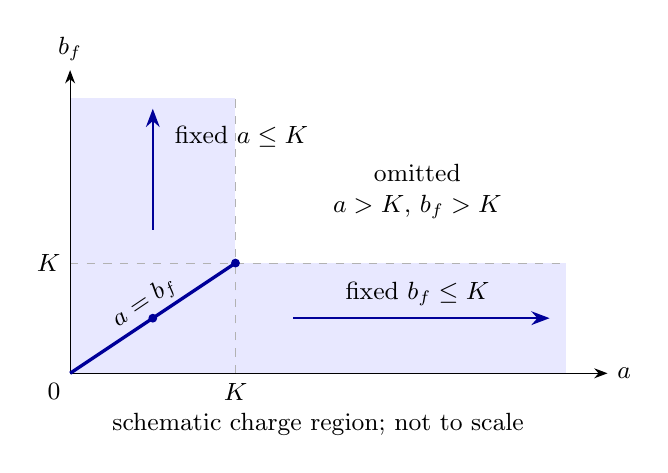
\begin{tikzpicture}[x=1.05cm,y=0.70cm,>=Stealth,font=\small]
  \fill[blue!9] (0,0) rectangle (2,5);
  \fill[blue!9] (2,0) rectangle (6,2);
  \draw[gray!60,dashed] (2,0) -- (2,5);
  \draw[gray!60,dashed] (0,2) -- (6,2);
  \draw[->] (0,0) -- (6.5,0) node[right] {$a$};
  \draw[->] (0,0) -- (0,5.5) node[above] {$b_f$};
  \node[below left] at (0,0) {$0$};
  \node[below] at (2,0) {$K$};
  \node[left] at (0,2) {$K$};
  \draw[blue!60!black,very thick] (0,0) -- (2,2);
  \fill[blue!60!black] (1,1) circle (1.6pt);
  \fill[blue!60!black] (2,2) circle (1.6pt);
  \node[rotate=34,anchor=south] at (1.05,0.96) {$a=b_f$};
  \draw[->,thick,blue!60!black] (1,2.6) -- (1,4.8);
  \node[align=left,anchor=west] at (1.15,4.3) {fixed $a\le K$};
  \draw[->,thick,blue!60!black] (2.7,1) -- (5.8,1);
  \node[anchor=south] at (4.2,1.05) {fixed $b_f\le K$};
  \node[align=center] at (4.2,3.3) {omitted\\$a>K$, $b_f>K$};
  \node[anchor=north] at (3,-0.55) {schematic charge region; not to scale};
\end{tikzpicture}
\caption{A finite request retains $\min(a,b_f)\le K$, a finite union
of convergent fixed-side tails; its balanced part is finite.
The excluded region has both charges larger than $K$, so its
monomials carry the corresponding power of the transfer charge on
the actual passage.  Not every schematic lattice position need occur.
No coefficient bound uniform in the fixed side, or convergence of
the unrestricted mixed series, is asserted.}
\label{fig:retained-charges}
\end{figure}


\begin{lemma}[Slow coefficients on a common fast radius]\label{lem:additive-slow}
The graph, fiber transformation in its convergent state-disk norm, and
$b$ in (A) are bounded on the lateral domains.  The transformation is
close to the identity and has a regular inverse on a smaller disk
covering the inputs.  In (B), for each fixed $m$ the full $H$ tail
converges on one fixed fast radius; the corresponding assertion holds
with the sides interchanged.  These radii cover the actual fast
amplitudes with fixed slack and do not decrease with $m,n$, or $K$.
State, profile, and spatial neighborhoods have common positive remaining
margins.  The finite balanced lists have the same estimates.

Each such fixed request has a formal series in $h=1/w$, whose coefficients
are analytic in independent profile and ordinary arguments on fixed
smaller polydisks and satisfy
\begin{equation}\label{eq:additive-Gevrey}
 \|c_j\|\le C^{j+1}j!.
\end{equation}
On padded interiors, for $1\le J\le c|w|$,
\begin{equation}\label{eq:additive-Gevrey-error}
 \left\|c(w)-\sum_{j<J}c_j(X)w^{-j}\right\|
       \le C^{J+1}J!|w|^{-J};
\end{equation}
a sufficiently small proportional optimal cutoff gives $O(e^{-c|w|})$.
For unscaled positive-profile coefficients
$\tau_j=\chi_jQ^{-r_j}$, so that $X_j=\tau_jw^{r_j}$,
the same estimates for $\partial_\tau^\alpha$ acquire the factor
$|w|^{r\cdot\alpha}$.  Fixed ordinary derivatives are allowed.
Neighboring anchor choices of size comparable to $|Q|$ differ by
$O(e^{-c|Q|})$ on the common working interior, including at its inner
radius, with fixed polynomial derivative losses allowed.
At $\tau=0$ the finite positive-profile jets have canonical
infinite-anchor determinations with these estimates.
\end{lemma}

\begin{proof}
We first construct the actual coefficients on the lateral domains.
For (B), this is an induction in the left degree: at each step a finite
list of opposite degrees precedes one convergent high opposite tail.
A fixed request involves only finitely many such blocks.
We then obtain formal Gevrey bounds and compare their optimal truncations
with those actual coefficients.  The common domain choices are made
before this second induction, so its slow order can grow without
exhausting the margins.  Weighted derivatives and anchor comparisons
complete the proof.  Throughout, a common fast radius does not assert
coefficient bounds uniform in the left degree or convergence when both
fast degrees grow.

\emph{1. Convergent lateral coefficients.}

For $\mathcal L=\partial_w+\Delta(1+Z)+\kappa/w$, its zero-data
inverse has kernel
\begin{equation}\label{eq:additive-kernel}
 \exp[-\Delta(w-w')-\Delta\gamma\log(w/w')]
                    (w'/w)^\kappa.
\end{equation}
On an admissible monotone graph, $|\gamma/w|\le C|\delta|$.
If $|\kappa/\Delta|$ is universally bounded, small $\delta$ and
large fixed $q_*$ give kernel decay $Ce^{-c|\Delta||x-x'|}$
and inverse norm $C/|\Delta|$.  For a fixed exceptional pair the last
factor in \eqref{eq:additive-kernel} is bounded by
$C(1+|x-x'|)^{C_\kappa}$: the log angle is bounded and both radii are
bounded below.  Its exponential moment is finite.  Thus exceptional
pairs only change their constants; they do not require increasing
$q_*$ as the requested charge order increases.  Fixed profile weights
commute through the kernel with the same polynomial ratio estimate.

The graph equation is a contraction on a small sup-norm ball, because
$g=O(X)$ and its state derivative is $O(X)$.
For the fiber coefficients use the norm $\sum_{m\ge2}R^m\|t_m\|$ on a
small state disk.  The inverse gains $C/(m-1)$, compensating the degree
factor in analytic composition.  More explicitly, expand $g$ in a disk
strictly inside its analytic state box, majorize its coefficients by
the corresponding absolutely convergent positive Taylor series, and
solve successive coefficient truncations in a small ball.  The
$1/w$ multiplier is at most $C/q_*$; terms containing $mb/w$ have
uniformly small norm after division by $m-1$.  The majorant map has
small Lipschitz constant.  Its bound is independent of the truncation,
so the increasing sums converge, and Cauchy on a smaller state disk
makes $T_u-1$ small.  The inverse follows by contraction.

The pure $E$ and pure $H$ transformations in (B) have no drift
interaction.  Their right sides have a fast factor.  A Taylor majorant
on small fixed fast disks and a larger state disk is therefore a
contraction with small state derivative.  Now fix $m\ne0$ and write
\[
 T_m(H)=\sum_n t_{mn}H^n,\qquad
 A_0(H)=G_z(X,0,H,u+T_0(H)).
\]
Here $A_0(0)=0$.  At the current left order, the unknown $T_m$ enters
$G$ only as the linear convolution $A_0T_m$; every nonlinear remainder
uses smaller componentwise left orders.  Also $\mathcal C_{0,*}=0$,
so $\partial_ut\,\mathcal C$ never differentiates the current unknown
$T_m$.  Current balanced coefficients multiply only
$\partial_uT_0$; they form a finite list with $b\cdot n=a\cdot m$ and
are determined in increasing opposite degree before the high tail.

Choose a fixed fast radius $\rho$ strictly inside the pure-side radius
and use the weighted absolute coefficient norm on a chosen lateral
domain $\Omega$ and state disk $D_R=\{|u-u_c|<R\}$,
\begin{equation}\label{eq:additive-tail-norm}
 \|F\|_{\rho,R}=\sum_n\rho^{|n|}
             \sup_{w\in\Omega,\,|u-u_c|<R}|F_n(w,u)|.
\end{equation}
It is a Banach algebra without any loss of $\rho$.  To make the uniformity
explicit, put $a_{\min}=\min_s a_s$, $b_{\min}=\min_s b_s$,
$\beta_{\max}=\max_s|\beta_s|$, and
$\nu_{\max}=\max_s|\nu_s|$.  For
$N=N(m)\ge\max(1,2a/b_{\min})$ and $|n|>N$,
\[
 \Delta_{mn}\ge\tfrac12 b_{\min}|n|,\qquad
 |\kappa_{mn}/\Delta_{mn}|
    \le\beta_{\max}/a_{\min}+2\nu_{\max}/b_{\min}.
\]
In particular the high-tail kernel constants and the initial choice of
$q_*$ are independent of $m$.
After solving the finite initial list, its high tail $U$ satisfies
\begin{equation}\label{eq:additive-tail-contraction}
 U=\mathcal L_m^{-1}\Pi_{>N}(A_0U+F_m),\qquad
 \|\mathcal L_m^{-1}\Pi_{>N}F\|_{\rho,R}
      \le\frac{C_0}{N}\|F\|_{\rho,R}.
\end{equation}
The forcing $F_m$ consists entirely of known lower-left tails and the
finite initial list.  Taking $N>2C_0\|A_0\|_{\rho,R}$ yields
\[
 \|U\|_{\rho,R}\le(2C_0/N)\|F_m\|_{\rho,R}.
\]
This proves convergence on the same $\rho$ at every left order.
Large mixed coefficients do not violate the field box: their Taylor
construction is coefficientwise in the left variables about the small
pure-side base, rather than an evaluation of the whole mixed series.

\emph{2. Domains shared by all slow orders.}
The preceding induction gives the actual coefficients on a common fast
radius.  To compare them with formal slow expansions, we must also reserve
state, profile, and spatial room at every finite dependency step.  We make
those choices now, independently of the slow truncation order.  Fix a
finite coefficient and derivative request and close its dependencies
under smaller left orders, opposite initial indices, and lower jets.
Choose positive limiting profile and state radii $x_\infty,R_\infty$
strictly inside the pure-side construction, and a spatial padding
$\zeta_\infty$ strictly inside the available geometric room.  Choose
$\eta_k=c_1/(k+1)^2$, $k\ge1$, with total sum smaller than each of the
three available margins, and define
\begin{equation}\label{eq:additive-reservoirs}
 x_k=x_\infty+\sum_{h>k}\eta_h,\qquad
 R_k=R_\infty+\sum_{h>k}\eta_h,\qquad
 \zeta_k=\zeta_\infty-\sum_{h>k}\eta_h.
\end{equation}
The fixed amplitudes can be chosen so that actual profiles lie in
$|X|<x_\infty/2$ on the whole larger lateral domain.  State coefficient
functions at degree $k$ are constructed on
$|u-u_c|<R_k+\eta_k/4$ and are estimated, with arbitrary fixed state
jets, on $D_{R_k}$.  Lower-left coefficients are available at $R_{k-1}$;
in particular, for a fixed derivative order $d$,
\begin{equation}\label{eq:additive-inherited-Cauchy}
 \|\partial_u^d F_{m'}\|_{\rho,R_k+\eta_k/4}
 \le d!\left(\frac{4}{3\eta_k}\right)^d
             \|F_{m'}\|_{\rho,R_{k-1}},\qquad |m'|<k.
\end{equation}
The same estimate applies to predecessor differences in a comparison.
The current unknown is never differentiated in $u$ by its defining
equation.  The reserved $\eta_k/4$ gives its requested output state
derivatives after it has been constructed.

There are finitely many left indices of degree $k$.  Take a common
threshold $N_k$ for their high opposite tails, first larger than all
$2a/b_{\min}$ and then large enough to absorb the pure multiplier in
both the actual and formal norms below.  List the finite opposite
degrees in increasing order, followed by the high tail.  Include the
finitely many lower-jet comparison steps required for the present
request.  Call the number of resulting steps $s_k$.  Each infinite
same-sign tail counts as one step, not as infinitely many indices.
For $0\le v\le s_k$, use the spatial domains
\begin{equation}\label{eq:additive-spatial-schedule}
 \Omega_{k,v}=\left\{w\in\Omega_B^\pm:
  \dist(w,\partial\Omega_B^\pm)>
   \left(\zeta_{k-1}+\frac{v\eta_k}{s_k}\right)|w|\right\}.
\end{equation}
These are estimates on restrictions of the same actual coefficient
functions, not newly prescribed boundary data.  A target in
$\Omega_{k,v}$ has, in either horizontal direction, a segment of length
$b_k|w|$ contained in $\Omega_{k,v-1}$, with all radii comparable to
$|w|$, where one may take
$b_k=\eta_k/[8s_k(1+\zeta_\infty)]$.
This follows from the $1$-Lipschitz property of distance and of modulus.
All orders end on the same positive remaining profile/state margins
and on a spatial padding less than $\zeta_\infty$.  Increasing a finite
jet request changes $s_k,b_k$ and the constants, without changing those
limiting margins or the fast radius $\rho$.

\emph{3. Formal Gevrey bounds.}
On the domains just chosen, write
\[
 \partial_w=h(D_X-h\partial_h),\qquad
 D_X=\sum_j r_jX_j\partial_{X_j}.
\]
Divide the recursions by their nonzero diagonal at $h=0$, a nonzero
integer charge times $1+Z$.  Work modulo $h^{J+1}$, $J\ge1$, put
$\theta=\varepsilon_k/(J+1)$, and, for $0\le j\le J$, set
\begin{align}
 x_{k,j}^{(J)}&=x_k+\frac{\eta_k}{4}
       +\frac{\eta_k}{4}\left(1-\frac{j}{J+1}\right),
             \label{eq:additive-formal-disks}\\
 \|F\|_{k,J}&=\sum_{j=0}^J\theta^j\sum_n\rho^{|n|}
     \sup_{\substack{|X|<x_{k,j}^{(J)}\\
                     |u-u_c|<R_k+\eta_k/4}}|F_{jn}(X,u)|.
             \label{eq:additive-formal-norm}
\end{align}
For a finite scalar coefficient omit the sum over $n$.  Every current
profile disk lies at least $\eta_k/2$ inside the predecessor target
disk $|X|<x_{k-1}$, and at least $\eta_k/4$ outside the current target
disk $|X|<x_k$.  Thus there is both inherited room and fixed residual
room.  In a product the target disk at degree $a+b$ lies in both input
disks, so this norm is an algebra.  The disk gap for a single slow
degree is $\eta_k/[4(J+1)]$.  Cauchy's inequality and the factor
$\theta$ give
\begin{equation}\label{eq:additive-truncated-operators}
 \|hD_X\|\le C\varepsilon_k/\eta_k,\qquad
 \|h^2\partial_h\|\le C\varepsilon_k,
 \qquad\|\Delta^{-1}h\kappa\|\le C\varepsilon_k
\end{equation}
on the high tail; the finite exceptional list has its own constants.

To spell out the induction inequality, let $M_{k,v}^{(J)}$ denote the
norm of the current formal coefficient block, and let $M_{\prec}^{(J)}$
be the maximum of the norms already constructed that enter its
forcing.  Fixed left-degree extraction of $G$ is a finite Taylor
calculation about the pure-side base.  Its terms have bounded analytic
multilinear coefficients and finitely many predecessor factors.
The drift contributes products with a lower-left state derivative,
bounded by \eqref{eq:additive-inherited-Cauchy}.  Hence there are fixed
$D_k,d_k$ and constants $C_{k,v}$, independent of $J$, for which that
forcing is bounded by
\[
 \Phi_{k,v}(M_{\prec}^{(J)})
 :=C_{k,v}(1+\eta_k^{-d_k})(1+M_{\prec}^{(J)})^{D_k}.
\]
The exponents are finite because the left Taylor degree and the jet
request are finite; no bound as $k$ increases is required.  Dividing
by the diagonal, and moving only its slow differential correction to
the right, gives for an exceptional coefficient
\begin{equation}\label{eq:additive-formal-induction}
 M_{k,v}^{(J)}\le
 \Phi_{k,v}(M_{\prec}^{(J)})+
 C_{k,v}\varepsilon_k(1+\eta_k^{-1})M_{k,v}^{(J)}.
\end{equation}
For the high tail it gives the same inequality with the last
coefficient replaced by
\begin{equation}\label{eq:additive-formal-tail-induction}
 \frac{C\,M_A}{N_k}
       +C_k\varepsilon_k(1+\eta_k^{-1}),
\end{equation}
where $M_A$ bounds the pure-side multiplier in its larger-disk formal
norm, uniformly in $J$.  Balanced blocks satisfy the forcing inequality
without a current unknown on the right.  The graph, fiber disk norm,
and pure-side blocks obey the corresponding analytic majorant
inequality with their already chosen small Lipschitz constant; their
slow differential correction has the same bound.

First choose $N_k$ to make $CM_A/N_k\le1/4$.  Induct through the finite
list, taking $\varepsilon_k$ smaller than every preceding admissible
choice and so small that all the differential coefficients in
\eqref{eq:additive-formal-induction}--\eqref{eq:additive-formal-tail-induction}
are at most $1/4$.  Absorption yields
$M_{k,v}^{(J)}\le2\Phi_{k,v}(M_{\prec}^{(J)})$.
Its finite recursion supplies a bound independent of $J$.
Shrinking $\varepsilon_k$ only decreases predecessor norms, so it
does not invalidate a prior bound.  This proves the simultaneous
formal induction on the specified disks.  At $J=j$ it implies
\[
 \|c_j\|\le C_0((j+1)/\varepsilon_k)^j
          \le C^{j+1}j!,
\]
using $j^j\le e^jj!$.  Fixed formal profile or state derivatives are
taken on the reserved target disks and change only their fixed
Cauchy constants.

\emph{4. Comparison with optimal truncations.}
The formal norm now bounds the substitution residual.  To turn this
into an estimate for the actual coefficient, we use a last horizontal
comparison segment of
length $\delta_m|w|$ in the appropriate damping direction, lying in
a padded interior, with radii comparable to $|w|$.  Substitute the
formal polynomial with $J$ a small multiple of $|w|$.  Test that
polynomial and all analytic operations at a dummy $h$ radius larger
than the actual $|1/w|$ by a fixed factor.  Formal cancellation below
degree $J$ and the just proved sum bound give an exponentially small
residual in the norm appropriate to its diagonal.  A diagonal or
$\kappa$ factor can contribute $1+|n|$ to this residual.  More precisely
introduce the forcing norm
\[
 \|F\|_{\rho,R,-1}
   =\sum_n\frac{\rho^{|n|}}{1+|n|}
       \sup_{\Omega\times D_R}|F_n|.
\]
The residual is $Ce^{-c|w|}$ in this norm, whereas the inverse maps
this forcing space boundedly into \eqref{eq:additive-tail-norm}.
Indeed apply the inverse coefficientwise before summing: on the high tail
\begin{equation}\label{eq:additive-index-cancellation}
 (1+|n|)/|\Delta_{mn}|\le C.
\end{equation}
Thus there is no hidden fast-radius loss in this step.

Here is the actual comparison inequality, including its starting term.
For a target of modulus $R$, take the segment from
\eqref{eq:additive-spatial-schedule}, oriented in the current damping
direction and parametrized by real distance $t\in[0,L]$, $L=b_kR$.
Let $E$ be actual coefficient minus its common formal polynomial.
The actual coefficients are uniformly bounded by the preceding
Volterra construction, and the formal sum norm bounds that polynomial
on the segment.  Thus
$\sum_n\rho^{|n|}\sup_{D_{R_k}}|E_n(0)|\le B_{k,v}$,
with no dependence on $R$ or $J$.  Normalize by $R^{r\cdot\alpha}$
for a fixed positive-profile jet; moduli on this segment are comparable
to $R$, so the same assertion holds with a different fixed constant.

Use the coefficient-sum weighted norms
\begin{equation}\label{eq:additive-weighted-segment}
 \|E\|_\omega=\sum_n\rho^{|n|}
       \sup_{\substack{0\le t\le L\\u\in D_{R_k}}}
                   e^{\omega t}|E_n(t,u)|,
 \quad
 \|F\|_{\omega,-1}=\sum_n\frac{\rho^{|n|}}{1+|n|}
       \sup_{\substack{0\le t\le L\\u\in D_{R_k}}}
                   e^{\omega t}|F_n(t,u)|.
\end{equation}
The sum is outside each coefficient supremum.  This convention is
essential for the inverse from the weak forcing norm to the strong
norm; no interchange with a single supremum of the weak sum is used.
The high-tail kernels are bounded by
$Ce^{-\lambda(1+|n|)(t-s)}$.  For $0<\omega<\lambda/2$, coefficientwise
integration therefore gives a bounded map from the second norm to the
first, and a bound $C/N_k$ from the strong forcing norm to the first.
Finite exceptional kernels have bounds $C_{k,v}e^{-\lambda_{k,v}(t-s)}$
and the analogous scalar assertion for $\omega<\lambda_{k,v}/2$.

At a current high tail the difference equation has the form
$\mathcal L_mE=A_0E+F$, where $F$ is the formal substitution residual
plus predecessor differences.  Precisely, if $P_J$ is the current
polynomial, $A_J,F_J$ are the polynomial predecessor evaluations, and
$\mathcal R_J=\mathcal L_mP_J-A_JP_J-F_J$, then
\[
 F=(A_0-A_J)P_J+(F_{\rm actual}-F_J)-\mathcal R_J.
\]
The finite Taylor operations defining
the forcing are Lipschitz on their bounded coefficient balls; their
Lipschitz constants are finite derivatives of $\Phi_{k,v}$.
Inherited state derivatives use
\eqref{eq:additive-inherited-Cauchy}.  Consequently, by the previous
comparison stages and the residual estimate, on this whole segment
\[
 \|F\|_{0,-1}\le C_{k,v}e^{-a_{k,v}R}
\]
for some $a_{k,v}>0$.  Predecessors may all use the current smaller
proportional cutoff: subtracting the finite Gevrey tails preserves
an exponential error.  In the exceptional list there is no current
multiplier; for a graph or pure side its place is taken by the small
linearized coefficient.  Variation of constants now gives
\begin{equation}\label{eq:additive-actual-induction}
 \|E\|_\omega\le C_{k,v}B_{k,v}
       +\tfrac12\|E\|_\omega
       +C_{k,v}e^{\omega L-a_{k,v}R}.
\end{equation}
The factor $1/2$ is ensured by the tail threshold, or the original
pure-side smallness, after the harmless weighted-kernel change.
Choose additionally $\omega b_k\le a_{k,v}/2$.  At the endpoint this
proves the explicit estimate
\begin{equation}\label{eq:additive-actual-endpoint}
 \|E(L)\|_{\rho,R_k}\le
 C_{k,v}\bigl(B_{k,v}e^{-\omega b_kR}+e^{-a_{k,v}R}\bigr).
\end{equation}
It has a positive exponential rate at every finite step.  Alternating
signs use the successive domains in
\eqref{eq:additive-spatial-schedule}; one infinite high tail uses one
segment, with its whole coefficient sum.  Thus the finite induction
closes without any fast-radius loss or exhaustion of the prescribed
state, profile, or spatial margins.  This proves the optimal error;
subtracting the omitted Gevrey terms proves
\eqref{eq:additive-Gevrey-error} at smaller orders.  Remaining bounded
radii for a fixed $J$ are absorbed in its constant.

\emph{5. Weighted profile derivatives.}
Differentiating at fixed anchors in $\tau$ gives polynomial weights
$w^{r\cdot\alpha}$.  The highest derivative of a graph or pure side
has the same small linearization, and the highest derivative of a high
tail has the same absorbable convolution.  The other terms use lower
derivatives.  Apply the unweighted resolvent first and then commute a
fixed polynomial weight through its decaying kernel; the resulting
constant is an exponential moment
$\int_0^\infty e^{-ct}(1+t)^{C_\alpha}\dd t<\infty$.
One need not demand that this weighted constant remain small.  More
explicitly, $A_0(0)=0$ means that each convolution step increases the
opposite degree.  In the iterated Volterra resolvent, a column starting
at degree $n_0$ is therefore bounded in weighted absolute coefficient
sum by
\[
 C e^{-\lambda(1+|n_0|)t}
       \sum_{v\ge0}\frac{(CM_A t)^v}{v!}
 \le C e^{-\lambda'(1+|n_0|)t},
\]
after the chosen high-tail threshold is increased once, if necessary.
For a pure side the same inequality follows from its original
smallness.  Along a monotone path, the ratio of either endpoint modulus
to the other is at most $1+Ct/q_*$.  Multiplying this resolved kernel
by a fixed power of that ratio gives a finite exponential moment and
still an inverse bound $C_\alpha/(1+|n_0|)$.  Thus the global weighted
jet bounds, and in particular the normalized starting bounds in
\eqref{eq:additive-actual-induction}, follow before any jet comparison.
Adding the finitely many lower-jet comparisons to the spatial schedule
then proves the differentiated errors with the same remaining domains.

\emph{6. Anchor comparison and limiting jets.}
Compare neighboring anchors using a common inner polygon with
horizontal extremes fixed large multiples of $|Q|$, leaving the
working target region $|\Re w|\le C_1|Q|$ strictly inside.  At each of
the finitely many comparison steps divide its allotted horizontal
margin by $s_k$ and choose a starting line on the appropriate side.
The monotone graphs used in constructing the lateral domain connect
that line to every target, with bounded slope and real distance at
least $b_{k,v}'|Q|$, where $b_{k,v}'>0$.  These paths can pass above the
inner obstacle; they need not be horizontal across it.  Graph and
pure-side differences have homogeneous absorbable equations.  At a
later step the difference forcing is bounded by the derivative of the
same finite polynomial majorant times predecessor differences.
The weighted argument \eqref{eq:additive-actual-induction}, now with
$R=|Q|$, therefore gives
\[
 E_{k,v}\le C_{k,v}|Q|^{p_{k,v}}
 \left(e^{-\omega b_{k,v}'|Q|}
                 +\max_{\prec}E_{\prec}\right).
\]
Here $p_{k,v}$ accounts for the fixed jet weights on the whole path;
without such jets it can be zero.  Finite induction proves
$E_{k,v}\le C_{k,v}'e^{-c_{k,v}|Q|}$ with $c_{k,v}>0$.
The starting distance is of outer-scale size also when the target is
near $q$, so the estimate holds uniformly down to the inner radius.
At $\tau=0$
positive-growth profiles disappear; their finite jets solve equations
with fixed polynomial weights.  Compare consecutive dyadic outer
anchors and sum their exponentially small differences on each fixed
interior.  The locally uniform limit gives the asserted analytic,
canonically normalized infinite-anchor jets and all their estimates.
\end{proof}

\subsection{Slow primitives and their normalization}

The linear coordinate in (A) needs a primitive $I$ satisfying
\begin{equation}\label{eq:additive-I}
 D I=b(w),\qquad D=w\partial_w.
\end{equation}
In (B), every balanced drift term in
\eqref{eq:additive-balanced-P} has positive degree in $P$.  A fixed
charge coefficient of its flow therefore uses only finitely many
iterations of the integral equation.  These give nested integrals of
entries $w^{d_e}c_e(w)$ in logarithmic time, with fixed rational $d_e$.
The factor changing $\dd w$ to $\dd w/w$ is included in $d_e$.
The functions $c_e$ are balanced slow coefficients or fixed derivatives
in an ordinary state argument, which is held independent at this step.
For each required word use a strictly upper triangular matrix having
its successive entries on the first upper diagonal.  A unit upper
triangular fundamental matrix $Y$ has entries satisfying
\begin{equation}\label{eq:additive-word}
 D Y_{\mathbf e}=w^{d_e}c_e(w)Y_{\rm tail},\qquad
 Y_\emptyset=1.
\end{equation}
Include all consecutive subwords.  Its transfer is $Y(p)Y(q)^{-1}$,
a polynomial in these finitely many entries.  This representation uses
no exponential bound on an unrestricted matrix flow over a long
logarithmic interval.

\begin{lemma}[Normalized slow primitives]\label{lem:additive-primitives}
There are particular formal primitives
\begin{equation}\label{eq:additive-formal-word}
 \widehat Y_{\mathbf e}
 =w^{d_{\mathbf e}}\sum_{j\ge0}w^{-j}B_{\mathbf e,j}(X,L),
 \qquad d_{\mathbf e}=\sum_{e\in\mathbf e}d_e,
 \qquad L=\log(w/q),
\end{equation}
where $B_{\mathbf e,j}$ is polynomial in $L$ of degree at most the
word length and its analytic coefficient norm is at most $C^{j+1}j!$.
The analogous assertion holds for $\widehat I$ with $d=0$ and length one.

Normalize the actual primitives by a sufficiently small proportional
optimal truncation at a positive $w_*$ comparable to $|Q|$, in the common
padded interior.  Then $I$ is bounded on the needed paths, and on a
matching outer ray the normalized outer values are approximated by
their formal optimal truncations with error $O(e^{-c|Q|})$.
The inner kernels
\begin{equation}\label{eq:additive-inner-kernels}
 I(q),\qquad q^{-d_{\mathbf e}}Y_{\mathbf e}(q)
\end{equation}
are bounded, have Gevrey expansions in $1/q$ obtained by setting $L=0$
in \eqref{eq:additive-formal-word}, and obey the differentiated estimates
of Lemma~\ref{lem:additive-slow}.  In particular a positive-profile jet
of order $\alpha$ is bounded after division by $q^{r\cdot\alpha}$.
Neighboring finite normalizations change these kernels by
$O(e^{-c|Q|})$, allowing fixed polynomial losses.

At zero positive profiles there are canonical infinite-anchor primitive
jets.  Their normalized inner values have the same Gevrey estimates.
For each fixed jet and each fixed $N$, finite and infinite normalized
jets differ by $O_N(|Q|^{-N})$.  This last assertion is power accuracy,
and does not claim exponential accuracy in $|Q|$.
\end{lemma}

\begin{proof}
\emph{1. Formal primitives and outer normalization.}
Multiply the already constructed formal series and argue by word
length.  The factorial inequality
$\sum_{k=0}^j k!(j-k)!\le Cj!$ preserves the asserted Gevrey order.
On a profile monomial $X^\mu$ the primitive operation is inversion of
\begin{equation}\label{eq:additive-resonance-operator}
 r\cdot\mu+d_{\mathbf e}-j+\partial_L.
\end{equation}
All its nonzero constant parts have absolute value at least $1/D_0$
for one fixed common rational denominator $D_0$.  On polynomials of
degree at most $s$, for $c\ne0$ its inverse is the finite expression
\[
 (c+\partial_L)^{-1}F
       =\sum_{k=0}^{s}(-1)^kc^{-k-1}\partial_L^kF.
\]
At $c=0$ integrate in $L$, choosing zero integration constant.  These
operators have bounds depending only on $s,D_0$.  Use absolutely
convergent profile coefficient norms on smaller disks to sum them.
Induction gives \eqref{eq:additive-formal-word} with degree at most
the word length.  In particular the formal choices have no undetermined
constants.

Freeze $w_*$ and the truncation order on each modulus choice.  Define
the actual triangular solution by those truncated values at $w_*$;
define $I$ in the same way.  For its leading coefficient,
$\widehat b_0=g_v(X,0)$ has no constant profile monomial.  A resonant
monomial at slow order zero must therefore involve both positive and
negative profile weights.  If the total positive weight is $\rho>0$,
its evaluation contains $(q/Q)^\rho$, and these positive weights have
a fixed positive rational minimum.  Thus the coefficient of $L$ at
order zero pays $\log(w_*/q)$.  Higher slow orders carry at least
$w_*^{-1}$, which pays this logarithm as well.  The normalized value of
$I$ at $w_*$ is bounded.  Since $b=O(X)$ on the actual graph, integrating
along radial and bounded-angle arc paths gives a bounded variation by
the nonzero profile powers, as in \eqref{eq:additive-slow-integral}.
This proves the boundedness needed for its later exponential.

If $p$ lies on the matching $Q$ ray, connect it to $w_*$ using paths with
all radii comparable to $|Q|$.  A common smaller optimal truncation
has exponentially small substitution residual, by
Lemma~\ref{lem:additive-slow}.  Triangular integration loses only fixed
powers and fixed-degree logarithms; these are absorbed by decreasing
the exponential constant.  This proves the outer endpoint assertion.
No actual evaluation of $I(p)$ at a multiply wound $Q$ is required.

\emph{2. Uniform propagation to the inner endpoint.}
The outer normalization alone does not bound the inner kernels when
$|Q|/|q|$ diverges.  We compare the actual and formal primitives along
the full inward path.  The triangular equations preserve their explicit
power weights, and a sufficiently high slow order makes those weights
integrable with constants independent of the endpoint ratio.

Fix the finite word and jet list, closed under
consecutive subwords and lower jets.  Put $q_0=|q|$, $R=w_*$,
$p_\alpha=r\cdot\alpha$, $\beta_{v,\alpha}=d_v+p_\alpha$, and
$\ell(t)=1+\log(t/q_0)$.  Fixed ordinary derivatives may be included
in the jet list with weight zero.  First compare on the radial part
$q_0\le t\le R$, and then on a bounded-angle arc to $q$.
For a word $v=e\,v'$ define
\[
 P_v^J(w)=w^{d_v}\sum_{j<J}B_{v,j}(X,L)w^{-j},\qquad
 c_e^{<L_0}(w)=\sum_{a<L_0}c_{e,a}(X)w^{-a}.
\]
Formal coefficient comparison gives the exact finite identity
\[
 DP_v^J=w^{d_v}\sum_{a+b<J}c_{e,a}B_{v',b}w^{-a-b}.
\]
Consequently the local substitution residual is exactly
\begin{equation}\label{eq:additive-primitive-residual-identity}
 \mathcal R_v^J:=w^{d_e}c_eP_{v'}^J-DP_v^J
 =w^{d_v}\sum_{b<J}w^{-b}B_{v',b}
                  (c_e-c_e^{<J-b}).
\end{equation}
Thus its estimate does not presuppose an estimate for an actual
primitive remainder.  On the fixed smaller profile disks the formal
coefficient bounds and Cauchy's inequality give
\[
 |\partial_\tau^\eta B_{v',b}|
 \le A_\eta C_0^{b+1}b!\,|w|^{p_\eta}\ell(|w|)^S,
\]
with one fixed $S$ covering all log degrees in the request.
Lemma~\ref{lem:additive-slow} gives, for $1\le L_0\le c|w|$,
\[
 |\partial_\tau^\eta(c_e-c_e^{<L_0})|
 \le A_\eta C_0^{L_0+1}L_0!\,|w|^{p_\eta-L_0}.
\]
The derivatives are at fixed $q,w_*$ and other independent arguments,
so they commute with $D$.  After Leibniz differentiation of
\eqref{eq:additive-primitive-residual-identity}, each term has power
$d_v-b+p_{\alpha-\eta}+p_\eta-(J-b)=\beta_{v,\alpha}-J$.
Using $\sum_{b<J}b!(J-b)!\le3J!$ and absorbing the finitely many jet
binomial factors proves
\begin{equation}\label{eq:additive-primitive-residual}
 |\partial_\tau^\alpha\mathcal R_v^J(w)|
 \le C_\alpha^{J+1}J!\,
       |w|^{\beta_{v,\alpha}-J}\ell(|w|)^S.
\end{equation}

The initial normalization tail has the very same weight.  Indeed
choose $K_R=\lfloor\varepsilon R\rfloor$ on larger parameter disks
such that $C_0K_R/R\le\theta<1$.  Fixed derivatives cost Cauchy
prefactors, while the coefficient-growth constant $C_0$ can be chosen
on those larger disks.  For $J\le cq_0\le K_R$, the geometric tail
estimate and $Y_v(R)=P_v^{K_R}(R)$ give
\begin{equation}\label{eq:additive-primitive-initial-tail}
 \left|\partial_\tau^\alpha(Y_v-P_v^J)(R)\right|
 \le\frac{A_\alpha}{1-\theta}C_0^{J+1}J!
        R^{\beta_{v,\alpha}-J}\ell(R)^S.
\end{equation}
The anchors and integer orders are frozen in these derivatives.

Write $E_{v,\alpha}^J=\partial_\tau^\alpha(Y_v-P_v^J)$.
Its differentiated equation is
\begin{equation}\label{eq:additive-primitive-error-system}
 D E_{v,\alpha}^J
 =w^{d_e}\sum_{\eta\le\alpha}\binom{\alpha}{\eta}
       (\partial_\tau^\eta c_e)E_{v',\alpha-\eta}^J
                   +\partial_\tau^\alpha\mathcal R_v^J.
\end{equation}
Since $|\partial_\tau^\eta c_e|\le C_\eta|w|^{p_\eta}$,
the power of each predecessor error on the right is exactly
$d_e+p_\eta+\beta_{v',\alpha-\eta}-J
=\beta_{v,\alpha}-J$.
Choose $J>1+\max_{v,\alpha}\beta_{v,\alpha}$, the maximum being over
the entire finite system.  For any such $\beta$ and $q_0\le t\le R$,
\begin{equation}\label{eq:additive-inward-integral}
 R^{\beta-J}\ell(R)^S+
 \int_t^R s^{\beta-J}\ell(s)^S\,\frac{\dd s}{s}
 \le C_S t^{\beta-J}\ell(t)^S.
\end{equation}
For the integral put $s=te^x$, use
$\ell(te^x)\le\ell(t)(1+x)$, and bound
$\int_0^\infty e^{-x}(1+x)^S\dd x$.
The boundary term follows from the bounded supremum of the same
function.  Both bounds are uniform in $t,R,q_0,J$; in particular the
initial tail cannot accumulate a factor depending on $R/q_0$.

For explicit triangular bookkeeping, let
\[
 X_{v,\alpha}^J=
 \sup_{q_0\le t\le R}
  \frac{|E_{v,\alpha}^J(t)|}
       {C_0^{J+1}J!t^{\beta_{v,\alpha}-J}\ell(t)^S}.
\]
Equations~\eqref{eq:additive-primitive-residual}--\eqref{eq:additive-inward-integral}
give
\begin{equation}\label{eq:additive-primitive-triangular-bound}
 X_{v,\alpha}^J\le B_{v,\alpha}
       +C_S\sum_{\eta\le\alpha}B_{e,\eta}
                         X_{v',\alpha-\eta}^J,
\end{equation}
after choosing the common $C_0$ to dominate the residual constants.
All $B$'s depend only on the fixed finite request and domain margins.
The right side contains strictly shorter words.  Finite triangular
induction bounds every $X_{v,\alpha}^J$ independently of $J,R,q_0$.
The bounded-angle arc has radius comparable to $q_0$ and bounded lifted
logarithm; integrating the same finite triangular system there changes
only these constants.  At $w=q$, divide by
$q^{d_v+p_\alpha}$ to obtain $C^{J+1}J!q_0^{-J}$.

To cover all requested orders $J\ge1$, choose a fixed integer
$B>1+\max_{v,\alpha}\beta_{v,\alpha}$ and first make the comparison
at $J+B$.  Decrease the target proportional constant so that
$J+B\le c_0q_0$ on the unbounded range.  The apparent extra factorial
is canceled by the extra radius power:
\begin{equation}\label{eq:additive-fixed-J-shift}
 \frac{(J+B)!}{J!}\,q_0^{-B}
       =\prod_{s=1}^{B}\frac{J+s}{q_0}\le c_0^B.
\end{equation}
Add back the fixed $B$ formal terms of degrees $J$ through $J+B-1$.
Their Gevrey bounds give the same $C^{J+1}J!q_0^{-J}$ estimate, with
an enlarged constant.  The remaining bounded range of $q_0$ is handled
by first integrating down to a fixed radius above this threshold and
then over the remaining compact radial interval and arc.  There are
only finitely many allowed $J$ on that range, and $q_0\ge q_*>1$;
all constants are finite and uniform there.  This changes no original
smallness condition or initial $q_*$.  The case $I$ is the length-one
version of the same calculation.

\emph{3. Finite and infinite normalizations.}
For two neighboring finite normalizations compare first near their
outer normalization points.  Their formal optimal values and the
nonprimitive coefficients differ by $O(e^{-c|Q|})$.
Propagate inward using the triangular difference equations.  Every
word and fixed jet loses at most a fixed power of $|Q|$, since $q$ is
bounded below, so the inner difference remains exponentially small.

At $\tau=0$ use the canonical nonprimitive infinite-anchor jets from
Lemma~\ref{lem:additive-slow}.  Subtract a differentiated formal
truncation of sufficiently high fixed order $J$ and solve the residual
equations by integration from positive-real infinity, then by an
interior arc when required.  Convergence follows from
\eqref{eq:additive-inward-integral}.  Indeed a fixed derivative
$\partial_\tau^\alpha$ at zero selects exactly the positive-profile
multi-degree $\alpha$; all remaining profile powers are negative.
Its $j$th formal term is therefore bounded by
$C_{\alpha,j}|w|^{d_{\mathbf e}+r\cdot\alpha-j}
(1+\log(|w|/|q|))^s$.  Taking $J$ beyond all these fixed power costs
makes the subsequently omitted terms tend to zero at infinity.
Increasing $J$ gives the same
solution: the difference solves the homogeneous differentiated
triangular recursion, and its first nonzero entry is constant with
limit zero at infinity; inductively every entry is zero.  The same
construction at $J\le c|q|$ gives its Gevrey estimate.  Locally uniform
convergence gives analytic parameter germs.  At $w_*$ compare this
infinite solution and the finite normalization at any sufficiently
large fixed $J$.  Their difference is smaller than any prescribed
power of $|Q|^{-1}$, after allowing the fixed polynomial/logarithmic
losses.  Propagate to $q$ by the triangular equations, using the
exponentially small nonprimitive differences on the common path.
Choosing $J$ still larger pays the finite propagation losses and proves
the claimed $O_N(|Q|^{-N})$ estimate.
\end{proof}

In particular every bounded inner kernel $K$ just constructed admits a
finite Taylor expansion in the positive profiles at their current values
$\tau_j=\chi_jQ^{-r_j}$.  For a prescribed finite total Taylor degree
$N$, the integral Taylor remainder and the weighted jet bounds give
\begin{equation}\label{eq:additive-positive-Taylor}
 K(\tau)=\sum_{|\alpha|<N}\frac{\chi^\alpha}{\alpha!}
       (q/Q)^{r\cdot\alpha}\,
       \big[q^{-r\cdot\alpha}\partial_\tau^\alpha K(0)\big]
       +O\big((|q|/|Q|)^{r_{\min}N}\big),
\end{equation}
where $r_{\min}$ is the smallest positive profile weight.  For normalized
word kernels $K$ already includes $q^{-d_{\mathbf e}}$.  The Taylor
segment remains in the original independent profile boxes.
Replacing each finite zero-profile jet in this finite sum by its
infinite-anchor jet has arbitrary additional $|Q|^{-N'}$ accuracy.
If there are no positive profiles, the Taylor step is vacuous: retain
the single zeroth jet, with the same finite-to-infinite replacement.

\begin{lemma}[Bounded analytic Gevrey operations]\label{lem:additive-gevrey-operations}
Finite sums and products, analytic operations at bounded arguments with
fixed room in their convergence boxes, and regular inverses preserve
the normalized Gevrey and jet conclusions above.  For two independent
slow variables the resulting formal coefficients have bounds
\begin{equation}\label{eq:additive-rectangular}
 \|c_{ab}\|\le C^{a+b+1}a!b!.
\end{equation}
Rectangular optimal evaluation has separate errors
$O(e^{-c|Q_0|})+O(e^{-c|q_0|})$; changing only one optimal cutoff has
the accuracy of its own variable.  These conclusions remain uniform
when other bounded analytic arguments vary independently on smaller
fixed disks, and under fixed derivatives on those disks.
\end{lemma}

\begin{proof}
For finite budgets $J,N$, test the truncated inputs at dummy radii
$\varepsilon/(1+J)$ and $\varepsilon/(1+N)$.  Their nonconstant
increments are small in absolute coefficient norm and their constant
values stay strictly inside the analytic boxes.  Absolute Taylor
majorants therefore bound the output independently of $J,N$.
Extracting its $(a,b)$ coefficient with $J=a,N=b$ gives
\eqref{eq:additive-rectangular}, using $a^a\le e^aa!$ and the analogous
inequality for $b$.  For a regular inverse the analytic implicit
theorem applies on the dummy disks, uniformly on the smaller argument
boxes; the resulting majorant is bounded there.  Actual inverses and
their approximants differ by the residual times a bounded inverse
Jacobian, with the same finite differentiated bounds.

At sufficiently small proportional optimal orders the dummy radii
exceed the actual values by a fixed factor.  Terms omitted in one
variable have geometrically small absolute sum in that variable,
uniformly in the other dummy disk.  This gives the two separate
exponential errors and proves the assertion when one cutoff alone is
changed.  At a replacement of a bounded kernel, ordinary Cauchy bounds
first pay its actual error; the formal calculation is then performed
on the replacement.  Fixed derivatives use smaller disks with room.
For infinite-anchor jets the ordinary finite chain rule commutes with
the locally uniform limiting construction, so these are the same
canonical jets as those computed after the operation.
\end{proof}

\subsection{Finite expansions in the transfer charge}

For (A), use $T$ and $I$ from one fixed lateral construction at both
endpoints.  Exact conjugacy gives the terminal value
\begin{equation}\label{eq:additive-A-transfer}
 T\left(w_{\rm out},
 P e^{I(w_{\rm out})-I(w_{\rm in})}
                  T^{-1}(w_{\rm in},v_{\rm in})\right).
\end{equation}
The exact linear coordinate stays in its disk along the passage because
of homogeneous damping and the bounded small variation of
$\int b\,\dd w/w$.  Expanding the final evaluation of $T$ at $u=0$ to any fixed
degree in $P$ has a remainder $C_K|P|^{K+1}$.  Keep the actual bounded
inner kernels at $q$; replace outer kernels at $p$ by their optimal
formal values, with exponential error in $|Q|$.

Inside $e^{\pm I(p)}$ the formal logarithm deserves care.  Write its
coefficient at slow order $j$ as $R_j(X)L(p)$.  The order-zero
resonant sum is $(q/Q)^\rho$ times an analytic function of small
rational-power ratios, for some fixed $\rho>0$, by the opposing-profile
argument in Lemma~\ref{lem:additive-primitives}.  Treat
$(q/Q)^\rho L(p)$ as a small analytic argument.  For $j\ge1$ factor
one $Q^{-1}L(p)$ and shift the remaining slow series by one fixed
index, retaining the bounded factors of $p/Q$.  This avoids an
unbounded logarithm as an analytic input or a shift of Gevrey index
depending on the requested order.  Lemma~\ref{lem:additive-gevrey-operations}
then applies to the exponential.

For (B), retain the coefficients of
\eqref{eq:additive-balanced}--\eqref{eq:additive-imbalance} with
$\min(a,b_f)\le K$ and denote the result by
$t^{[K]},\mathcal C^{[K]}$.  The two fixed-side parts of $t^{[K]}$
are genuine analytic sums on their opposite fast disks, as established
for the region in Figure~\ref{fig:retained-charges}.
Their pure parts $t_L,t_R$ are small, including their state derivatives.  Although
the other coefficient norms may depend on $K$, every mixed retained
part evaluated on the actual integration polygon is
$O(C_K|Q|^{C_K}|P|)$, with every requested fixed state derivative.

Here is the estimate used repeatedly.  For an analytic fast sum all of
whose monomials have $\min(a,b_f)\ge k$, select from each side a
sub-multi-index of charge in $[k,k+c_*]$, where $c_*$ is the largest
generator weight.  Since both $\Re(A-q)$ and $\Re(Q-A)$ are
nonnegative, the exponential product of those selected factors is at
most $|P|^k$.  Their fixed rational powers cost at most
$C_k|Q|^{C_k}$.  The remaining fast factors sum on the common disk,
using the fixed amplitude slack.  Thus
\begin{equation}\label{eq:additive-charge-suppression}
 |F(E(w),H(w))|
       \le C_k|Q|^{C_k}|P|^k\|F\|_{\rho}
\end{equation}
for that restricted support, and likewise on fixed smaller disks for
the needed derivatives.  No unrestricted double mixed series is used.

Invert $u\mapsto u+t^{[K]}(q,E,H,u)$ to impose the initial condition;
the pure-side derivative is small and the mixed part is exponentially
small by \eqref{eq:additive-charge-suppression}.  Solve
$u'=\mathcal C^{[K]}$.  Every term has at least one charge $P$, so
this is a small perturbation over the polygon despite fixed polynomial
length losses.  Then $z=u+t^{[K]}(w,E,H,u)$ has residual
\begin{equation}\label{eq:additive-B-residual}
 O(C_K|Q|^{C_K}|P|^{K+1}).
\end{equation}
To verify it with possibly large mixed coefficients, Taylor-expand $G$
about $u+t_L+t_R$ in the mixed part through degree $K$.  The actual
Taylor remainder already has \eqref{eq:additive-B-residual}.  The
finitely many products are analytic sums on smaller common radii.
Their coefficients of charge grade at most $K$ cancel by
\eqref{eq:additive-balanced}--\eqref{eq:additive-imbalance}.
Transport differentiation preserves the charges already present;
unused terms therefore come only from the analytic composition and
$\partial_ut\,\mathcal C$ products.  Bound them by
\eqref{eq:additive-charge-suppression}.  Termwise differentiation is
valid on the smaller disks.  Finally, $G_z=O(E,H)$ gives a bounded
integral of the state Lipschitz constant by
\eqref{eq:additive-fast-integral}.  The integral comparison with the
exact passage multiplies \eqref{eq:additive-B-residual} by at most
another fixed polynomial factor in $|Q|$.

The balanced terms have the exact form
\eqref{eq:additive-balanced-P}.  The endpoint fast arguments are exactly
\begin{align}
 E(q)&=e,& H_s(q)&=d_s(q/Q)^{\nu_s}P^{b_s},\label{eq:additive-end-fast-q}\\
 E_s(p)&=e_s(p/q)^{\beta_s}P^{a_s},&
 H_s(p)&=d_s(p/Q)^{\nu_s}.\label{eq:additive-end-fast-p}
\end{align}
Replace $P$ here and in \eqref{eq:additive-balanced-P} by a dummy
variable.  For $|P_{\rm dummy}|\le |Q|^{-C_K}$, with $C_K$ sufficiently
large, the initial inverse, balanced evolution, and final transformation
are analytic and bounded: all mixed terms and integrated balanced
terms are small, and the pure parts remain regular.  Cauchy's formula
therefore gives a Taylor expansion through degree $K$ with error
$C_K|Q|^{C_K}|P|^{K+1}$ at the actual exponentially small $P$.

Each coefficient in this expansion has a finite slow construction.
At degree zero the initial inverse is the pure-left inverse,
a bounded kernel $H_0(q,z_{\rm in})$ with regular endpoint estimates.
Higher inverse jets use fixed derivatives and the convergent
fixed-side tails.  Taylor--Picard coefficients of the balanced equation
are finite nested integrals of balanced coefficients and their state
derivatives at the constant $u=H_0$.  Splitting products of integrals
by the finitely many orderings of their integration variables writes
them as finite sums of the triangular transfer entries
$Y(p)Y(q)^{-1}$.  First evaluate these entries with $u$ independent;
then substitute $H_0$.  The final endpoint transformation uses the
same fixed-side coefficients and finite derivatives.  All power
prefactors in $q,Q,p$ are explicit and finite at each charge order.

\begin{proposition}[Finite charge expansion]\label{prop:additive-charge}
On any sufficiently tight $i$ fringe, through its buffered side, both
actual passages have an expansion to an arbitrary fixed charge cutoff,
with remainder
\begin{equation}\label{eq:additive-charge-remainder}
 C_K|Q|^{C_K}|P|^{K+1}+C_Ke^{-c_K|Q|}.
\end{equation}
Each coefficient is a finite expression in explicit power and
fixed-degree logarithmic prefactors, bounded normalized inner kernels
at $q$, and outer formal Gevrey series in a variable of size $Q^{-1}$.
Their analytic operations have bounded independent arguments with
fixed margins.  Outer coefficients may be evaluated at bounded inner
kernels such as $H_0$.  Every fixed derivative has the same description
with its own constants and polynomial losses.
\end{proposition}

\begin{proof}
The constructions above prove the expansion.  Formula
\eqref{eq:additive-endpoint-unit} writes $X(p)$, $p/Q$, and $1/p$ in
analytic units of the ratio and $(q/Q)\log(Q/q)$.  The formal word
coefficients have only fixed-degree log polynomials, which remain
outside analytic operations when unbounded.  The only exponential of
a primitive is controlled by the separate small arguments described
after \eqref{eq:additive-A-transfer}.  Thus the factorial estimates
apply to actual slow series indices; no estimate uniform in the charge
budget or in the finite explicit prefactors is being asserted.
For a fixed $M$, choose $K$ using
\eqref{eq:additive-charge-realpart}.  Its polynomial loss is negligible
relative to $\Re Z_i$.  Then tighten the fixed good contour until
$c_K|Q|$ dominates $M\Re Z_i$ throughout that fringe; proceeding to
the buffered side only improves this ratio.  The error is consequently
$O(e^{-M\Re Z_i})$.  The differentiated assertion follows from the
proved kernel derivatives, analytic operations on smaller disks, and
larger initial charge budgets.
\end{proof}

\subsection{From charge coefficients to packet trees}

Write the leading affine decompositions exactly as
\begin{equation}\label{eq:additive-leading-decomposition}
 Q=Q_0(1+\Theta_Q),\quad Q_0=A_0Z_i,\qquad
 q=q_0(1+\Theta_q),\quad q_0=A_1Z_l,
\end{equation}
where $A_0,A_1>0$ are fixed.  For bounded $q$ put $q_0=q$ and
$\Theta_q=0$, and regard $l$ as later than every transition.  Each
correction is a finite sum of strict positive shifts times bounded
analytic coefficients, with first index greater than $i$, or greater
than $l$, respectively.  This uses the stipulated conversion of
polynomial scale factors to log nodes.  Set
\begin{equation}\label{eq:additive-dispersal-variables}
 h_Q=Q_0^{-1},\qquad h_q=q_0^{-1}\quad(q\text{ large}),\qquad
 s_0=q_0/Q_0,\qquad M_0=\log(Q_0/q_0).
\end{equation}
The first index of $h_Q$ is $s=\sigma(i)$.  Let $r$ be the first index
of $M_0$, which has a positive leading coefficient.  Comparing the
exact log formulas gives
\begin{equation}\label{eq:additive-index-order}
 r\ge s,\qquad \sigma(l)\ge s\quad(q\text{ large});\qquad
 s\le l\ \Longrightarrow\ r=s.
\end{equation}
For bounded $q$, $r=s$.  Indeed no term of either log can occur before
$s$: a first term of $f_l$ before $s$ would contradict $f_i>f_l$.
If $s\le l$, the first index of $f_l$ is strictly later than $l$,
so it cannot cancel the leading term of $f_i$ at $s$.
Consequently
\begin{equation}\label{eq:additive-retirement-index}
 p_0=\min(l,r)\le s.
\end{equation}

All bounded formal outer arguments are analytic in finitely many
strict positive shifts with bounded coefficients.  Besides the $\Theta$
arguments, these include positive rational powers of $s_0$, the
components of $s_0^\rho M_0$ for fixed $\rho>0$, and those of
$h_QM_0$.  To see this last assertion, every unbounded term of $M_0$
is a node $Z_k$ with $k\ge r\ge s$.  Replacing this polynomial factor
by its log formula introduces only shifts with first index strictly
later than $k$.  Thus multiplication preserves the positive first
index $r$ of $s_0^\rho$, or $s$ of $h_Q$.  Logarithms of
$1+\Theta$ and of $p/Q$ are analytic near their regular values.
Explicit unbounded power and log prefactors outside analytic operations
are finite sums of shifts times analytic units in the same small
arguments.

In contrast to those analytic substitutions, the charge factor is
always extracted exactly:
\begin{equation}\label{eq:additive-exact-P-shift}
 P^n=\exp[-n(Q-q)].
\end{equation}
Its exponent is the original affine combination of nodes and bounded
coordinates, with leading term $nA_0Z_i$.  It is never evaluated by
Taylor-altering the exponent through $\Theta_Q$ or $\Theta_q$.

Retiring an anchor or cutoff means removing its numerical value from
subsequent coefficient formulas.  It does not identify its remainder
with zero.  Each retirement is performed only at a transition where
the stated remainder pays the requested exponential budget.  A
finite-anchor kernel, its optimal slow polynomial, and a fixed formal
coefficient are distinct objects; the exact lateral information has
already been retained in the charge construction, as illustrated by
\eqref{eq:additive-Stokes-cancellation}.

\begin{proposition}[Dispersal and retirement]\label{prop:additive-dispersal}
Every coefficient furnished by Proposition~\ref{prop:additive-charge}
admits, on each lateral determination, a packet tree using only retained
free inputs and ordinary inputs.  The numerical outer anchor for an
inner kernel is removed at $p_0$ in
\eqref{eq:additive-retirement-index}; the numerical optimal outer
variable is removed at $s$.  When $q$ is large, its optimal variable is
removed at $\sigma(l)$.  All transitions have arbitrary fixed
exponential accuracy on their full owning fringes.  The support is
iterated left-finite and all terminal leaves are analytic ordinary
germs.
\end{proposition}

The indices $l,r,s$ and $p_0=\min(l,r)\le s$ were defined in
\eqref{eq:additive-leading-decomposition}--\eqref{eq:additive-retirement-index}.
The retirement order is as follows.
\begin{center}
\small
\begin{tabular}{@{}>{\raggedright\arraybackslash}p{0.13\linewidth}>{\raggedright\arraybackslash}p{0.34\linewidth}>{\raggedright\arraybackslash}p{0.16\linewidth}>{\raggedright\arraybackslash}p{0.27\linewidth}@{}}
\toprule
Case & Finite outer anchor in the inner kernel & Outer optimal $h_Q$
 & Inner large-$q$ variable\\
\midrule
$l\le r$ & Removed at $l$ by optimal inner $q$ replacement
 & Removed at $s$ & Optimal $h_q$ removed at $\sigma(l)$\\[3pt]
$r<l$, $q$ large & Removed at $r=s$ by positive-profile Taylor
extraction and infinite-anchor jets
 & Removed at $s$ & Kernel replaced at $l$; optimal $h_q$ removed
at $\sigma(l)$\\[3pt]
$q$ bounded & Removed at $r=s$ by the same Taylor and jet construction
 & Removed at $s$ & None; ordinary infinite-anchor germs remain\\
\bottomrule
\end{tabular}
\end{center}
At coincident indices the formal replacement precedes extraction of
the current-index arguments; in particular, when $l=s$ the inner
replacement precedes extraction of $h_Q$.  In the last two rows the
finite-to-infinite primitive-jet comparison has arbitrary fixed power
accuracy in $Q$, as in Lemma~\ref{lem:additive-primitives}.  It is used
at $r=s$, where those powers pay the transition budget.

\begin{proof}
First set aside the finite explicit shift prefactors; a fixed shift
translates a packet tree.  We describe the remaining bounded
coefficient expression.  Keep its outer Gevrey series as an optimal
polynomial in $h_Q$ until index $s$ is extracted.  Rewrite analytic
unit factors into its coefficients, preserving $C^{a+1}a!$ bounds.
Keep the actual finite-anchor inner kernels through the band $p_0$,
using the respective upper or lower construction.

This prescription includes an independence requirement.  Before
$p_0$, put
\[
 Q_{\rm eval}=Q_0(1+\Theta_Q),\qquad
 \tau_j=\chi_jQ_{\rm eval}^{-r_j}\quad(r_j>0),
\]
using the ratio arguments currently retained or independently varied
in a Taylor calculation.  Freeze the anchor modulus and order using
$Q_0$, independently of these varied ratios.  Those ratios can vary
on fixed small complex disks: endpoint scales and profile sizes change
only by fixed factors, and the constructions have analytic room for
these changes.  Other artificial small arguments of the outer formal
coefficients need not vary the inner kernel.  Although the lifted
phase of $Q_0$ may wind, its needed logarithm is retained, and
$|Q_0|\gg|q|$.  All relevant powers have their fixed lifted branches.
At the first, $i$-matching evaluation these independent arguments take
their actual values.

At each transition, Taylor-expand every analytic small argument whose
first index is current to an arbitrary fixed budget.  Leave the other
small arguments independent; set an extracted one to zero in subsequent
coefficient evaluations.  This is permitted already before $p_0$.
Cauchy estimates on the original argument disks ensure that derivatives
created by such an earlier Taylor step retain the uniform kernel,
positive-profile, and Gevrey estimates needed at $p_0$.  In particular
an earlier Taylor expansion of a $Q$-ratio differentiates the bounded
holomorphic coefficient formula while $Q_0,q$ and the anchor convention
are held fixed.  It does not differentiate a varying anchor or
reimpose an identity between independent arguments.

There are two possible first retirements.

\emph{Case $l\le r$.}  At the $l$ fringe replace every bounded inner
kernel by its optimal $h_q$ expansion.  Its error $O(e^{-c|q|})$ pays
any fixed $l$-transition budget after the contour is tightened; split
past prefactors into their remaining shift tails before making this
comparison.  The formal coefficients use $X(q)$ and regular endpoint
arguments.  Positive profiles at $q$ carry powers of $s_0$ and hence
are among the allowed strict positive shifts.  Numerical finite-anchor
dependence has now disappeared.  If an outer coefficient was evaluated
at an inner kernel, use the rectangular series of
Lemma~\ref{lem:additive-gevrey-operations}, with coefficient bounds
$C^{a+b+1}a!b!$ in $h_Q^ah_q^b$.  Its separate optimal precisions
permit the two variables to be extracted at their different first
indices.  At index $l$ first perform this formal replacement and then
expand arguments whose first index is $l$; this may include $h_Q$,
whereas $h_q$ has first index $\sigma(l)>l$.

\emph{Case $r<l$, including bounded $q$.}  By
\eqref{eq:additive-index-order}, here $r=s$.  At that fringe use
\eqref{eq:additive-positive-Taylor} to Taylor-remove the positive
profiles and replace each retained zero-profile jet by its normalized
infinite-anchor jet.  Arbitrarily high fixed powers of $q/Q$ and
$Q^{-1}$ pay arbitrary depths at this transition: their logarithms
$M_0$ and $\log Q_0$ have positive first index $r$.  Keep the explicit
$s_0^{r\cdot\alpha}$ factors and analytic units outside the normalized
jets.  At this same index extract the required finite powers of $h_Q$.
One may do that finite $h_Q$ truncation first, uniformly in the bounded
inner arguments, then perform the inner Taylor and jet replacements.
Every resulting coefficient contains only bounded infinite-anchor
$q$-sector kernels and finite analytic operations.  It no longer uses
$Q_0$ numerically.  If $q$ is large, retain these kernels to the $l$
fringe and then replace them by their optimal $h_q$ series.  If $q$
is bounded, they are already ordinary analytic germs on the chosen
lateral determination.

For either case, a current-first optimal variable needs only a finite
degree at a fixed transition budget.  From its Gevrey bound and a
sufficiently small proportional cutoff,
\[
 \left|\sum_{j=J}^{J_{\rm opt}}c_jh^j\right|
          \le C_J|h|^J
\]
for fixed $J$.  Analytic Taylor tails satisfy the corresponding power
bound.  The flag side estimate makes every strict positive monomial
small throughout its available band, and at its owning fringe gives
a gain $e^{-c\Re Z_j}$.  Hence larger fixed $J$ gives every prescribed
transition precision.  Variables with later first index retain their
optimal evaluation uniformly on the independent parameter disks.
Split the finitely retained monomials at the current index, extract
their current powers, and leave later components as numerical
prefactors for the next band.  This recursively defines the packets.
The preceding argument applies separately to both angular signs.

This order of operations removes each numerical anchor or cutoff
before its controlling log formula becomes unavailable.  In the first
case the $Q$ anchor disappears at $l\le s$, and its remaining formal
optimal variable at $s$.  In the second case both disappear at $r=s$.
An inner optimal $q$ variable survives only until $\sigma(l)$.
The common-disk estimates in
Lemma~\ref{lem:additive-gevrey-operations} prove that each cutoff
change retains its own exponential precision, even in a rectangular
composition.  No error of merely power accuracy in $Q$ was used before
the transition $r=s$ where such powers pay the budget.

Finally the charge set at index $i$ is a nonnegative discrete lattice.
At a fixed charge there are finitely many prefactor translations,
followed by Taylor powers of a finite set of lexicographically strict
positive shifts.  At a fixed current-coordinate budget only finitely
many positive current-first factors can occur; zero current-first
factors are treated at the next coordinate.  After a prefix is fixed,
the remaining negative translations form a finite list.  Induction on
coordinates proves left-finiteness and finite collision multiplicity,
as in the support argument of Theorem~\ref{thm:calculus}.
The finite Taylor and jet operations at each later extraction preserve
this property.  At the terminal edge all numerical large arguments
have retired.  Formal coefficients and bounded-$q$ infinite-anchor
kernels are analytic ordinary germs, so every leaf is such a germ.
There is no assertion that the unrestricted two-sided fast series or
the full packet tree is simultaneously convergent.
\end{proof}

\subsection{Source precision and independent derivatives}

We finish by verifying the quantitative parts of the packet interface.
Choose anchors and proportional optimal orders deterministically on
fixed-factor bins of $A_0e^{\Re f_i}$ and, where needed,
$A_1e^{\Re f_l}$.  Locally freeze the representative and integer order.
Choose normalization systems for a fixed finite formula simultaneously
on larger parameter disks.  If an earlier coefficient has a different
small proportional convention, the overlapping comparisons permit its
fixed convention with only the already proved exponential error.
Smooth the local evaluations by partitions on overlapping retained
log-modulus bins.  All branches use the same lifted log relations.

Neighboring finite-anchor kernel evaluations differ by
$e^{-c|Q_0|}$ before their retirement.  Neighboring optimal polynomials
differ by $e^{-c|Q_0|}$ or $e^{-c|q_0|}$ while the corresponding
variable is active.  Since $|Z_k|=e^{\Re f_k}$, these are the simple
source costs
\begin{equation}\label{eq:additive-simple-costs}
 U_i=e^{\Re f_i},\qquad U_l=e^{\Re f_l}.
\end{equation}
They are used in a band $j$ only if the originating node $k<j$ still
has $\sigma(k)\ge j$.  Infinity jets and their bounded analytic
evaluations require no numerical anchor or cutoff and create no such
source.  The first band is the actual holomorphic family and is not
smoothed.

For completeness, the simple costs dominate all the losses even at
the buffered side.  Let $k<j$, $\sigma(k)\ge j$, write
$F=f_k(u)$, $L=f_j(u)$, and put $U=e^{\Re f_{k,j}}$ on band $j$.
We claim
\begin{equation}\label{eq:additive-source-dominance}
 U/|Z_j|\longrightarrow\infty
\end{equation}
uniformly to that side after increasing its finite dominance constant.
The following four cases use exactly the real, angular, and side
estimates of Section~\ref{sec:flags}.

If $F\le L^{3/2}$, the angular Taylor loss in the retained affine log
formula is
$O(F\operatorname{polylog}F/\Lambda_j^2)=o(1)$, since
$\Lambda_j\ge cL$.  Thus
$U/|Z_j|=e^{F-L+o(1)}\to\infty$.
If $L^{3/2}<F\le L^3$, then $\sigma(k)>j$, for a leading term at $j$
would make $F$ comparable to $e^L$.  The leading node in that log has
logarithm $\log F+O(1)=O(\log L)$, and angular speed bounded by a
fixed power of $\log L$.  Its phase on the $j$ band tends to zero.
The leading positive term consequently retains a fixed fraction of
its real size, and $\Re f_{k,j}\ge cF\gg L$.
If $F>L^3$ and $\sigma(k)>j$, the later-angle gain and side comparison
give
\[
 \Re f_{k,j}\ge cF/\Lambda_j
       \ge cF/(L\operatorname{polylog}L)\gg L.
\]
Indeed the phase deficit of the leading later node is at least a
constant times $1/\Lambda_j$, by the diverging gap derivative;
its later terms are negligible relative to that real leading term.
Finally if $\sigma(k)=j$, the exact log begins with a fixed positive
multiple of $Z_j$.  Increasing the side dominance constant absorbs
its finitely many later terms and gives
\[
 \Re f_{k,j}\ge c\Re Z_j
       \ge c e^L/L^{K+1}\gg L.
\]
These cases prove \eqref{eq:additive-source-dominance}.

After explicit prefactors have been set aside, the raw bounded pieces
have bounded size on every working band.  For example a resonant outer
logarithm is multiplied by its specified small positive shift; an
unbounded explicit log polynomial was kept outside analytic
operations and converted to finite shift prefactors.  A fixed remaining
shift uses indices at least $j$, so its log modulus is at most
$C\Re Z_j$ by side dominance.  Thus raw growth is
\begin{equation}\label{eq:additive-raw-growth}
 \log^+|S^j_\alpha|\le C_\alpha\Re Z_j
\end{equation}
throughout the band.  There are no sine poles or other exceptional
column factors.  Every column, and every needed entering collar, has
the safe improvement.  By \eqref{eq:additive-source-dominance}, all
these losses have log-size $o(U)$ at a source; products, interpolation,
and any fixed later normalization preserve $e^{-c'U}$ precision.

We verify derivatives in the independent retained free and ordinary
variables, rather than only along a path.  On band $j$, all numerical
node values of index at least $j$ and their finite triangular
sensitivities are bounded by $e^{C f_j(u)}$.  Any earlier retained log
is used through its exact affine/background expression in these
nodes.  With anchors and orders fixed, local Cauchy neighborhoods of
radius
\begin{equation}\label{eq:additive-Cauchy-radius}
 e^{-C f_j(u)}
\end{equation}
therefore preserve the small-argument disks, relative-modulus slack,
and angular room; enlarge $C$ for a fixed requested derivative order.
One first uses a slightly wider polynomial buffer and smaller
dominance constant, and then restricts to the working band.  Cauchy
differentiation loses at most $e^{C_Df_j(u)}$.  Since the side buffer
gives $\Re Z_j\gg f_j(u)^n$ for every fixed $n$, this loss is paid
by taking larger transition budgets.  At a source it has log-size
$o(U)$ by \eqref{eq:additive-source-dominance}.  Derivatives of smooth
partitions and of their costs have the same property: fixed powers of
$U$ and finite triangular sensitivity factors have logarithms $o(U)$.
Thus fixed derivatives of the antiholomorphic defects retain their
allowed source precision.  The difference
$\partial_{\Im z}-i\partial_{\Re z}$ vanishes for frozen holomorphic
choices and equals just these smoothing defects for the chosen packets.

The statements are stable under the controlled bounded-input tests
in Assumption~\ref{ass:calculus-primitive}.  To be explicit, use the
actual real controlled backgrounds for the real comparisons and their
common Taylor jets at the complex test point.  The triangular
sensitivities of a retained log have only a fixed power loss relative
to its leading size on the angular scale.  Taking a sufficiently high
fixed shared jet order makes the induced error smaller than the
available angular and polynomial side buffer.  In the small-$F$ case
of \eqref{eq:additive-source-dominance} take enough jets to leave an
absolute $o(1)$ log error; in the other three cases a sufficiently
small relative error preserves the displayed lower bound.  These
pointwise tests retain the local Cauchy neighborhoods with slightly
more slack.  The derivative, source, and safe-column assertions hence
hold simultaneously for any fixed finite collection of labels and
derivatives.  Starts, boxes, and constants may depend on that finite
request; every fixed further request is eventually available on the
same path returning to the ordinary germ.  No uniformity over all
budgets at one starting point is used.

Finite Taylor agreement locates the arguments in the common domains and
preserves the rate comparisons; it gives no source estimate for an
arbitrary smooth test.  For holomorphic inputs, or for a sheet already
having differentiated source bounds, apply
Lemma~\ref{lem:calculus-source-pullback}.  The primitive's intrinsic
defects have the simple costs in \eqref{eq:additive-simple-costs};
Equation~\eqref{eq:additive-source-dominance} pays their fixed losses.
Inherited sheet defects retain their own permitted costs, which may
include a cosine factor.  The general source comparisons accompanying
\eqref{eq:calculus-source-fringe} pay the same Cauchy and triangular
losses of logarithmic size $O(f_j)$, as well as the fixed raw and
normalization losses of size $O(\Re Z_j)$.  The chain-rule factors
therefore have logarithmic size $o(U)$ at the corresponding cutoff
sources in both cases.  The composed primitive retains the required
differentiated source bounds.

At a newly chosen level-$p$ good collar, a fixed current-scale
normalization has logarithmic loss at most
$C\Re Z_p\le C'\eps V_p$; fixed later-scale and derivative losses are
$o(V_p)$.  The join part of Lemma~\ref{lem:calculus-source-pullback}
therefore applies.  Its finite transition budget is chosen before the
contour, and errors $e^{-cV_p}$ with contour-independent $c>0$ allow the
stated small-$\eps$ choice.  This verifies the join precision separately
from the $o(U)$ estimates for active cutoff sources.

\subsection{Uniformity and canonical terminal germs}

We have obtained growth, transition, and differentiated source bounds.
We now track their dependence on the controlled input family, then show
that the terminal coefficients do not depend on the numerical anchors
and cutoffs used along the way.  Together with extension to preceding
contours, these properties permit the retests used in ordinary elimination.

\begin{lemma}[Uniformity over a fixed controlled family]
\label{lem:additive-controlled-family}
The additive constructions satisfy the common-constant requirement of
Definition~\ref{def:calculus-controlled-family}.  In particular, fix
one finite set of labels, derivatives, Taylor orders, and transition
budgets, a compact ordinary argument box with common positive analytic
slack, and common bounds for the finite real jets, Taylor errors,
angular rooms, and flag inequalities used by that request.  Then the
additive growth, transition, source, derivative, and safe-column
estimates have common constants and common numerical rate and gap
thresholds throughout every member's full forward domain where those
inequalities and argument ranges hold.  These constants and thresholds
are independent of the member's return time to the terminal germ.
\end{lemma}

\begin{proof}
First fix the field sup norms on the common larger complex boxes,
their distances to the working boxes, the amplitude bound, $q_*$,
the profile exponents and charge lattice, the polygon slope bounds,
and the finite requested coefficient and jet lists.  Include the
positive lower bounds for $|1+Z|$ and the regular inverse Jacobians
used in that finite construction.  These are finite quantitative
data on the stipulated compact boxes.  Every constant in the
$w$-integral equations is a function of these data: the parameters of
the ordinary test are frozen at its current evaluation while the
$w$-equation is solved.  Its earlier or later values do not enter the
Volterra equation.

In particular the reservoirs \eqref{eq:additive-reservoirs}, opposite
thresholds $N_k$, finite counts $s_k$, and polynomial majorants
$\Phi_{k,v}$ can all be chosen from these fixed data, before choosing
an ordinary test or its anchor.  Equations
\eqref{eq:additive-formal-induction}--\eqref{eq:additive-formal-tail-induction}
then give common $\varepsilon_k$ and formal bounds; Equations
\eqref{eq:additive-actual-induction}--\eqref{eq:additive-actual-endpoint}
give common positive comparison exponents.  The weighted resolvent
uses only the same coefficient norms and fixed polynomial jet powers.
For primitives, $\beta_{v,\alpha}$, $S$, the constants in
\eqref{eq:additive-primitive-triangular-bound}, and the fixed shift
$B$ in \eqref{eq:additive-fixed-J-shift} are likewise fixed by that
finite list.  Thus their remainder bounds and all analytic operations
have constants uniform over the independent argument boxes.  The
large-$Q$ and large-ratio qualifications used in this asymptotic model
are common numerical thresholds.  The bounded-$q$ alternative uses
its stipulated ordinary neighborhood; the compact radial intervals
used for small orders in the fixed-$J$ argument have the uniform
continuation bounds already proved.

Only passage from those independent arguments to a complex flag band
uses the ordinary test's real jets.  We give the quantitative check.
Suppose its background Taylor discrepancy satisfies
$|\Delta b|\le H_N|v|^{N+1}$ with the same $H_N$ for the family,
and $|v|\le C/\Lambda_j$ in band $j$.  The triangular sensitivity
bounds of Section~\ref{sec:flags}, on the common enlarged angular
domain, imply for retained $l\ge j$
\begin{equation}\label{eq:additive-family-later-log}
 |\Delta f_l|\le C H_N\Lambda_j^{-N}.
\end{equation}
For an earlier retained log $f_k$ with $\sigma(k)\ge j$, use its exact
affine formula in $Z_l$, $l\ge j$.  The sum of its term moduli is
bounded by a fixed multiple of $F=f_k(u)$, using its positive leading
term and the common gap thresholds.  Therefore
\begin{equation}\label{eq:additive-family-earlier-log}
 |\Delta f_k|\le C H_N F\Lambda_j^{-N}.
\end{equation}
Both estimates persist on the segment between the reference and test
backgrounds after the common angular room is narrowed, so their use
does not assume the desired test-domain conclusion.

Write $L=f_j(u)$.  In the small-log case $F\le L^{3/2}$,
\eqref{eq:additive-family-earlier-log} is an absolute $o(1)$ bound
uniformly in the family when $N>2$, since $\Lambda_j\ge cL$.
When $\sigma(k)>j$, compare it with the available lower bound
$cF/\Lambda_j$: its relative size is at most
$CH_N\Lambda_j^{1-N}$.  When $\sigma(k)=j$, compare instead with
the side lower bound $cF/L^{K+1}$: its relative size is at most
$CH_NL^{K+1}\Lambda_j^{-N}$.  Choosing the one fixed jet order
$N>K+2$ makes both ratios tend to zero with a common modulus.
Equation~\eqref{eq:additive-family-later-log} similarly preserves the
later-node angle slack and the polynomial side buffer.  This proves
the controlled-test versions of the domain conditions and all four
cases of \eqref{eq:additive-source-dominance} using only common jet
and flag constants.

The Cauchy neighborhoods \eqref{eq:additive-Cauchy-radius} can now use
one constant $C$ for the finite request.  The local bin partitions can
be taken from one fixed smooth partition in the retained log moduli;
their finite derivative bounds are numerical constants.  Multiplying
by the common triangular sensitivity bounds shows that all partition
and Cauchy losses have uniformly negligible logarithm relative to the
active simple costs.  There are only finitely many labels and costs in
this request, so their common minimum positive precision constant is
still positive.  Every column is safe, with the already uniform bound
\eqref{eq:additive-raw-growth}.

All arguments are pointwise quantitative implications of the finite
box, jet, rate, gap, and slack inequalities.  They apply at every
point of every full forward domain on which those common inequalities
hold, and not merely on a window selected separately for each test.
No step uses how soon a test returns to the germ, or makes a compactness
argument over such return times.  A later finite request can require a
smaller ordinary box and different controls; its constants are then
chosen from those new data, as permitted by
Definition~\ref{def:calculus-controlled-family}.
\end{proof}

Each fixed label, with its fixed derivative request, extends inward to
every sufficiently vertical preceding good contour.  Indeed its local
restrictions are small-argument inequalities and the bounded-angle
condition on its next still numerical endpoint.  The flag angular
comparison puts that endpoint in the slightly enlarged lateral quadrant
throughout this inward range; the remaining optimal expressions use
lifted logs with no further angle restriction.  All argument inequalities
have the fixed spare room used above.  The threshold for the preceding
contour may depend on the label and derivative order, as allowed by the
primitive contract.

It remains to record why the terminal germs are invariant in the
retesting used by ordinary elimination.  At a fixed charge, all formal
slow coefficients are fixed by the algebraic recursions with nonzero
diagonals; the formal primitive constants were fixed by
\eqref{eq:additive-resonance-operator}.  Charge coefficients of two
different finite budgets agree up to their common degree, because the
same triangular coefficient equations, regular initial inverse, and
finite Taylor--Picard recursion determine them.  Where a bounded inner
kernel survives, its zero-positive-profile jets are the canonical
infinite-anchor solutions fixed by decay of the subtracted remainder
at infinity.  Ordinary analytic compositions and regular inverses
commute with these finite coefficient and jet recursions.

Inserting an unused flag node therefore inserts an identity transition
with exponent zero.  A permitted refinement preserving old active free
nodes pulls back the monomial description, these same fixed recursions,
and the same ordinary germ functions;
only the grouping of intermediate coefficients changes.  Tiny free
perturbation sequences that preserve the affine log ties, regime gaps,
limiting ordinary data, and chosen lateral determinations consequently
give the same complete terminal coefficient arrays after this
identification.  Apply Theorem~\ref{thm:calculus} successively for any
fixed finite ordinary-chart recipe, always keeping its extracted
current symbol at the current inner background.  The terminal
operations are the same analytic operations and regular limiting root
equations, so the terminal germs remain the same.  This is a local
statement for the fixed lifted determinations; it claims no global
monodromy independence.  Nor does it identify a flat error with zero:
the charge construction, as \eqref{eq:additive-Stokes-cancellation}
illustrates, retains that information before retirement.

The full-fringe transition estimates of
Propositions~\ref{prop:additive-charge} and
\ref{prop:additive-dispersal}, the source and derivative estimates just
proved, and actual first-band holomorphy establish every assertion of
Theorem~\ref{thm:additive-packets}.

\section{One-rate regular and stable passages}\label{sec:regular}

We use the scalar-state convention of Section~\ref{sec:additive}.
All holomorphic functions below are bounded on fixed complex neighborhoods
of the closed slow interval $[0,1]$, the state disk, and the ordinary
parameter boxes.  All evaluations use smaller neighborhoods with room.
An amplitude bound, once chosen, is fixed independently of subsequent
charge and asymptotic requests.

The proof follows the three stages of Section~\ref{sec:additive}:
actual continuation, a finite charge expansion, and dispersal of its
coefficients into packets.  Here the slow coefficient construction
uses one inverse large variable and has no surviving inner endpoint
kernel.

Let $q$ be a positive large affine combination of flag nodes and bounded
ordinary coordinates, with fixed coefficients on the large nodes.  Write
$i$ for its leading index.  As in the additive construction, convert every
participating primary basis node to a dependent node, and saturate the
flag.  Thus powers of these nodes are exact shift monomials times bounded
analytic factors.  The statement also permits the flag extensions of
Section~\ref{sec:calculus}.

\begin{theorem}[One-rate passage packets]\label{thm:regular-packets}
The following two passage outputs satisfy the packet conditions of
Definition~\ref{def:packet} and the differentiated primitive conditions of
Assumption~\ref{ass:calculus-primitive}.
\begin{enumerate}
\item A regular base flow with endpoint layers,
\begin{equation}\label{eq:regular-layer-model}
 \begin{gathered}
 z_s=V(s,z)+qW(s,E,H,z),\qquad W(s,0,0,z)=0,\\
 E_\nu=e_\nu e^{-a_\nu qs},\qquad
 H_\nu=d_\nu e^{-b_\nu q(1-s)}.
 \end{gathered}
\end{equation}
The weights are positive multiples of a fixed charge unit, and the
amplitudes are sufficiently small.  The base flow from the chosen input
disk is analytic and regular throughout $[0,1]$, with room for a small
perturbation.
\item A stable linear generator with bounded slow remainder,
\begin{equation}\label{eq:regular-stable-model}
 v_s=-qv+g(s,v),
\end{equation}
with input in a sufficiently small disk about zero.
\end{enumerate}
Ordinary parameters may occur analytically in all the displayed data.
The estimates hold for every fixed number of independent retained-free
and ordinary derivatives, and for the controlled input tests of
Assumption~\ref{ass:calculus-primitive}.  No exceptional unsafe-column
loss is required.  For each fixed finite request the estimates have
uniform constants and far-regime thresholds on the controlled families
of Definition~\ref{def:calculus-controlled-family}, independently of
the individual tests' return times to the ordinary germ.
This primitive library is retestable for elimination
in the sense of Definition~\ref{def:elimination-retestable}, with its
fixed local sector determinations.
\end{theorem}

A passage may first be reversed to put it in the stable direction in
Equation~\eqref{eq:regular-stable-model}.  The model in
Equation~\eqref{eq:regular-layer-model}
may also be applied on finitely many smaller slow intervals.  Rescaling
an interval multiplies $q$ by its fixed length and changes the endpoint
amplitudes accordingly.  A sufficiently short fixed interval has the
required regular base flow on any bounded analytic state box.

\subsection{Actual passage maps}

Write $z=\Phi_s(y)$, where $\Phi_s$ is the base flow in
Equation~\eqref{eq:regular-layer-model} and $\Phi_0=\id$.  Regularity and the
available room give an analytic inverse near the compact family under
consideration.  Consequently
\[
 y_s=q\widetilde W(s,E,H,y),\qquad
 \widetilde W=(\partial_y\Phi_s)^{-1}
 W(s,E,H,\Phi_s(y)),
\]
and $\widetilde W(s,0,0,y)=0$.  The endpoint operation $\Phi_1$ is
analytic on a larger disk than will be used.  It therefore suffices to
treat $V=0$; we again call the transformed field $W$.

On the flag sectors through band $i$, the side estimates give
\begin{equation}\label{eq:regular-leading-sector}
 \Re q\ge c\Re Z_i,\qquad \Re q\gg\log|q|,
\end{equation}
with the first inequality on the owning fringe and the corresponding
right-half-plane dominance on earlier bands.  Put $D=qs$ and use the
polygon
\begin{equation}\label{eq:regular-polygon}
 0,\quad S,\quad q-S,\quad q,\qquad S=C\log|q|.
\end{equation}
Here $C$ is a sufficiently large fixed constant.  Real parts increase,
and $D/q$ stays within $O(S/|q|)$ of $[0,1]$.  On each horizontal end the
nearby layer is integrable with bound proportional to its amplitude.
On the middle both endpoint layers have an exponential margin, giving,
for sufficiently large $C$,
\begin{equation}\label{eq:regular-layer-integral}
 \sup_\gamma(|E|+|H|)+
 \int_\gamma(|E|+|H|)\,|\dd D|
 \le C_0\max_\nu(|e_\nu|,|d_\nu|).
\end{equation}
For example, its length is $O(|q|)$ and its left-layer contribution is
at most $O(|q|e^{-a_{\min}S})$; the right layer is identical.  Opposite
layers on the end segments are controlled by
$\Re q-S\gg S$.  The vanishing of $W$ at $(E,H)=0$ gives the same
bound for the integral of its state Lipschitz constant.  The integral
equation for $y_D=W$ thus keeps the solution in the prescribed smaller
state disk, with a fixed margin, by choosing the amplitudes small.

Locally freeze $S$, vary the endpoints analytically, and solve the same
integral equation.  This proves holomorphic dependence.  Two permissible
lengths give the same solution: deform their polygons into one another
through polygons obeying the same bounds, and use analytic continuation
and uniqueness.  This continuation agrees with the real passage and is
holomorphic across the real ray.  No cutoff is involved in this actual
map.

For Equation~\eqref{eq:regular-stable-model}, on real $0\le s\le1$ the integral
equation is
\[
 v(s)=e^{-qs}v_{\mathrm{in}}+
 \int_0^s e^{-q(s-r)}g(r,v(r))\,\dd r.
\]
The forcing contribution is bounded by $\sup|g|/\Re q$ while the
solution remains in its box.  A continuation argument gives existence
and a uniform smaller disk for large $q$ and small fixed input, and
ordinary analytic ODE dependence gives holomorphy on these sectors.
These arguments apply uniformly on smaller ordinary parameter disks.

\subsection{The finite charge expansion}

We first use unit charge, so $a_\nu,b_\nu$ are positive integers and
$P=e^{-q}$. For a general charge unit, replace $P$ by the corresponding
power and change the constants below. The next lemma gives the expansion
that will be dispersed into a packet tree.

\begin{lemma}[Finite charge description]\label{lem:regular-charges}
For every integer $K\ge0$, the layer output has, on the owning
fringe, a description
\begin{equation}\label{eq:regular-charge-expansion}
 z_{\mathrm{out}}=
 \sum_{k=0}^K P^k\sum_{\ell=0}^k q^\ell
          F_{k\ell}^{[J]}(1/q)
 +O\bigl((1+|q|)^{C_K}|P|^{K+1}+e^{-c_K|q|}\bigr).
\end{equation}
Each $F_{k\ell}$ is a formal Gevrey-1 series, analytic in the ordinary
inputs. Here $[J]$ denotes truncation at a locally frozen integer
$J\asymp\delta|q|$, with $\delta>0$ sufficiently small for the fixed
request.  The stable output has the same conclusion with only
$\ell=0$.  Estimates persist under fixed ordinary derivatives on
smaller disks.  Individual constants and optimal proportions may
depend on $K$ and the fixed coefficient request.
\end{lemma}

To obtain this expansion, separate the layer monomials that remain
constant along the passage from those that decay towards one endpoint.
For layer multiindices put
\[
 A=a\cdot m,\qquad B=b\cdot n,\qquad \Delta_{mn}=B-A.
\]
Along the actual profiles,
\[
 E^mH^n=e^m d^n P^B e^{(B-A)qs}.
\]
The terms with $A=B$ are therefore constant in $s$ apart from their
slow coefficients. Their accumulated drift supplies the powers of $q$
in Equation~\eqref{eq:regular-charge-expansion}. The other terms can be
removed successively using the nonzero charge gap. We implement this
separation by the layer derivation
\[
 \mathcal D_{\rm lay}=-\sum a_\nu E_\nu\partial_{E_\nu}
                  +\sum b_\nu H_\nu\partial_{H_\nu},
\]
which has eigenvalue $\Delta_{mn}$ on $E^mH^n$.
Let $\Pi$ denote its zero-eigenvalue projection. For the stable model,
a formal change about its slow graph leaves a linear fiber equation;
its endpoint damping supplies the factor $P$ without an accumulated
balanced drift. This will give the same charge expansion with $\ell=0$.

\subsubsection{Formal normalization}

\begin{lemma}[Slow-strip formal normalization]\label{lem:regular-formal}
Put $h=1/q$.
For the layer model there are unique formal series in $h$ and the fast
variables of the form
\[
 y=u+t(s,E,H,u;h),\qquad \Pi t=0,\qquad
 u_D=\mathcal C(s,E,H,u;h),\qquad \Pi\mathcal C=\mathcal C,
\]
determined by
\begin{equation}\label{eq:regular-layer-normalization}
 \mathcal C=\Pi W(s,E,H,u+t),\qquad
 (h\partial_s+\mathcal D_{\rm lay})t=(1-\Pi)
       \bigl(W(s,E,H,u+t)-t_u\mathcal C\bigr).
\end{equation}
There is no constant balanced coefficient.  For each fixed left
multiindex the full right tail converges in a common fixed fast radius,
and conversely with left and right interchanged.  On any fixed finite
collection of such tails and balanced coefficients, the coefficient of
$h^j$ has norm at most $C^{j+1}j!$.  The pure transformations and their
state derivatives are small on smaller fixed fast disks.

For the stable model there are formal series
\[
 T(s,u;h)=v_0(s;h)+u+\sum_{m\ge2}t_m(s;h)u^m,
 \qquad b(s;h)=g_v(s,v_0(s;h)),
\]
with a convergent common $u$-disk norm and the same Gevrey bound,
satisfying
\begin{align}
 h\partial_sv_0&=-v_0+hg(s,v_0),\label{eq:regular-graph}\\
 [h\partial_s+(m-1)(-1+hb)]t_m
  &=h[g(s,T)-g(s,v_0)-b(T-v_0)]_{u^m},\quad m\ge2.
 \label{eq:regular-fiber}
\end{align}
Here $v_0$ and all $t_m$ start at positive $h$-order.  All these
statements allow any fixed ordinary and state derivatives on smaller
disks.  Constants may depend on the finite request; the fast amplitude
and input bounds need not shrink with that request.
\end{lemma}

\begin{proof}
Differentiating $y=u+t$ gives
\[
 y_D=\mathcal C+h t_s+\mathcal D_{\rm lay}t+t_u\mathcal C.
\]
Multiplication by a balanced monomial preserves imbalance, so
$\Pi(t_u\mathcal C)=0$.  This proves
Equation~\eqref{eq:regular-layer-normalization}, including its signs.  Every
monomial of $W$ contains a layer factor.  The equations are therefore
triangular in total fast degree, even at $h$-order zero; nonzero
imbalances have the fixed gap $|\Delta_{mn}|\ge1$.  The coefficient with
$m=n=0$ vanishes and stays zero under the recursion.

Here are the norm details needed in the presence of infinite tails.
Use the sum of coefficient sup norms times fixed fast radii, with sup
norms on slightly larger slow and state domains.  For a pure side the
drift is absent.  Its composition operator has small Lipschitz norm
because $W$ and $W_y$ have a fast factor.  Charge division has norm at
most one, so a small fixed fast radius gives its analytic majorant and
small state derivative on a smaller state disk.

Fix a nonzero left multiindex $m$ and induct on its total degree.  The
only dependence of $W$ on the current-left tail is linear convolution
with
\[
 W_y(s,0,H,u+t_{0,*}),
\]
which has no constant $H$ coefficient.  At current left order, a
differentiated factor in $t_u\mathcal C$ has lower left order, except
that the known pure derivative $t_{0,*,u}$ may multiply a current
balanced coefficient.  That balanced coefficient is determined on the
finite list $B=A$, in increasing right degree, before it can occur in
the higher right tail.  Thus no derivative of the unknown current
tail occurs.  First solve the finite list $B\le N$.  For $N$ large
relative to $A$, the remaining diagonals satisfy
$|\Delta_{mn}|\ge c(1+|n|)$.  The inverted convolution on this tail has
norm at most $C/N$, hence is absorbable.  Its forcing consists of
convergent lower-left tails and the finite initial list.  Fix one fast
radius strictly inside the pure radius throughout; increasing the
threshold, rather than decreasing that radius, absorbs every such
convolution.  The argument with the sides interchanged is identical.
State derivative margins can be allotted summably by total one-side
degree, so the common remaining state disk is nonempty.

To control the formal slow derivatives, work modulo $h^{J+1}$, with
weighted norm
\[
 \sum_{j=0}^J (\varepsilon/J)^j\|F_j\|_j \quad (J\ge1),
\]
where the slow domains decrease linearly with $j$ across one fixed
allotted margin.  Product norms are submultiplicative.  Cauchy's
estimate across one step of the slow margin bounds $\partial_s$ by
$C J$, so $h\partial_s$ has norm $O(\varepsilon)$.  Choose
$\varepsilon$ small after the finite coefficient request has been
fixed.  It is then absorbed after each nonzero charge division.  The
pure small equation and the current-left high-tail convolution have
the same bounds uniformly in $J$.  Lower-order state derivatives use
the already allotted margins, and the balanced coefficients are
obtained algebraically.  This gives a bound independent of $J$ for
each requested weighted norm.  Taking $J=j$ gives
$C(j/\varepsilon)^j\le C_1^{j+1}j!$.  Margins for the slow strip,
like the state margins, may be allotted summably over successive
fixed-side degrees.  This proves all the asserted layer bounds
without asserting convergence when both fast indices grow without
restriction.

For the stable model, the desired conjugacy equation is
\begin{equation}\label{eq:regular-stable-conjugacy}
 hT_s+(-1+hb)uT_u=-T+hg(s,T).
\end{equation}
Its constant coefficient is Equation~\eqref{eq:regular-graph}, its linear
coefficient is the definition of $b$, and its higher coefficients
give Equation~\eqref{eq:regular-fiber}.  The graph equation is a small formal
fixed-point equation in the same weighted norm: $h\partial_s$ is
small and $h g$ has small analytic Lipschitz norm.  After the graph is
known, divide the fiber equations by $m-1$.  This diagonal inverse is
bounded on the absolute $u$-coefficient norm for $m\ge2$; it cancels
the factor $m-1$ in the $hb$ term.  Taylor composition about $v_0$ is
bounded and Lipschitz on a fixed sufficiently small $u$ disk, with
range strictly inside the field disk.  The nonlinear remainder has
no constant or linear fiber term.  Thus the small $h$ multiplier and
the small weighted slow derivative give a convergent majorant for
all fiber degrees at once.  At $h=0$ the graph and nonlinear fiber
terms vanish.  The weighted estimate again gives the factorial
bound.  Cauchy estimates on remaining parameter and state margins
give the stated fixed derivatives.
\end{proof}

\subsubsection{Optimal truncation and comparison with the actual flow}

For a fixed finite request choose a sufficiently small constant
$\delta>0$ and truncate every series needed for it at a common order
$J\asymp\delta|q|$.  Locally this integer is frozen.  The weighted
proof above applies at a dummy $h$ radius $c/J$ larger than the used
$|h|$ by a fixed factor.  All operations in the proof are bounded on
that dummy disk.  Formal cancellation through degree $J$ and Cauchy's
estimate therefore bound the substitution residual by
$O(e^{-c|q|})$ on smaller domains.  A layer diagonal factor can be
absorbed by one final fixed shrink of the fast radius, since
$|\Delta_{mn}|$ grows at most linearly in the fast degree.  This observation
also controls fixed derivatives of the residual.  A smaller
proportional cutoff, or two overlapping fixed-factor choices, changes
each retained expression by $O(e^{-c'|q|})$.

\begin{proof}[Proof of Lemma~\ref{lem:regular-charges}]
For the layer model, retain the normalization modulo the monomial
ideal generated by $E^mH^n$ with $A,B\ge K+1$.  This consists of
finitely many fixed-one-side tails, so Lemma~\ref{lem:regular-formal}
applies.  Write $t=t_L+t_R+t_{\mathrm{mix}}$ in this quotient.
Along the polygon, a mixed monomial obeys
\begin{equation}\label{eq:regular-mixed-smallness}
 |e^{-AD-B(q-D)}|\le |P|^{\min(A,B)},
 \qquad 0\le\Re D\le\Re q.
\end{equation}
Hence $t_{\mathrm{mix}}=O_K(P)$ in modulus, whereas $t_L+t_R$
is uniformly small by the fixed amplitude choice.  Taylor-expand
$W(s,E,H,u+t_L+t_R+t_{\mathrm{mix}})$ in its last mixed increment
through degree $K$.  Its actual remainder is $O_K(|P|^{K+1})$.
This finite Taylor calculation is legitimate on the larger slow and
state domains; it does not require $t_{\mathrm{mix}}$ to be small on
an unrestricted fast bidisk.

All its low-charge formal coefficients cancel in the normalization
equation, giving residual $O(e^{-c_K|q|})$ after optimal truncation.
Any remaining analytic fast sum whose monomials have $A,B\ge K+1$
has actual value $O_K(|P|^{K+1})$.  To see this directly, choose from
each such monomial componentwise subindices with left and right
charge at least $K+1$ and minimal for that property.  Their charges
are bounded by $K+1$ plus the largest weight, so only finitely many
subindices occur.  Extracting them gives $|P|^{K+1}$ by
Equation~\eqref{eq:regular-mixed-smallness}; the remaining absolute series
is bounded by the fixed fast norm.  This also applies to the finite
mixed Taylor operations just used.

The retained balanced drift is exactly
\[
 \mathcal C(s,E,H,u;h)
       =\sum_{k=1}^K P^k C_k^{[J]}(s,u;h)
\]
on the actual layer trajectory, since every nonconstant balanced
monomial has $A=B=k\ge1$.  Invert the input transformation and
solve this approximate drift.  The input inverse is regular: its
pure part is close to identity and its mixed part tends to zero.
The drift moves $u$ by $O_K(|q||P|)$, keeping it in its disk.
Along the actual polygon the Lipschitz integral for $W$ is bounded
by Equation~\eqref{eq:regular-layer-integral}.  Comparing the transformed
approximate solution with the true solution by the integral
inequality therefore costs at most a constant times the polygon
length $O(|q|)$.  Polynomial losses are absorbed by reducing the
exponential constant or by the displayed power in
Equation~\eqref{eq:regular-charge-expansion}.

At the two endpoints the fast arguments are respectively
\[
 (E,H)=(e,(d_\nu P^{b_\nu})_\nu),\qquad
 (E,H)=((e_\nu P^{a_\nu})_\nu,d).
\]
Treat $P$ temporarily as independent.  On
$|P|\le c_K/(1+|q|)$ the endpoint inverses and the slow drift
$u_s=q\sum_{k=1}^KP^kC_k^{[J]}(s,u;h)$ remain in fixed bounded
boxes.  Their output is bounded and analytic there.  Cauchy's
estimate gives a Taylor remainder bounded by
$C_K(1+|q|)^{K+1}|P|^{K+1}$ on the actual exponentially smaller
$P$.  Each coefficient of degree $k$ uses finitely many endpoint
inversion jets and at most $k$ nested drift integrals, because every
drift insertion has positive $P$ degree.  Changing $\dd D$ to
$q\,\dd s$ places its $q$ factor outside the coefficient integral.
Induction on $k$ thus gives a polynomial in $q$ of degree at most
$k$, with coefficients formed by bounded analytic operations and
integrals over fixed subintervals of $[0,1]$.  The final $\Phi_1$
evaluation has the same property.  The Gevrey composition and
regular-inverse estimates of Lemma~\ref{lem:additive-gevrey-operations},
or its one-variable dummy-disk proof, apply to these finite operations.
Integration on a fixed interval preserves the same coefficient
bound.  This proves Equation~\eqref{eq:regular-charge-expansion}.  In
particular no large $q$ occurs inside an order-zero inverse: the
entire drift has positive charge.

For the stable model, take optimal polynomials $T^{[J]},b^{[J]}$
from Lemma~\ref{lem:regular-formal}, using a common sufficiently
small proportion.  The transformation is $\id+O(h)$ and has a
regular inverse on the fixed smaller input disk.  Set
\[
 u(s)=\exp\left(-qs+\int_0^s b^{[J]}(r;h)\,\dd r\right)
                  (T^{[J]}(0,\cdot;h))^{-1}(v_{\mathrm{in}}).
\]
Since $b^{[J]}$ is bounded, damping and a fixed input margin keep
$u(s)$ in the fiber disk.  The residual of
$v_{\mathrm{app}}(s)=T^{[J]}(s,u(s);h)$ in the $D$ equation is
$R=O(e^{-c|q|})$.  If $L$ bounds $|g_v|$ on the working disk,
variation of constants and the scalar integral inequality give
\[
 |v(1)-v_{\mathrm{app}}(1)|
 \le \frac{|q|}{\Re q-L}\sup_{0\le s\le1}|R(s)|.
\]
The logarithm of this loss is $O(\log|q|)$ in
Equation~\eqref{eq:regular-leading-sector}, hence it is absorbed in the
exponential error.  The approximate endpoint is
\begin{equation}\label{eq:regular-stable-endpoint}
 T^{[J]}\left(1,
 P\exp\left(\int_0^1b^{[J]}(s;h)\,\dd s\right)
       (T^{[J]}(0,\cdot;h))^{-1}(v_{\mathrm{in}});h\right).
\end{equation}
Taylor expansion in $P$ takes place on a fixed disk and uses only
bounded operations with regular inverses.  The same Gevrey rules
give the desired coefficients, with no outside power of $q$.
Ordinary derivative estimates in both constructions follow on
smaller fixed parameter disks from these uniform analytic estimates.
\end{proof}

\subsection{Dispersal and independent derivatives}

We complete the proof of Theorem~\ref{thm:regular-packets}, making
the retirement of numerical truncations explicit.  Write
\begin{equation}\label{eq:regular-rate-split}
 q=q_0(1+\Theta),\qquad q_0=A_0Z_i,\qquad A_0>0,
 \qquad h_0=q_0^{-1}.
\end{equation}
By the dependent-node assumptions, $\Theta$ is a finite sum of
strict-small shift monomials with first index greater than $i$,
times bounded analytic factors.  The exact formula for $f_i$
uses only nodes of index at least $\sigma(i)>i$ and the bounded
backgrounds.  Thus $h_0$ is itself a strict-small shift monomial
with first index $\sigma(i)$.

Up to band $i$ use the actual holomorphic output and zero prefixes
on preceding transitions.  At the $i$ fringe take the charge
description to any sufficiently large fixed $K$.  Since
$\Re q\ge c\Re Z_i$ and $\log|q|=o(\Re Z_i)$, its charge
remainder pays every prescribed fixed depth by increasing $K$.
Its optimal error pays every such depth too: on that fringe
$\Re Z_i/|Z_i|\to0$, while $|q|\asymp|Z_i|$.  Keep the affine
exponential $P^k=e^{-kq}$ exactly as its flag shift, including its
bounded factor.  In particular changing a ratio argument in a later
Taylor operation does not change this already extracted shift.

For a coefficient in Equation~\eqref{eq:regular-charge-expansion}, factor
$q^\ell=q_0^\ell(1+\Theta)^\ell$.  The first factor is an
explicit shift translation.  Absorb the unit into the bounded
coefficient and rewrite
\[
 \sum_{a\ge0}F_aq^{-a}
       =\sum_{a\ge0}F_a(1+\Theta)^{-a}h_0^a.
\]
On one fixed small complex disk of the ratio arguments this changes
the Gevrey bound by at most a factor $C^a$.  Freeze the optimal
order using a fixed-factor representative of $|q_0|$, independently
of those ratio arguments.  It follows that the coefficient and all
its fixed ratio derivatives have a uniformly bounded optimal
description on smaller ratio and ordinary disks.

Proceed through the later flag indices in order.  At index $j$,
Taylor-expand precisely those analytic small arguments whose first
index is $j$, to a sufficiently large fixed degree for the requested
budget.  Set these arguments to zero in subsequent coefficient
evaluations, retaining every other argument.  Their remainders pay
arbitrary $j$-depth because each current-first monomial costs at
least $e^{-c\Re Z_j}$ on its owning fringe.  Until $j=\sigma(i)$,
keep the $h_0$ series optimally evaluated.  Its numerical log formula
uses only retained inputs throughout those bands.  At
$j=\sigma(i)$ keep only a fixed sufficiently large $h_0$ degree:
the Gevrey estimate and the small optimal proportion give
\[
 \left|\sum_{a=J}^{N_{\mathrm{opt}}}F_a(\Theta)h_0^a\right|
       \le C_J|h_0|^J
\]
for each fixed $J$.  This pays arbitrary fixed current depth.
Thereafter the coefficient uses finite formal degrees only; its
numerical optimal order has disappeared.  Every shift is split at
the current index and its remaining tail is passed to the next
band.  This is the single-variable instance of
Proposition~\ref{prop:additive-dispersal}, with no inner kernels.

These recursive operations also verify the support condition.
Charges at $i$ are nonnegative integers; at each fixed charge there
are finitely many explicit translations.  The further supports are
Taylor powers of a finite collection of lexicographically strict
positive shifts and the powers of $h_0$, each dispersed at its
first index.  Only finitely many current-first degrees contribute
below a given ceiling.  Repeating this observation at a fixed
prefix proves iterated left-finiteness; coincident exponent tuples
are added with finite multiplicity.  At the last level the
coefficients are analytic ordinary germs.  No simultaneous
convergence of the full tree has been used.

For completeness consider cutoffs, raw growth, and derivatives.
Choose the representative moduli for $|q_0|=A_0e^{\Re f_i}$ in
overlapping fixed-factor bins.  On each bin use a frozen integer
cutoff and hence a holomorphic expression in the retained inputs.
Neighboring expressions differ, with each fixed derivative on
smaller domains, by
\begin{equation}\label{eq:regular-cutoff-cost}
 O\bigl(e^{-c e^{\Re f_i}}\bigr).
\end{equation}
Smoothly interpolate on overlaps as in the packet definition.
These sources occur only in bands
$i<j\le\sigma(i)$, where $f_i$ is retained in its exact
triangular formula; their cost $U=e^{\Re f_i}$ is an allowed
simple source cost.  The flag cost estimates give
$\Re Z_j+f_j=o(U)$ there.  Thus all fixed shift normalizations,
raw factors, and interpolation derivative losses have logarithmic
size $o(U)$.  The actual expression on band 1 has no such source.

With explicit shift factors removed, a fixed coefficient is bounded
on smaller analytic argument disks.  Remaining shifts have modulus
at most $\exp(C\Re Z_j)$ on band $j$ by side dominance.  This
proves raw growth on the whole band with no $D_{j-1}$ term.  In
particular every admissible column is safe, including all the
entering collars required by Definition~\ref{def:packet}.

To differentiate in independent coordinates, freeze local cutoff
choices and take complex neighborhoods of radius
$\exp(-C f_j(u))$ in the retained free and ordinary inputs.
The finite triangular formulas bound the nodes of index at least
$j$ and their fixed sensitivities by $\exp(C'f_j(u))$.
An earlier active logarithm such as $f_i$ is evaluated by its exact
linear and bounded-background formula and has the same sensitivity
bound.  Its exponential $q_0$ need not have that absolute bound:
keeping the change in $f_i$ bounded instead keeps $q_0$ within a
fixed factor and preserves the frozen optimal-cutoff margin.
By increasing $C$, and beginning on a slightly wider polynomial
buffer, these neighborhoods preserve the slow, state, small-ratio,
and angular margins used above.  Cauchy's estimate costs only
$\exp(C_r f_j(u))$ for each fixed derivative order $r$.
Since $\Re Z_j\gg f_j(u)^N$ for every fixed $N$ up to the side,
deeper initial transition budgets absorb these losses.  At a
cutoff source they are absorbed by $U$ in
Equation~\eqref{eq:regular-cutoff-cost}; derivatives of the interpolating
partitions have the same permitted logarithmic loss.  Applying
the same argument on both sides of each transition proves the
differentiated transitions and all fixed differentiated anti-CR
defect bounds.

\subsection{Controlled inputs and uniformity}

\begin{lemma}\label{lem:regular-controlled-inputs}
For each fixed finite request, the preceding primitive estimates are
uniform on a controlled family of
Definition~\ref{def:calculus-controlled-family}.  Finite real-Taylor
agreement supplies the geometric comparisons for evaluation of the
independent-variable estimates.  Under pullback, differentiated source
bounds hold for holomorphic tests and for the smooth chart sheets with
the differentiated source bounds supplied by
Theorem~\ref{thm:calculus}.
\end{lemma}

\begin{proof}
Fix the request, the flag and rate recipe, and the common controlled
family data.  In particular fix a compact ordinary box inside the
larger analytic domains, with a common positive margin, on the full
forward domain of the tests.  The field sup norms, base-flow inverse
margin, state and fast disks, and all ordinary Cauchy constants can
be fixed on these domains.  The polygon integral and the stable
variation-of-constants bound use only these norms, the fixed weights,
and the displayed sector inequalities.  Hence their constants and
required lower bounds on the large rates are common to the family.

For the formal estimates, the pure-side contraction constants and
the high-tail convolution bound use those same common analytic
norms.  For each of the finitely many one-side indices required,
choose its finite initial list and high-tail threshold once.  Choose
the weighted slow-derivative constant $\varepsilon$ and the reserved
slow and state margins for this finite collection once as well.
The stable divisors $m-1$ and the nonzero layer charge gaps are
fixed.  Thus the Gevrey constants, optimal proportions, residual
bounds, endpoint inverse margins, and finite charge remainder
constants are uniform over the ordinary box.  These are estimates
of analytic functions at the current ordinary arguments; none
waits for a test to return closer to its limiting ordinary point.

The common finite real-jet bounds and real-Taylor error constants,
with the common small-jet modulus where a slow estimate requires it,
give the same flag comparisons and angular room used in the dispersal
proof.  Its ratio disks, side constants, and Cauchy-loss exponents
can consequently be chosen for the whole family.  After the finite
request has fixed all powers to absorb, the inequalities between
the flag scales give common far-regime thresholds for those
absorptions, expressed in the finitely many numerical rate and gap
inequalities in the request.  This uses the controlled family's comparisons on the
full forward domain, rather than eventual entry of each test into
a smaller ordinary neighborhood.  The same argument applies to
cutoff overlaps and their fixed derivatives.  The fixed-factor bins
have bounded overlap, so the number of local source terms is uniform
as well.  For a coefficient
already constructed, retain its chosen convention on a larger
argument disk; any smaller comparison cutoff used in a new finite
request is reconciled with it by
Equation~\eqref{eq:regular-cutoff-cost}.  No uniform choice over
all requests is asserted, nor is a uniform rate of return of the
ordinary values to their germ point needed.

For antiholomorphic derivatives, use the source estimates of the frozen
holomorphic formulas and their explicit cutoff overlaps. Finite real-Taylor
agreement preserves their domains; it does not supply a source estimate
for an arbitrary smooth input. A holomorphic ordinary test contributes
no input defect. A smooth chart sheet supplied by
Theorem~\ref{thm:calculus} already has the required differentiated
source bounds.

The remaining factors in the pullback chain rule are the primitive raw
and Cauchy factors bounded above and the controlled sheet derivatives.
At an intrinsic cutoff source their logarithmic losses are $o(U)$ by
Equation~\eqref{eq:regular-cutoff-cost} and the comparisons above.
For an inherited sheet source, use its permitted source cost and the
comparisons of Definition~\ref{def:packet} and
Equation~\eqref{eq:calculus-source-fringe}; no restriction to a simple
cost is imposed on that source. At a level-$p$ join the later-rate and Cauchy losses are $o(V_p)$;
a fixed current normalization is retained as $C\Re Z_p$. Thus
Lemma~\ref{lem:calculus-source-pullback} applies, with a transition
budget larger than the fixed current losses when the defect comes from
a transition, or a sufficiently vertical collar for an independently
established $e^{-cV_p}$ defect. Band~1 uses holomorphic primitives and
holomorphic chart sheets and has no source. This proves the source
statement with the same controlled-family uniformity.
\end{proof}

After any first-index extraction all formulas use only the retained
free inputs and ordinary variables, and the fixed local determinations
agree whenever those inputs agree.

\subsection{Retesting the coefficient germs}

We verify the additional assertion of
Definition~\ref{def:elimination-retestable}.  The formal
normalizations in Lemma~\ref{lem:regular-formal} are uniquely determined
by the fixed analytic fields and weights: imbalance division and
balanced projection determine the layer coefficients, while the graph
and fiber recursions determine the stable coefficients.  No numerical
large input or integration anchor is an initial datum in these formal
recursions.  At fixed charge and formal degree,
Lemma~\ref{lem:regular-charges} then uses only their fixed coefficients,
analytic endpoint inversion at the same regular root, and integration
over the fixed slow interval.  The resulting ordinary analytic germs
are consequently independent of the numerical anchor along a flag
test.

More explicitly, perturb the retained old free inputs by arbitrarily
small absolute amounts while preserving the affine flag relations,
regime gaps, limiting ordinary data, and chosen sector determinations.
The exact affine shifts and the ratio formulas in
Equation~\eqref{eq:regular-rate-split} retain the same coefficient
expressions.  Every finite Taylor extraction therefore uses the same
formal coefficient germ.  The numerical optimal order may change,
but on overlaps its effect has the precision in
Equation~\eqref{eq:regular-cutoff-cost}; at $\sigma(i)$ it is removed
altogether, leaving only fixed formal degrees.  It thus cannot appear
in a terminal coefficient.  There are no additional anchor-dependent
kernels in this construction.  Refining the flag by unused nodes
inserts zero-prefix identity transitions; necessary exact log
substitutions merely rewrite the same monomials before pullback.
On any saturated extension the same finite-request proofs above
apply to that rewritten affine rate and its retained log formulas.
Theorem~\ref{thm:calculus} supplies the stated calculus on those
extensions, and the coefficient argument just given supplies its
terminal-germ invariance.  This concerns only the selected local
lifted determinations.  It proves retestability and completes
Theorem~\ref{thm:regular-packets}.

\section{Passages with two logarithmic scales}\label{sec:mixed}

Let $L,W$ be positive inputs tending to infinity, and write $c=W/L$.
An occurrence of $c$ in a layer or in the homogeneous part of the
equation always denotes this exact ratio. Other bounded parameters of
the field are independent ordinary parameters, even if the original
matching problem subsequently ties them to a function of this ratio.
We consider the following scalar equations on $0\leq\theta\leq L$:
\begin{align}
 v'&=-cv+g(X,Y,v),&g(0,0,v)&=0,\label{eq:mixed-I}\\
 z'&=G(X,Y,z).&&\label{eq:mixed-II}
\end{align}
In Equation~\eqref{eq:mixed-I}, the left and right layers are
\[
 X_\ell=e_\ell e^{-a_\ell\theta},\qquad
 Y_\ell=d_\ell e^{-b_\ell(L-\theta)},\qquad a_\ell,b_\ell\in\mathbb Q_{>0}.
\]
In Equation~\eqref{eq:mixed-II}, their rates have the form
$\alpha_\ell+\beta_\ell c$, with rational $\alpha_\ell,\beta_\ell$ and
$c\to c_0<\infty$. If $c_0>0$, all limiting rates are positive and
$G(0,0,z)=0$. If $c_0=0$, a rate either has $\alpha_\ell>0$, or has
$\alpha_\ell=0$, $\beta_\ell>0$; in this case $G$ vanishes when all
layers of the first kind are set to zero. We call those layers fast.
Thus every field monomial contains a fast layer. For positive $c_0$
every layer can be designated fast.

For prescribed input $v(0)=v_{\rm in}$ or $z(0)=z_{\rm in}$, the
output is the state at $\theta=L$. The clocks, layer amplitudes, input
state, and ordinary field parameters are independent arguments of this
output; the occurrences of $c$ in the layers and homogeneous generator
are evaluated by the exact formula $W/L$. Endpoint and coefficient ties
are imposed later on these arguments.

Fields are analytic and bounded on larger complex boxes than those
used for evaluation. The amplitudes have sufficiently small fixed
modulus; in Equation~\eqref{eq:mixed-I} the input state is also small,
whereas in Equation~\eqref{eq:mixed-II} it may range over a compact
subbox of the state domain. All parameter statements below hold on
smaller ordinary complex neighborhoods, uniformly on their closures.

\begin{theorem}[Mixed passage packets]\label{thm:mixed-packets}
Suppose that the primary inputs are affine combinations of flag scales
with constant coefficients and bounded analytic parts, and that all
large basis nodes in those combinations have dependent logarithms.
For an unbalanced limit, put $P=\max(L,W)$ and $R=\min(L,W)$ on the
reference sequence, and include a primary input $C_{\rm aux}\to\infty$
tied there to $P/R$. Assume the saturated flag and controlled tests of
Sections~\ref{sec:flags} and~\ref{sec:calculus}. Then the outputs of
Equations~\eqref{eq:mixed-I} and~\eqref{eq:mixed-II} satisfy the
primitive hypotheses of Assumption~\ref{ass:calculus-primitive},
including fixed independent derivatives, simultaneous safe columns,
and refinement invariance of terminal analytic germs. They are
retestable for elimination in the sense of
Definition~\ref{def:elimination-retestable}.

The amplitude and input smallness is independent of expansion depth.
For a family of positive limiting slopes it can also be chosen
independently of the slope, provided the ordinary boxes and field
bounds are common and every field monomial contains a designated
layer whose limiting rate has a common positive lower bound. The
other rates need only be positive at each particular limiting slope.
Constants and starting points for a fixed packet label may depend on
that slope. The two unbalanced cases have common smallness for each
fixed rate list.
\end{theorem}

The three ratio regimes use different coefficient constructions.
For comparable scales write $H=W-c_0L$; for an unbalanced passage
write $C=P/R$, with $P,R$ as in the theorem.  Here $P$ is the
larger primary action, whereas in the preceding two sections it
denoted a small transfer charge.
\begin{center}
\small
\begin{tabular}{@{}>{\raggedright\arraybackslash}p{0.20\linewidth}>{\raggedright\arraybackslash}p{0.28\linewidth}>{\raggedright\arraybackslash}p{0.44\linewidth}@{}}
\toprule
Ratio regime & Construction & Intermediate coefficient data\\
\midrule
$c\to c_0\in(0,\infty)$ & Integration trees and residues
 & Analytic cluster functions when $H$ is bounded; separated exact
shifts with explicit power prefactors and analytic coefficient jets
when $H$ is unbounded\\[3pt]
$c\to0$ & Integration trees, then cutoff retirement
 & Meromorphic ratio coefficients, then Gevrey series in $1/C$\\[3pt]
$c\to\infty$ (model~\eqref{eq:mixed-I}) & Compatible input and output charts
 & Meromorphic chart coefficients, then Gevrey series in $1/C$\\
\bottomrule
\end{tabular}
\end{center}
Each route is local to its chosen limiting regime.  The ratio in
the layers and homogeneous generator remains the exact $W/L$;
other ordinary field parameters remain independent until their
argument ties are imposed.

We first prove the angle estimates used by all the constructions.
The pole estimates enter with the unbalanced coefficient formulas.
In this section a constant attached to a fixed charge,
coefficient, or derivative order need not be uniform as that finite
request increases.

\subsection{Primary combinations and ratio geometry}

Write the flag-path parameter as $s=u+i v_{\rm ang}$, distinguishing
its imaginary coordinate from the state variable $v$.

\begin{lemma}[Ratio geometry]\label{lem:mixed-ratio}
If a positive primary combination $J$ has leading index $p$, then
\begin{equation}\label{eq:mixed-primary}
 J=A_JZ_p(1+\Theta_J),\qquad A_J>0,
\end{equation}
where $\Theta_J$ is a finite sum of strict-small monomials, of first
index greater than $p$, times bounded analytic factors. On every
usable band $j\leq p$, including its required side,
\begin{equation}\label{eq:mixed-primary-real}
 |J|\asymp |Z_p|,\qquad
 \Re J\asymp |Z_p|\cos(\Im f_p)\gg(\log|J|)^q
 \quad(q\text{ fixed}).
\end{equation}
For an unbalanced passage, let $i,n,k$ be the leading indices of
$P,R,C_{\rm aux}$, respectively. Then $n,k>i$, possibly $n=k$, and
there is an exact identity of flag expressions
\begin{equation}\label{eq:mixed-log-tie}
 f_i=f_n+f_k+b_*,\qquad
 C:=\frac PR=\frac{A_P}{A_R}e^{b_*}Z_k
                  \frac{1+\Theta_P}{1+\Theta_R}.
\end{equation}
Here $b_*$ is bounded background data, $\Lambda_i=\Lambda_n+\Lambda_k+O(1)$,
and $\sigma(i)>\min(n,k)$.

Let $C_\bullet$ denote the same ratio formula with any already
dispersed small arguments set to zero in its units. While it is used
meromorphically, on bands of index at most $k$,
\begin{align}
 |C_\bullet|&\asymp |Z_k|,&
 \arg C_\bullet&=(1+o(1))v_{\rm ang}\Lambda_k,\label{eq:mixed-ratio-angle}\\
 |\Im C_\bullet|&\gtrsim |Z_k|\min(1,|v_{\rm ang}|\Lambda_k).&&\label{eq:mixed-ratio-im}
\end{align}
The lifted argument is in $[-\pi/2-o(1),\pi/2+o(1)]$, and is
transverse to the real axis at the $k$ fringe. If
$|v_{\rm ang}|\Lambda_k\ll1$, then
\begin{equation}\label{eq:mixed-real-shift}
 \Re C_\bullet=C_\bullet(u)
             \bigl(1+O((v_{\rm ang}\Lambda_k)^2)\bigr).
\end{equation}
Through the $i$ band the actual positive actions $P,R$ have increasing
arguments, $0<\arg R<\arg P<\pi/2$ on the positive side. At its fringe,
\begin{equation}\label{eq:mixed-cos-gap}
 \frac{\cos\arg R}{\cos\arg P}\longrightarrow\infty,
 \qquad |\sin(\arg P-\arg R)|\gtrsim\frac{\Lambda_k}{\Lambda_i}.
\end{equation}
The negative side has the reflected assertions.
\end{lemma}

\begin{proof}
Divide the affine formula for $J$ by its leading term. Ratios of
primary nodes, and the reciprocal of the leading node multiplying a
bounded term, have exact logarithms in later nodes. Their first
nonzero exponents are positive, which proves
Equation~\eqref{eq:mixed-primary}. On the real ray their moduli tend
to zero. On a $j$ band the flag angle estimates control their real
parts as well: if $l>p$ and the $p$ cosine is small, the possible
relative cosine gain is at most a constant times
\[
 1+\frac{\Lambda_p-\Lambda_l}
 {\Lambda_j\cos(\Im f_j)+\Lambda_j-\Lambda_p}.
\]
The logarithmic-gap derivative estimate absorbs this factor in
$|Z_l/Z_p|$. If the $p$ cosine is small, $\Lambda_j=O(\Lambda_p)$;
the polynomial side buffer therefore remains a polynomial buffer in
$f_p(u)$. This proves Equation~\eqref{eq:mixed-primary-real}, including
the bounded affine part. The same estimates after differentiation
show that the argument of the unit in
Equation~\eqref{eq:mixed-primary} is $o(|v_{\rm ang}|)$.

On the reference sequence the assumed tie makes
$f_i-f_n-f_k$ bounded. Each of these logarithms has an exact
triangular affine expression. A nonzero coefficient of its largest
remaining large scale would make their difference unbounded, so
every large coefficient cancels. Their difference is exactly a
bounded background combination $b_*$. Neither $f_n$ nor $f_k$ uses
a node at or before $\min(n,k)$, proving the assertion about
$\sigma(i)$. Differentiation gives the assertion about $\Lambda_i$.
This argument uses the auxiliary tie on the reference sequence; it
does not impose that tie at independent ambient test points.

The triangular angular formulas applied to the surviving expressions
in Equation~\eqref{eq:mixed-log-tie} prove
Equations~\eqref{eq:mixed-ratio-angle} and~\eqref{eq:mixed-ratio-im}.
Deleting an already dispersed argument preserves the proof: every
remaining strict-small term of first index $l\geq j$ is
$O(e^{-a\Re Z_l})$, and its fixed angular derivatives lose only
$\exp(O(f_l(u)))$. For controlled ordinary backgrounds use their
real Taylor jets before this comparison. Downward differentiation
bounds the sensitivity of $f_l$ by
$f_l(u)\operatorname{polylog}f_l(u)$ on the relevant angular scale;
a sufficiently high fixed common jet thus preserves any specified
polynomial angular margin. Real symmetry removes the linear term
from the real part, giving Equation~\eqref{eq:mixed-real-shift}.
In particular $|\Im C_\bullet|<1$ implies
$\Re C_\bullet-C_\bullet(u)=O(|C_\bullet(u)|^{-1})=o(1)$.

Finally $\Lambda_i-\Lambda_n=\Lambda_k+O(1)$, with a diverging
positive gap. The good-to-side angular range gives
Equation~\eqref{eq:mixed-cos-gap}. The flag side dominance also makes
$\Re R/\Re P$ smaller than any prescribed fixed positive constant
after its dominance constant is chosen. All comparisons have slack
under the smaller neighborhoods subsequently used.
\end{proof}

\subsection{The actual analytic passage and integration trees}

\begin{lemma}[Continuation in the leading band]\label{lem:mixed-actual}
Let $i$ be the leading index of the larger primary action, or the
common leading index of $L,W$ when they are comparable. The actual
passage is bounded and holomorphic throughout band $i$, with the
parameter and state room
needed for fixed independent derivatives.
\end{lemma}

\begin{proof}
For comparable scales put $H=W-c_0L$ and $\delta=H/L$; $H$ is
bounded ordinary data or a signed primary combination with later
leading index. On the $i$ band, $\delta\to0$. At its fringe put
$\rho=\Re L/|L|$ and denote the side dominance constant by
$\mathcal A$. The exact identity for $\Im(H/L)$ gives
\begin{equation}\label{eq:mixed-comparable-detuning}
 \frac{|\Im\delta|}{\rho}
 \leq\frac{|H|}{|L|}+\frac{|\Re H|}{\Re L}
 \leq\frac{C_H}{\mathcal A}+o(1).
\end{equation}
Indeed $H$ has only later affine nodes and bounded terms, whereas
the side inequality makes $\Re Z_i$ dominate $\mathcal A$ times
the sum of the later real parts. Increasing $\mathcal A$ once
also makes $\Re L\geq (A_L/2)\Re Z_i$. The first term tends
to zero by the modulus hierarchy, and the bounded terms are
negligible by the polynomial buffer. These estimates are uniform
for the controlled families of
Definition~\ref{def:calculus-controlled-family}; $C_H$ depends on
the fixed affine formulas and common ordinary bounds, not on the
moving anchor. The last quantity need not tend to zero for fixed
$\mathcal A$.

Fix $0<\kappa\leq1/4$ before choosing any expansion budget.
For the finite rate list let $K_0$ bound each generator's absolute
detuning coefficient divided by its positive limiting rate,
including the homogeneous generator when present. Choose
$\mathcal A$ so that $2K_0C_H/\mathcal A<\kappa/4$, and then
impose the numerical far thresholds
$K_0|\delta|<1/4$ and the corresponding small bound on the
$o(1)$ in Equation~\eqref{eq:mixed-comparable-detuning}.
Every fixed positive limiting action then retains a fixed
positive fraction of its real action: for a generator with
limiting rate $q_h>0$ and detuning coefficient $\beta_h$,
\[
 \Re\bigl[(q_h+\beta_h\delta)L\bigr]
 \geq q_h\Re L-|\beta_h|\,|\Re H|
 \geq \tfrac12 q_h\Re L.
\]
For any sum of generator
costs $\nu+B\delta$ one also has
$|\arg(\nu+B\delta)|\leq\kappa\rho/2$.
The cone parameter is fixed independently of the later budget;
the side constant and thresholds may depend on the limiting slope.

For comparable scales and for $c\to0$, integrate on the polygon
\[
 0,\ S,\ L-S,\ L,\qquad S=K\log|L|>0.
\]
Fast real rates are bounded below on the horizontal ends. Along
the middle every left and right fast profile has an exponential
margin from the corresponding end; choosing $K$ large pays its
length. The integral of the sum of the absolute fast profiles is
therefore at most a constant times the amplitude size, uniformly in
$L$. Pure slow profiles stay bounded. Homogeneous $c$ actions, when
present, have increasing real part: $\Re c\geq0$ and
$|L|\cos\arg W\gg S$. Signed corrections to fast rates are
absorbed by $\Re W/\Re L\ll1$ in the small-slope case, and by the
preceding $\delta$ estimate in the comparable case.

For $c\to\infty$, use the straight segment when $\cos\arg L$
has a positive fixed lower bound, and the same polygon otherwise.
In the latter case, including a switching overlap,
$\Lambda_n\gtrsim\Lambda_i$, so the real path estimates give
$f_i\leq\operatorname{poly}(f_n)$. The buffer for $W$ then gives
$|L|\cos\arg W\gg S$, as required for monotone damping.
The integral of $|g_v|$ is small in all cases, because each field
monomial has a fast factor; the stable propagator has modulus at
most one. Picard iteration on these paths is a contraction in a
fixed state box, after the amplitudes are reduced once. The same
estimate applied to the forcing keeps the state inside a smaller
box. Ordinary parameter Cauchy margins give the claimed room.

Local deformations of the polygons preserve their estimates and
give holomorphic dependence. On overlaps uniqueness identifies the
solutions, including an interpolation to straight segments in the
switching region. Their union is the continuation of the real
passage. Before index $i$ use this actual function with zero
prefixes.
\end{proof}

For comparable or small slopes, expand the integral equation by
analytic substitution. A planar rooted integration tree has a field
monomial at each vertex, and therefore at least one fast factor
there. In model~\eqref{eq:mixed-I}, homogeneous input leaves and the
linear edge propagators are included. The free term is respectively
$e^{-W}v_{\rm in}$ or $z_{\rm in}$. Let $r$ be the number of
vertices and $M_0$ the total layer degree plus homogeneous-input
leaf count. Then $M_0\geq r$, and the sum of vertex arities is
$O(M_0)$. Cauchy bounds for the field, the finite number of layer
generators, and the exponential count of planar trees give total
weights bounded by $\eta^{M_0}$ after a fixed exponential factor is
absorbed into a sufficiently small $\eta$. Integrating one fast
factor per vertex on the polygons of Lemma~\ref{lem:mixed-actual}
proves absolute convergence and the equation by substitution.
In model~\eqref{eq:mixed-II} expand about the bounded input, using
its fixed state margin, so it does not have to be small.

Each tree integration domain is the union of at most $r!$ ordered
simplexes. On one such simplex the $r+1$ successive gaps have costs
$C_j=A_j+cB_j$. Its coefficient, after removing the monomial weight,
is the convolution of the $r+1$ exponentials, and hence
\begin{equation}\label{eq:mixed-residue}
 \sum\operatorname*{Res}_{s=-C_j}
       e^{sL}\prod_{j=0}^r(s+C_j)^{-1}.
\end{equation}
For distinct costs this follows by partial fractions; the integral
and the total residue are entire in all costs, which proves the
identity also at collisions. Straight paths can be used for this
identity because the simplex integrands are entire.

\begin{example}[Collision of two costs]\label{ex:mixed-cost-collision}
For one event the convolution is
\[
 \int_0^L e^{-C_0t}e^{-C_1(L-t)}\,\dd t
 =\begin{cases}
 \displaystyle\frac{e^{-C_0L}-e^{-C_1L}}{C_1-C_0},&C_0\ne C_1,\\[6pt]
 Le^{-C_0L},&C_0=C_1.
 \end{cases}
\]
The separate residue terms have a denominator at a cost collision,
whereas their sum extends analytically there.  The cluster integral
below keeps this cancellation before the corresponding charge is
dispersed.
\end{example}

\begin{lemma}[Ordered cost and contour bounds]\label{lem:mixed-tree}
For comparable slopes put $\nu_j=A_j+c_0B_j$. These values belong
to a finitely generated positive-weight semigroup and satisfy
\begin{equation}\label{eq:mixed-comparable-costs}
 |B_j|\leq K_0\nu_j,\qquad
 \nu_j+\nu_{j'}\geq a|j-j'|.
\end{equation}
For small slopes, $A_j$ is in a nonnegative rational lattice, $B_j$
in a signed rational lattice, and
\begin{equation}\label{eq:mixed-small-costs}
 A_j+A_{j'}\geq a|j-j'|,\qquad
 B_j\geq-K_0A_j,\qquad |B_j|\leq K_0M_0.
\end{equation}
The $l$th main cost in increasing order is at least $a(l-1)/2$.
For every large fixed $N$, the aggregate high-residue sum at the
leading fringe has modulus at most
\begin{equation}\label{eq:mixed-high-residues}
 \frac{K_N K_*^{r+1}}{r!}\,e^{-bN\Re L},
\end{equation}
where $b>0$ and the exponential base $K_*$ are independent of $N$.
In the comparable case ``high'' means main costs above a threshold
in $[2N,3N]$. In the small-slope case it means projected costs
$p_j=A_j+\mu B_j$ above such a threshold, where
$\mu=\Re W/\Re L$.
\end{lemma}

\begin{proof}
Every event between gaps $j$ and $j'$ supplies a fast rate to one of
their costs: a left layer contributes before its event and a right
layer after its event. Nonnegative homogeneous damping contributes
additional cost. This proves the pairwise lower bounds. For
comparable slopes each generator has a positive limiting weight,
so its $B$ contribution is bounded by a fixed multiple of that
weight. For small slopes the negative $B$ contributions occur only
in fast rates and are bounded by their $A$ contribution; pure slow
rates and homogeneous damping have nonnegative $B$. The total
degree bounds the absolute sum of $B$ contributions. If $l$ costs
are at most $t$, their first and last original indices differ by
at least $l-1$, whence $2t\geq a(l-1)$. This proves the sorted bound.

We give the contour estimate since it keeps the smallness of the
analytic inputs independent of $N$. Reflecting if necessary, take
the positive fringe and write $\rho=\Re L/|L|\to0$;
$\Re L\gg\log(1/\rho)$. Fix the same $0<\kappa\leq1/4$ as in
Lemma~\ref{lem:mixed-actual}. In the comparable case
Equation~\eqref{eq:mixed-comparable-detuning}, with its specified
choice of side constant, puts every pole within angle
$\kappa\rho/2$ of the negative real ray. Choose
$N'\in[2N,3N]$ separated from the finitely many base semigroup
values there. Enclose the high poles by a cap $\Re s=-N'$ and
rays of angles $\pi\pm\kappa\rho$. Since $\kappa<1$, both rays
have a fixed positive exponential-decay margin. Distances on the cap have a positive
fixed lower bound for the finitely many low costs. On the rays
at modulus $x$, at most $K(x+1)$ sorted indices require the
distance bound $b\rho x$; all others have distances bounded below
by a fixed multiple of their sorted index. The factorial of those
initial indices is bounded by $K^m x^m$ if their number is $m$.
Consequently
\[
 r!\prod_j|s+C_j|^{-1}
 \leq K_*^{r+1}(K_*/\rho)^{K_*(x+1)}.
\]
On the cap the last factor can be replaced by $K_N\rho^{-K_N}$.
Along the rays $\Re(sL)\leq-bx\Re L$, so the latter factors are
absorbed by half the decay sufficiently far out. Integration over
the rays and cap proves Equation~\eqref{eq:mixed-high-residues}.
The same estimate makes the closing arcs tend to zero; all poles
of each finite product are included before the limit is taken.

For small slopes, side dominance makes $\mu$ small, whereas
Equation~\eqref{eq:mixed-cos-gap} gives $\mu/|c|\to\infty$.
Thus $p_j\geq A_j/2$. The number of projected costs below $3N+1$
is bounded in terms of $N$, so for each simplex there is a threshold
$N'\in[2N,3N]$ a fixed distance from all these projected costs.
The poles lie in the cone between angles $\pi/2$ and
$\pi+\kappa\rho/2$: when $B_j<0$ use
$|c|\sin(\arg L-\arg W)\leq\mu\rho$ and
$|B_j|\leq K_0A_j$. Use the cap
$\Re(sL)=-N'\Re L$ and rays of angles
$\pi+\kappa\rho$ and $\pi/3$. The cap has length and modulus
$O(N')$, distances at least $b_N\rho$ for its finitely many small
costs, and factorial distances for the large $A_j$'s. On the first
ray the preceding estimate applies. On the second ray, starting
at modulus comparable to $N'\rho$, the exponential decays as
$e^{-bx|L|}$ and angular separation gives distances at least $bx$.
For $x<1$ only a fixed number of sorted indices require that bound,
so a fixed inverse power of $\rho$ suffices; for $x\geq1$ use the
same factorial argument. This proves the stated estimate also in
this case. All low projected costs have $A_j\leq2N'$ and, since
$\mu/|c|\to\infty$, $B_j<\eps |Z_k|$ for every fixed positive
$\eps$ sufficiently far out.
\end{proof}

\subsection{Comparable slopes and low residues}

Fix a main comparable charge $\nu$ and put $J=\{j:\nu_j=\nu\}$.
Lemma~\ref{lem:mixed-tree} bounds $|J|$ in terms of $\nu$.
The factor
\begin{equation}\label{eq:mixed-Knu}
 K_\nu(t,\delta)=
 \prod_{j\notin J}(t+\nu_j-\nu+B_j\delta)^{-1}
\end{equation}
is analytic on a fixed small $(t,\delta)$ bidisk, with bound
$K^{(\nu)}K_*^{r+1}/r!$. Indeed finitely many low distinct values
have a positive separation, and every sufficiently high value
pays a fixed multiple of its sorted index. This also bounds any
fixed jet after a disk shrink.

If $H=W-c_0L$ is bounded, the whole cluster contributes
$e^{-\nu L}L^{|J|-1}$ times
\begin{equation}\label{eq:mixed-bounded-H}
 \frac{1}{2\pi i}\int_\Gamma
 \frac{e^zK_\nu(z/L,\delta)}
 {\prod_{j\in J}(z+B_jH)}\,\dd z,
\end{equation}
where a fixed circle encloses these finitely many bounded poles
uniformly on a smaller ordinary neighborhood. The integral is an
analytic function of its small and ordinary arguments, with the
same factorial bound. If $H$ is unbounded, split the cluster into
its distinct $B$ values, a finite set for fixed $\nu$. Direct
residue differentiation gives exact shifts $e^{-\nu L-BH}$,
boundedly many powers of $L$ and $\delta^{-1}$, and analytic
values or jets of Equation~\eqref{eq:mixed-Knu}.

The $r!$ possible linear extensions are canceled by the factorial
gain, and the remaining $K_*^{r+1}$ is paid by the original
geometric weights. Thus summing these coefficients over trees is
normally convergent on fixed smaller argument boxes. The
$K^{(\nu)}$ and disk sizes may depend on the charge but occur only
once per fixed low-charge expression, rather than once per vertex.
The error in Lemma~\ref{lem:mixed-tree}, summed in the same norm,
pays arbitrary depth at the $i$ fringe by increasing $N$.

Every remaining power or unit, including $H/L$, is an exact
monomial times an analytic unit in strict-small arguments. A
bounded $H$ has only ordinary terms. Split the affine exponential
shifts exactly and Taylor-disperse each small argument at its first
index, using the calculus of Section~\ref{sec:calculus}.
Taylor remainders pay arbitrary finite depth after fixed prefactor
losses; the support is iterated left-finite. This constructs the
coefficient functions and transitions in the comparable case. Their
differentiated bounds and terminal-germ invariance are collected with
the unbalanced cases below.

Under the common fast-rate hypothesis in
Theorem~\ref{thm:mixed-packets}, use that fast layer at each event
in the path integral and sorted-index estimate. The constant $a$
and the exponential base $K_*$ can then be fixed uniformly. Shrink
the detuning neighborhood, separately for each slope, to keep the
large-cost distances above a common multiple of their base values.
Only the low-charge constants and radii change. The same original
amplitude choice therefore works throughout the asserted family.
More explicitly, fix the cone parameter $\kappa\leq1/4$ and the
common designated-rate lower bound $a_*>0$ first. The slope-specific
$K_0$ is paid solely by the side constant $\mathcal A$ and the
numerical thresholds in Equation~\eqref{eq:mixed-comparable-detuning}.
After those choices, every designated profile has horizontal decay
rate at least $a_*/2$, and its real middle action has the same fixed
fractional margin. Its end integrals are bounded by $2/a_*$, while
a common choice in $S=K\log|L|$ pays the middle length. All other
profiles are bounded by their amplitudes. Thus the integral and
tree norm constants are common. On the contour, at most
$m\leq C_{a_*}(x+1)$ initial sorted indices need the weak distance
bound, and
\[
 r!\prod_j|s+C_j|^{-1}
 \leq K^{r+1}(m-1)!(\rho x)^{-m}
 \leq K_*^{r+1}(K_*/\rho)^{C_{a_*}(x+1)}
\]
for $x\geq1$, with common $K_*$. Neither $\mathcal A$ nor $K_0$
appears once per vertex. A later budget $N$ affects only its finite
cap/low-charge constant and thresholds; increasing side dominance
for that request improves the already fixed cone margin.

\subsection{Small damping and retirement of its meromorphic coefficients}

Here $P=L$, $R=W$, $C=L/W$. The low-charge residue formulas are
meromorphic in $C$. We retain these formulas up to the ratio's fringe,
where they can be replaced by Gevrey series in $1/C$.

\subsubsection{Retained low-charge residues}

For each fixed main charge $A$, retain
the residues with $B$ below a cutoff comparable to
$\eps|Z_k|$, with $\eps>0$ fixed and small. Freeze this cutoff
locally in a fixed-factor modulus bin. The multiplicity $m_{AB}$
of an identical pair $(A,B)$ is bounded in terms of $A$.
Expanding the other factors to order $m_{AB}-1$ yields terms
\begin{equation}\label{eq:mixed-small-residue}
 e^{-AL-BW}L^d C^t M_{ABdt}(1/C),
\end{equation}
where $d,t\geq0$ range over finite sets for fixed $A$. All factors
with equal $A$ and unequal $B$ have a fixed lattice gap in their
$B$ difference; their powers of $C$ have been included in $C^t$.
The remaining functions are fixed jets of products with factors
\begin{equation}\label{eq:mixed-small-denominator}
 \bigl(A_j-A+(B_j-B)/C\bigr)^{-1},\qquad A_j\ne A.
\end{equation}

For $B$ in the cutoff, every sufficiently large $A_j$ pays a
constant multiple of $A_j$: use $B_j\geq-K_0A_j$, bounded
$|B/C_\bullet|$, and the fact that $1/C_\bullet$ stays away from
the negative real direction. The finitely many remaining $A_j$
have finitely many possible nonzero lattice differences $A_j-A$.
Equation~\eqref{eq:mixed-small-denominator} consequently gives
finite-order poles at finitely many positive-multiple lattices in
$C_\bullet$, with fixed additional powers of $|C_\bullet|$.
For clarity, the fixed residue jets can be estimated directly,
without a fixed-radius circle near a real pole. If the unequal-$A$
denominators at the residue are $d_1,\ldots,d_s$, then
\[
 \left.\frac{\partial^q}{\partial t^q}
       \prod_{\ell=1}^s(t+d_\ell)^{-1}\right|_{t=0}
 =(-1)^q q!\left(\prod_{\ell=1}^s d_\ell^{-1}\right)
   \sum_{q_1+\cdots+q_s=q}\prod_{\ell=1}^s d_\ell^{-q_\ell}.
\]
Here $q$ is bounded in terms of the fixed main charge $A$.
Only boundedly many $d_\ell$ can be small, by the sorted-cost
estimate. The formula adds at most $q$ inverse-distance powers
and a factor bounded by a fixed multiple of $(1+r)^q$.
The latter is at most $C_q2^r$ and so can be absorbed in a single
larger geometric base, independent of the charge budget. Thus
the coefficient bound is $K^{(A)}K_*^{r+1}/r!$ times the stated
finite pole and polynomial losses. Equivalently a Cauchy circle
could be taken with radius at most half the smallest $|d_\ell|$;
that radius is not fixed near a lattice pole.

\subsubsection{Control of the meromorphic coefficients}

The following lemma controls these lattice poles throughout the later
bands, including the real columns required by the packet definition.
It will also apply to the one-sided charts in the fast-damping case.

\begin{lemma}[Meromorphic losses and their derivatives]\label{lem:mixed-poles}
Suppose a fixed outer formula has only finite-order poles on
lattices of finitely many positive multiples of $C_\bullet$, with
fixed polynomial factors in $C_\bullet$ and retained primary inputs,
and its remaining analytic factors are uniformly bounded on the
smaller argument boxes.
It then has the raw growth and simultaneous safe-column improvements
of Definition~\ref{def:packet}, with every prescribed finite number
of independent derivatives. This remains true with a scalar
detuning $\beta_s$, analytic with the same smaller-box margins, satisfying
$|\beta_s|\leq K e^{-\omega\Re R}$ before the first of the $n,k$
transitions. At a transition $j\leq k$, unit arguments in
$C_\bullet$ may vary on relative radii
\begin{equation}\label{eq:mixed-unit-radius}
 \eps\min(1,\Lambda_k/\Lambda_j).
\end{equation}
On a general usable $j$ band replace $\Lambda_j$ by
$\Lambda_{j-1}$; on safe sets a sufficiently small inverse power of
$|Z_k|$ also suffices.
\end{lemma}

\begin{proof}
For real $a\ne0,b$,
\[
 |a+b/C_\bullet|
 =|a|\frac{|C_\bullet+b/a|}{|C_\bullet|}
 \geq |a|\frac{|\Im C_\bullet|}{|C_\bullet|}.
\]
The same calculation applies to a fixed multiple of the ratio and
to any fixed pole order. Equations~\eqref{eq:mixed-ratio-im} and the
entering angular scale give logarithmic loss
$O(f_j(u)+\log(2+\Lambda_{j-1}))$. The flag estimate
$\log(2+\Lambda_{j-1})\leq C D_{j-1}+o(\Re Z_j)$ places this within
the permitted raw growth. At the far side $|v_{\rm ang}|\asymp
1/\Lambda_j$, and the same loss is $O(f_j+\log(2+\Lambda_j))$;
there is no exceptional constant there.

For completeness, verify the hypotheses of
Lemma~\ref{lem:flags-safe-columns} for the actual pole sweeps. A fixed
positive multiple has real value $x=\exp(f_k+\gamma)$ with
$\gamma',\gamma''=O(1)$: the bounded backgrounds have bounded real
derivatives and the differentiated strict-small unit corrections
tend to zero. Hence
\begin{equation}\label{eq:mixed-sweep}
 \frac{x'}x=\Lambda_k+O(1),\qquad
 \frac{x''}{(x')^2}
 =\frac1x\left(1+
  \frac{\Lambda_k'+\gamma''}{(\Lambda_k+\gamma')^2}\right)
 =\frac{1+o(1)}x.
\end{equation}
The inverse speed varies by $1+o(1)$ over a fixed lattice period.
Thus a small fixed lattice collar occupies an arbitrarily small
proportion of each fixed path interval; incomplete end periods have
vanishing length. For a finite list the sum of the bad proportions
is less than one. At the remaining columns real detuning persists
at small imaginary parts by Equation~\eqref{eq:mixed-real-shift};
at larger imaginary parts the imaginary separation suffices.

In the exceptional entering collar put $D=D_{j-1}$ and
$F=f_j(u_*)$. If $D>e^F/F^{K+3}$, then $F=o(D)$, while the uncapped
term defining $D$ gives $\Lambda_{j-1}\gtrsim e^D$. The window
$|\Delta f_{j-1}|\leq C_1\log(2+D)$ has path width
$O(e^{-D}\log(2+D))$. Within it $f_j\leq F+O(\log D)=o(D)$ and
the sweeps with $k\geq j$ satisfy
$x'=O(Z_j\Lambda_j)=e^{o(D)}$. Their changes are therefore $o(1)$.
This verifies the required persistence on the entire exceptional
collar, with one choice for a finite list.

Relative variations of the units on
Equation~\eqref{eq:mixed-unit-radius} change $C_\bullet$ by at most
a small fixed fraction of its imaginary separation. The actual
first-$j$ small arguments are exponentially smaller than these
radii. At safe points inverse-power radii preserve real detuning.
In the fast-damping construction below the balanced detuning has
size $O(e^{-\omega\Re R})$. Before $\min(n,k)$ is passed,
\[
 \Lambda_{j-1}\leq\Lambda_i
 =\Lambda_n+\Lambda_k+O(1),\qquad
 |\Im C_\bullet|\gtrsim
 |C_\bullet|\frac{\Lambda_k}{\Lambda_n+\Lambda_k+O(1)}.
\]
The logarithm of the inverse lower bound is
$O(\log(2+\Lambda_n))=o(\Re R)$. The detuning cannot remove the
separation. On safe real columns it is likewise eventually smaller
than the chosen lattice gap.

Take frozen holomorphic choices first. The finite triangular
formulas permit local independent-variable Cauchy radii
$\exp(-C f_j(u))$, multiplied when necessary by the pole-preserving
factor just obtained. Fixed differentiation increases only fixed
pole powers and these polynomial losses. On both sides of a $j$
transition the loss has logarithm $O(f_j)$, after taking extra
angular room; choose deeper undifferentiated accuracy first.
The general-band additional loss is precisely the allowed
$O(\log(2+\Lambda_{j-1}))$. Derivatives of the smooth cutoff choices
have the same bounds. These arguments apply on the small tubes of
controlled high real jets; they do not require a fixed ordinary
complex disk around a rotating dependent scale.
\end{proof}

\subsubsection{The leading transition and cutoff retirement}

We return to the retained low-$A$ residue sum. At the leading fringe,
all its pole losses and the fixed powers of $L,C$ have logarithm
$o(\Re L)$, by Lemmas~\ref{lem:mixed-ratio} and~\ref{lem:mixed-poles}.

For a requested depth $N$, include all $A\leq6N$ with these
cutoffs. Lemma~\ref{lem:mixed-tree} shows that this includes every
projected-low pole; the additional included poles have
$A+\mu B\geq N'$ and are individually exponentially small at
that depth after its fixed losses. There are only boundedly many
such low-$A$ indices per simplex. Thus these expressions, summed
against the analytic weights, give the leading transition.
One may move its finite budget endpoints to avoid charge values.

Choose a positive lattice unit $\omega$ for the $B$ values and put
\begin{equation}\label{eq:mixed-small-D}
 D=e^{-\omega W}.
\end{equation}
Since $B\geq-K_0A$, at fixed $A$ one can first extract a fixed
negative power of $D$. The remaining sum uses nonnegative integer
powers of $D$. The inequality $|B|\leq K_0M_0$ makes it normally
convergent on a fixed small $D$ disk, and even on a somewhat larger
disk if the original weights are further reduced. The powers
$L^dC^t$ are exact monomial prefactors times units. In particular,
once $e^{-AL-BW}$ has been split using the affine primary inputs,
it is never recomputed by varying the artificial ratio arguments
of a coefficient.

\begin{lemma}[Small-damping formal replacement]\label{lem:mixed-small-formal}
Before the first of the $n,k$ transitions, changing the moving
cutoff in a fixed coefficient changes its actual value, with
fixed derivatives, by
\begin{equation}\label{eq:mixed-mixed-cost}
 O\left(\exp(-a|Z_k|\Re R)\right)
 =O\left(\exp\{-a' e^{\Re f_i}\cos(\Im f_n)\}\right).
\end{equation}
If $n<k$, a fixed Taylor degree in $D$ removes that cutoff at the
$n$ transition. At the $k$ fringe the remaining coefficients have
Gevrey--$1$ expansions in $h=1/C_\bullet$, with optimal error
$O(e^{-a|Z_k|})$, uniformly on their smaller analytic argument
boxes. If $k\leq n$, the same assertion holds before $D$ is
dispersed, after replacing the cutoff sum by its full sum.
\end{lemma}

\begin{proof}
Neighboring cutoffs differ only in positive $B\geq a|Z_k|$.
The factors $e^{-BW}$ give Equation~\eqref{eq:mixed-mixed-cost};
the finite pole and prefactor losses are absorbed by decreasing
$a$. Equation~\eqref{eq:mixed-log-tie} identifies its two costs.
If $D$ is dispersed first, any fixed coefficient uses a fixed
finite set of $B$ values, so eventually it is independent of the
cutoff. Its unequal-$A$ factors retain the pole estimates already
proved.

At the $k$ fringe the ratio is transverse to the real axis. For
real lattice $a\ne0,b$,
$|a+b/C_\bullet|\gtrsim|a|$. Thus all $B$ can be included, with
the same factorial gain; the omitted terms have $M_0\gtrsim|Z_k|$
and cost $e^{-a|Z_k|}$ in the geometric norm, also on the chosen
$D$ disks. For an individual tree, after the explicit powers
$C^t$ have been extracted, the functions in
Equation~\eqref{eq:mixed-small-denominator} are analytic for
\[
 |h|<\frac{\eps_A}{1+M_0},
\]
with bound $K^{(A)}K_*^{r+1}/r!$: the unequal-$A$ lattice gap and
$|B_j|+|B|=O(M_0)$ prove this directly. Its $h^q$ coefficient
is bounded by the same prefactor times $K_A^q(1+M_0)^q$.
For $0<\eta<1$,
\[
 \sum_{M\geq0}\eta^M(1+M)^q\leq K^{q+1}q!;
\]
for example compare the sum with the integral of
$e^{-a x}(2+x)^q$ and expand the latter polynomial. Summing the
tree bounds proves the Gevrey estimate.

Set $Q=|C_\bullet|$ and truncate at $J=\lfloor\eps'Q\rfloor$.
For $M_0\leq\eps''Q$, the coefficient disk is larger than the
used $h$ by a fixed factor; its Taylor remainder is exponentially
small in $J$. For $M_0>\eps''Q$, the actual terms still have their
uniform imaginary-sector bounds. The truncated terms lose at most
\[
 \bigl(1+K(1+M_0)/Q\bigr)^J.
\]
Choose $\eps'$ small: its logarithm is then at most a fixed small
multiple of $M_0$, and the geometric weight still leaves
$e^{-aM_0}$. Summing this tail proves the optimal remainder.
The proof on fixed analytic disks also gives the fixed jets by
Cauchy estimates. When $D$ was dispersed first it applies directly
to each of its fixed coefficients.
\end{proof}

\subsection{Fast damping: one-sided charts and a common normalization}

Now $P=W$, $R=L$, and $C=c=W/L\to\infty$. Write the layer
charges as $A=a\cdot p$, $B=b\cdot q$ in a common positive
rational lattice $\omega\mathbb N$. The layer derivation
\[
 \Delta=\sum_\ell(-a_\ell X_\ell)\partial_{X_\ell}
              +\sum_\ell b_\ell Y_\ell\partial_{Y_\ell}
\]
has eigenvalue $B-A$ on $X^pY^q$; let $\Pi$ project onto $A=B$.
We use different normalizations at the two endpoints. The output
graph equation has divisors $c+B-A$, so a bound on $A$ protects its
inverse while leaving the right charges unrestricted. At state degree
$m\geq1$, the equation for the logarithm of the input-coordinate derivative
has divisors $B-A-mc$, so its inverse is protected by a bound on $B$.
Later coordinate inversions may still have lattice poles, controlled
by Lemma~\ref{lem:mixed-poles}. Their common charge range will identify
the two coordinates at the midpoint, where both omitted endpoint layers
are small.

Take $N$ a small fixed multiple of $|Z_k|$, locally frozen, so
$N\leq\eps|c|$ even on the required variant neighborhoods.
The output, input, and joint rings retain respectively $A<N$,
$B<N$, and both inequalities. They are quotient rings by monomial
ideals. Equip them with absolute coefficient norms on fixed small
layer polydisks, and on a state disk strictly inside a larger one.
The field norms, including the finite margins needed for its
derivatives, are small because $g(0,0,v)=0$.

\begin{lemma}[Compatible layer charts]\label{lem:mixed-charts}
In these rings there are an output graph $\phi$, an input
coordinate $\Phi$, an output coordinate
$T=\phi+\sum_{m=1}^Mt_m u^m$ for each fixed $M$, and a balanced
polynomial $\beta$ without constant term. Their constructions are
compatible under smaller charge quotients. Keeping a scalar
$\beta_s$ external until the final substitution, their only
remaining poles are finite-order poles on finitely many
positive-multiple lattices of $c-\beta_s$. In the joint ring,
after $\beta_s=\beta$,
\begin{equation}\label{eq:mixed-chart-identities}
 \Phi(T(u))=u\pmod{u^{M+1}},\qquad
 u'=(-c+\beta)u.
\end{equation}
\end{lemma}

\begin{proof}
In the output ring solve
\begin{equation}\label{eq:mixed-graph}
 (\Delta+c)\phi=g(X,Y,\phi).
\end{equation}
Here $B-A\geq-N$, and the allowed argument of $c$ gives
$|B-A+c|\geq a|c|$; thus the inverse has norm $O(1/|c|)$.
The small field norm makes Equation~\eqref{eq:mixed-graph} a
contraction in a fixed small graph ball. Put
\begin{equation}\label{eq:mixed-output-linear}
 b=g_v(X,Y,\phi),\quad \beta_o=\Pi b,\quad
 t_1^0=\exp\bigl(\Delta^{-1}(b-\beta_o)\bigr),
\end{equation}
where the inverse is zero on balance. The rational lattice gives
a bounded off-balance inverse, so $t_1^0$ is a bounded unit close
to one. Its eventual balanced normalization is specified below.

In the input ring solve
\begin{equation}\label{eq:mixed-input-H}
 (\Delta-cv\partial_v)H_1
       =\beta_e-g_v-g\partial_v H_1,
 \qquad \Pi[H_1]_{v^0}=0.
\end{equation}
Choose $\beta_e$ to cancel the omitted balanced $v^0$ projection
of the right side. At degree $v^m$, $m\geq1$, the inverse is
$O((m|c|)^{-1})$, since $B-A\leq N$. In a product
$g_pv^p\partial_v(H_l v^l)$ of degree $m$ one has
$l=m-p+1\leq m+1$, so the factor $l$ from differentiation divided
by $m$ is at most two. At degree zero only $l=1$ can contribute,
and off balance the inverse is bounded by the lattice gap.
In the absolute coefficient norm these bounds make the operator
on $H_1$ contractive when the $g$ norm is small. There is no
shrinking state radius in successive iterations: the derivative
has already been compensated coefficientwise. Thus $H_1$ is
small, $\Psi=e^{H_1}$ is a bounded unit close to one, and
$\beta_e$ is a small balanced polynomial without constant term.

Introduce the external scalar $\beta_s$ and define
\begin{equation}\label{eq:mixed-input-Phi}
 \Phi=f+\int_0^v\Psi(X,Y,t)\,\dd t,
 \qquad (\Delta+c-\beta_s)f=-g(X,Y,0)\Psi(X,Y,0).
\end{equation}
The layer-constant term of $f$ is zero. This final inverse is
meromorphic; it is not used in solving
Equation~\eqref{eq:mixed-input-H}.

In the joint ring, Equation~\eqref{eq:mixed-graph} and the chain
rule in Equation~\eqref{eq:mixed-input-H} give
\[
 \Delta(H_1(X,Y,\phi))=\beta_e-b.
\]
Balanced projection yields $\beta_e=\Pi b=\beta_o=:\beta$.
These are equal as polynomials, since balance in either one-sided
ring already lies in the joint ring. Moreover
$\Delta\log(\Psi(\phi)t_1^0)=0$. Lift the balanced reciprocal
of $\Psi(\phi)t_1^0$ from the joint ring to the output ring and
multiply $t_1^0$ by it. The resulting bounded unit $t_1$ satisfies
\begin{equation}\label{eq:mixed-normalization}
 \Psi(\phi)t_1=1
\end{equation}
in the joint ring. Taking this balanced reciprocal and its lift
commutes with every smaller charge quotient.

For $m\geq2$ put $t_m=t_1s_m$ and solve successively
\begin{equation}\label{eq:mixed-sm}
 [\Delta-(m-1)(c-\beta_s)]s_m
  =t_1^{-1}[g(X,Y,T)-g(X,Y,\phi)-b(T-\phi)]_{u^m}.
\end{equation}
The right side uses only lower fiber orders. Keeping $\beta_s$
scalar makes this one diagonal inversion at each step. For fixed
$M$ only finitely many pole factors and pole powers occur; they
are at lattice values of the multiples $(m-1)(c-\beta_s)$.
The input inverse has the same property. In the joint ring
$|B-A|<N$, so all these inverses are uniformly safe for $\beta_s$
in a fixed scalar disk containing $\beta$ with a strict margin.

Substitute $\beta_s=\beta$ in the joint ring. To check the input
conjugacy explicitly, set
\[
 F=\Delta\Phi+(-cv+g)\Phi_v-(-c+\beta)\Phi.
\]
Equation~\eqref{eq:mixed-input-H} gives $F_v=0$, and
Equation~\eqref{eq:mixed-input-Phi} gives $F(0)=0$. Thus $F=0$.
The graph equation, $\Delta t_1=(b-\beta)t_1$, and
Equation~\eqref{eq:mixed-sm} prove the opposite conjugacy through
degree $M$. If $K(u)=\Phi(T(u))$, these two identities make its
constant term annihilated by $\Delta+c-\beta$ and its degree-$m$
coefficient, $m\geq2$, annihilated by
$\Delta-(m-1)(c-\beta)$. Those joint inverses are safe. The
constant term is therefore zero, the linear term is one by
Equation~\eqref{eq:mixed-normalization}, and all degrees two
through $M$ vanish. This proves
Equation~\eqref{eq:mixed-chart-identities}.

All equations, projections, products, and state substitutions
preserve the charge ideals. Uniqueness of the contractions and
the diagonal inversions proves compatibility under restriction,
first with $\beta_s$ held scalar and then under its fixed jets or
formal substitution. This also proves the asserted uniform joint
bounds and the description of the one-sided poles.
\end{proof}

\begin{lemma}[Fast-damping leading transition]\label{lem:mixed-fast-transition}
On the $i$ fringe, for every fixed desired depth in $\Re W$ the
passage has the finite expansion
\begin{equation}\label{eq:mixed-fast-expansion}
 \phi_{\rm out}+\sum_{m=1}^{M}
 e^{-mW}e^{m\beta_sL}t_{m,\rm out}\Phi_{\rm in}^{m},
 \qquad \beta_s=\beta(X,Y),
\end{equation}
up to that depth, with $M$ sufficiently large. Each fixed-$m$
coefficient is independent of how much larger a comparison order
is chosen.
\end{lemma}

\begin{proof}
Use the input coordinate on the first half of the passage, compare the
two coordinates in their joint charge range at the midpoint, and then
use the output coordinate on the second half. Damping makes the fiber
variable small by the midpoint, while the omitted endpoint charges are
small on their respective halves.

Along actual profiles, a balanced monomial is constant and has
size $O(e^{-\omega\Re L})$. Consequently $\beta_s$ is constant,
$|\beta_s|\leq K e^{-\omega\Re L}$, and $|L\beta_s|\ll1$.
Equation~\eqref{eq:mixed-cos-gap} gives
$|\Im c|\gtrsim |c|\Lambda_k/\Lambda_i$, and this is much larger
than $|\beta_s|$ by Lemma~\ref{lem:mixed-poles}. Put
\[
 \mathcal P=K_0\left(1+|\Im(c-\beta_s)|^{-1}\right).
\]
At each fixed fiber order the one-sided coefficients and the
needed state or layer derivatives have bounds by fixed powers of
$\mathcal P$ and $1+|c|$. Here
$\log\mathcal P=O(\log(2+\Lambda_n))=o(\Re L)$.

Split a monotone-action path at its midpoint $L/2$. On the first
half all omitted right charges have $B\geq N$ and pay
$e^{-N\Re L/2}$. Evaluating the input equations along the actual
solution gives
\[
 \frac{\dd\Phi}{\dd\theta}
       =(-c+\beta_s)\Phi+\epsilon_{\rm in},\qquad
 |\epsilon_{\rm in}|\leq
 K_M(1+|c|)\mathcal P^{K_M}e^{-N\Re L/2}.
\]
To justify this estimate even for the state derivative equation,
first use its polynomial balanced $\beta$ in the quotient; its
actual evaluation is exactly $\beta_s$. The difference between
products taken before or after projection has only omitted right
charges. The constant equation uses the scalar directly.
Stable variation of constants shows that at the midpoint $\Phi$
differs from
\[
 u(\theta)=e^{(-c+\beta_s)\theta}\Phi_{\rm in}
\]
by the displayed bound times $O(|L|)$. On the second half,
$|u|\leq K\mathcal P^K e^{-\Re W/2}$.

At the midpoint restriction of both one-sided data to the joint
ring changes evaluation by at most
$K_M\mathcal P^{K_M}e^{-N\Re L/2}$. This holds for projected
products and compositions as well. The joint coefficients are
analytic on a fixed scalar $\beta_s$ disk, so substituting the
smaller balanced series and then projecting has the same error
as projecting before substitution. We can therefore use
Equation~\eqref{eq:mixed-chart-identities} at the midpoint.
The unused Taylor orders cost
$K_M\mathcal P^{K_M}|u|^{M+1}$; an inverse-power
$\mathcal P$ radius in $u$ keeps $T$ in its state disk. Since
$\Phi_v=\Psi$ is uniformly close to one, the actual midpoint
state and $T(u)$ differ by the sum of these errors and the
preceding path-length loss.

On the second half the approximate solution $T(X,Y,u(\theta))$
satisfies the original equation through degree $M$, up to omitted
left charges, again of size at most
$K_M(1+|c|)\mathcal P^{K_M}e^{-N\Re L/2}$. Higher degrees cost
$K_M\mathcal P^{K_M}|u|^{M+1}$. Comparison with the exact stable
propagator and the small integral of $|g_v|$ loses only a constant
and path-length factors. At this fringe
\[
 \frac{N\Re L}{\Re W}\asymp
 \frac{\cos\arg L}{\cos\arg W}\longrightarrow\infty.
\]
All polynomial factors have logarithm $o(\Re W)$. Thus the charge
errors beat every fixed depth, and choosing the comparison order
$M$ beyond twice that depth handles the Taylor error. Evaluating
$T$ at the output gives Equation~\eqref{eq:mixed-fast-expansion}.
The triangular recursion for a fixed $t_m$ does not involve the
later comparison orders.
\end{proof}

\subsection{Fast-damping dispersion and the full charts}

Put $D=e^{-\omega L}$. At the input a right charge contributes
$D^{B/\omega}$, and at the output a left charge contributes
$D^{A/\omega}$. The balanced construction is pole-free and gives
\begin{equation}\label{eq:mixed-beta-D}
 \beta_s=D\widetilde\beta(D)
\end{equation}
with $\widetilde\beta$ uniformly bounded and analytic on small
$D$ disks. Treat $LD$ as a separate strict-small argument in
$e^{m\beta_sL}$; it is a finite sum of monomials times ordinary
factors through the primary log formulas, with the same first
index $n$. This prevents the unbounded $L$ from being used as an
ordinary parameter of that exponential.

Before $\min(n,k)$ is passed, the actual $D$ is much smaller than
the imaginary separation of $C_\bullet$. At an $n$ transition
with $n<k$, a disk
\begin{equation}\label{eq:mixed-D-radius}
 |D|\leq\eps\min(1,\Lambda_n^{-1})
\end{equation}
still preserves that separation: by
Equation~\eqref{eq:mixed-beta-D} its detuning is $O(\Lambda_n^{-1})$,
whereas $|C_\bullet|\Lambda_k\to\infty$. Its Taylor tail of
degree $J$ is bounded, up to fixed losses, by
\[
 \exp(-J\omega\Re L+O(J\log(2+\Lambda_n))),
\]
which supplies arbitrary fixed $n$ depth. The denominator jets
after this expansion use $\beta_s=0$, leaving finite powers of
the original lattice poles.

Every fixed $D$ degree uses only bounded output left charges and
bounded input right charges. Lemma~\ref{lem:mixed-charts} proves
that these coefficients are independent of the growing cutoff:
restriction first at scalar detuning, balanced normalization on
the joint intersection, and finite scalar differentiation all
commute with the smaller charge quotients. Before this first
dispersal, neighboring cutoffs differ at actual endpoints only
by omitted charges or balanced terms of size
$e^{-aN\Re L}$. The change in scalar detuning has the same size;
finite pole powers and derivatives preserve it after reducing
$a$. This is exactly Equation~\eqref{eq:mixed-mixed-cost}, now
with $R=L$. In comparing ratio variants keep $D$ independently
small on its allowed disk; the already extracted shifts stay
fixed.

At the $k$ fringe use the full convergent layer rings, with no
charge quotients. On a fixed small ratio-unit disk, transversality
gives, for real layer eigenvalues $d$ and integers $l\geq1$,
\begin{equation}\label{eq:mixed-transversal}
 |d\pm lC_\bullet|\gtrsim |d|+l|C_\bullet|.
\end{equation}
All constructions in Lemma~\ref{lem:mixed-charts} now work in
these full rings; keep $\beta_s$ external on a bounded scalar
disk and keep $D,LD$ on separate small disks. The same balanced
normalization and conjugacy proof applies. If $k\leq n$, the
partial charts are their compatible projections. On slightly
enlarged amplitude and $D$ boxes their omitted endpoint charges
cost $e^{-aN}=e^{-a'|Z_k|}$, also after factoring $D$ from
$\beta_s$. The bounded analytic substitutions preserve that
precision. If $n<k$, the previously obtained fixed $D,LD$ jets
agree directly with those of the full charts.

\begin{lemma}[Gevrey estimates for full charts]\label{lem:mixed-fast-gevrey}
For each fixed output fiber order, the full charts and their
bounded analytic endpoint operations have consistent Gevrey--$1$
formal expansions in $h=1/C_\bullet$. On the transverse $k$
fringe they agree with sufficiently small proportional optimal
truncations to precision $O(e^{-a|Z_k|})$. The assertion is uniform
on smaller disks in all the ordinary and small arguments, and
holds for their fixed jets.
\end{lemma}

\begin{proof}
Multiply the graph equation by $h$; its linear part is
$1+h\Delta$. At state degree $m\geq1$, divide the input equation
by $-cm$. Its leading inverse is regular and its perturbations
are $h\Delta/m$ and the small product operator
$h[g\partial_vH_1]_m/m$. At $m=0$ retain the off-balance
$\Delta^{-1}$ equation. Only degree one of $H_1$ can enter that
last differentiated product. The $f$ and fixed-$s_m$ equations,
after multiplication by $h$, likewise have regular leading
inverses.

Here are uniform coefficient estimates for these formal
equations. For a final budget $J$ use absolute formal weights
$(\eps/(J+1))^q$ at order $h^q$, and layer radii whose logarithms
decrease linearly with $q/(J+1)$ between two fixed nested disks.
Products respect the associated coefficient norm. Applying
$\Delta$ while advancing the formal degree once costs at most
$K(J+1)$ by the one-step radius loss, which the $h$ weight
reduces to $K\eps$. Move those terms to the right of the leading
inversion. The graph is a contraction for small $\eps$ and small
$g$. For $H_1$ the state derivative is still compensated by
$l/m\leq2$; the $m=0$ coupling is small at the same fixed state
radius and has a bounded off-balance inverse. These estimates
give a uniform contraction on the entire finite formal norm,
and hence a bound independent of $J$. The equations determine
the same coefficient at order $q$ for every $J\geq q$.
Taking $J=q$ gives $K^{q+1}(q+1)^q$, and hence
$K_1^{q+1}q!$, for that coefficient.

Balanced projection and the off-balance primitive are bounded
in these norms. Analytic operations on units with a fixed
nonzero limiting value preserve them on smaller disks; this is
also the single-variable case of
Lemma~\ref{lem:additive-gevrey-operations}. The balanced
normalization and the finite triangular $f,t_m$ operations
therefore have the same factorial estimates.

For the actual comparison take $J=\lfloor\eps'|C_\bullet|\rfloor$
with $\eps'$ small enough that the formal dummy radius is at
least twice the used $|h|$. Formal cancellation and the bounded
norm just proved make the residual of the truncated equations
$O(e^{-a|C_\bullet|})$ in their scaled norms on smaller layer
disks; one extra fixed disk shrink pays a final $\Delta$.
Equation~\eqref{eq:mixed-transversal} bounds the actual scaled
inverses. The same small Lipschitz constants compare the actual
graph and input fixed point with the approximations, preserving
the residual precision. The remaining bounded analytic and
triangular operations preserve it in turn. Endpoint substitution,
factoring $D$ from $\beta$, and the scalar substitution take place
on strictly smaller fixed argument boxes and are bounded
analytic operations. Cauchy estimates there prove the same
assertions for fixed jets. This includes the jets already used
when $D,LD$ were dispersed before reaching this fringe.
\end{proof}

\subsection{Dispersal and source retirement}

The preceding lemmas give the actual leading band and its
arbitrary-depth expansion. We now construct the later packet bands.
The order of the two unbalanced replacements determines when a
coefficient ceases to depend on a discarded free input.

First extract every explicit affine exponential and every
monomial prefactor. At each subsequent index Taylor-expand the
strict-small arguments whose first index is current, keeping the
other arguments as variables and setting the dispersed arguments
to zero in coefficient evaluations. Fixed derivatives of already
dispersed coefficients obey the same subsequent estimates:
their formulas are the corresponding fixed jets, and their
Cauchy margins were reserved before that dispersal. In the unbalanced
cases, before the ratio's $k$ transition these evaluations use
$C_\bullet$ and the radii in Lemma~\ref{lem:mixed-poles}. At the $k$
fringe fixed ratio disks are available.

In either unbalanced case the moving charge cutoff exists only
on bands $i<j\leq\min(n,k)$. If $n<k$, disperse $D$ (and $LD$
when present) first. Every fixed coefficient then has bounded
charges and no numerical cutoff. If $k\leq n$, first pass to the
full sum or full charts and their formal expansions at $k$;
disperse $D,LD$ when their first index is reached. If $n=k$, the
full/formal replacement is done on the small $D,LD$ disks before
the Taylor dispersal at that same transition.

After the formal replacement write, by
Equation~\eqref{eq:mixed-log-tie},
\[
 h=C_\bullet^{-1}
  =\frac{A_R}{A_P}e^{-b_*}e^{-f_k}
       \frac{1+\Theta_R^{\bullet}}{1+\Theta_P^{\bullet}}.
\]
Absorb its bounded unit into the formal coefficients, preserving
their Gevrey bounds. The monomial $e^{-f_k}$ has first index
$\sigma(k)>k$. Retain a small proportional optimal polynomial
until that index. Its tail from any fixed degree $q$ is bounded
by $K_q|e^{-f_k}|^q$, since its terms decrease geometrically up
to the chosen cutoff. Thus only fixed sufficiently many degrees
remain at the $\sigma(k)$ transition. Beyond it no expression
uses the numerical value of that cutoff. These are precisely the
finite-argument dispersal operations justified in
Proposition~\ref{prop:additive-dispersal}; the estimates here
also prove them directly for the additional meromorphic stage.

For clarity, verify every source cost. Before $\min(n,k)$ has
passed, neighboring cutoffs have cost
\[
 U=e^{\Re f_i}\cos(\Im f_n)\asymp |Z_k|\Re Z_n.
\]
It is admissible because $i<j$, $\sigma(i)>\min(n,k)\geq j$,
and $n\geq j$. Throughout its active band,
\begin{equation}\label{eq:mixed-cost-domination}
 \frac{U}{\Re Z_j}\gtrsim
 e^{f_i(u)-f_j(u)}
   \frac{\cos(\Im f_n)}{\cos(\Im f_j)}
 \gtrsim e^{f_i(u)-f_j(u)}\longrightarrow\infty.
\end{equation}
This remains true on the thin side. In addition
$\Lambda_{j-1}\leq\Lambda_i=\Lambda_n+\Lambda_k+O(1)
\leq2\Lambda_j+O(1)$ there. An exceptional uncapped constant,
if present, is consequently only
$D_{j-1}=O(\log(2+\Lambda_j))$ in these active bands. All raw,
normalizing, pole, and fixed derivative losses therefore have
logarithm $o(U)$. At the owning $i$ fringe
$U/\Re Z_i\asymp\cos\arg R/\cos\arg P\to\infty$,
so its error also pays arbitrary leading transition depth.

After full/formal replacement the optimal-polynomial cost is
the simple cost $e^{\Re f_k}$; it is used only on bands
$k<j\leq\sigma(k)$. The simple source estimate from the flag
calculus absorbs all fixed losses there. At the replacement
itself $e^{-a|Z_k|}$ pays every fixed $k$ fringe depth, since
$\Re Z_k/|Z_k|\to0$. Thus neither type of source survives the
last index at which its defining logarithm is retained.

Choose frozen orders and cutoffs on fixed-factor bins of
$e^{\Re f_k}$ and interpolate smoothly on overlaps. The
differences just estimated have the appropriate exponential
precision; the partitions and their fixed derivatives have
logarithmic losses negligible relative to those costs. These
choices use only retained formulas and can be made simultaneously
for every finite request. There are no sources in band one.
The actual passage through the leading band is genuinely
holomorphic by Lemma~\ref{lem:mixed-actual}.

\subsection{Controlled inputs and terminal coefficient germs}

\begin{lemma}[Uniformity for one controlled family]
\label{lem:mixed-controlled-uniformity}
The mixed constructions and their finite dispersion operations have
the controlled-family uniformity of
Definition~\ref{def:calculus-controlled-family}. For one fixed finite
request, their constants and numerical far thresholds depend only
on its common analytic boxes and margins, field bounds, finite
rate and affine data, and finite quantitative flag and input-jet
controls. They do not depend on when an individual input path
returns to a smaller neighborhood of its ordinary germ.
\end{lemma}

\begin{proof}
Fix the finite labels, derivative orders, and Taylor and transition
budgets in the request. Choose common compact ordinary, layer, and
state boxes with positive distance to the larger analytic domains.
The field suprema and their finitely needed Cauchy bounds are then
common. The initial amplitude choice gives a fixed contraction
margin, say at most $1/2$, in the actual integral equations and
in the layer-ring fixed-point equations. For the latter the graph
inverse, the coefficientwise $l/m\leq2$ estimate, and the bounded
off-balance inverse give the same margin at every point satisfying
the prescribed numerical conditions on $|c|$ and the charge cutoff.
These estimates involve values in these boxes, not the subsequent
history of the ordinary test in the flag path parameter.

The angular comparisons use the common finite real jets and Taylor
remainders only through finite triangular sensitivity bounds.
Their thresholds can therefore be chosen as common inequalities
in the finitely many rates, gaps, and angular buffers. In the
comparable case first fix $\kappa$ and the side constant as in
Equation~\eqref{eq:mixed-comparable-detuning}; its vanishing
remainder has the common modulus provided by the family controls.
This gives common normalized action and pole-cone margins. The
polygon length constants and stable comparison bounds are then
common by Lemma~\ref{lem:mixed-actual}. A dependence on the fixed
limiting slope is permitted here; common amplitude smallness over
slopes is the stronger, separately proved assertion above.

For the trees, geometric weights, counting constants, and the
sorted-cost constant are determined by the field boxes and finite
rate list. For each of the finitely many requested main charges,
the finite low-cost separations and derivative orders give one
common constant; the tail has the common factorial bound of
Lemma~\ref{lem:mixed-tree}. Its contour remainders require only
specified inequalities such as
$\Re L>K\log(1/\rho)$ and the finitely many cap-separation
thresholds. The small-slope formal replacement uses the same
geometric moment estimate at every point. Similarly, the finite
formal norms in Lemma~\ref{lem:mixed-fast-gevrey} use two fixed
layer radii, a fixed state margin, and a common small formal
weight. Taking the minimum of the finitely many permissible
optimal proportions makes all factorial and optimal-error
constants common. An already fixed convention for a shorter
label is preserved by its exponentially small cutoff-comparison
estimate; this does not redefine that label on a new test.

On a meromorphic band, the finite lattice lists and maximal pole
orders are determined by the labels and their derivative orders.
The direct finite jet formula above gives common powers of the
explicit pole losses, even when the numerical denominators vary.
Lemma~\ref{lem:mixed-poles} retains the allowed $D_{j-1}$ loss on
the entire forward domain. Its safe-column proof is also uniform:
the common real-jet and flag controls make
Equation~\eqref{eq:mixed-sweep} uniform, so a fixed forbidden
lattice width and a fixed union bound leave columns in every
required fixed-length interval after common numerical thresholds.
The exceptional-collar width and sweep-speed estimates use the
same constants; no later return to the germ is used to obtain
their $o(1)$ variation.

Independent Cauchy radii are a common fixed exponential
$\exp(-C f_j)$ times the explicit pole-preserving factor. Their
finite powers have the common logarithmic bounds already proved.
Taylor depths can therefore be chosen once for the request,
before applying those losses. The moving-cutoff and optimal-order
comparisons have the common costs in
Equation~\eqref{eq:mixed-mixed-cost} and $e^{\Re f_k}$,
respectively. Their absorption uses the common numerical gap
and side inequalities in Equation~\eqref{eq:mixed-cost-domination}
and the simple-cost estimate. Fixed-width bins in the retained
log modulus have uniformly bounded overlap. The same partitions
in those bins have common derivative bounds after the stated
triangular losses; hence both the number and precision constants
of the source terms are common for this finite request.

Finally, high real-jet agreement preserves these domains, angles,
and evaluations of independent derivatives. The differentiated source
bounds come from the frozen holomorphic formulas and their proved
cutoff overlaps. Holomorphic ordinary inputs contribute no input defect;
smooth sheets already constructed by Theorem~\ref{thm:calculus}
supply their own differentiated defects.

For pullbacks, the finite chain-rule factors have exactly the raw,
Cauchy, and controlled-sheet losses just bounded. Their logarithms are
$o(U)$ at intrinsic active cutoff sources by the preceding cost
comparisons. Inherited sheet sources retain their own permitted costs;
the comparisons in Definition~\ref{def:packet} and
Equation~\eqref{eq:calculus-source-fringe} apply to them as well.
At a level-$p$ good join, keep a fixed
current loss as $C\Re Z_p$; the remaining later-rate and local Cauchy
losses are $o(V_p)$. Lemma~\ref{lem:calculus-source-pullback} therefore
preserves the source estimates, choosing a transition budget larger
than its current losses or a sufficiently vertical collar for an
independently established $e^{-cV_p}$ error. The common controls above
make these choices uniform for this finite request.

All the preceding estimates hold throughout the part of each full
forward domain on which the stipulated common ordinary boxes and
numerical inequalities hold. Entering a smaller germ neighborhood
may be delayed by a different amount on each path. It affects a
later request using that smaller box, not any constant, starting
inequality, or source count for this fixed request. This proves
the claimed uniformity.
\end{proof}

\begin{proof}[Proof of Theorem~\ref{thm:mixed-packets}]
We have constructed the actual passage, its transition expansions,
and the raw coefficients in every band. It remains to collect their
growth and derivative estimates and to verify support and germ
invariance.

The growth of a fixed raw label is at most
$\exp(C\Re Z_j+CD_{j-1})$: after explicit shift translations,
its bounded analytic pieces, factorially summed tree pieces, or
finite chart pieces have only the losses of
Lemma~\ref{lem:mixed-poles}. That lemma also supplies the side
and safe-column improvements, simultaneously for fixed
derivatives and the full exceptional collar. Its local Cauchy
estimates applied with deeper initial transition accuracy prove
all differentiated transition bounds. Intrinsic antiholomorphic
derivatives arise only in the smoothed primitive choices; their
differences and all fixed derivatives have exactly the active
precision costs. On previously constructed smooth input sheets
the inherited input sources are also propagated by the chain rule,
as proved in Lemma~\ref{lem:mixed-controlled-uniformity}.
These observations establish the required growth, transition, and
source estimates in the independent variables, including controlled
input tests.

Finally the support is iterated left-finite. At the first index
the main charges form a locally finite positive semigroup or
a positive lattice. At a fixed charge there are only finitely
many prefactor translations; all further operations take Taylor
powers of a finite set of strict-positive monomials, or the next
fixed lattice charges. Fixing each prefix bounds the degrees
and translations used at its next coordinate. Gevrey evaluation
is used only before its first index is extracted, so it introduces
no infinite set below a fixed owning budget. Colliding
coefficients are added by these finite recursive rules. At the
last band only ordinary analytic operations and normally
convergent bounded-argument sums remain.

The terminal recipes are invariant under an allowed saturated
refinement of the flag. In the comparable construction they are
the residues of the exact convolution formula, with collisions
interpreted by the analytic cluster integral
Equation~\eqref{eq:mixed-bounded-H}. Splitting a primary affine
shift into refined nodes changes only the representation of its
exponent, and regrouping a finite fixed-charge extraction leaves
these analytic residue identities unchanged. In the small-slope
construction each coefficient after cutoff retirement is a
coefficient of the same fixed residue product; its formal
$h$ coefficients are determined by that product, independently
of optimal order. In the fast-damping construction, uniqueness
of the graph and input contraction, the stipulated off-balance
inverse, the balanced normalization, and the finite triangular
fiber recursion determine the coefficient recipes. Compatibility
with smaller charge ideals shows that every fixed endpoint jet
is the same germ before and after removing its cutoff. The
full-ring formal recursions have exactly these jets. Thus all
terminal identities are identities of ordinary analytic germs,
with the same fixed lateral determinations.

The same argument also covers the small absolute perturbations of
old free inputs in Definition~\ref{def:elimination-retestable}.
Keep the selected affine flag formulas, rate lists, limiting slope
and residual regime, ordinary field germs, and lateral determinations.
Changing the numerical old free inputs within that regime changes
the evaluations of the extracted shifts and of the intermediate
coefficient formulas, but changes none of the residue identities,
charge projections, normalizations, or formal recursions just
listed. Their final coefficient formulas contain no numerical free
input or cutoff. They consequently give the identical ordinary
analytic germs, rather than merely the same values at the limiting
ordinary point. A change of modulus bin affects only an intermediate
cutoff choice, whose dependence has already disappeared by the
proved retirement rules. The estimates apply to the perturbed
sequence by the same controlled-test construction, with its
preserved regime gaps and smaller neighborhoods as needed.

An inserted unused node contributes an identity transition. Applying the earlier
finite ordinary-chart recipes then invokes
Lemma~\ref{lem:calculus-refinement}. This proves the stated retesting
and refinement invariance without identifying an unspecified flat error with
zero, and completes the theorem.
\end{proof}

\subsection{Uniformity of the primitive library}

\begin{proposition}[Quantitative primitive input bounds]
\label{prop:calculus-library-uniformity}
For the primitive constructions in Sections~\ref{sec:additive},
\ref{sec:regular}, and~\ref{sec:mixed}, the family requirement in
Assumption~\ref{ass:calculus-primitive} follows from the estimates on
common argument boxes proved in those sections.  For each fixed finite
request their constants and far-regime thresholds depend only on those
boxes and margins, the finite field and flag data, and the finite controls
in Definition~\ref{def:calculus-controlled-family}.  The time at which
an ordinary test returns to its germ does not enter these constants.
\end{proposition}

\begin{proof}
We specify the dependence in the estimates used there.  This also
distinguishes this assertion from merely assuming uniformity in addition
to estimates proved one test at a time.

For additive primitives, fix the larger field, profile, and state boxes
and their reserved margins.  The path integrals in
Equations~\eqref{eq:additive-slow-integral} and
\eqref{eq:additive-fast-integral} are bounded by constants times the
amplitude, with constants depending only on the fixed exponents and
boxes.  The kernel in Equation~\eqref{eq:additive-kernel} has the same
damping bound throughout those boxes.  For a fixed coefficient request,
its finitely many exceptional diagonals have common bounds; the infinite
opposite tail uses the common estimate
\[
 \|\mathcal L_m^{-1}\Pi_{>N}F\|
 \le (C_0/N)\|F\|.
\]
The threshold $N>2C_0\|A_0\|$ is selected once on the larger boxes,
as are the summable state and spatial margins.  In the formal estimate
the radius $\varepsilon/J$ pays a derivative of norm $CJ$; hence one
choice of $\varepsilon$ gives the Gevrey constants for that request.
The actual residual comparison, its fixed polynomial moments, and the
finite charge remainder then use these same constants.  The normalized
primitive integral in Equation~\eqref{eq:additive-inward-integral}
is uniformly integrable after choosing its fixed exponent margin.
The infinite anchor in that integral is in the independent spatial
variable $w$, while the ordinary arguments are held in their common
boxes.  It imposes no return-time requirement on an ordinary test
$t(s)$.  These observations apply to every estimate in
Lemmas~\ref{lem:additive-slow}, \ref{lem:additive-primitives}, and
\ref{lem:additive-gevrey-operations}, and hence to the finite formulas of
Propositions~\ref{prop:additive-charge} and
\ref{prop:additive-dispersal}.
Lemma~\ref{lem:additive-controlled-family} gives the resulting explicit
common jet and angular-error thresholds on the full forward domain.

For the one-rate primitives, the same common-box choice controls the
integrated layer norm and the stable variation-of-constants operator.
In Lemma~\ref{lem:regular-formal}, the nonzero charge gap is fixed and
the high-tail inverse again gains $C/N$.  The weighted norm for slow
degree has derivative cost $CJ$ multiplied by $\varepsilon/J$.
Consequently the pure and tail contraction margins, factorial constants,
optimal proportions, and the endpoint inverses in
Lemma~\ref{lem:regular-charges} are chosen on these boxes, before any
particular ordinary test is supplied.  The detailed controlled-input
verification is Lemma~\ref{lem:regular-controlled-inputs}.

For mixed primitives, the actual continuation in
Lemma~\ref{lem:mixed-actual} is controlled by an integrated fast-profile
norm and a small Lipschitz norm on the larger state box.  The contour
bounds of Lemma~\ref{lem:mixed-tree} use the fixed finite rate and charge
data.  Their infinite charge sums have a common geometric majorant
$\eta^M$ with $\eta<1$, and for a fixed derivative order $q$,
\[
 \sum_{M\ge0}\eta^M(1+M)^q\le C^{q+1}q!.
\]
For instance, with $a=-\log\eta>0$, the exponential-series inequality
$x^q\le q!\tau^{-q}e^{\tau x}$, applied with $\tau=a/2$, proves this
bound with a constant depending only on $\eta$.  Thus the fixed moments
and Gevrey constants of Lemmas~\ref{lem:mixed-small-formal} and
\ref{lem:mixed-fast-gevrey} are common.  The graph and layer contractions
in Lemma~\ref{lem:mixed-charts} have common diagonal inverse bounds on
the stipulated slope ranges.  The finite large-rate and detuning
inequalities in these arguments are precisely numerical regime
thresholds of Definition~\ref{def:calculus-controlled-family}; they
are independent of the history of the current inputs.
Lemma~\ref{lem:mixed-controlled-uniformity} records the complete uniform
choice through all of the mixed constructions.

The pole estimates also give uniform safe-column existence, rather than
requiring one numerical column for all tests.  To see this quantitatively,
let $x_a$ range over the finite list of positive real lattice sweeps in
Lemma~\ref{lem:mixed-poles}, and let $h_a>0$ be their lattice spacings.
Common first and second real-jet bounds give, beyond common flag
thresholds,
\[
 \frac{x_a'}{x_a}\ge\frac12\Lambda_{k(a)},\qquad
 \left|\frac{x_a''}{(x_a')^2}\right|\le\frac{C}{x_a}.
\]
On a complete lattice period where $x_a\ge X$, inverse speeds differ
by at most $e^{Ch_a/X}$.  A forbidden neighborhood of fixed width
$2\delta$ therefore occupies at most
$(4\delta/h_a)e^{Ch_a/X}$ of that period's traversal time.  The two
incomplete endpoint periods cost at most
$2h_a/\inf x_a'$.  First choose $\delta$ for the finite list, and then
choose common lower thresholds for $X$ and the speeds.  The union of
the forbidden parts occupies less than a prescribed fixed-length
interval, giving a safe column for each test with the same detuning
margin.  When the exceptional entering collar is needed, its change in
each sweep is bounded by
$C\exp(-D+o(D))\log(2+D)$, with a common modulus in the $o(D)$ from the
same finite jet and flag controls.  It is therefore smaller than the
chosen detuning margin.  This proves the uniform collar assertion while
leaving $D$ explicit.

Finally the independent-input Cauchy disks, frozen optimal orders,
and modulus-bin cutoffs in all three constructions are local in the
current retained tuple.  Their radii and loss exponents depend on
the common argument margins, finite pole orders, and quantitative flag
controls.  They are not disks of analytic continuation for the entire
test path.  Adjacent cutoff formulas have the stated exponential errors
on the larger common disks, so their fixed differentiated errors and
partition losses have common source constants.  A sufficiently high
fixed Taylor order preserves these geometric margins uniformly by
Lemma~\ref{lem:flags-background}; it does not itself create a source
estimate.  For source estimates under composition, the inputs are
holomorphic or have the already established differentiated defects of an
old chart sheet.  Every remaining factor in the finite chain rule has
one of the listed absorbable losses, uniformly for the controlled family.
Lemma~\ref{lem:calculus-source-pullback} therefore gives the composed
source bounds, including its separate treatment of current good-join
transition remainders and independently established join errors.

All these estimates are inequalities at the current arguments and hold
at every point of the full forward domain on which the common controls
hold.  Neither these norms nor the safe-column construction waits for an
individual test to reach a smaller ordinary neighborhood.  Such a wait
is used only for further preliminary requests in
Lemma~\ref{lem:calculus-uniform-separation}, whose constants disappear in
the final weighted estimate.  This proves the proposition.
\end{proof}

\section{Finite real subdivision and passage words}
\label{sec:subdivision}

We work with all coefficient vectors of polynomial fields $V=(P,Q)$ of
degree at most $d$.  The spatial domain is a fixed bounded square.
There is no compactness assumption on the coefficient vector.  A dilation
puts any prescribed finite collection of periodic orbits in this square,
without increasing the degree.  All constants and all finite lists below
are allowed to depend on $d$ and on previously fixed subdivision choices.
They are independent of the field and of its periodic orbits.

The finite lists below consist of formulas and labels whose parameter
values vary with the field.  An orbit selects a word in this alphabet
and its endpoint values.  The further factorizations used for an
absolute-zero test are chosen only after a sequence is fixed and do
not enlarge the alphabet.

\subsection{Preparation, clocks, and small arguments}

Here is the precise external preparation result we use.  Coordinates $p$
in this statement include all parameters; $x$ is the last variable.

\begin{theorem}[Simultaneous globally subanalytic preparation]
\label{thm:subdivision-preparation}
Let $X\subset\RR^k\times\RR$ and $f_1,\ldots,f_N:X\to\RR$ be
globally subanalytic.  There is a finite globally subanalytic cell
decomposition of $X\cap\{x\ne0\}$ such that on each cell the functions
have a common center $a(p)$ and representations
\[
 f_\nu(p,x)=c_\nu(p)|x-a(p)|^{q_\nu}
 U_\nu\bigl(b_{\nu j}(p)|x-a(p)|^{r_{\nu j}}:1\le j\le h_\nu\bigr).
\]
All exponents are rational, all displayed parameter functions are globally
subanalytic, and each $c_\nu$ is identically zero or nowhere zero.
The sign of $x-a(p)$ is constant.  Each argument tuple lies in
$[-1,1]^{h_\nu}$, and $U_\nu$ is real analytic on a neighborhood of that
cube and positive there.  Moreover, either $a=0$ or
$|x-a(p)|<\epsilon|x|$ on the cell for some $\epsilon<1$.
\end{theorem}

This is the globally subanalytic case of Lion--Rolin preparation:
\cite[\S0.3, Theorem~1 in \S0.4, and \S1.1(5)]{LionRolin1997};
the stated finite-family formulation is
\cite[Definition~2.14 and Fact~2.15]{Opris2023}.
The graph $x=0$ is separated before using the theorem.  The last
center inequality will not be needed.  A finite union of argument lists
makes the arguments common as well.  Exponent-zero arguments are bounded
parameter arguments.  We freely split signs and zero loci.

We also use finite analytic cell decomposition and uniform finiteness for
globally subanalytic families.  The analytic refinement can be obtained
within the cited preparation theorem: recursively refine the base for
all its finitely many coefficients, centers, and cell-boundary functions.
On every fixed-sign interval the rational powers and strong units are
analytic.  Induction on the number of coordinates, putting parameters
first, therefore gives compatible analytic cylindrical pieces; see also
\cite[\S1.1(1),(6)]{LionRolin1997}.  Uniform bounds for fiber components
are supplied by \cite[Theorem~3.14]{BierstoneMilman1988}, after algebraic
compactification for globally subanalytic sets.  In particular, a fixed such family of
sets of fiber dimension at most one admits a uniform finite decomposition
of its fibers into points and injectively parametrized regular analytic
arcs.  Adding finitely many globally subanalytic functions allows their
regularity and signs to be fixed on these pieces.  Differentiation on a
regular piece, algebraic root selection, finite maxima, and positive
rational powers preserve global subanalyticity.  These facts concern the
preparation data on their regular pieces; they assert no uniform bound on
their derivatives.

Every strong unit has uniform real upper and positive lower bounds.
Compactness of its argument cube also gives a complex neighborhood on
which it is holomorphic and nonvanishing, after decreasing that
neighborhood.  If a prepared function is bounded, its leading monomial
is bounded, since its unit is bounded below.  We may therefore include
the leading monomial as an additional bounded argument whenever only a
bounded analytic representation is needed.  Real and imaginary parts of
complex algebraic data are prepared separately.

\begin{lemma}[Compatible change of Euler center]
\label{lem:subdivision-clock}
Suppose that the old clock is $D_0=(x-a_0(p))\partial_x$.
After simultaneous preparation and finite subdivision, all the required
data can be represented in an Euler clock
\[
 D=(x-a(p))\partial_x=\tau\partial_\tau=hD_0,
 \qquad \tau=|x-a(p)|>0,\qquad 0<|h|\le2.
\]
If the initial clock is $\partial_x$, the same assertion holds without
the multiplier bound at this first step.  Previously used time data can
be included in the preparation.
\end{lemma}

\begin{proof}
For a center $a$ furnished by preparation, keep $a$ on
$|x-a|\le2|x-a_0|$.  The multiplier is
$h=(x-a)/(x-a_0)$.  Put all zero denominators and centers on the
boundary.  On the complementary region return to $a_0$.  With
$q=(x-a_0)/(a_0-a)$ the complementary inequality is
$|1+q|>2|q|$, which implies
\[
 -\tfrac13<q<1,\qquad \tfrac23<1+q<2.
\]
Consequently, for every rational $r$ occurring in the finite list,
\[
 |x-a|^r=|a_0-a|^r(1+q)^r.
\]
The second factor is analytic with a fixed complex neighborhood of the
indicated real interval.  If $b|x-a|^r$ was bounded, then
$b|a_0-a|^r$ is bounded, with a uniform bound depending only on $r$.
The resulting analytic compositions have compact argument ranges with
room.  Now $h=1$.  Splitting its sign, when necessary, finishes the proof.
\end{proof}

The next observation supplies the small pure-time profiles used in
Section~\ref{sec:terminal}.  Suppose finitely many bounded arguments
$b_j\tau^{r_j}$ occur, with nonzero $r_j$.  Fix a desired smallness
$\delta>0$.  On pieces where all are smaller than $\delta$, keep the
clock.  Otherwise select one with
$\delta\le|b_j\tau^{r_j}|\le M$.  With
$t=|b_j|^{-1/r_j}$, the ratio $\tau/t$ belongs to a fixed compact
subinterval of $(0,\infty)$.  Subdivide that interval into finitely many
relative bins.  Choose a baseline $\tau_*=ct$ slightly below each bin,
so that throughout it
\[
 \tau=\tau_*+\widetilde\tau,\qquad
 0<\widetilde\tau/\tau_*<\eta.
\]
All old powers become constant multiples of
$(1+\widetilde\tau/\tau_*)^r$.
Previously bounded multipliers $b_j\tau_*^{r_j}$ remain bounded.
A small mixed argument $b\tau^a u^s$, $s\ne0$, becomes
$b\tau_*^a u^s(1+\widetilde\tau/\tau_*)^a$ and remains small after
an arbitrarily small fixed adjustment to its tolerance.  The new clock
multiplier is $\widetilde\tau/\tau$, and
\begin{equation}
\label{eq:subdivision-contact-power}
 \frac{\widetilde\tau}{\tau}A\tau^\lambda
 =A\tau_*^{\lambda-1}\widetilde\tau
 (1+\widetilde\tau/\tau_*)^{\lambda-1}.
\end{equation}
Thus these \emph{contact bins} have leading time exponent $1$.
Choose finitely many analytic neighborhoods of the compact tuples of
baseline constants first, and then make $\eta$ small inside their
common margins.  This ensures that setting the new small arguments to
zero stays within the analytic neighborhoods.  Narrowing bins changes
their number, but introduces no new exponent other than the patterns
in Equation~\eqref{eq:subdivision-contact-power}.

\subsection{Poles, annuli, and pole-free boxes}

Away from $P=0$ the scalar equation is $\partial_x z=Q(x,z)/P(x,z)$.
We need a slightly more general construction, since it will also be
used after rational weighting: start with
\begin{equation}
\label{eq:subdivision-rational}
 D_0z=R(p,x,z),
\end{equation}
where $R$ is rational in $z$ of bounded degree and its base coefficients
are globally subanalytic and analytic on the selected base pieces.
The clock is either the first clock $\partial_x$ or an Euler clock.

Partition by denominator degree, root multiplicities, and coefficient
regularity.  The complex roots $p_j(p,x)$ can be enumerated on finitely
many regular pieces, with multiplicities.  Choose a pole whose real part
$c$ is horizontally nearest to the real state $z$, and split by this
choice and by the sign of $z-c$.  Set $u=\sigma(z-c)>0$,
$\sigma\in\{1,-1\}$.  For every denominator root,
\begin{equation}
\label{eq:subdivision-pole-distance}
 |z-p_j|\ge |z-\Re p_j|\ge |z-c|=u.
\end{equation}
With no denominator roots use $c=0$ instead.  The transformed equation is
$D_0u=\sigma R(p,x,c+\sigma u)-\sigma D_0c$.
Its numerator remains polynomial in $u$ after using the denominator;
the degree is uniformly bounded.  In particular the derivative of the
center is retained exactly.  A numerator that vanishes identically is a
constant-state passage.  Degree drops and zero coefficients are separated
before any ratios are formed.  Common numerator and denominator factors
cause no problem: retaining a removable pole only adds a boundary.

Write the translated denominator factors as $u-\varpi_j$, where
$\varpi_j=\sigma(p_j-c)$, and the numerator as $\sum_{l=0}^{N}n_lu^l$.
The \emph{complete radius list} for the following split is
\begin{equation}
\label{eq:subdivision-complete-radii}
 \mathcal R=
 \{\rho_j=|\varpi_j|:\varpi_j\ne0\}
 \ \cup\ 
 \{|n_l/n_r|^{1/(r-l)}:0\le l<r\le N,\ n_ln_r\ne0\}.
\end{equation}
In particular every positive translated pole modulus is a radius,
whether or not any two numerator terms are present.  Zero displacements
are separated and will contribute exact powers of $u$.
Prepare simultaneously this list, the nonzero coefficients, the real
and imaginary parts of the bounded directions $\varpi_j/\rho_j$, the
centers and their needed derivatives, and all earlier time-coordinate
data needed to return to physical endpoints.  Use
Lemma~\ref{lem:subdivision-clock}.  For every $\rho\in\mathcal R$
the preparation gives a positive pure representative
$s_\rho=C_\rho(p)\tau^{\gamma_\rho}$ and, for a single fixed $K\ge1$
on the finite family,
\begin{equation}
\label{eq:subdivision-radius-comparison}
 K^{-1}s_\rho\le\rho\le Ks_\rho.
\end{equation}
There are at most $q+N(N+1)/2$ entries, where $q$ is the denominator
degree.  Algebraic root selection, modulus, and positive rational
powers make them globally subanalytic on their regular pieces.  Repeated
or equal radii may be retained.  Thus including the pole moduli changes
neither the finite-family hypothesis of preparation nor degree control.

Choose a large fixed factor $H>K$.  The far domain is the union of the
pieces on which, for \emph{every} $\rho\in\mathcal R$, either
$u>Hs_\rho$ or $u<s_\rho/H$.  Fix these alternatives on each piece.
Equation~\eqref{eq:subdivision-radius-comparison} implies respectively
$\rho/u<K/H$ or $u/\rho<K/H$.  One numerator term therefore
dominates.  Indeed the ratio
of terms of degrees $l<r$ has absolute value
$(u/|n_l/n_r|^{1/(r-l)})^{r-l}$ or its reciprocal; the selected far
inequalities make all ratios to the largest term at most $K/H$ once
$H>K$.  For a nonzero pole displacement the exact extractions are
\[
 u-\varpi_j=u(1-\varpi_j/u)
 \quad\hbox{or}\quad
 u-\varpi_j=-\varpi_j(1-u/\varpi_j),
\]
and the chosen correction has modulus less than $K/H$.
The normalized directions have modulus one, so the bounds hold also
for nonreal poles and for several poles with equal real part.  Poles
at displacement zero contribute an exact power of $u$; conjugate
factors are paired to retain real formulas.
Thus these pieces have the exact form
\begin{equation}
\label{eq:subdivision-annulus}
 Du=A\tau^\lambda u^m F(X),\qquad
 X_j=b_j\tau^{a_j}u^{s_j},\qquad u>0,
\end{equation}
where $A\ne0$ is parameter-only, $m\in\ZZ$, and all other exponents
are rational.  Constant arguments have been included in a bounded
ordinary tuple, suppressed in this notation.

Here and below ``exact'' refers to equality of the scalar fields on the
piece, not to an asymptotic approximation.  Prepared units occur in the
small ratios just described and are retained in $F$.  After the contact
construction and division by the nonzero value at zero profiles, we have
$F(0)=1$ on larger analytic boxes and, for any prescribed fixed
$\varepsilon>0$, can arrange
\begin{equation}
\label{eq:subdivision-annulus-small}
 \max_j|X_j|<\varepsilon,\qquad
 |F-1|+|\partial_{\log u}F|<\varepsilon.
\end{equation}
For the second inequality use
$\partial_{\log u}F=\sum s_jX_jF_{X_j}$ and Cauchy bounds on the
larger boxes.  The leading-term and pole-extraction alternatives form a
finite list before $H$ is increased.  Their bounded unit arguments have
fixed analytic neighborhoods.  Hence the required smallness can be
chosen from this list before choosing the final far factor.  Contact
bins contribute bounded baseline constants and fixed power patterns, so
their later narrowing does not change that assertion.  In particular,
one may anticipate any fixed compact power-clock state boxes required
in Section~\ref{sec:terminal}, whose state factors then cost only fixed
constants.

On each remaining piece there is a radius $\rho\in\mathcal R$ with
$s_\rho/H\le u\le Hs_\rho$.  Choose one such radius by a finite
subdivision, set $s=s_\rho=C\tau^\gamma$, and put $z_1=u/s$.
Thus $H^{-1}\le z_1\le H$, whether the selected radius is a pole
modulus or a numerator balance.  Equalities in these cuts are boundary
pieces.  The equation is
\[
 Dz_1=s^{-1}Du-\gamma z_1.
\]
By Equation~\eqref{eq:subdivision-pole-distance} every pole in the
$z_1$-plane has distance at least $z_1\ge1/H$ from the actual real
point.  Choose fixed real bins of radius $\delta_1<1/(8H)$ and
concentric larger complex disks of radius $2\delta_1$.  For each bin
restrict the base to parameters for which the actual piece meets the
bin.  The triangle inequality from any such actual point gives pole
distance at least $1/H-3\delta_1>1/(2H)$ throughout the larger disk.
Thus the lower bound at actual points supplies the required complex
disk bound; it is not presumed to hold at arbitrary bin centers.
These finitely many projected base sets are globally subanalytic and
can be regularly subdivided.  On the disks the field is rational with
numerator degree at most $\max(N,q+1)$ and denominator degree $q$:
the new term $-\gamma z_1$ adds at most $z_1$ times the denominator.
This remains true when several pole radii are comparable, when some
other pole radii tend to zero or infinity relative to $s$, and when
several poles have the same nearest real part.

\begin{example}[A conjugate pole pair on the comparable branch]
\label{ex:subdivision-comparable-poles}
For $R=1/(z^2+\epsilon^2)$, $0<\epsilon<1/10$, both poles have real
part zero.  On $z>0$ we have $c=0$, $u=z$, and the radius list is
$\{\epsilon,\epsilon\}$, with no numerator balance radius.
The point $u=\epsilon$ belongs to the comparable branch $s=\epsilon$.
In the original clock,
\[
 z_1=u/\epsilon,\qquad
 \partial_xz_1=\frac{\epsilon^{-3}}{1+z_1^2}.
\]
Near $z_1=1$ the poles are $\pm\mathrm i$, so, for example, the disk
$|z_1-1|<1/2$ is uniformly pole-free.  On the smaller real interval
$|z_1-1|<1/4$, the normalized field is at least $16/41$ and bounded
on the larger disk.  This is a nozero box with scale comparable to
$\epsilon^{-3}$.  Changing to an Euler clock only adds its prepared
time factor.  A purported far-annulus description at $u=\epsilon$
would instead have $|u/\epsilon|=|\epsilon/u|=1$; the complete radius
list is precisely what sends these points to the box construction.
\end{example}

\begin{lemma}[Uniform box data]
\label{lem:subdivision-box-data}
After the preceding finite subdivision, each nonzero comparable-scale
field has, on a fixed larger state disk $\mathcal D$ and a smaller real
interval $I\Subset\mathcal D$, a positive globally subanalytic scale
$L(p,x)$ and constants $K,m$ such that
\begin{equation}
\label{eq:subdivision-jet}
 \sup_{z\in\mathcal D}|F(p,x,z)|\le KL(p,x),\qquad
 \sum_{j=0}^{m}|\partial_z^jF(p,x,z)|\ge L(p,x)
 \quad(z\in I).
\end{equation}
The normalized rational coefficients belong to bounded sets with uniform
analytic room.  The constants and degrees are fixed on each of finitely
many boxes.
\end{lemma}

\begin{proof}
Normalize the denominator by its value at the disk center.  In its
factored representation its coefficients and its reciprocal are bounded
on a slightly smaller disk, because all poles are uniformly separated.
Let $L_0$ be the maximum modulus of the coefficients of the resulting
numerator.  Separate $L_0=0$; otherwise divide the numerator by $L_0$.
The normalized numerator and denominator belong to compact coefficient
sets, the denominator is uniformly nonzero, and at least one numerator
coefficient has modulus one.  If the numerator degree is at most $m$,
no member can have its first $m+1$ jets vanish at a point: multiplication
by the nonzero denominator would give a polynomial of degree at most
$m$ with a zero of order $m+1$.  Compactness, including $z\in\overline I$,
gives a positive uniform lower bound on the sum of those jets.  Rescaling
$L_0$ by that fixed bound gives Equation~\eqref{eq:subdivision-jet}.
The supremum estimate follows from the coefficient bounds.  All the
normalizations use subanalytic operations and nonzero divisors.
\end{proof}

\subsection{The finite box induction}

The order $m$ in Equation~\eqref{eq:subdivision-jet} is the induction
index.  During this argument the state disks can be decreased by fixed
amounts and then covered by finitely many fixed smaller disks.  A
``uniform bound'' always refers to such specified larger disks.

A box may also carry an absolute bound for its field on its larger state
disk.  Every nonterminal child below either has lower jet order or
carries such a bound; once the bound is present, the next continuing step
lowers the order.  At each selected index, the possible center branches and their
preparations will be fixed before the final lower-jet thresholds.

Choose positive thresholds
$\epsilon_0,\ldots,\epsilon_m$ with
$\sum\epsilon_j<1$.  Their choice is made from higher to lower indices,
and lower ones will be made sufficiently small below.  Assign a point
to the least $i$ with $|\partial_z^iF|\ge\epsilon_iL$; some such $i$
exists by Equation~\eqref{eq:subdivision-jet}.  Split its sign and the
signs of the lower derivative expressions on regular cells.  Cauchy
estimates on the larger disk bound every fixed further derivative by
a constant times $L$.

If $i=0$, the field has fixed nonzero sign and a lower bound on the piece.
If $i=1$, the smallness of $|F|/L$ relative to the derivative margin
places the point as close as desired to a unique real simple root.
For completeness, choose a radius $r_0$ so that the derivative changes by
at most half its lower bound on the corresponding real interval and
complex disk.  If $|F(z)|<r_0\epsilon_1L/4$, the values at
$z\pm2|F(z)|/(\epsilon_1L)$ bracket zero.  Strict monotonicity gives a
unique real root $c$, and $|F_z(c)|\ge\epsilon_1L/2$.
The analytic implicit theorem gives a root chart with a fixed smaller
complex neighborhood.  This proves both existence and the needed room.

Prepare $L$ and the bounded normalized rational coefficients in these
two cases, together with the coordinate data, and perform the final
contact refinement.  The resulting equation is
\begin{equation}
\label{eq:subdivision-terminal-box}
 Dz=B\tau^\lambda f(X,z),\qquad
 X_j=b_j\tau^{r_j},\qquad B>0,
\end{equation}
where $r_j\ne0$ are rational, $X$ is as small as required, and $f$ is
analytic with uniform bounds on larger boxes.  Constant arguments are
bounded ordinary parameters.  Either $f$ has constant sign with a fixed
positive lower bound on the piece, or the state is arbitrarily close to
a regular root $z=c(X)$, with a fixed derivative margin.  In the latter
case the root at $X=0$ is still regular.  To see that these choices do
not depend circularly on the final root-tracking tolerance, first prepare
the bounded coefficient data on the full pole-free bins.  The derivative
margin fixes the root neighborhoods there.  Only then choose the profile
smallness and the order-zero threshold.  Finitely many ordinary root
charts cover the compact normalized coefficient sets.

Now let $i\ge2$.  Apply the same argument to $\partial_z^{i-1}F$.
There is a nearby real root $c(p,x)$ with
\[
 \partial_z^{i-1}F(p,x,c)=0,\qquad
 |\partial_z^iF(p,x,c)|\ge\tfrac12\epsilon_iL.
\]
Regular root selection and subdivision make $c$ analytic in $x$ and
globally subanalytic.  Its distance from the actual state can be made
arbitrarily small by the lower thresholds.  Set $r=z-c$ and write the
exact translated field as
\begin{equation}
\label{eq:subdivision-center}
\begin{gathered}
 D_0r=A_0+\sum_{l=1}^{i}A_lr^l+A_ir^{i+1}H(p,x,r),
 \\
 A_0=F(p,x,c)-D_0c,\qquad
 A_l=\frac{\partial_z^lF(p,x,c)}{l!}\ (l>0).
\end{gathered}
\end{equation}
Here $A_{i-1}=0$, $A_i\ne0$, and $H$ has a uniform analytic bound
on a fixed disk.  It is rational analytic there, with bounded normalized
subanalytic coefficient data: subtract the finite Taylor polynomial in
the normalized rational representation.  For $1\le l<i-1$,
$|A_l/A_i|$ can be made arbitrarily small.  Indeed the lower derivatives
are small at the original point, the center displacement is small, and
Taylor's formula with the above Cauchy bounds transfers these estimates
to $c$.  No bound has been asserted for $D_0c$ or for $A_0$.

Define
\begin{equation}
\label{eq:subdivision-radius}
 S=\max_{0\le l<i}|A_l/A_i|^{1/(i-l)}.
\end{equation}

To make the exponent list independent of the final lower-jet thresholds,
prepare the full center branches before imposing those thresholds.
Fix the current disks, normalized rational coefficient bounds,
and $\epsilon_i$.  Choose a compact real interval $J$ containing the
actual smaller state interval with room and lying a fixed distance
inside the larger disk.  The \emph{full candidate-center set} is
\begin{equation}
\label{eq:subdivision-candidate-centers}
 \mathcal C_i=
 \left\{(p,x,c):c\in J,\quad
 \partial_z^{i-1}F(p,x,c)=0,\quad
 |\partial_z^iF(p,x,c)|\ge\tfrac12\epsilon_iL(p,x)\right\}.
\end{equation}
No condition involving a lower-jet threshold is imposed here.  Since
$F$ is rational of fixed degree, clearing the nonvanishing denominator
gives a polynomial equation in $c$ of fixed degree.  Its roots in
$\mathcal C_i$ are simple by the displayed derivative margin.
The identically zero polynomial has no roots satisfying that margin.
Thus finite subanalytic regular subdivision supplies finitely many
candidate root branches.  Take the compact ambient normalized
coefficient set of Lemma~\ref{lem:subdivision-box-data}, including the
closure of the attainable coefficient image; its denominator remains
uniformly nonzero on the state disk.  In its product with $J$, impose
the root equation and the closed derivative margin for the normalized
field $F/L$.  This is a compact set, even when the attainable parameter
image itself is not closed.  The analytic implicit theorem on this
compact ambient root set provides the root charts and their uniform
neighborhoods before any final lower-jet restriction.

On every full branch form all $A_l$, including
$A_0=F(c)-D_0c$, and $S$ from
Equation~\eqref{eq:subdivision-radius}.  Their base functions are
globally subanalytic; differentiating the root equation on its regular
base gives $c_x=-\partial_x\partial_z^{i-1}F/\partial_z^iF$, so this
claim neither assumes nor supplies a bound on $c_x$.
Prepare these full-branch functions, their bounded normalized analytic
data and the earlier coordinate data, using
Lemma~\ref{lem:subdivision-clock}.  Every $A_l$ is multiplied by the
same $h$, so $S$ is unchanged.  On each prepared piece with $S>0$ write
$s=C\tau^\gamma\asymp S$ and fix $K_0\ge1$ such that
$K_0^{-1}S\le s\le K_0S$.  The possible exponents $\gamma$ and
comparison constants are now fixed before the lower-jet restrictions.

Fix a small cutoff $\delta$ for $S$.  Arrange the positive lower
coefficient radii to be less than $\delta/2$.  On $S\ge\delta$ the
maximum in Equation~\eqref{eq:subdivision-radius} must come from $A_0$.
On $|r|\le\eta\delta$, with fixed sufficiently small $\eta$, every
positive-degree term in Equation~\eqref{eq:subdivision-center} is a
small fraction of $|A_0|$.  The remainder has the same property.  The
actual state lies in a still smaller such disk by the choice of lower
thresholds.  This is a nozero box with scale $|hA_0|$.

It remains to consider $S<\delta$.  If $S=0$, discard $r=0$ as a
boundary and use the monomial field of power $i$.  If $S>0$ and
$|r|>Hs$, with $H$ fixed sufficiently large, then
\[
 |(A_l/A_i)r^{l-i}|\le (S/|r|)^{i-l}
 \le (K_0/H)^{i-l}.
\]
The higher remainder is small by the smallness of $|r|$.  Thus this is
again an annulus, now of state power $m=i\ge2$, with the prepared unit
and contact refinements already described.

For the inner part put $r=sz_2$, $|z_2|\le H$.  On a fixed larger disk
we have exactly
\begin{equation}
\label{eq:subdivision-inner}
\begin{gathered}
 Dz_2=L_s\left(z_2^i+\sum_{l<i-1}d_lz_2^l+E(p,x,z_2)\right)
 -\gamma z_2,\\
 L_s=hA_is^{i-1},\qquad
 d_l=(A_l/A_i)s^{l-i}.
\end{gathered}
\end{equation}
where $\|E\|\le C s$.  Its fixed finite jets on smaller disks have the
same bound.  All $d_l$ are bounded, and at least one is bounded away
from zero: choose an index attaining $S$ in
Equation~\eqref{eq:subdivision-radius}, and use $S/s\in[K_0^{-1},K_0]$.
In particular the polynomial coefficient set in
\[
 P_0(t)=t^i+\sum_{l<i-1}d_lt^l
\]
is compact and excludes $t^i$.

There are three cases, with fixed thresholds $0<a<b$.
\begin{enumerate}
\item If $|\gamma/L_s|<a$, including $\gamma=0$, the normalized jet
order drops to $i-1$.  To prove it, an $i$-fold zero of $P_0$ would give
$P_0(t)=(t-t_0)^i$.  The missing coefficient of $t^{i-1}$ forces
$t_0=0$, contrary to its nonzero lower coefficient.  Compactness in
both coefficients and $|t|\le H$ therefore gives a positive lower bound
for $\sum_{j<i}|P_0^{(j)}(t)|$.  Choose $a$ and then $\delta$ so small
that $-(\gamma/L_s)t$ and $E$ preserve half this lower bound.  The
supremum bound is uniform as well, with scale $|L_s|$.
\item If $|\gamma/L_s|>b$, divide the field by $|\gamma|$.  Its state
derivative is $-\sgn(\gamma)+O(1/b)$ on the smaller disk.  Increasing
$b$ gives a first-jet lower bound and a uniform supremum bound.  Its
order is therefore at most one.
\item If $a\le|\gamma/L_s|\le b$, retain order $i$.  The $i$th
derivative of the normalized polynomial is $i!$ and the remainder is
small.  Moreover $\gamma\ne0$ and $|L_s|\le|\gamma|/a$.  Since the
possible $\gamma$ form a finite fixed list, the \emph{unnormalized}
field in Equation~\eqref{eq:subdivision-inner} has an absolute uniform
bound on its larger disk.
\end{enumerate}

The third case can occur at most once before the order decreases.
To verify this, carry that absolute disk bound to the next step.  If
its selected index is less than $i$, the order has already decreased.
If the selected index is $i$, its Taylor coefficient $A_i$ at the next
center is absolutely bounded by Cauchy's inequality.  For each of the
finitely many new possible nonzero exponents $\gamma'$, choose the new
cutoff so small that
\[
 |h'A_i(s')^{i-1}|<|\gamma'|/b.
\]
More explicitly, if the inherited bound is $M$, the centers have disk
margin $\rho$, the new comparison is $s'\le K_0'S'$, and
$\gamma_*'$ is the minimum of the finitely many nonzero
$|\gamma'|$, it suffices to impose
\[
 2M\rho^{-i}(K_0'\delta')^{i-1}<\gamma_*'/b.
\]
There is no condition of this kind if the nonzero exponent list is
empty.  This is possible since $i-1>0$.  The inner child is
then in the second case.  If $\gamma'=0$, it is in the first case.
The large-$S'$ and outer children are already terminal nozero boxes or
annuli.  Thus a second retention at order $i$ is impossible.

The choices can now be made in the required order.  After the full-branch
preparations, choose the outer factor $H$ and then the thresholds $a,b$
from the resulting compact coefficient bounds.  Next choose the cutoff
$\delta$ required for the compact inner disks, small remainders and,
when present, the inherited absolute bound.  Finally choose the lower
jet thresholds small enough to give the center displacement and the
large-$S$ nozero estimate.  Any subsequent restriction only restricts
these prepared identities and introduces no new exponent.  Children of
smaller order make their own finite choices.

We have proved the following assertion, with a genuine finite recursion:
at a selected index $i$, every child is terminal, has smaller order,
or has order $i$ together with an absolute bound which forces its next
nonterminal child to have smaller order.  The order starts finite and
is a nonnegative integer.  Every node has finitely many children by
preparation and cell decomposition.  Consequently the whole tree is
finite.  Equivalently, label a box by $(m,e)$, with $e=0$ when an
inherited absolute bound is available and $e=1$ otherwise.  A retention
changes $(m,1)$ to $(m,0)$; every other continuing child has smaller
order.  The nonnegative integer $2m+e$ strictly decreases.

\subsection{One weighted redo at a nonzero resonance}

Only annuli from the initial pole split can have state power $m=1$.
Annuli created in the box induction have power at least two; contact
bins have time exponent one.  The remaining special case for
Section~\ref{sec:terminal} is therefore
\[
 Du=A_0uF(X),\qquad X_j=b_j\tau^{a_j}u^{\beta_j}.
\]
All pairs $(a_j,\beta_j)$ are rational and nonconstant.  The nonzero
generator resonances are the finite set
$\alpha=-a_j/\beta_j\ne0$, for $\beta_j\ne0$.

\begin{lemma}[Termination of the resonant redo]
\label{lem:subdivision-resonance-redo}
Around these finitely many resonances, apply the rational weighting
$U=u/\tau^\alpha$ and repeat the preceding rational subdivision once.
The old resonance widths and old generator smallness can be chosen so
that every new annulus with state power one and time exponent zero has
a slope in its own small-slope regime.  In particular no second nonzero
resonance redo is required.
\end{lemma}

\begin{proof}
In the old Euler clock the exact weighted equation is
\[
 DU=E(p,x,U)=U(A_0F-\alpha),\qquad
 E_U=A_0F-\alpha+A_0\partial_{\log u}F.
\]
On a sufficiently narrow fixed neighborhood of $A_0=\alpha$ and with
Equation~\eqref{eq:subdivision-annulus-small} sufficiently strong,
$|E_U|<\varepsilon$, for any predetermined $\varepsilon>0$.
The field $E$ is rational in $U$, with globally subanalytic base
coefficients: rational weighting changes only its base coefficients.

First perform the initial preparations of all these weighted rational
fields on their unrestricted domains.  They depend on the old exact
rational field, its uncontacted clock and state shift, and the finite
candidate weights.  They do not depend on any width around a resonance.
This gives a finite list of new initial uncontacted exponent pairs.
For every such list fix a positive small-slope threshold $c_*$.  One
possible choice, decreased by a fixed factor to allow units near one,
is
\[
 c_*<\min_{a_j\ne0}\frac{|a_j|}{8(1+\max_j|\beta_j|)};
\]
when the minimum is empty, take any fixed small positive threshold.
Then $|c|<c_*$ gives a uniform nonzero sign margin for all slopes
$a_j+\beta_jc$ with $a_j\ne0$ and excludes all nonzero resonances.
Take the minimum of these finitely many thresholds, and choose
$4\varepsilon$ below it.  Choose the original resonance and generator
thresholds to ensure $|E_U|<\varepsilon$.

Consider a new initial unscaled annulus.  The state change before
extracting its monomial is only $r=\sigma(U-c(p,x))$.  For a new Euler
clock $D'=hD$, Lemma~\ref{lem:subdivision-clock} gives $|h|\le2$, and
\[
 D'r=h\sigma(E-Dc),\qquad \partial_r(D'r)=hE_U.
\]
The unbounded derivative of the moving center cancels from the state
derivative.  If this annulus has $m'=1$, $\lambda'=0$, its field is
$A'_0rF'(X')$.  Its own subsequent far and generator cuts arrange
\[
 |F'+\partial_{\log r}F'-1|<\tfrac12.
\]
It follows that $|A'_0|\le4\varepsilon<c_*$.  The estimate is needed
only at the actual points of the restricted piece; the prepared
identities themselves were obtained on the unrestricted family.
All other children are boxes, box-induction annuli of power at least
two, or contact bins of time exponent one.  They cannot initiate a
nonzero linear resonance redo.  The new analytic smallness choices
come after the finite exponent thresholds and preserve their sign
margins.  This proves the asserted termination without a circular
choice of resonance widths.
\end{proof}

\subsection{Boundary crossings and uniformly finite words}

All cuts constructed so far are globally subanalytic in the physical
coordinates and polynomial coefficient parameters.  The same is true
of the additional real magnitude, state, root, and resonance cuts of
Section~\ref{sec:terminal}: they use rational powers on sign cells,
bounded analytic operations, and fixed comparisons.  The one-redo
lemma makes their recursion finite.  Endpoint choices between
alternative passage rules need no planar cut by an unbounded logarithm.

Fix the parameters.  By a boundary we mean the actual frontier in the
physical plane of the relevant open identity pieces.  Equalities which
hold on a whole open parameter fiber are not thin boundaries in that
fiber.  Globally subanalytic cell decomposition, applied with the
parameters first, separates these possibilities and ensures that the
actual boundary fibers have dimension at most one.  Include $P=0$,
all exceptional vertical base locations, and all zero state coordinates
excluded during changes of variables.  Split the boundary fibers into
uniformly finitely many points and simple regular analytic arcs.
Further split an arc, with regular oriented tangent $T$, by the signs
of $\det(V,T)$ and by the zeros of $V$.  This is another finite uniform
subanalytic subdivision.

The transverse-arc assertion below is the no-contact case of the planar
Rolle principle for separating trajectories
\citep[Lemma~1]{Khovanskii1984Rolle}. We include its Jordan-curve proof;
the tangential-arc assertion follows from uniqueness of the flow.

\begin{lemma}[Crossings of a boundary arc]
\label{lem:subdivision-crossing}
A periodic orbit meets each regular boundary arc on which
$\det(V,T)$ has a fixed nonzero sign at most once.  A connected
nonsingular boundary arc on which this determinant vanishes identically
is contained in one trajectory and hence in at most one periodic orbit.
\end{lemma}

\begin{proof}
A nonconstant periodic orbit of a locally unique planar flow, taken
with its least period, is an embedded Jordan curve: a repeated point
before that period contradicts uniqueness and minimality.  Its
orientation is the orientation of $V$.  Traversing a fixed oriented
transverse arc, consecutive crossings of a Jordan curve alternate
between entry into and exit from its bounded complementary component.
Their oriented crossing signs therefore alternate.  Here the crossing
sign is the fixed sign of $\det(V,T)$ (up to one fixed convention), so
two consecutive crossings are impossible.  Crossings are isolated by
transversality; on any compact subarc they are finite.  If there were
two crossings on the full arc, a compact subarc containing them would
already give the contradiction.

On an identically tangential nonsingular arc, $V$ is a continuous
nonzero scalar multiple of its regular tangent.  Reparametrizing the
arc therefore gives a solution of the field locally.  Uniqueness makes
the whole connected arc part of a single maximal trajectory.  Distinct
periodic trajectories cannot share it.
\end{proof}

Arcs on which $V=0$ cannot meet a periodic orbit.  The finite point
pieces include isolated tangencies, endpoints and singular points of
the boundary.  An embedded periodic orbit visits each such point at
most once.  By Lemma~\ref{lem:subdivision-crossing}, the number of
periodic orbits containing any nonsingular tangential arc is at most
the uniform number of these arcs.  Remove those finitely many orbits
from consideration.  Every remaining orbit has a uniform bound on its
number of boundary events, obtained by adding the numbers of point and
transverse arc pieces.  This argument concerns periodic Jordan curves;
no bound on the number of crossings of a nonclosed trajectory is used.

Near each event the field is nonsingular.  One of its physical
components is nonzero, so a sufficiently short piece of the orbit is a
regular graph in that physical clock.  Choose these neighborhoods
disjoint and their endpoints in the adjacent interior pieces.  This
produces one short graph connector per event.  The complementary
closed subarcs are compactly contained in their chosen identity pieces;
their positive transformed clock endpoints are finite and strictly
positive.  The connector neighborhoods can be as small as needed for
the particular orbit.  Their number is already uniformly bounded.

A nonconstant periodic orbit cannot avoid every graph-clock boundary:
its physical coordinate $x$ attains a maximum and a minimum, so $P=0$
somewhere on it.  If $x$ is constant on the entire orbit, its image lies
on a line and cannot be a Jordan curve.  This also disposes of fibers
with no useful nonvertical clock.  An orbit contained in the boundary
has a subarc in one of the finitely many regular pieces and is already
among the tangential exceptions.

\begin{theorem}[Finite passage templates]
\label{thm:finite-templates}
For each degree bound $d$, there is a finite collection of scalar
identity pieces, coordinate charts and passage rules, and integers
$N_d,E_d$, with the following properties.
\begin{enumerate}
\item On the square, every polynomial field of degree at most $d$ has
the stated finite globally subanalytic subdivision.  Its interior
scalar fields are constant-state fields, nozero or simple-root boxes
of Equation~\eqref{eq:subdivision-terminal-box}, or monomial annuli
of Equation~\eqref{eq:subdivision-annulus}.  Their analytic factors
have uniform larger neighborhoods and their nonconstant arguments
have the prescribed fixed smallness.  All changes back to physical
coordinates use parameter-only data, positive rational powers, and
bounded analytic operations.
\item The further real passage refinements in
Section~\ref{sec:terminal} are finite; in particular
Lemma~\ref{lem:subdivision-resonance-redo} allows at most one weighted
redo at a nonzero generator resonance.
\item Apart from at most $E_d$ periodic orbits containing tangential
boundary arcs, every periodic orbit is a cyclic concatenation of at
most $N_d$ interior passages and physical graph connectors.  There are
only finitely many resulting words, including all choices of chart,
sign, orientation, and the finitely many endpoint passage rules.
\end{enumerate}
The choices and bounds include all coefficient degeneracies.
\end{theorem}

\begin{proof}
The initial rational split is finite, and the box induction has finite
depth as proved above.  Zero numerators, vanishing coefficients and
degree changes were separated before normalization; multiple poles
were allowed throughout.  Thus the first assertion follows without
discarding a special coefficient fiber.  The real refinements of the
terminal cases use finite sign and magnitude alternatives, and their
only recursive operation is the redo covered by
Lemma~\ref{lem:subdivision-resonance-redo}.  The preceding boundary
argument gives $E_d$ and bounds the number of connectors and interior
links.  Each link has a label in a fixed finite alphabet, so words of
length at most that bound form a finite set.

Any subdivision into a number of normalized time fractions chosen
later for one sequence in the absolute-zero argument is an analytic
factorization of a given kernel, not an extra geometric link.  It does
not enter $N_d$ or the alphabet.  Finally, the parameter-only data here
are fixed for a field and a word; endpoint-dependent amplitudes and
normalizations belong to the endpoint graph variables of
Section~\ref{sec:counting}.  Thus no choice in this construction depends
on an unknown orbit cut when its value is declared parameter-only.
\end{proof}

\section{Terminal passages and their independent arguments}
\label{sec:terminal}

The real subdivision supplies identities for scalar fields.  We now turn
these identities into actual transfer functions to which the packet theorems
apply.  In particular, a normalization involving a proposed endpoint must
remain an identity when that endpoint does not match the computed flow.

\begin{theorem}[Terminal reduction]\label{thm:terminal-reduction}
Fix the finite preparation data, exponent lists, and geometric tolerances of
Theorem~\ref{thm:finite-templates}.  After finitely many further real
subanalytic subdivisions, every terminal passage is represented by one scalar
transfer equation and regular, locally unique argument graphs.  The transfer
is an ordinary analytic transfer, an additive transfer of
Theorem~\ref{thm:additive-packets}, a one-rate transfer of
Theorem~\ref{thm:regular-packets}, or a mixed transfer of
Theorem~\ref{thm:mixed-packets}.

More precisely, the following statements hold.
\begin{enumerate}
\item These are actual real ODE transfers on open independent-argument
domains.  The domains have finite lists of strict clock, sign, divisor,
analytic-box, amplitude, and state-room margins.  A bounded limit at which
these margins remain positive is an analytic point of the transfer family.
At bounded-clock corners, adding the indicated bounded ratios gives analytic
normalized transfers also at zero clock limits, with state room.
\item At fixed physical parameters, on the graph of the argument ties near
an actual passage, the equation is the physical mismatch in regular
transverse coordinates.  This identity holds for independently proposed
nearby endpoints, before imposing the transfer equation.
\item For an arbitrary sequence of arguments and any fixed finite collection
of independent-argument derivatives, the transfers and those derivatives
reduce to the preceding packet primitives and bounded analytic operations.
This assertion includes sequences on which any of the imposed strict
margins tend to zero; it does not assume the positive-margin condition in
the first assertion.  When all enlarged normalized arguments stay bounded,
the kernel factors have analytic extensions with state room after the
finite graph additions, and algebraic divisors can be cleared.  If an added
argument diverges, its recoverable coordinate is included in the packet
test.
The reduction may introduce bounded ratios and a fixed finite internal
subdivision chosen for that sequence.  The old derivatives are obtained by
the chain rule for exact transfer identities.  The internal state and finite
jet graphs are locally unique and preserve isolated solutions.
The coefficient determinations are those fixed by the primitive theorems
and are preserved under their allowed retests.
\end{enumerate}
The number of geometric passage types and boundary crossings is finite.
Internal subdivisions in the last assertion do not enter that number.
Geometric smallness is fixed before a limiting slope or any asymptotic or
derivative request is selected.
\end{theorem}

The reductions are organized by the scalar identity from
Section~\ref{sec:subdivision}.  Nozero boxes use their integrated
displacement bound.  Simple-root boxes first linearize the state:
the zero time exponent gives the two clocks \(L,W\), while a nonzero
time exponent leads to an additive action.  For annuli, the pair
\((m-1,\lambda)\) determines the initial power or logarithmic change.
The final annular case \((m,\lambda)=(1,0)\) is split by slope and
generator resonance.  In every case the ensuing clock limits select
the ordinary, one-rate, additive, or mixed transfer.

\subsection{Conventions and two elementary analytic facts}

All the analytic functions below extend to slightly larger complex boxes
than the boxes used for their arguments and trajectories.  Ordinary
parameters are suppressed from formulas; identities in profile variables
hold for all these parameters.  At each physical passage the field and
preparation parameters are held fixed while time or state is differentiated.
Their derivatives as independent arguments of a transfer are retained later.
Once an independent-argument kernel has been chosen, its field and all its
exogenous arguments are retained when a limiting regime is rewritten.
An alternative formula that agrees only after physical ties are imposed is
used as a new physical encoding, not as an identity of the old ambient
kernel.  Old ambient derivatives always use an identity on an open set of
the old arguments.
Smallness means a sufficiently small fixed geometric constant relative to
the finite exponent lists and these larger analytic boxes.  It never means a
quantity to be chosen after an expansion order.

Order the positive clock endpoints as \(t_-<t_+\) and put
\(L=\log(t_+/t_-)>0\).  A signed monomial \(b t^r\), \(r\ne0\), is exactly
\begin{equation}\label{eq:terminal-power-layer}
 b t^r=
 \begin{cases}
 (b t_-^r)e^{-|r|Ls},&r<0,\\
 (b t_+^r)e^{-|r|L(1-s)},&r>0,
 \end{cases}
 \qquad t=t_-e^{Ls},\quad 0\le s\le1.
\end{equation}
The amplitude is taken at the end where its absolute value is largest.
Zero amplitudes are allowed and are not subjected to root extraction.
Reversing the traversal interchanges the two ends.  The orientation used for
a transfer need not be positive physical time.

\begin{lemma}[Rational diagonal primitives]\label{lem:terminal-diagonal}
Let \(D_r=\sum_j r_jX_j\partial_{X_j}\), with fixed rational \(r_j\), and
let \(a(X)\) be analytic near the origin, uniformly in ordinary parameters.
For rational \(\lambda\), write \(a=\sum_\nu a_\nu X^\nu\).  Then
\begin{equation}\label{eq:terminal-diagonal}
 a=(\lambda+D_r)H+R,\qquad
 H=\sum_{\lambda+r\cdot\nu\ne0}
       \frac{a_\nu}{\lambda+r\cdot\nu}X^\nu,
 \qquad
 R=\sum_{\lambda+r\cdot\nu=0}a_\nu X^\nu
\end{equation}
is analytic on a smaller common box and \(D_rR=-\lambda R\).
For \(\lambda=0\), the decomposition is \(a=\bar a+D_rH\), with
\(D_r\bar a=0\) and \(H(0)=0\).
\end{lemma}
\begin{proof}
A common denominator for the finitely many rational numbers shows that the
nonzero denominators in \eqref{eq:terminal-diagonal} have absolute value at
least a fixed positive number.  Thus both subseries converge absolutely on
every smaller polydisk, with the same property after any fixed number of
ordinary or profile derivatives.  Termwise differentiation proves the
identities.  If \(X_j=b_jt^{r_j}\), a weight-zero monomial satisfies
\(X^\nu=b^\nu\); hence \(\bar a\) is constant for every nearby value of
\(t\), at fixed coefficients, not just along a solution of an ODE.
\end{proof}

We will also use this simple real estimate.  If a profile \(X\) has fixed
sign, \(|X|\le\eta\), and its logarithmic slope in an oriented variable
\(t\) has fixed sign and absolute value at least \(a>0\), then
\begin{equation}\label{eq:terminal-profile-integral}
 \int |X(t)|\,\dd t\le \eta/a.
\end{equation}
Indeed \(|(\dd/\dd t)|X||\ge a|X|\), and integration bounds the left side
by the total variation of \(|X|/a\).  The assertion includes the identically
zero profile by continuity.  For an analytic field vanishing when specified
profiles vanish, its norm is bounded by a constant times the sum of their
absolute values on smaller boxes.  Thus \eqref{eq:terminal-profile-integral}
controls both its integrated forcing and its integrated state Lipschitz
constant.  The integral equation, or Gronwall's inequality, then keeps a
smaller input disk in the larger state disk.  Stable linear terms improve
this estimate.

If the subdivision field is identically zero, its transfer is simply
\(z_{\rm out}=z_{\rm in}\).  This is an ordinary analytic kernel for
every clock length, with its physical endpoint coordinate graphs retained.

\subsection{Nozero boxes}

The prepared field is
\begin{equation}\label{eq:terminal-box}
 D z=B\tau^\lambda f(X,z),\qquad
 D=\frac{\dd}{\dd\log\tau},\quad
 X_j=b_j\tau^{r_j},\quad B>0,
\end{equation}
where \(r_j\ne0\) are rational, \(X\) is tiny, and constant arguments are
ordinary parameters.  In a nozero box, \(|f|\ge m_f>0\) with fixed sign.
Use small state bins of width \(h\).  Monotonicity on a passage contained in
one bin gives
\begin{equation}\label{eq:terminal-nozero-integral}
 B\int \tau^\lambda|\dd\log\tau|\le h/m_f.
\end{equation}
Choose \(h\) sufficiently small against the already fixed analytic bounds.

For \(\lambda=0\), put \(b=BL\).  The normalized physical equation is
\(z_s=b f(X,z)\), with \(b\) small by
\eqref{eq:terminal-nozero-integral}.  For a large \(L\), choose the following
independent-argument family:
\begin{equation}\label{eq:terminal-nozero-extension}
 z_s=b f(0,z)+L b'\bigl(f(X,z)-f(0,z)\bigr),
 \qquad b'=B,\quad b=Lb'\quad\hbox{on the physical graph}.
\end{equation}
The small base flow \(b f(0,z)\) is regular with room, and the perturbation
vanishes at \(X=0\) for every independent \(b,b'\).  Formula
\eqref{eq:terminal-power-layer} therefore gives the regular one-rate model
with rate \(L\).  On the long-length rule, \(b'=b/L\) is bounded and small.
If \(L\) is bounded, use \(z_s=b f(X,z)\) directly; the layer exponentials
are bounded analytic functions of \((L,s)\), including at \(L=0\).
This is the physical short rule.  At a bounded-\(L\) corner of the
already chosen independent family \eqref{eq:terminal-nozero-extension},
retain that same displayed field with independent \(b,b'\); it too is
an ordinary normalized analytic field, and hence preserves its original
ambient derivatives.

For \(\lambda\ne0\), let \(\tau_e\) be the end where \(\tau^\lambda\)
is largest and set \(b_0=B\tau_e^\lambda\).  Exactly,
\begin{equation}\label{eq:terminal-nozero-power-integral}
 B\int\tau^\lambda|\dd\log\tau|
 =\frac{b_0}{|\lambda|}\bigl(1-e^{-|\lambda|L}\bigr).
\end{equation}
Thus \(L\ge1\) makes \(b_0\) small.  The coefficient
\(B\tau^\lambda\) is itself a nonconstant endpoint layer, so the normalized
field has zero base and the form \(L W(E,H,z)\), with
\(W(0,0,z)=0\).  It is a regular one-rate transfer when \(L\) grows.
For a bounded short interval use the small bounded prefactor
\(b_1=LB\tau_e^\lambda\) and the ordinary equation
\(z_s=b_1e^{-|\lambda|L s_e}f(X,z)\), where \(s_e=s\) or \(1-s\).
All formulas extend at \(L=0\).  The short and long rules may overlap,
for example on \(1/2<L<2\); they are endpoint choices, not cuts defined by
an unbounded logarithm in the physical plane.

\subsection{Simple boxes}

Now \(f(X,z)\) in \eqref{eq:terminal-box} has a regular analytic simple
root \(z=c(X)\); the physical state stays sufficiently close to this root.
Write \(b(X)=f_z(X,c(X))\), which is nonzero with fixed sign on a root
chart.  Set
\begin{equation}\label{eq:terminal-linearizer}
 \psi(X,z)=(z-c(X))
 \exp\left(\int_{c(X)}^z
     \left\{\frac{b(X)}{f(X,\zeta)}-
                    \frac1{\zeta-c(X)}\right\}\dd\zeta\right).
\end{equation}
The apparent pole in the integrand is removable.  The formula defines an
analytic coordinate, \(\psi_z(X,c)=1\), and direct differentiation gives
\(\psi_z f=b\psi\).  With \(v=\psi(X,z)\),
\begin{equation}\label{eq:terminal-simple-linearized}
 Dv=B\tau^\lambda b(X)v+g(X,v),\qquad g(0,v)=0.
\end{equation}
Here \(g\) is \(D_X\psi\) expressed in \((X,v)\), with
\(D_X=\sum r_jX_j\partial_{X_j}\); the ordinary parameters are fixed.
Its vanishing is an analytic identity on the entire independent profile
box.  We always traverse the linear term in its damped direction.

\subsubsection{Zero time exponent}

For \(\lambda=0\), apply Lemma~\ref{lem:terminal-diagonal} to obtain
\(b=\bar b+D_XH\), \(D_X\bar b=0\), \(H(0)=0\).  The invariant
\(\bar b\) has the sign of \(b(0)\).  Define
\begin{equation}\label{eq:terminal-rho}
 \rho=\tau\exp(H/\bar b),\qquad
 Y_j=X_j\exp(r_jH/\bar b)=b_j\rho^{r_j}.
\end{equation}
The profile map has identity Jacobian at zero, hence an analytic inverse on
smaller boxes, and
\(D\log\rho=b/\bar b>0\).  In the damped oriented logarithmic variable
\(t\in[0,L]\) of \(\rho\), the exact equation is
\begin{equation}\label{eq:terminal-simple-mixed}
 v_t=-c v+\widetilde g(Y,v),\qquad
 c=B|\bar b|,\quad W=cL,
 \qquad \widetilde g(0,v)=0.
\end{equation}
The profiles are endpoint layers of fixed positive rational rates.
The normalized equation, useful also when either clock vanishes, is
\(v_s=-Wv+L\widetilde g(Y,v)\).  The complete clock alternatives are
\begin{center}
\begin{tabular}{p{0.43\linewidth}p{0.48\linewidth}}
\hline
Clock behavior along the test sequence & Exact model used \\
\hline
\(L,W\to\infty\), with \(W/L\to0\), a positive finite limit,
or \(\infty\) & Mixed model (I), with the auxiliary ratio prescribed by
Theorem~\ref{thm:mixed-packets} in the unbalanced cases. \\
\(W\to\infty\), \(L\) bounded, including \(L\to0\)
& Stable one-rate model with rate \(W\); all profiles are slow analytic
functions of \((L,s)\). \\
\(L\to\infty\), \(W\) bounded, including \(W\to0\)
& Regular one-rate model with rate \(L\), base \(-Wv\). \\
Both clocks bounded, including zero limits
& Ordinary normalized analytic transfer. \\
\hline
\end{tabular}
\end{center}
For a finite but large limiting bounded clock, subdivide the normalized
interval into a fixed number of fractions so its length per fraction is
small.  This gives bounded base-flow inverses and fixed analytic room.
Exact endpoint shifts regenerate the profiles at internal ends; damping and
\eqref{eq:terminal-profile-integral} keep the real states in the smaller
disk.  The rigorous status of this internal operation is specified below.

\subsubsection{Nonzero time exponent and the additive action}

For \(\lambda\ne0\), diagonal inversion gives
\begin{equation}\label{eq:terminal-simple-diagonal}
 b=(\lambda+D_X)H+R,\qquad D_XR=-\lambda R,
 \qquad H_0=H(0)=b(0)/\lambda\ne0,
 \quad R(0)=0.
\end{equation}
Solve
\begin{equation}\label{eq:terminal-h}
 H=H_0h^\lambda+R\log h
\end{equation}
for \(h\) near 1.  The derivative in \(h\) at the origin is
\(\lambda H_0=b(0)\ne0\), so this is a bounded analytic operation.
Put
\begin{equation}\label{eq:terminal-simple-w}
 \begin{gathered}
 I=B\tau^\lambda R,\quad
 w=|BH_0|(\tau h)^\lambda,
 \quad\sigma=\sgn(BH_0),\quad
 \gamma=\sigma I/\lambda,\\
 Y_j=X_jh^{r_j},\qquad
 \frac{\gamma}{w}=\frac{R}{b(0)h^\lambda}.
 \end{gathered}
\end{equation}
Here \(DI=0\), \(Y_j\) is a constant multiple of \(w^{r_j/\lambda}\),
and \(X\mapsto Y\) is an analytic change tangent to the identity.
The exact primitive identity is
\begin{align}\label{eq:terminal-exact-primitive}
 B\tau^\lambda H+I\log\tau
 &=BH_0(\tau h)^\lambda+I\log(\tau h)\notag\\
 &=\sigma(w+\gamma\log w)-\frac I\lambda\log|BH_0|.
\end{align}
The last term is constant in time.  Also
\begin{equation}\label{eq:terminal-clock-jacobian}
 D\log w=\frac{\lambda b(X)}{b(0)h^\lambda+R},
\end{equation}
a nonzero analytic factor near \(\lambda\).  Differentiating
\eqref{eq:terminal-exact-primitive} therefore turns
\eqref{eq:terminal-simple-linearized} into
\begin{equation}\label{eq:terminal-additive-a}
 v_w=\sigma(1+\gamma/w)v+w^{-1}\widehat g(Y,v),
 \qquad \widehat g(0,v)=0.
\end{equation}
Thus no sign or factor of \(\lambda\) is absorbed in an asymptotic
replacement.

On the large-action part, choose \(q_*\) sufficiently large once for these
finite formulas and use
\begin{equation}\label{eq:terminal-action}
 \begin{gathered}
 q=\min w\ge q_*,\quad p=\max w,\quad
 \delta=\gamma/q,\\
 A(w)=w+\gamma\log(w/q),\quad
 Q=A(p),\quad S=Q-q>0.
 \end{gathered}
\end{equation}
The tiny bound on \(\gamma/w\) makes \(A'\) positive and bounded away
from zero.  In particular \(p\asymp Q\) and
\(Q/p=1+O(\delta)\).  Negative profile powers are anchored at \(q\);
positive powers may be anchored at \(Q\), with their exact factor
\((w/Q)^r\).  Their amplitudes are still tiny because \(Q/p\) is close
to 1.  Include \(\gamma/w\) as a negative profile.  Then
\eqref{eq:terminal-additive-a} is exactly additive model (A), in its damped
direction.

If \(Q/q\to\infty\), apply Theorem~\ref{thm:additive-packets}.
For the complementary bounded-ratio case set
\begin{equation}\label{eq:terminal-bounded-action}
 M=S/q,\quad s=(A-q)/S,\quad y=w/q,
 \qquad y+\delta\log y=1+Ms.
\end{equation}
Its implicit derivative is \(1+\delta/y\), a unit on the real interval.
The normalized forward equation is exactly
\begin{equation}\label{eq:terminal-bounded-a}
 v_s=\sigma S v+\frac{M}{y+\delta}\widehat g(Y,v).
\end{equation}
Reverse \(s\) if required for damping.  The profiles are analytic powers
of \(y\) and \(y/(1+M)\).  For bounded \(M\), this is a stable one-rate
model if \(S\to\infty\) and an ordinary transfer if \(S\) is bounded,
including \(M=0\) or \(S=0\) in its normalized extension.  A large finite
limit of \(M\) is treated by the fractions in
\eqref{eq:terminal-local-ratio} below.

For the remaining bounded range of \(w\), \(B\tau^\lambda\) is bounded
because \(h\) and \(H_0\) have fixed unit bounds.  Cut using a tiny
positive threshold for the subanalytic quantity \(B\tau^\lambda\).
Above it, the logarithmic length is uniformly bounded: both endpoint values
of \(B\tau^\lambda\) lie between two fixed positive constants, and their
log ratio equals \(\lambda\) times the clock length.  This gives an
ordinary transfer.  Below it, \(B\tau^\lambda\) is an additional tiny
nonconstant layer.  Both terms of
\eqref{eq:terminal-simple-linearized} then vanish without layers; use a
regular one-rate transfer for large log length and the ordinary normalized
transfer otherwise.  These cuts involve no unbounded logarithm.

\subsection{Annuli with at least one nonzero power exponent}

The annular identity is
\begin{equation}\label{eq:terminal-annulus}
 Du=A_0\tau^\lambda u^m F(X),\qquad
 X_j=\chi_j\tau^{a_j}u^{\beta_j},\qquad u>0,
\end{equation}
where \(A_0\ne0\) is parameter-only, \(m\) is integral, all exponents
are rational, and \((a_j,\beta_j)\ne(0,0)\).
The profiles are tiny and \(F(0)=1\), so \(F>0\) and
\(\partial_{\log u}F\) is small.  Pure multipliers in the following
changes remain parameter-only until an endpoint normalization is explicitly
made.

\subsubsection{Two nonzero power exponents}

Suppose \(m\ne1\) and \(\lambda\ne0\).  Set
\begin{equation}\label{eq:terminal-power-swap}
 U=u^{1-m},\qquad T=\tau^\lambda,\qquad
 \frac{\dd U}{\dd T}=kF,
 \qquad k=\frac{(1-m)A_0}{\lambda}.
\end{equation}
Split by fixed tiny and huge thresholds of \(|k|T/U\).
In the tiny range choose \(U_*\) at \(T_{\max}\).  Since \(F\) is
bounded,
\[
 |U(T)-U_*|\le C|k|T_{\max},\qquad
 |k|T_{\max}/U_*\ll1.
\]
Thus \(V=U/U_*\) is close to 1.  Its field in \(\log T\) is
\[
 V_{\log T}=(kT/U_*)F.
\]
The first factor is a tiny endpoint layer.  Every original profile is an
end-normalized rational power of \(T\), times an analytic power of
\(V\); a zero time power is a tiny ordinary argument.  Use the zero-base
regular one-rate model or the bounded-length ordinary model.  The defining
conjugacy holds for every nearby positive choice of \(U_*\).

In the huge range invert \eqref{eq:terminal-power-swap}:
\(\dd T/\dd U=k^{-1}F^{-1}\).  The clock \(U\) is transverse since
\(kF\ne0\), and the new ratio \(|k|^{-1}U/T\) is tiny, reducing to the
previous case.  In the comparable range put \(z=U/(|k|T)\).  It stays in
a fixed compact positive interval, and
\begin{equation}\label{eq:terminal-comparable-power}
 z_{\log T}=\sgn(k)F-z.
\end{equation}
The profiles become pure time powers times analytic state powers.  The
state derivative of the right side is \(-1+o(1)\), uniformly on this
compact interval after the already permitted generator smallness choice.
Choose a fixed small threshold for the right side.  Away from zero this is
a nozero box; near zero the nonzero derivative gives a unique simple-root
chart with room.  Both were treated above.

\subsubsection{Exactly one zero power exponent}

If \(m=1,\lambda\ne0\), use
\[
 v=\log u,\quad w_0=|A_0/\lambda|\tau^\lambda,
 \quad \kappa=\sgn(A_0/\lambda).
\]
If \(m\ne1,\lambda=0\), invert the transverse field and use
\[
 v=\log\tau,\quad
 w_0=u^{1-m}/|(1-m)A_0|,
 \quad\kappa=\sgn((1-m)A_0),
\]
replacing \(F\) by \(F^{-1}\).  In either case the exact equation is
\begin{equation}\label{eq:terminal-log-power}
 v_{w_0}=\kappa F(X),\qquad
 X_i=\widetilde\chi_iw_0^{p_i}e^{d_i v},\quad\kappa\in\{-1,1\},
\end{equation}
with fixed rational \((p_i,d_i)\ne(0,0)\).
Absolute \(v\) is not an argument of a restricted analytic function;
the underlying endpoint variable is the positive \(e^v\).

For bounded \(w_0\), take finitely many small absolute-width bins.
Then \(v-v_-\) is small, and in \(\log w_0\) its derivative is
\(\kappa w_0F\).  Write each profile using its large time-power end,
times \(e^{d_i(v-v_-)}\).  The amplitudes are tiny, since the state
displacement is small and the original endpoint profiles are tiny.
Near \(w_0=0\), the coefficient \(w_0\) is an extra tiny layer; away
from zero the logarithmic length is bounded.  These give respectively the
regular one-rate and ordinary rules, with the bounded-length overlap.
For the ordinary rule keep an explicit integrated-coefficient guard in
the independent family.  Let \(w_e=w_{0,+}\) and
\(L=\log(w_{0,+}/w_{0,-})\).  The exact normalized field is
\begin{equation}\label{eq:terminal-bounded-w-guard}
 \begin{gathered}
 z_s=\kappa Lw_e e^{-L(1-s)}F,\qquad z=v-v_-,\\
 \int_0^1 Lw_e e^{-L(1-s)}\,\dd s
 =w_e(1-e^{-L})=w_{0,+}-w_{0,-}.
 \end{gathered}
\end{equation}
Impose \(w_e(1-e^{-L})<h\), with \(h\) chosen so that the forcing
and state Lipschitz bounds \(Ch\), even on the closed range, keep
solutions strictly inside the larger state disk.  This is an analytic
inequality in the old independent \((L,w_e)\) and their affine
exponential, so it preserves the original kernel and its ambient
derivatives.  The physical absolute-width bins satisfy this guard.
All other profiles retain their independent endpoint amplitudes and
the analytic state factor \(e^{d_i(v-v_-)}\).  Bounded length alone
would not supply this estimate.  Near zero the tiny coefficient-layer
bound already controls the integral by \(w_e\), independently of the
logarithmic length.

For large \(w_0\), separate the pure profiles \(X^0\), those with
\(d_i=0\), and set \(F^0=F(X^0,0)\).  Apply
Lemma~\ref{lem:terminal-diagonal} with weight 1:
\begin{equation}\label{eq:terminal-annular-diagonal}
 F^0=(1+D_p)H+R,\quad D_pR=-R,\quad H(0)=1,
 \qquad H=h+R\log h,
 \quad D_p=\sum_{d_i=0}p_iX_i\partial_{X_i}.
\end{equation}
Set \(w=w_0h\), \(\gamma=w_0R\), and \(Y_i=X_i^0h^{p_i}\).
The profile change is regular, \(\gamma\) is constant on the time line,
and
\begin{equation}\label{eq:terminal-annular-primitive}
 \int F^0\,\dd w_0=w+\gamma\log w+\text{constant},\qquad
 \frac{\dd w}{\dd w_0}=\frac{F^0}{1+\gamma/w}.
\end{equation}
Use \(q,p,\delta,A,Q,S\) from \eqref{eq:terminal-action}, choosing the
cut high enough that \(q\ge q_*\).  From the smaller-action end put
\begin{equation}\label{eq:terminal-annular-residual}
 z=v-v_- -\kappa(A(w)-q),\qquad
 z_w=\kappa\frac{\dd w_0}{\dd w}\bigl(F-F^0\bigr),\quad z(q)=0.
\end{equation}
For a nonpure nonzero profile, its logarithmic slope in \(w_0\) is
\[
 \frac{p_i}{w_0}+d_i\kappa F.
\]
It has the sign of \(d_i\kappa\) and absolute value bounded below by a
fixed multiple of \(|d_i|\) once the cutoff is large and the generators
are small.  Equation~\eqref{eq:terminal-profile-integral} therefore bounds
the total residual displacement by a fixed constant times the amplitudes.

For \(d_i\kappa<0\) and \(d_i\kappa>0\), respectively, define
\begin{align}\label{eq:terminal-annular-amplitudes}
 e_i&=\widetilde\chi_iq^{p_i}e^{d_iv_-},&
 E_i&=e_i(w/q)^{p_i}e^{-|d_i|(A-q)},\notag\\
 D_i&=\widetilde\chi_iQ^{p_i}e^{d_iv_+-d_iz_+},&
 H_i&=D_i(w/Q)^{p_i}e^{-|d_i|(Q-A)}.
\end{align}
In the second line tie the proposed output residual by
\begin{equation}\label{eq:terminal-additive-end-tie}
 e^{v_+}=e^{v_-}\exp(\kappa S+z_+).
\end{equation}
Then the original profile is exactly \(E_i h(Y)^{-p_i}e^{d_i z}\) or
\(H_i h(Y)^{-p_i}e^{d_i z}\).  In particular the residual field is
analytic in pure profiles, the fast profiles, and \(z\), and vanishes
when all fast profiles vanish.  The rates \(|d_i|\) belong to one positive
rational lattice.  This is additive model (B), with tiny right amplitudes
because \(Q/p\) and \(h\) are bounded units and \(z_+\) is tiny near
the physical passage.

For \(Q/q\to\infty\), use its additive packets.  For bounded
\(M=S/q\), the action variable in \eqref{eq:terminal-bounded-action}
gives instead
\begin{equation}\label{eq:terminal-bounded-b}
 z_s=S\frac{y}{y+\delta}G(X,E,H,z),
 \qquad E_i=\widehat e_i(s)e^{-|d_i|Ss},\quad
 H_i=\widehat D_i(s)e^{-|d_i|S(1-s)},
\end{equation}
where the hatted amplitudes are the original amplitudes times analytic
slow powers of \(y\) and \(y/(1+M)\).  This is the zero-base regular
one-rate model if \(S\to\infty\), or an ordinary transfer if \(S\)
is bounded.  Both bounded-ratio models, (A) and (B), allow \(M\to0\).

Here are explicit fractions when the finite limit of \(M\) is large.
Write \(A=q+S(j+t)/K\), \(0\le t\le1\), and let \(y_0\) be the value
of \(y\) at \(j/K\).  Put \(y=y_0R\).  Subtracting the equation for
\(y_0\) from \eqref{eq:terminal-bounded-action} gives
\begin{equation}\label{eq:terminal-local-ratio}
 R+\frac{\delta}{y_0}\log R
 =1+\frac{M}{Ky_0}t,\qquad y_0\ge1.
\end{equation}
Choose one finite \(K\) making \(M/K\) small on a neighborhood of the
chosen finite limit.  Then \(R\) and every fixed power of \(R\) have
fixed analytic room near 1.  An internal left amplitude is, exactly,
\[
 e_i^{(j)}=e_i(w_j/q)^{p_i}e^{-|d_i|jS/K},
\]
and there is the analogous right formula.  Adverse powers are paid by the
exponential: the logarithmic derivative in \(A\) of the absolute left
factor is
\[
 \frac{p_i}{w+\gamma}-|d_i|
 \le\frac{|p_i|}{q_*(1-|\delta|)}-|d_i|<0
\]
after increasing the fixed \(q_*\).  The reversed estimate handles the
right factor.  Thus internal amplitudes remain tiny, and pure powers are
anchored at their local large ends.  The total real forcing estimate is
unchanged.  Every new argument uses bounded regular solves, fixed rational
powers, and exponentials of fixed fractions of \(S\).

\subsection{The logarithmic annulus and its small-slope boundary}

It remains to treat \(m=1,\lambda=0\).  Set
\begin{equation}\label{eq:terminal-log-annulus}
 \theta=\log\tau,\quad v=\log u,\qquad
 v_\theta=A_0F(X),\quad X_i=\chi_i e^{a_i\theta+\beta_i v}.
\end{equation}
For huge \(|A_0|\), exchange the two transverse logarithmic variables:
\(\dd\theta/\dd v=A_0^{-1}F^{-1}\).  This interchanges the rational
weights and enters the small-coefficient case below.  Hence it suffices to
consider bounded \(|A_0|\).

\subsubsection{Slopes separated from zero and resonance}

Exclude a fixed neighborhood of zero and of every nonzero number
\(\alpha=-a_i/\beta_i\) with \(\beta_i\ne0\).  On each resulting
coefficient interval, \(|a_i+\beta_iA_0|\) has a fixed positive lower
bound.  Since \(F-1\) is tiny, the physical logarithmic slopes
\(a_i+\beta_iA_0F\) have the same signs and fixed lower bounds.  It
follows that all profiles have small integral in \(\theta\).
Put \(\kappa=\sgn A_0\), \(c=|A_0|\),
\(L=\theta_+-\theta_->0\), \(W=cL\), and
\[
 z(t)=v(\theta_-+t)-v_- -\kappa ct,\qquad 0\le t\le L.
\]
Its field is \(z_t=A_0(F-1)\), and \(z\) stays small.  Write
\(\rho_i=a_i+\beta_i\kappa c\), with its fixed nonzero sign.  For
\(\rho_i<0\) use a left amplitude; for \(\rho_i>0\) use a right
amplitude.  The resulting positive rate is \(|\rho_i|\), an affine
rational function of the exact occurrence \(c=W/L\).  The factor in
state is \(e^{\beta_i z}\), and the endpoint residual tie is
\begin{equation}\label{eq:terminal-mixed-end-tie}
 e^{v_+}=e^{v_-}\exp(\kappa W+z_+).
\end{equation}
The same cancellation as in \eqref{eq:terminal-annular-amplitudes}
gives mixed model (II).  Bounded occurrences of \(A_0\) in its field
may be independent ordinary parameters, tied separately.  If \(L\)
grows, then \(W\) grows and \(c\) stays in a compact positive interval;
if \(L\) is bounded, so is \(W\), and the normalized transfer is
ordinary, including zero length.
In this independent kernel domain impose the selected bounded slope
interval on the exact \(W/L\), with slightly relaxed endpoints still
separated from zero and the resonances.  These are linear inequalities
between \(W\) and \(L\), in addition to the fixed positive rate margins.
An independent ordinary copy of \(A_0\) does not replace these
inequalities.

\subsubsection{Straightening the pure-state field}

For sufficiently small \(|A_0|>0\), let \(X^s\) denote the profiles
with \(a_i=0\) and set \(F_s=F(X^s,0)\).  The pure-state weights
\(\beta_i\) here are nonzero.  Apply diagonal inversion to the reciprocal:
\begin{equation}\label{eq:terminal-state-diagonal}
 F_s^{-1}=b+D_\beta H,\quad D_\beta b=0,\quad
 b(0)=1,\quad H(0)=0,\qquad
 D_\beta=\sum_{a_i=0}\beta_iX_i\partial_{X_i}.
\end{equation}
The following invariance is needed for mismatched endpoint values.  If
\(\beta\cdot\nu=0\), then for every nearby \(v\), at fixed
coefficients,
\begin{equation}\label{eq:terminal-state-invariant}
 (X^s(v))^\nu=\chi^\nu e^{(\beta\cdot\nu)v}=\chi^\nu.
\end{equation}
Consequently \(b(X^s(v))\) is independent of both \(v\) and \(\theta\)
on the physical profile surface.  One can compute it at either proposed
endpoint without imposing a redundant equality between two evaluations.
This does not make its derivatives in independent coefficients or profiles
zero.

Define
\begin{equation}\label{eq:terminal-state-change}
 \widetilde v=v+H/b,\qquad
 Y_i=X_i\exp(\beta_iH/b)
      =\chi_i e^{a_i\theta+\beta_i\widetilde v}.
\end{equation}
The pure-state part of the profile map has identity Jacobian at zero;
invert it analytically first and then invert the remaining profiles by
their unit factors.  Direct differentiation, using
\eqref{eq:terminal-state-diagonal}, gives
\begin{equation}\label{eq:terminal-state-jacobian}
 \widetilde v_v=1+\frac{D_\beta H}{b}=\frac1{bF_s},
 \qquad
 \frac{\dd\widetilde v}{\dd\theta}
 =\frac{A_0}{b}\frac{F}{F_s}.
\end{equation}
Thus this is an actual state diffeomorphism.  In the positive coordinate
\(R=e^{\widetilde v}=u\exp(H/b)\), its derivative is
\[
 R_u=\frac{\exp(H/b)}{bF_s}>0.
\]
Let \(p=A_0/b=\kappa c\), where \(c>0\), and subtract the exact slope:
\begin{equation}\label{eq:terminal-small-residual}
 z=\widetilde v-\widetilde v_- -\kappa ct,
 \qquad z_t=p\left(\frac{F}{F_s}-1\right).
\end{equation}
Under the analytic inverse profile change, \(F/F_s-1\) vanishes
identically when all profiles with \(a_i\ne0\) vanish.  Hence every
nonzero residual Taylor monomial contains such a profile.

Here the small-slope threshold can be fixed from the finite weight list.
For example, when there are nonzero \(a_i\), take
\[
 c_*<\frac{\min_{a_i\ne0}|a_i|}
                 {4(1+\max_i|\beta_i|)}.
\]
By first bounding \(b,F,F_s\) near 1 and choosing \(|A_0|\) small enough,
both the straight-line rates and the physical logarithmic slopes of these
profiles have the sign of \(a_i\) and magnitude at least
\(|a_i|/2\).  If no such profile exists, the residual is identically zero
and no threshold is needed.  Pure-state layers have positive rates
\(|\beta_i|c\), with their end selected by the sign of
\(\beta_i\kappa\).  The residual has small total integral since every
monomial contains a uniformly fast profile; the other profiles stay tiny.
More explicitly, on a smaller fixed box the analytic vanishing gives
\[
 |G|+|G_z|\le C\sum_{a_i\ne0}|Y_i|,
 \qquad
 \int_0^L(|G|+|G_z|)\,\dd t
 \le \frac{CN\eta}{a_*},
\]
where \(G=p(F/F_s-1)\), the \(N\) designated fast profiles have amplitudes
at most \(\eta\), and their rates are at least a fixed \(a_*>0\).
The bounds are uniform in the remaining tiny profiles and the bounded
coefficient \(p\).  Thus \(\eta\) can be fixed using only analytic room
and the finite fast-rate margin.  No integral of an isolated pure-state
layer of rate \(|\beta_i|c\) is used in this bound.
For \(L,W=cL\to\infty\), this is mixed model (II), including
\(c\to0\).  A positive but arbitrarily small limiting \(c\) requires
no new geometric smallness: the designated fast factor has a uniform
positive rate, exactly the uniformity clause of
Theorem~\ref{thm:mixed-packets}.
The independent domain imposes \(0<W<c_*L\) itself, as well as the
bounded range for the independent coefficient \(p\).  Thus the exact
slope stays in the selected small-slope regime even away from the
physical tie \(pL=\kappa W\).

For completeness, when \(L\to\infty\) and \(W\) is bounded, put
\(t=Ls\).  For \(a_i<0\) the left layer factors exactly as
\begin{equation}\label{eq:terminal-signed-slow-left}
 e^{(a_i+\beta_i\kappa c)Ls}
 =e^{-|a_i|Ls}\,e^{\beta_i\kappa Ws},
\end{equation}
whereas for \(a_i>0\) the right layer factors as
\begin{equation}\label{eq:terminal-signed-slow-right}
 e^{-(a_i+\beta_i\kappa c)L(1-s)}
 =e^{-|a_i|L(1-s)}\,e^{-\beta_i\kappa W(1-s)}.
\end{equation}
These slow factors may grow or decay: their signs are retained.  Pure-state
layers are \(e^{-|\beta_i|Ws}\) or
\(e^{-|\beta_i|W(1-s)}\), also slow.  They are ordinary bounded
analytic arguments at a finite \(W\) limit.  The field
\(Lp(F/F_s-1)\) has a uniformly fast layer in each monomial, so it is
a zero-base regular one-rate field of rate \(L\), with \(p\) an
independent bounded coefficient.  If necessary, choose fixed fractions
making the bounded \(W\)-length per fraction small; regenerate amplitudes
with the full affine shift \(a_iL+\beta_i\kappa W\).  This avoids
enlarging a tiny fast amplitude by a large finite slow exponential.
If \(L\) is bounded, \(W\) is bounded as well, and the normalized
formula is ordinary, including \((L,W)=(0,0)\).  Thus the small-slope
alternatives are exhaustive:
\begin{center}
\begin{tabular}{p{0.43\linewidth}p{0.48\linewidth}}
\hline
Clock behavior & Model \\
\hline
\(L,W\to\infty\), \(0\le\lim W/L\le c_*\)
& Mixed (II); at zero slope every residual monomial has a fast factor.\\
\(L\to\infty\), bounded \(W\), including \(W\to0\)
& Regular one-rate, using the signed factorizations above.\\
Bounded \(L\) (hence bounded \(W\)), including zero limits
& Ordinary normalized transfer.\\
\hline
\end{tabular}
\end{center}
The residual tie is
\(R_+=R_-\exp(\kappa W+z_+)\).  It has the same right-amplitude
cancellation as \eqref{eq:terminal-mixed-end-tie}.

\subsubsection{Nonzero resonances}

For each nonzero rational generator resonance
\(\alpha=-a_i/\beta_i\), weight the physical state before solving the
passage:
\begin{equation}\label{eq:terminal-resonance-weight}
 U=u/\tau^\alpha,\qquad DU=U(A_0F-\alpha).
\end{equation}
This is still an exact rational field in \(U\) with subanalytic base
coefficients.  Its state derivative is
\begin{equation}\label{eq:terminal-resonance-derivative}
 \partial_U(DU)=A_0F-\alpha+A_0\partial_{\log u}F.
\end{equation}
It is as small as prescribed by the resonance width and generator
smallness.  Apply the initial rational subdivision again.
Lemma~\ref{lem:subdivision-resonance-redo} proves that this redo terminates:
the finite candidate exponent lists are prepared before choosing those
widths; only a new initial unscaled annulus with powers \((m',\lambda')
=(1,0)\) could encounter this issue again, and its leading slope is
bounded by a fixed multiple of
\eqref{eq:terminal-resonance-derivative}.  Choose the original widths to
place it below the small-slope threshold for every precomputed list.
The new formula's own generator cuts then put its units near 1.  Contact
bins have \(\lambda'=1\), and outer annuli in the box induction have
\(m'\ge2\), so neither can restart a nonzero-resonance redo.  The huge
slope swap already enters the small case and is not used in this redo.

\subsection{Endpoint ties, extensions, and differentiated identities}

\begin{lemma}[Identity on the nearby tied endpoint graph]
\label{lem:terminal-tied-endpoints}
Every transfer constructed above computes the actual scalar mismatch for
all nearby proposed endpoints on its argument graph.  The terminal state
coordinate has nonzero transverse derivative.  Endpoint-dependent
normalizations and the pure-state invariant do not destroy this assertion.
\end{lemma}
\begin{proof}
All time and profile primitives above are identities of analytic functions
on the prepared physical piece.  Invariants in a time change are constant
for every nearby time, by the weight-zero identity in
Lemma~\ref{lem:terminal-diagonal}.  The pure-state invariant is constant
for every nearby state by \eqref{eq:terminal-state-invariant}.  The
linearizer, power maps, and profile inversions have nonzero Jacobian on
their specified domains.  Clock swaps use a nonzero scalar velocity.

The only apparent dependence of the computed flow on a proposed final
state occurs in right amplitudes.  For the additive annulus, the tie
\eqref{eq:terminal-additive-end-tie} is equivalent, on its positive real
domain, to
\(z_+=v_+-v_- -\kappa S\).  If \(d_i\kappa=|d_i|\), it gives
\begin{equation}\label{eq:terminal-cancel-additive}
 D_i=\widetilde\chi_iQ^{p_i}
       \exp(d_iv_-+|d_i|S).
\end{equation}
This expression is independent of the proposed \(v_+\).  Substitution
in \eqref{eq:terminal-annular-amplitudes}, at every intermediate state
\(z\), gives
\[
 H_i h^{-p_i}e^{d_i z}
 =\widetilde\chi_iw_0^{p_i}
       \exp\bigl(d_i[v_-+\kappa(A-q)+z]\bigr),
\]
exactly the original profile.  The left identity is immediate.  Using
\(Q\), rather than \(p\), in the amplitude is exact because the layer
contains \((w/Q)^{p_i}\).

For a mixed right layer with positive
\(\rho_i=a_i+\beta_i\kappa c\), use
\[
 D_i=\chi_i\exp(a_i\theta_++\beta_iv_+-\beta_i z_+).
\]
The tie \(z_+=v_+-v_- -\kappa W\) gives
\[
 D_i=\chi_i\exp(a_i\theta_++\beta_iv_-+\beta_i\kappa W).
\]
Multiplication by \(e^{-\rho_i(L-t)}e^{\beta_i z}\) recovers
\(\chi_i e^{a_i(\theta_-+t)+\beta_i(v_-+\kappa ct+z)}\).
The calculation uses no sign restriction on \(\beta_i\) or \(\kappa\).
For the small-slope case replace \(v\) by \(\widetilde v\), which is
regular by \eqref{eq:terminal-state-jacobian}; invariance makes its
\(p=A_0/b\) independent of the proposed other endpoint.  Thus the flow
side is independent of that proposed endpoint before it is equated with
\(z_+\).

For clarity, an endpoint normalization such as \(U_*\) obeys a slightly
different but equally exact rule.  Let \(C_a\) be its regular coordinate
map, with \(a\) held temporarily independent.  The transfer is a
conjugacy for every nearby fixed \(a\), so its mismatch is
\(C_a(U_{\rm flow})-C_a(U_+)\).  At equality,
\[
 \dd\{C_a(U_{\rm flow})-C_a(U_+)\}
 =C_a'(U_+)\,\dd(U_{\rm flow}-U_+).
\]
The two \(a\)-variations cancel even when \(a\) is then chosen from a
proposed endpoint.  For a clock swap, the nonzero clock velocity likewise
determines the hitting-time variation; the remaining state derivative is
transverse and nonzero.  This proves the assertion.
\end{proof}

\begin{example}[An exact check of the right-amplitude correction]
For \(v_w=1+\chi e^v\), with no pure profiles and \(S=p-q\), the
residual equation is \(z'=D e^{-(p-w)}e^z\), where
\(D=\chi e^{v_+-z_+}=\chi e^{v_-+S}\).  Starting with \(z(q)=0\),
\[
 z(p)=-\log\bigl(1-\chi e^{v_-}(e^S-1)\bigr).
\]
Hence the derivative of the mismatch \(z(p)-z_+\) in the proposed
\(v_+\) is exactly \(-1\).  The bounded correction
\(e^{-z_+}\) in the right amplitude is necessary for this identity.
\end{example}

\begin{lemma}[Structural extensions and the physical chain rule]
\label{lem:terminal-ambient-extension}
The terminal kernels can be chosen on independent-argument neighborhoods
so that every layer-vanishing identity required by its primitive theorem
holds throughout that neighborhood.  On their physical graph they give
the stated transfer identity.  Every fixed finite derivative of the
physical identity, or of an old kernel rewritten in a new regime, is a
finite expression in derivatives of these kernels, bounded analytic
operations, fixed affine exponential shifts, and algebraic factors with
nonzero divisors on the domain.
\end{lemma}
\begin{proof}
Use the displayed structural formulas, not arbitrary extensions of a
quantity which vanishes only on the physical graph.  For nozero boxes the
choice is \eqref{eq:terminal-nozero-extension}.  If its transfer is
\(K(L,b,b',\eta)\), where \(\eta\) denotes independent amplitudes and
other arguments, the physical identity at fixed \(\eta\) is
\[
 T(L,B,\eta)=K(L,BL,B,\eta),\qquad
 T_B=LK_b+K_{b'},\quad T_L=K_L+BK_b.
\]
When the amplitudes also vary, their chain terms must be added.
For simple boxes \(g(0,v)=0\) is an analytic identity in the root-chart
parameters.  Use damping exactly \(-W/L\) in the mixed kernel and tie
\(W=B|\bar b|L\); duplicate bounded coefficients remain independent.
The other changes preserve the vanishing identically by analytic
substitution and subtraction of their pure-profile restrictions.

In particular, the admissible independent-argument small-slope residual is
\begin{equation}\label{eq:terminal-structural-extension}
 z_t=p\left(F/F_s-1\right),
\end{equation}
with \(p\) an independent bounded parameter.  Layer rates use the exact
\(c=W/L\), and the physical graph includes \(p=\kappa W/L\).
Its fast-layer vanishing holds for every independent \(p\).
The expression \(pF/F_s-\kappa W/L\) is a different ambient extension;
it has an unwanted constant term away from the graph and is not used.
For example, when \(F=F_s=1\), the chosen residual is identically zero,
whereas that other expression integrates to \(pL-\kappa W\).
Physical reconstruction adds \(\kappa W\); on the tie
\(W=\kappa pL\), its \(p\)-derivative is the correct \(L\).
Thus equality on a graph does not assert equality of unrelated ambient
partial derivatives.

More generally, suppose a rewriting is the exact identity
\[
 \Phi(a)=\Psi(a,G(a)),\qquad E(a,G(a))=0,
 \qquad\det E_y\ne0
\]
on an open neighborhood of the old arguments.  Then
\[
 G_{a_j}=-E_y^{-1}E_{a_j},\qquad
 \Phi_{a_j}=\Psi_{a_j}+\Psi_yG_{a_j}.
\]
Repeated differentiation uses finitely many derivatives and finite powers
of \((\det E_y)^{-1}\).  These denominators may be cleared while
retaining their nonzero domain conditions.  For a concrete instance, the
bounded-action identity, with all original amplitudes kept independent, is
\[
 \Phi(Q,q,\delta,\eta)
 =\Psi\bigl(Q-q,(Q-q)/q,\delta,\eta\bigr).
\]
It implies, holding \(\delta,\eta\) fixed,
\begin{equation}\label{eq:terminal-additive-chain-rule}
 \Phi_Q=\Psi_S+q^{-1}\Psi_M,
 \qquad
 \Phi_q=-\Psi_S-(Q/q^2)\Psi_M.
\end{equation}
In particular the ratio derivative terms cannot be suppressed.
The implicit function in \eqref{eq:terminal-bounded-action} has a unit
denominator and so obeys the same rule.

Positive rational powers are tied by positive roots of polynomial
equations after clearing integer powers.  These are regular on the
positive domain; signed multipliers are used algebraically.  Clock logs
are tied by
\begin{equation}\label{eq:terminal-log-ties}
 t_-=t_+e^{-L},\quad L>0;
 \qquad q=pe^{-L_w},\quad Q=p+\delta qL_w.
\end{equation}
Log-state residuals use the positive endpoint ties
\eqref{eq:terminal-additive-end-tie} and
\eqref{eq:terminal-mixed-end-tie}, placing the decaying exponential on
the appropriate side when necessary.  Thus no absolute unbounded state
logarithm is an analytic-box argument.  Mixed layer exponents are the
fixed affine combinations \(\alpha L+\beta W\); additive fractions
use fixed multiples of \(S=Q-q\).  Unbounded preparation constants are
only algebraic multipliers or graph coordinates.  They are not inserted
into a bounded analytic argument without normalization.

Internal subdivisions are identities of actual flows on an open old
argument neighborhood.  The new amplitudes use precisely these powers and
affine shifts.  Their intermediate states are fixed successively by
equations \(z_j-\Phi_j(a_j,z_{j-1})=0\); the state Jacobian is triangular
with diagonal 1.  Differentiating the exact composition identity supplies
the corresponding finite jet graphs with the same property; see
Lemma~\ref{lem:counting-jet-lift}.  Therefore their addition preserves
isolation and gives the claimed derivative formulas.  This uses the
differentiable packet theorem for each output, not an assertion that its
variational equation has the original layer-vanishing property.
\end{proof}

\begin{lemma}[Boundary corners of the chosen domains]
\label{lem:terminal-boundary-corners}
The independent-argument domains in this section can be chosen so that the
following holds for every sequence in any one of them, including a sequence
on which imposed strict margins vanish.  After passage to a subsequence
and the finite graph additions in the displayed regime reductions, either
there is a divergent enlarged coordinate to which the packet alternative
applies, or the normalized kernel factors extend analytically near all
their limiting arguments and retain state room.  This applies to the old
independent kernel and all its fixed finite derivatives through the exact
identities of Lemma~\ref{lem:terminal-ambient-extension}.  Auxiliary
algebraic graphs and equations obtained by clearing their nonzero divisors
are analytic at bounded limits; their regularity is required at the
sequence points, not at the limiting boundary point.
\end{lemma}
\begin{proof}
There are two different kinds of margin.  A \emph{working-box margin}
restricts data to a smaller part of a region on which the analytic formula
and its existence estimates are already valid.  A \emph{structural margin}
chooses a positive coordinate, a nonzero algebraic divisor, an ordering,
or a clock regime.  We check their boundaries separately.  This is a
property of the concrete domains, stronger than completeness for sequences
whose margins stay positive.

\paragraph{Analytic boxes, amplitudes, and state room.}
Choose three nested closed boxes for each bounded argument: an admitted
box, a larger working box, and an analytic-extension box, each contained in
the interior of the next.  The finite preparation and root charts provide
the outer boxes before the admitted ones are chosen.  Similarly choose
an admitted input-state set strictly inside a working state disk and the
working disk strictly inside the field's analytic state disk.  Choose the
admitted amplitude bound \(\eta\), coefficient bounds, and any integrated
prefactor bounds so that the real existence estimate holds on a slightly
larger closed range than the admitted one.  These choices are made once.
For example a zero-base passage with integrated forcing and Lipschitz
bounds \(C\eta\) sends \(|z_{\rm in}|\le r_0\) into
\[
 |z(t)|\le (r_0+C\eta)e^{C\eta}\le r_1<r_2,
\]
where \(r_2\) is the analytic state radius.  Stable damping permits the
same bound; the regular base is first removed on its specified larger
flow box.  Thus a working-box margin tending to zero reaches the edge of
the admitted box, which still has uniform analytic room.  It does not
mean that a trajectory reaches the singular boundary of the field.

Here all needed integrated estimates hold for the independent ambient
families.  In \eqref{eq:terminal-nozero-extension}, the base has the small
coefficient \(b\), while the layer integral of the other term is bounded
by \(C|b'|\eta\), independently of \(L\).  The physical equality
\(b=Lb'\) is not used for that estimate.  In the mixed simple model,
\(\int|\widetilde g|\,\dd t\le C\eta\) and the homogeneous term is
damped for every \(W,L>0\).  The mixed annular fields have a designated
fast factor with a fixed rate margin, giving the bound preceding
\eqref{eq:terminal-signed-slow-left} for every independent bounded
prefactor.  The additive bounds integrate nonconstant powers against
\(\dd w/w\) in (A), and power-corrected fast layers against \(\dd w\)
in (B); they hold uniformly on the closures of the smaller amplitude
ranges and for \(q\ge q_*\).  In the one-rate stable model the fixed
lower large-rate threshold may be increased before defining its domain;
the bounded slow field is then controlled by damping even at that
threshold.  The bounded-\(w_0\) ordinary annular kernel has the guard
in \eqref{eq:terminal-bounded-w-guard}; its forcing and Lipschitz
integrals are at most \(Ch\) on the closed admitted range, even for
independent normalized profile arguments.  Bounded-clock factors have
analytic ODE dependence; if a
finite limiting slow interval is too long for one base-flow chart, take
one fixed finite subdivision and smaller flow charts.  The original
trajectory estimate supplies the same state room at its internal states.
If it is the damping of an old simple kernel that tends to zero, use its
inherited forcing estimate, not a claim about an arbitrary bounded stable
remainder.  In \eqref{eq:terminal-simple-mixed},
\(\int_0^1|L\widetilde g|\,\dd s\le C\eta\) independently of
\(W\ge0\).  In \eqref{eq:terminal-bounded-a},
\[
 \frac{M}{y+\delta}\,\dd s=\frac{\dd y}{y},
\]
so the nonconstant-power estimate bounds its forcing and Lipschitz
integrals independently of \(S\ge0\), including \(S=0\) by continuity.
Thus zero damping is harmless for these particular old kernels; no such
assertion is needed for a general stable equation at zero rate.
Consequently input, output, amplitude, and artificial state-range
inequalities can vanish without loss of these larger existence bounds.

\paragraph{Rate, sign, and unit margins.}
All nonzero rational one-rate or additive rates are fixed positive
numbers.  Mixed (I) has fixed positive layer rates and nonnegative
damping at its limiting boundary.  In the away-from-resonance mixed (II)
rule, let \(r_*>0\) be a lower bound for the finitely many actual
sign-adjusted rates on the chosen coefficient range after shrinking the
generator sizes.  Impose in the independent domain, with slack, the
inequalities \(r_i>r_*/2\).  At their boundary the rates are still
positive.  Here \(r_i=r_i(W/L)\) is the actual sign-adjusted rate of
the independent kernel, not a rate evaluated at a separately copied
ordinary coefficient.  Thus no rate tending to zero at a positive limiting
slope is admitted, even off the physical coefficient graph.  The same choice applies to the
designated fast rates in the small-slope rule.  Its pure-state rates
\(|\beta_i|c\) can tend to zero, precisely when \(c\to0\); the field
then still vanishes without the designated fast layers.  The both-large
case is the zero-slope alternative of the mixed theorem, the bounded
\(W\) case is \eqref{eq:terminal-signed-slow-left}--\eqref{eq:terminal-signed-slow-right},
and bounded clocks are treated below.  Pure slow layers are never used
alone to bound the forcing integral.

Likewise fix the domains of prepared units, root linearizers, and profile
inversions on the larger working boxes where their required Jacobians
and unit divisors are bounded away from zero.  This applies to
\(F,F_s,b,b(0),h\), the denominator in
\eqref{eq:terminal-clock-jacobian}, and the root-chart transversality
constant.  Choose \(|\delta|\le\delta_*<1\) on the working box, so
\(1+\delta/y\) and \(y+\delta\), \(y\ge1\), are units even on the
admitted boundary.  A margin choosing the sign of an algebraic prefactor,
such as \(B\) or \(p\), may instead tend to zero.  The kernel formulas
are analytic in that prefactor at zero; if a normalization divided by it,
that division is an auxiliary graph of the next paragraph, not an
uncontrolled analytic argument.  Overlapping magnitude rules permit the
same conclusion at their finite cutoff boundaries.

\paragraph{Algebraic divisors and positive endpoint variables.}
A physical positive variable or an algebraic normalization divisor may
approach zero.  Keep every bounded normalized value as its own graph
coordinate; for instance \(y=a/d\) uses \(dy=a\), with \(d\ne0\)
retained as a domain condition.  Positive rational powers use polynomial
relations with the designated positive branches.  These relations are
analytic also at zero, although their graph Jacobians may then become
singular.  At each point of the sequence the original nonzero or positive
condition gives the same locally unique graph as before.  A fixed finite
number of differentiations produces only finite powers of these divisors,
which can be cleared without changing the local solution set there.
The coefficients of the resulting equations are analytic at a bounded
graph limit.  If a required normalized value is unbounded, it is instead
a new recoverable large coordinate.  A vanishing determinant imposed by
a later rank restriction behaves in the same way: clear its reciprocal
powers in the finite equations and retain its strict domain condition.
No uniform inverse bound at the limiting boundary point is asserted or
needed for the local graph equivalence at the sequence points.

\paragraph{Zero clocks, ordering boundaries, and ratios.}
The ordinary normalized formulas explicitly include zero length.  The
nozero short field uses its bounded integrated coefficient.  The nozero
long field, if it reaches a bounded-clock corner, retains independent
\(b,b'\) in \eqref{eq:terminal-nozero-extension}.  The simple mixed
field is \(-Wv+L\widetilde g\), whose layers have exponents affine in
\(L\).  Mixed (II) has field \(Lp\mathcal G\) and layers whose
exponents are the fixed affine combinations \(\alpha L+\beta W\).
All are analytic at bounded \((L,W)\), including a zero value of either
clock, without evaluating \(W/L\) in a field coefficient.  A duplicated
bounded coefficient remains independent, with its product tie retained.
If a slope interval itself is imposed using a ratio, its inequalities
and tie may be cleared by \(L>0\); no ratio is necessary inside these
bounded-clock kernels.  For example even \(L,W\to0\) and
\(W/L\to\infty\) cause no singularity in the mixed (I) normalized
field.  A diverging ratio already present as an auxiliary coordinate may
still be retained as a large algebraic input, but does not invoke the
unbalanced mixed primitive when the two primary clocks are bounded.
In particular no auxiliary ratio is introduced merely to express a slope
which these bounded-clock formulas have already eliminated.  The mixed
auxiliary ratio is required only in the specified regimes in which both
primary clocks tend to infinity.

For additive kernels the fixed bound \(q\ge q_*>0\) prevents a zero
denominator.  If \(Q\) stays bounded, then so does
\(M=(Q-q)/q\), and \eqref{eq:terminal-bounded-action} is regular,
including \(Q-q=0\).  For a finite large limit of \(M\), the single
fixed \(K\) in \eqref{eq:terminal-local-ratio} provides analytic
fraction charts.  If \(Q\) is unbounded, the divergent-ratio or
bounded-ratio packet alternatives already proved apply.  If two positive
physical endpoints both approach zero, their ratio is handled by its
graph and \eqref{eq:terminal-log-ties}: bounded log length has the
normalized extension just described, while a divergent log length is an
explicit large coordinate.  Vanishing physical clock speed similarly
affects its algebraic endpoint normalization; the normalized field's unit
denominator remains in its larger working box.

This list exhausts the imposed terminal margins.  Fractions and other
rewritings use an exact identity of the old independent kernel on a
neighborhood of each sequence point, with the same exogenous arguments.
The fixed finite state and jet graphs therefore preserve isolation there,
even if their neighborhoods shrink along the sequence.  If all enlarged
coordinates are bounded, the preceding checks give analytic kernel
factors and analytic divisor-cleared graph equations at their limits.
Otherwise the divergent enlarged coordinates are available for the flag
and packet alternative.  The two conclusions are not conflated with
positive-margin completeness.
\end{proof}

\begin{proof}[Proof of Theorem~\ref{thm:terminal-reduction}]
The real cases above exhaust the constant-state pieces, nozero boxes,
simple boxes, and annuli
from Theorem~\ref{thm:finite-templates}; the nonzero-resonance redo is
finite.  Every additional real cut used a magnitude of a subanalytic
variable, a root or state bin, a coefficient or resonance interval, or a
rational weighting.  Hence these cuts preserve the finite boundary-word
bound.  Boundary connectors keep each actual middle passage compactly
inside its identity piece.  Length alternatives overlap and are selected
from endpoint arguments; large-input subsequences and internal fractions
are used only at an absolute zero test, not as geometric subdivisions.

Choose all analytic boxes first with larger extension, all finite rate
and derivative margins next, and state widths and amplitude ranges finally
inside the required margins.  The nozero integrated prefactors are
explicitly bounded arguments; the simple transfers use damping and small
profile integrals; annular residuals use
\eqref{eq:terminal-profile-integral}.  The additive models have the real
estimates of Theorem~\ref{thm:additive-packets}.  These establish real
existence and state room on open domains described by finitely many strict
inequalities, rather than a condition of unspecified continuation along a
mismatched orbit.  An actual target satisfies tighter margins.  Bounded
tuples whose listed margins stay positive remain in the extended analytic
boxes and have analytic ODE dependence, which proves the completeness
assertion in part (i).  For part (iii), no positive lower bound on these
margins is assumed: Lemma~\ref{lem:terminal-boundary-corners} treats all
their vanishing limits.  Its bounded alternative supplies analytic
normalized kernel factors with state room and divisor-cleared graph
equations; its unbounded alternative supplies the enlarged coordinates
used in the following packet test.

Along an arbitrary test sequence select bounded limits or divergent
subsequences for the finitely many clocks and ratios.  The tables and the
additive ratio alternatives select the asserted primitive.  A finite but
large bounded clock or ratio needs only one fixed finite subdivision for
that subsequence.  Its locally unique state and finite jet graphs preserve
isolation by Lemma~\ref{lem:terminal-ambient-extension}.  The large clocks
have their independent affine flag representation; insert the initial
log nodes and, for an unbalanced mixed test, the auxiliary ratio required
by the corresponding primitive theorem.  On that flag the three packet
theorems supply all fixed finite independent derivatives; bounded
operations and regular pullbacks use Theorem~\ref{thm:calculus}.
No equality between two originally independent clock arguments is imposed
inside a packet test unless provided by its stated flag relation.

These are also the fixed determinations needed on a retest.  The primary
affine clock formulas, lifted logarithms, signs, and analytic profile fields
remain the same under sufficiently small free-coordinate variations
preserving the regime and ordinary limits.  The additive coefficient
determinations are their fixed formal recursions, compatible bounded-charge
coefficients, and, for retained bounded inner endpoints, the normalized
infinite-anchor jets of Theorem~\ref{thm:additive-packets}.  The one-rate
and mixed determinations are the fixed coefficient constructions of their
respective theorems.  Numerical cutoffs or anchors have been retired by
their proved dispersals before they could be discarded from the retained
arguments.  Subsequent regular graph operations therefore act on the same
ordinary coefficient germs by Theorem~\ref{thm:calculus}; inserting unused
nodes uses identity transitions.  This verifies the claimed compatibility
with primitive retests.  Its application to the complete enlarged
matching systems is made in Section~\ref{sec:counting}.

Finally, Lemma~\ref{lem:terminal-tied-endpoints} gives the nearby physical
mismatch identity, and Lemma~\ref{lem:terminal-ambient-extension} gives
the derivative assertion with all graph terms retained.  The common
smallness clauses in the mixed theorem apply because each relevant
residual monomial has a designated uniformly fast layer; hence geometric
tolerances were fixed independently of a subsequently chosen limiting
slope and of all finite asymptotic requests.  This proves every assertion.
\end{proof}

\section{Projection, matching, and the cycle count}\label{sec:counting}

We first prove a finite-dimensional counting principle with its full
closure hypothesis.  We then construct the analytic systems to which it
applies.  Throughout this section, a parameter becomes an unknown when
an absolute zero test is made.  The distinction between these two roles
is essential.

Uniform component bounds for relatively compact subanalytic families
are classical \citep[Corollary~1]{Gabrielov1968}; see also
\citet[Theorem~3.14]{BierstoneMilman1988}.
In the Pfaffian setting, Khovanskii similarly reduces component bounds
to critical-point equations of proper functions
\citep[\S4, Theorems~3--4]{Khovanskii1984Finiteness}.
Here we prove the required implication for open analytic systems with
an explicit differential and algebraic closure hypothesis, using proper
functions and Sard's theorem. The passage constructions must verify
that hypothesis before the component bound can be applied.

\subsection{Open domains and the projection principle}

\begin{definition}[Admissible open data]\label{def:counting-domain}
An open analytic system consists of a specified open set
$U\subset\RR^a\times\RR^n$, real analytic equations
$F:U\longrightarrow\RR^m$, and a finite list of real analytic margins
$g_1,\ldots,g_s>0$ specifying its open restrictions.  We require the
following completeness of the list of margins: if a sequence in $U$ has
bounded coordinates and all its margins are bounded below by positive
constants, every finite limit of that sequence belongs to $U$ and is a
point of analyticity of all the data.  Coordinate-chart boundaries are
included among these restrictions.  A nonzero condition $h\ne0$ can be
written as the margin $h^2>0$.

We call this condition \emph{positive-margin completeness}.  It concerns
bounded limits for which every listed margin stays bounded away from
zero; it does not assert analytic extension when a margin tends to zero.

The \emph{finite differential and algebraic closure} of these data allows
fixed real constants, additional real coordinates, finite sums and
products, finitely many independent-coordinate derivatives, and inverses
of functions declared nonzero on the domain.  One may clear these
denominators while retaining their nonzero restrictions.  A system used
below retains the original equations, argument graph ties, and domain
restrictions, and can append equations and margins from this closure.
The operation can be iterated finitely many times.  Fixed real values
may be assigned to designated parameters at any stage.  All such
specialized equations and restrictions are retained.
Equivalently, a specialization retains those parameters as coordinates
and appends the polynomial equations fixing their values.

We say that the data have the \emph{absolute zero property for this
closure} if every fixed finite system so obtained has only finitely
many isolated real solutions in its specified open domain, when all
remaining coordinates are treated as unknowns.  This assertion concerns
the entire system, including every added coordinate.  It is not an
assertion merely about isolated points of the original zero set.
\end{definition}

For a system with full row rank in $x$, one can use separate charts for
the finitely many nonzero $m\times m$ minors of $F_x$.  Their squares
are added to the margin list.  Every further determinant restriction
in the following proof is treated in the same way.

\begin{theorem}[Projection count]\label{thm:projection-count}
Let $F(p,x)=0$ be admissible open data as in
Definition~\ref{def:counting-domain}, with
$p\in\RR^a$, $x\in\RR^n$, and $m\le n$.  Suppose that $F_x$ has
row rank $m$ throughout the zero set under consideration and that the
data have the absolute zero property for their finite differential and
algebraic closure.  Then there is a finite constant $N$, depending on
this fixed system and its domain, such that every fiber
\[
 M_p=\{x:(p,x)\in U,\ F(p,x)=0\}
\]
has at most $N$ connected components.  If $m=n$, every fiber has at most
$N$ points.
\end{theorem}

\begin{proof}
We first prove the square case by induction on the number of parameters.
With the other parameters fixed, allowing one parameter to vary turns
its solutions into curves.  A fixed generic tilt associates their
components with a square critical-point system having one fewer
parameter.  We then treat positive-dimensional fibers by choosing a
tilt for a countable family of witness fibers and applying the square
case to their multiplier systems.

We may work on one minor chart and finally sum over the finitely many
charts.  Include its determinant margin in the list $g$.  On a fiber,
and also on a slice in which only some parameters have been fixed, use
\begin{equation}\label{eq:counting-barrier}
 \rho(p,x)=1+|p|^2+|x|^2+\sum_{j=1}^s g_j(p,x)^{-2}.
\end{equation}
Its sublevels on the closed equation locus are compact.  Indeed the
coordinates are bounded there, each $g_j$ is bounded below by a
positive constant, and Definition~\ref{def:counting-domain} puts every
limit back in the same domain; continuity then preserves $F=0$.
For any fixed linear function $\ell\cdot y$ of the varying coordinates,
\[
 |y|^2+\ell\cdot y\ge \tfrac12|y|^2-\tfrac12|\ell|^2.
\]
Consequently $\rho+\ell\cdot y$ is proper and bounded below as well.
Every nonempty connected component of a smooth fiber is closed in that
fiber and therefore contains a minimum of this function.  The minimum
is an interior constrained critical point.

We prove the assertion for square systems first, simultaneously for
all systems in the stated closure, by induction on the number $a$ of
parameters.  If $a=0$, invertibility of $F_x$ makes every solution
isolated, and the absolute zero property is exactly the required
finiteness.  Suppose $a>0$ and write $p=(b,t)$ with
$b\in\RR^{a-1}$ and $t\in\RR$.  At fixed $b$, the equation locus is
a one-dimensional analytic manifold in $y=(t,x)$, since $F_x$ is
invertible.  Its tangent vectors satisfy
\[
 F_t\,\dd t+F_x\,\dd x=0,
 \qquad \dd x=-F_x^{-1}F_t\,\dd t.
\]
Thus $\dd t$ never vanishes on a nonzero tangent vector.  The function
$t$ is injective on every connected component: a connected
one-dimensional manifold without boundary is a circle or an interval;
a circle would force an extremum of $t$, and on an interval its
nonzero derivative has a constant sign.  It follows that a fiber over
$(b,t)$ contains at most one point from each of these curve components.

We next choose one tilt, independent of $b$.  Introduce
$\lambda\in\RR^n$ and $\ell\in\RR^{n+1}$, and consider
\begin{equation}\label{eq:counting-critical}
 F(b,y)=0,
 \qquad
 \nabla_y\rho(b,y)+\ell-F_y(b,y)^{\mathsf T}\lambda=0.
\end{equation}
The universal critical locus is a smooth manifold: first impose
$F=0$, whose derivative in $x$ is surjective, and then solve the second
block for $\ell$.  Its dimension equals that of $(b,\ell)$.  The
kernel of the derivative of projection to $(b,\ell)$ is exactly the
kernel of the square Jacobian of the left sides of
\eqref{eq:counting-critical} in $(y,\lambda)$.
Sard's theorem, applied on countably many charts if necessary, says
that the critical values of this projection form a null set
\cite{Sard1942}.  Fubini's theorem therefore gives a fixed $\ell$ for
which, for almost every $b$, every solution of
\eqref{eq:counting-critical} has an invertible Jacobian in
$(y,\lambda)$.

For clarity, this invertibility is precisely nondegeneracy of a
critical point of the restricted tilted function.  If $A=F_y$ and
$H=D_y^2(\rho+\ell\cdot y-\sum_i\lambda_iF_i)$ is the ambient
Lagrangian Hessian, its restriction to $\ker A$ is the constrained
Hessian.  The relevant bordered matrix is
\[
 \begin{pmatrix} A&0\\ H&-A^{\mathsf T}\end{pmatrix}.
\]
Its kernel consists of $(v,\eta)$ with $Av=0$ and
$Hv=A^{\mathsf T}\eta$.  It is trivial exactly when the quadratic
form $H$ on $\ker A$ is nondegenerate: testing the second equation
against vectors in $\ker A$ proves one direction; the orthogonal
complement identity $(\ker A)^\perp=\operatorname{im} A^{\mathsf T}$
proves the other.

Now fix this $\ell$.  On the open locus where its displayed Jacobian
is invertible, \eqref{eq:counting-critical} is a square system with
$2n+1$ unknowns $(y,\lambda)$ and only $a-1$ parameters $b$.
It belongs to the closure in Definition~\ref{def:counting-domain}.
In fact the derivatives of $g_j^{-2}$ are products of derivatives of
$g_j$ and powers of its nonzero inverse; determinant conditions are
polynomials in such derivatives.  All original equations and
restrictions are retained.  In subsequent proper functions we include
the squares of all new coordinates, including $\lambda$, and inverse
barriers for all new strict conditions.  The induction hypothesis
therefore gives a uniform bound $N_0$ on the regular solutions of this
new system for every $b$.

For almost every $b$, every curve component has a nondegenerate
minimum and hence gives a different solution of the new system.
There are at most $N_0$ components and therefore at most $N_0$ points
in each original fiber over such a $b$.  This bound holds at an
exceptional $(b_0,t_0)$ too.  Otherwise select $N_0+1$ distinct points
of that fiber.  By the implicit function theorem they extend to
disjoint local solution graphs over one common neighborhood of
$(b_0,t_0)$, preserving every strict inequality.  Choose $b$ in the
full-measure set close to $b_0$, with $t=t_0$.  All selected points
persist, a contradiction.  Only finitely many points were selected,
so no common neighborhood for an infinite fiber was assumed.  This
completes the induction for square systems.

Finally allow $m<n$.  If no uniform component bound existed, choose
a countable collection of parameters $p_k$ with more than $k$
components in $M_{p_k}$.  For each fixed $p_k$ the same universal
critical construction, now in $(x,\lambda,\ell)$ with
$\lambda\in\RR^m$ and $\ell\in\RR^n$, shows that almost every
tilt makes $\rho(p_k,x)+\ell\cdot x$ Morse on the whole fiber.
Choose one tilt in the intersection of these countably many
full-measure sets.  The multiplier equations
\[
 F(p,x)=0,
 \qquad \nabla_x\rho(p,x)+\ell-F_x(p,x)^{\mathsf T}\lambda=0
\]
are square in $(x,\lambda)$.  Restricting to their invertible
Jacobian locus gives a system covered by the square assertion just
proved.  Each component in every witness fiber contributes a regular
minimum, contradicting its uniform point bound.  The same argument
includes $m=0$, with no multiplier coordinates.  This proves the
theorem.
\end{proof}

\begin{remark}\label{rem:counting-closure}
The closure hypothesis is hereditary, and is used each time the
parameter dimension decreases.  For example, the equation
$\sin x=0$ on $0<x<p$ has no isolated zeros in the full $(p,x)$ space,
while its finite fibers have unbounded size.  Appending $p=x+1$
produces infinitely many isolated total zeros.  Thus finiteness for
the original total zero set alone cannot replace the hypothesis of
Theorem~\ref{thm:projection-count}.  Conversely, its proof uses only
finitely many derivative orders at each of finitely many induction
steps; it imposes no estimate uniform over all derivative orders.
\end{remark}

\subsection{Matching equations and their geometric meaning}

\begin{theorem}[Matching systems]\label{thm:matching-system}
For each polynomial degree bound $d$, there are a finite number $T(d)$
and finitely many fixed open analytic systems
\[
 F_w(p_w,x_w)=0,\qquad g_w(p_w,x_w)>0,
 \qquad w\in\mathcal W_d,
\]
with the following properties.
\begin{enumerate}
\item Their domains satisfy Definition~\ref{def:counting-domain}.
Every finite differential and algebraic system generated from these
data, with their original ties and domain restrictions retained, has
the absolute zero property.
\item For each field $V=(P,Q)$ of degree at most $d$, all but at most
$T(d)$ of its periodic orbits contained in the fixed square of
Section~\ref{sec:subdivision} have a representation in one of these
systems.  The parameter value $p_w(V)$ is the same for every orbit
using the same word and preparation choices; endpoint-dependent
quantities are unknowns with graph ties.
\item At a representation of a hyperbolic periodic orbit, $F_{w,x_w}$
has full row rank.  In each fixed nonzero-minor chart, different
represented hyperbolic orbits lie on different connected components
of the fiber at $p_w(V)$.
\end{enumerate}
The minor charts and their additional margins also satisfy the first
assertion.
\end{theorem}

The proof occupies this subsection and the next.  We first construct the
systems and show why their regular fiber components distinguish hyperbolic
cycles.  Moving the endpoint cuts along an orbit gives continuous families of
representations.  After
establishing the geometric interpretation, we prove the absolute zero
property needed to bound its components.

\paragraph{Finite words and connectors.}
Theorem~\ref{thm:finite-templates} gives a finite alphabet of prepared
passages and a degree-dependent bound on the number of boundary
events of a periodic Jordan curve.  Orbits containing one of its
nonsingular tangential boundary arcs account for at most $T(d)$
exceptions.  At every other boundary event insert a small connector,
with its two ends in the interiors of the neighboring pieces.
There are only finitely many events on the selected orbit, so these
connectors can be made disjoint.  A periodic orbit cannot remain
entirely inside a piece with a nonsingular monotone graph clock.
In particular, a nonconstant closed curve has an extremum of its
horizontal coordinate.  Thus the retained cycles are encoded by
closed words of bounded length.

Here is a fixed analytic connector model.  Choose one nonzero physical
velocity component as graph clock $X$, let $Y$ be the other coordinate,
and order the ends so that $\Delta=X_+-X_->0$.  Physical time may run
in either direction.  Introduce $r>0$ by $r^2=\Delta$ and set
\[
 X=X_-+\Delta s,\qquad Y=Y_-+rz,\qquad 0\le s\le1.
\]
Writing $V_X,V_Y$ for the two components, the scalar equation is
\begin{equation}\label{eq:counting-connector}
 z_s=\frac{\widehat N(s,z)}{\widehat D(s,z)},\qquad
 \widehat D=\frac{V_X(X,Y)}{V_X(X_-,Y_-)},\qquad
 \widehat N=\frac{\Delta}{r}
              \frac{V_Y(X,Y)}{V_X(X_-,Y_-)}.
\end{equation}
These are polynomials of degree bounded in terms of $d$ in $(s,z)$.
Their coefficients are tied to the original field and the endpoints
by polynomial equations, with the divisor $V_X(X_-,Y_-)$ retained
as nonzero.  As the connector is shortened at a fixed nonsingular
event, the coefficient vectors of $(\widehat D,\widehat N)$ tend to
$(1,0)$.  Indeed every nonconstant term of $\widehat D$ contains a
factor $\Delta$ or $r$, and every term of $\widehat N$ contains the
factor $\Delta/r=r$.  Also $z_-=0$ and the true $z_+$ tends to zero.
On one fixed small coefficient box, \eqref{eq:counting-connector}
therefore has a transfer analytic on a slightly larger box and with
state room.  Its scalar matching equation is this transfer from $0$
minus $(Y_+-Y_-)/r$.

A word records the passage cells, real charts, signs, traversal
orientations, and endpoint-rule alternatives of
Theorem~\ref{thm:terminal-reduction}, together with these connector
choices.  Each choice is finite and the word length is bounded, so
$\mathcal W_d$ is finite.  Internal subdivisions used only in an
absolute zero test are not part of $\mathcal W_d$.

\paragraph{Parameters, endpoints, and argument graphs.}
Use the polynomial coefficients and all parameter-only preparation
data for the selected word as external coordinates $p_w$.  Preparation
was performed with the field coefficients as parameters, before
choosing orbit cuts.  Thus, for a fixed field and fixed preparation
choices, these values are fixed for every cycle assigned that word.
They can vary independently on the extended analytic parameter
domain; no global analytic relation between different parameter-only
preparation formulas is required there.  Any quantity depending on
the endpoints, including a normalization by a proposed endpoint or a
connector coefficient in \eqref{eq:counting-connector}, is instead an
unknown determined by its argument graph.

For a word with $k$ links introduce physical endpoints
$e_j=(x_j,y_j)$, $j\in\ZZ/k\ZZ$, shared by successive links.
There is no section equation fixing the tangential position of a cut.
The other variables are terminal coordinates, clocks, amplitudes,
bounded ordinary arguments, and residuals.  We use the following
encoding conventions.
\begin{enumerate}
\item Earlier time-dependent coordinate formulas needed to recover
physical endpoints are included in each clock preparation.  Their
values are positive rational clock powers, products with
parameter-only coefficients, and bounded analytic units at prepared
arguments.  If $q>0$ and $\nu=A/B\in\mathbb Q$, $B>0$, the equation
$u^B=q^A$, on $u>0$, defines the selected positive power regularly;
negative $A$ is handled by a nonzero denominator.  Translations,
products, and ratios have their usual regular graph equations.
Bounded analytic state changes, simple-root linearizers, diagonal
primitives, and their regular inversions use smaller boxes with
extensions to larger neighborhoods.  Complex conjugate preparation
data are paired and expressed through real and imaginary parts, so
all equations here are real analytic in real coordinates.
\item A logarithmic clock length is tied by
\begin{equation}\label{eq:counting-logties}
 t_-=t_+e^{-L},\qquad L>0,\qquad 0<t_-<t_+.
\end{equation}
Its derivative in $L$ has absolute value $t_-$ and is nonzero.
For an additive clock we additionally use
\[
 q=pe^{-L_w},\quad L_w>0,\quad
 Q=p+\delta qL_w,\quad S=Q-q.
\]
Products tie scaled actions such as $W$, slopes, and bounded
prefactors.  A logarithmic state residual is tied using the positive
physical transformed state $R=e^v$:
\begin{equation}\label{eq:counting-residualtie}
 R_+=R_-\exp(\kappa S+z_+),
\end{equation}
or the corresponding equation with $S=W$ or zero subtracted slope.
Place the decaying exponential on the appropriate side when useful.
The equation has nonzero derivative in $z_+$, and hence is a regular
graph.  Absolute unbounded state logarithms do not become analytic
arguments.  Every unbounded exponential in these ties is a fixed
affine combination of clock coordinates; a variable scaled action
has its own coordinate and product tie.
\item Right amplitudes contain their prescribed bounded residual
correction.  For example in an additive annulus, if
$z_+=v_+-v_--\kappa S$, then
\[
 D_i=\chi_iQ^{p_i}e^{d_i v_+-d_i z_+}
     =\chi_iQ^{p_i}e^{d_i v_-+d_i\kappa S}.
\]
Thus the proposed final state cancels from the actual-flow amplitude.
The analogous mixed identity is
\[
 \chi_i e^{a_i\theta_++\beta_i v_+-\beta_i z_+}
 =\chi_i e^{a_i\theta_++\beta_i v_-+\beta_i\kappa W}.
\]
These are identities on the tied endpoint graph, including mismatched
endpoints.  Signed or zero amplitudes are handled by products, without
extracting roots from their signs.  An invariant diagonal expression
is evaluated at one end only.  Its weight-zero identity makes it
constant under the relevant nearby endpoint variation at fixed field
parameters.  No redundant second equality is added for that identity.
\item Each link has exactly one scalar transfer equation in addition
to its argument ties.  A mixed kernel uses independent normalized
clock coordinates $(L,W)$, with exponents $\alpha L+\beta W$ for
fixed $\alpha,\beta$.  Its other bounded slope or coefficient copies
are separate ordinary arguments with their own ties.  The additive
kernels have independent allowed $(Q,q,\delta)$ and layer data.
Duplicate arguments may be given duplicate coordinates, with regular
equality ties.  All kernels are the actual real analytic ODE
transfers of the preceding sections.  The residual extensions with
independent arguments are those of
Lemma~\ref{lem:terminal-ambient-extension}, preserving the required
layer-vanishing identities.
\end{enumerate}
Each auxiliary coordinate has one regular determination in this
construction.  Ordered in the construction order, the graph
Jacobian is block triangular with invertible diagonal.  In
particular its solutions are locally unique graphs over physical
endpoints and fixed parameters.

Figure~\ref{fig:matching-arguments} separates the independent kernel,
the tied endpoint graph, and its matching locus.  Only the last step
imposes the scalar transfer equation.
\begin{figure}[htbp]
\centering
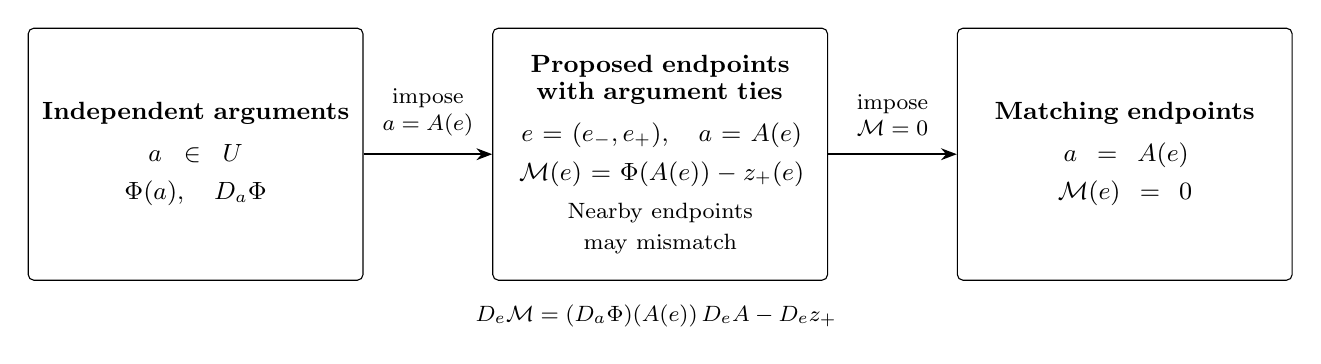
\begin{tikzpicture}[
  box/.style={draw, rounded corners=2pt, align=center,
    text width=3.9cm, minimum height=3.2cm, inner sep=5pt,
    font=\small},
  flow/.style={-{Stealth[length=2mm]}, thick},
  note/.style={font=\footnotesize, align=center}
]
\node[box] (ambient) at (0,0) {
  \textbf{Independent arguments}\\[4pt]
  $a\in U$\\[3pt]
  $\Phi(a),\quad D_a\Phi$
};
\node[box] (graph) at (5.9,0) {
  \textbf{Proposed endpoints}\\[-1pt]
  \textbf{with argument ties}\\[4pt]
  $e=(e_-,e_+),\quad a=A(e)$\\[3pt]
  $\mathcal M(e)=\Phi(A(e))-z_+(e)$\\[3pt]
  {\footnotesize Nearby endpoints may mismatch}
};
\node[box] (matched) at (11.8,0) {
  \textbf{Matching endpoints}\\[4pt]
  $a=A(e)$\\[3pt]
  $\mathcal M(e)=0$
};
\draw[flow] (ambient.east) -- node[note, above=3pt]
  {impose\\$a=A(e)$} (graph.west);
\draw[flow] (graph.east) -- node[note, above=3pt]
  {impose\\$\mathcal M=0$} (matched.west);
\node[note] at (5.9,-2.05) {
  $D_e\mathcal M=(D_a\Phi)(A(e))\,D_eA-D_ez_+$
};
\end{tikzpicture}
\caption{One link near an actual passage, with physical parameters fixed.
The arrows impose successive equations.  Regular argument ties express
all independent kernel arguments, including coefficient copies, in terms
of nearby proposed endpoints before the scalar transfer equation is
imposed.  Here $z_+(e)$ is the prescribed output coordinate in the chosen
traversal.  On this local tied graph, $\mathcal M$ is the physical mismatch
in regular transverse coordinates, including at mismatched pairs.
Ambient partial derivatives are taken in $a$; endpoint derivatives use
the displayed chain rule.  This is a local statement, not a claim that
every point of the extended matching domain is a physical passage.}
\label{fig:matching-arguments}
\end{figure}


\paragraph{The specified open domains.}
We list all domain restrictions as strict margins: positive clock
and root conditions; ordering; all nonzero divisors; coordinate-box
and smallness restrictions for bounded analytic arguments; coefficient
signs and ranges; and the state and rate margins ensuring that the
real transfer exists in its larger state disk.  The finite analytic
charts are chosen with a larger extension about their closed smaller
argument boxes.  The target smallness thresholds from the geometric
reduction are chosen strictly inside these boxes.

For additive transfers this includes $Q>q>q_*$ for the fixed large
threshold $q_*$, a sufficiently small $|\delta|$, and small layer
amplitudes and state inputs.  The action is increasing.  The real
estimates of Theorem~\ref{thm:additive-packets} give state room:
model (A) has damping and a small integral of the nonconstant-power
forcing; in model (B) the large $q_*$ makes the adverse fixed power
factors harmless in the integrals of the fast layers.  For mixed
transfers, fixed rate-sign margins, small amplitudes, and smaller
state boxes give the corresponding room from
Theorem~\ref{thm:mixed-packets}; stable orientation is used in the
damped model.  The regular and bounded-action alternatives use the
integrated bounds of Theorems~\ref{thm:regular-packets} and
\ref{thm:terminal-reduction}.  For example their small integrated
coefficients are explicitly tied arguments of the form $BL$,
$B\tau_e^\lambda$ on a long-length alternative, or
$LB\tau_e^\lambda$ on a short-length alternative.  Alternative
length ranges overlap about their cutoffs.  These finite conditions
are coordinate, polynomial/product, or bounded analytic inequalities,
with the same affine clock exponentials already allowed in the
argument graphs.

Thus a bounded sequence whose listed margins stay bounded away from
zero has a limit in the same boxes, sign and ordering domains, and
real existence regime.  Every formula is analytic at that limit and
the limit is admissible.  No additional condition that a long
mismatched arc remain in a physical subdivision cell is imposed.
The analytic systems are the normalized kernels on the stated
domains; their identification with physical motion is needed locally
at the target representations.  This distinction supplies exactly the
domain completeness required in Definition~\ref{def:counting-domain}.
It also remains valid after adding a determinant margin: a bounded
sequence with that margin bounded below cannot leave its minor
chart.

\paragraph{Local physical validity and rank.}
At a target representation and its fixed actual parameter value,
Lemma~\ref{lem:terminal-tied-endpoints} identifies each tied transfer
equation with a true scalar-flow endpoint mismatch, up to a regular
state coordinate and a nonzero factor.  The connector has the same
property by \eqref{eq:counting-connector}.  The subarcs are interior
and their clocks have nonzero velocity, so this identity holds for
all nearby proposed endpoints, not only for matching pairs.

One can see directly why a normalization chosen from the proposed
endpoint does not spoil the differential.  For a held normalization
$a$, let $H(e_-,e_+,a)$ be the transformed mismatch.  In local
coordinates consisting of a physical scalar mismatch $\Delta_0$
and the remaining variables, regularity gives
$H=U(e_-,e_+,a)\Delta_0$ with $U\ne0$.  This follows, for example,
by integrating $\partial_{\Delta_0}H$ from $0$ to $\Delta_0$.
After substituting $a=a(e_-,e_+)$, its differential on
$\Delta_0=0$ is still $U\,\dd\Delta_0$.
If the terminal clock is also transformed, its nonzero clock
velocity determines the hitting-time variation; the regular
coordinate pair leaves a nonzero transverse mismatch.  The exact
residual-amplitude identities displayed above and the weight-zero
invariance of the diagonal terms ensure the premise for all the
terminal transformations used here.

Choose local flow coordinates $(s_j,r_j)$ at the $k$ endpoints,
with $s_j$ tangential and $r_j$ transverse.  Up to nonzero row
factors, the link differentials at a matching cycle are
\begin{equation}\label{eq:counting-cyclic-rank}
 \dd r_{j+1}-h_j\,\dd r_j,
 \qquad j\in\ZZ/k\ZZ,
\end{equation}
where $h_j\ne0$ is the derivative of the corresponding section
holonomy.  Reversing the orientation used to write one link merely
changes this equivalent equation by a nonzero factor.  The kernel
of the cyclic transverse matrix satisfies
$\dd r_1=(\prod_j h_j)\dd r_1$.  For a hyperbolic orbit its return
multiplier is $\prod_j h_j\ne1$, so that kernel is zero and the
$k$ link rows have rank $k$.  The tangential variables remain free,
as intended.  Adding the auxiliary graph equations adds an
invertible block in their own variables.  Equivalently, eliminating
that block by row operations leaves exactly
\eqref{eq:counting-cyclic-rank}.  Hence the complete equation
Jacobian has full row rank, and at least one of its finitely many
maximal minors is nonzero.

For a word with $k$ links and $n_{\rm aux}$ auxiliary unknowns, the
fiber has $2k+n_{\rm aux}$ unknowns and $k+n_{\rm aux}$ equations.
Near a hyperbolic target its dimension is therefore $k$, accounted
for by the tangential positions of the cuts.  Hyperbolicity gives
full row rank of this matching system.  The following argument shows
that a connected component cannot contain targets from two different
cycles.

\paragraph{Injection into analytic components.}
Fix a word, its actual parameter tuple, and one nonzero-minor chart.
Let $M$ be a connected component of its analytic fiber and let
$E:M\longrightarrow\RR^2$ map a representation to its first
physical endpoint.  Suppose $M$ contains a target on a hyperbolic
cycle $C$.  In a neighborhood of that representation, exact local
matching and uniqueness of the nearby fixed point of the return
map imply $E\in C$.  The free tangential cuts only move points
along $C$.

We claim that $E(M)\subset C$.  The periodic trajectory $C$ is a
compact embedded nonsingular real analytic curve: it is analytic
by analytic ODE dependence, regular because $V$ has no zero on a
nonconstant periodic trajectory, and embedded by uniqueness and
use of a minimal period.  Put
$A=\operatorname{int}_M E^{-1}(C)$.  This is nonempty and open.
If $q\in\overline A$, closedness of $C$ gives $E(q)\in C$.
Near $E(q)$ a regular analytic defining function $h$ cuts out
exactly $C$.  Choose a connected analytic neighborhood $B$ of $q$
with $E(B)$ in that neighborhood.  The analytic function $h\circ E$
vanishes on the nonempty open set $A\cap B$, so the analytic
identity theorem makes it zero on $B$.  Thus $q\in A$; $A$ is
closed, and connectedness gives $A=M$.

Different periodic trajectories are disjoint by uniqueness of the
ODE.  They therefore cannot have target representations on the
same component $M$.  This argument permits remote points of $M$
that are not physical passage representations.  It uses physical
validity on the initial neighborhood and analytic continuation on
the entire component, which is precisely why no additional global
physical-cell restriction was imposed.

For each word we have now constructed a fixed open analytic system.
Its domains are positive-margin complete, every retained cycle has a
representation, and different hyperbolic cycles occupy different
components on each maximal-minor chart.  To apply the projection theorem,
it remains to prove absolute isolated-zero finiteness for every finite
system generated from these data.

\subsection{Absolute zeros of the matching systems}

Fix the matching systems just constructed, including their independent
kernel arguments, graph ties, and strict domain restrictions.  A system
in the counting closure may also contain derivatives, inverse margins,
and multiplier variables.  When its arguments approach a boundary, we
will rewrite its kernels by exact identities and retain every added
graph equation.  The next two lemmas state what these rewritings preserve;
the recovery lemma records the consequence used when a free flag input
is varied in the final contradiction.

\begin{lemma}[Graph and finite-jet lifting]\label{lem:counting-jet-lift}
Suppose an analytic transfer $\Phi(u)$, on an open set of its original
independent arguments $u$, has an exact analytic decomposition into
finitely many transfers, with auxiliary arguments and intermediate
states determined by regular, locally unique graph equations.  A
finite system involving $\Phi$ and finitely many of its independent
derivatives can be replaced, locally at any admissible tuple, by a
system involving those transfers and finitely many of their
derivatives.  The replacement, with the graph equations retained,
is locally analytically isomorphic to the original solution set.
In particular it preserves isolated solutions.  This conclusion also
holds along a sequence with shrinking graph neighborhoods, provided
one fixed finite decomposition is used along the sequence.
\end{lemma}

\begin{proof}
If $G(u,v)=0$ has $G_v$ invertible, its selected solution is a
locally unique analytic graph $v=v(u)$.  Projection of that graph to
$u$ is an analytic isomorphism.  Substituting $v(u)$ in any other
equations proves the first assertion about their solution sets.
Denominator clearing preserves this assertion on the retained
nonzero domain.

For the derivative assertion, differentiate the identity expressing
$\Phi$ in terms of the other transfers \emph{after} their arguments
have been put on their graphs.  Implicit derivatives of $v(u)$ are
obtained successively from $G_v^{-1}$ and finite derivatives of $G$.
The finite chain rule expresses each requested derivative of $\Phi$
using only finitely many such quantities.  They may either be
substituted, or be given their own graph coordinates.  In the latter
description, the equations for derivatives of order $j$ are linear
with coefficient $G_v$ in the order-$j$ unknowns and have previously
determined lower-order terms.  Their complete finite-jet Jacobian is
block triangular with invertible diagonal.

In particular, for a subdivision into $K$ consecutive subflows,
write
\[
 z_j=\Phi_j(a_j(u),z_{j-1}),\qquad 1\le j<K,
 \qquad
 \Phi(u)=\Phi_K(a_K(u),z_{K-1}).
\]
The intermediate-state equations have a triangular Jacobian with
unit diagonal.  If jets are adjoined, each derivative of $z_j$ is
determined from the earlier $z_i$ and their jets; these graph equations
again have unit diagonal.  Thus the augmented system has precisely
the original germ of solutions and no additional local degree of
freedom.  This is a pointwise assertion at each member of a sequence;
no uniform radius of the isomorphism is needed to preserve isolation.
\end{proof}

Two consequences will be used below.  First, partial derivatives of
two independently enlarged kernels cannot be identified just because
their values agree on a graph.  Only the differentiated composition
identity in Lemma~\ref{lem:counting-jet-lift} is used.  Second, a
finite $K$ chosen after taking a subsequence is legitimate in an
absolute zero contradiction: it produces one fixed finite system for
that sequence.  It does not assert a degree-uniform value of $K$ and
does not add links to the geometric word count.

\begin{lemma}[Cleared finite differential closure]
\label{lem:counting-cleared-closure}
Consider one fixed finite collection of primitive functions, their
argument graphs, and a finite differential and algebraic construction
from them.  Assume that, after one fixed exact graph enlargement, the
primitive functions and defining graph equations extend analytically
near a finite limiting tuple.  The selected graph Jacobians and every
declared divisor need be nonzero only at the points of the sequence,
not at its limit.  Then the constructed equations can be replaced by
analytic equations near that limit, retaining all graph equations and
all original open restrictions, with exactly the same solution germ
at each selected point.  Additional multiplier coordinates, polynomial
equations, and parameter copies or specializations preserve this
assertion.
\end{lemma}

\begin{proof}
First differentiate every exact rewriting as an identity on its old
open argument domain.  For a graph $G(u,v(u))=0$ this gives
\[
 v_{u_i}=-G_v^{-1}G_{u_i}.
\]
Cramer's rule and induction on derivative order express every requested
implicit derivative as a quotient of polynomials in finite jets of
$G$, with denominator a power of $\det G_v$.  The same argument
applies successively to a finite stack of graphs and to the finite
composition identities in Lemma~\ref{lem:counting-jet-lift}.

Every further algebraic or differential operation preserves a rational
expression in a finite collection of analytic jets.  For example,
\[
 \partial_i(A/B)
   =\frac{B\partial_iA-A\partial_iB}{B^2},
 \qquad (A/B)^{-1}=B/A
\]
on the retained nonzero domains.  An inverse of a new expression
therefore adds its nonzero numerator to the possible denominator
factors; a determinant is a polynomial in its entries.  Thus each
final equation is $A/B=0$, where $A,B$ are analytic near the limiting
tuple and $B$ is nonzero at every selected point.  Replacing it by
$A=0$ leaves its solution germ unchanged there.  This replacement
does not require a bound on $B^{-1}$, nor does it append its value
as a new coordinate.  In particular a margin or a graph determinant
tending to zero causes no difficulty at this step.  Finite jet
coordinates, if retained instead of substituted, have the
differentiated analytic graph equations of
Lemma~\ref{lem:counting-jet-lift}; their Jacobians need be invertible
only at the selected points.

New multipliers are coordinate factors in these expressions.  A
parameter copy has a polynomial equation $p'-p=0$, and a fixed
specialization has an equation $p-p_0=0$.  Unrestricted added
coordinates likewise enter the closure through polynomial and
rational operations.  These operations introduce no new primitive
function or evaluation outside its original argument domain.  Their
finite derivatives are of the same form, proving the last assertion.
\end{proof}

\begin{lemma}[Recovery after graph enlargement]
\label{lem:counting-graph-recovery}
Let $u_i$ be a sequence of isolated solutions of a fixed system,
where $u$ denotes its full tuple, including parameters and multipliers.
Suppose an exact finite enlargement appends $v_i$ by equations
$G(u,v)=0$ whose selected graph Jacobian $G_v(u_i,v_i)$ is invertible
at every point.  Retain all these equations.  An old flag input
recoverable from $(u,v)$ cannot vary along the local lifted solution
set while $u$ stays fixed, provided the variation is taken within the
selected graph neighborhood.  These neighborhoods may shrink
arbitrarily along the sequence.
\end{lemma}

\begin{proof}
At each $i$ the implicit function theorem supplies an open neighborhood
$N_i$ in which $v=g_i(u)$ is the unique selected solution of the
complete graph equations.  Let $B_i$ be any proposed isolation
neighborhood of $u_i$.  Intersect $N_i\cap\pi^{-1}(B_i)$, where
$\pi(u,v)=u$, with the local real flag chart and all strict domain
neighborhoods at that point.  This is an open neighborhood of the
lifted point.  By continuity of the chart map, all sufficiently small
variations of a free chart input remain in it.  The size is chosen
separately for every $i$; it can also be made small enough to preserve
the prescribed comparisons and ordinary limits for the retest in
Theorem~\ref{thm:absolute-zero}.

Write $S_*=R(u,v)$ for the retained old free input, recovered by the
locally invertible affine and lifted logarithmic flag changes.
For any such varied solution, $u'=u_i$ would imply
$v'=g_i(u_i)=v_i$ and hence $S_*'=S_*$, a contradiction if this
input was changed.  Thus a nonzero sufficiently small permitted
variation gives a different original tuple inside $B_i$.  Vanishing
graph determinants at the limiting tuple affect only the sizes of
the individual neighborhoods, not this argument.
\end{proof}

\begin{proof}[Completion of the proof of Theorem~\ref{thm:matching-system}]
Fix an arbitrary finite system in the closure required by
Theorem~\ref{thm:projection-count}, including its equations and every
original graph and strict domain restriction.  Suppose it has a
sequence of distinct isolated total solutions.  Multipliers and
coordinates formerly called parameters are now ordinary unknowns.
Clear all declared nonzero denominators, retaining their restrictions.
Only finitely many derivatives of finitely many transfer kernels,
argument graphs, and margins occur, together with algebraic factors
in the coordinates.
This assertion is hereditary under the projection construction:
gradients of inverse margins, products with new multiplier coordinates,
and determinants of their derivatives have exactly this form by
Lemma~\ref{lem:counting-cleared-closure}.  Parameter copies and
specializations add polynomial equalities.  Thus an unbounded new
coordinate is included in the large-coordinate analysis below, while
a bounded new coordinate is just an additional ordinary argument of
these polynomial expressions.  No new transfer family is introduced.

At every transfer choose a subsequence regime of
Theorem~\ref{thm:terminal-reduction}; there are finitely many transfers
in this fixed system.  Append any bounded ratios or auxiliary
coordinates required by that regime by their unique regular graph
ties.  For example, the bounded-ratio additive corner is normalized
by
\begin{equation}\label{eq:counting-ratio}
 S=Q-q,\qquad M=S/q,\qquad
 y+\delta\log y=1+Ms.
\end{equation}
If $M$ tends to a finite value, a fixed sufficiently large finite
subdivision into $K$ fractions gives regular analytic normalized
pieces.  The value of $K$ is chosen once for this limiting corner.
Its internal states and amplitudes are regular graphs.  Internal
amplitudes are products of bounded positive ratios and exponentials
of fixed affine clock fractions; for instance a left additive layer
at fraction $j/K$ has amplitude
\[
 e_j=e\,(w_j/q)^\beta e^{-a jS/K}.
\]
The real layer estimates keep these amplitudes in the permitted
boxes.  The mixed unbalanced auxiliary ratio $C_{\rm aux}=P/R$ is
also appended where required by the mixed packet construction; here
$P,R$ denote that construction's positive scales, not the components
of the polynomial vector field.

All derivatives of the original kernel are obtained by differentiating
the exact identities on its original open argument domain.  For
example if the decomposition in \eqref{eq:counting-ratio} reads
$\Phi(Q,q,\delta,a)=\Psi(S,M,\delta,a)$, then
\[
 \Phi_Q=\Psi_S+q^{-1}\Psi_M,
 \qquad
 \Phi_q=-\Psi_S-(Q/q^2)\Psi_M.
\]
Higher derivatives use finitely many rational factors and kernel
derivatives, with the same nonzero denominators.  The other bounded
clock and subdivision identities are handled by the same chain rule,
as proved in Lemma~\ref{lem:terminal-ambient-extension}.
Lemma~\ref{lem:counting-jet-lift} therefore lifts the isolated
solutions, including any equations containing derivatives, to
isolated solutions of one fixed finite enlarged system.  Using a
different $K$ at every term of the sequence would not give this
conclusion; the fixed finite choice just described does.

\paragraph{Bounded enlarged tuples.}
Suppose first that every coordinate of the enlarged tuple remains
bounded, and pass to a finite limit.  Some strict margins may vanish.
Positive-margin domain completeness, used for the proper barrier,
does not prove analytic extension at such a limit.
Lemma~\ref{lem:terminal-boundary-corners} instead gives the required
extension of each \emph{old independent-argument} normalized kernel:
closed smaller argument and amplitude boxes lie within larger analytic
boxes, and the integrated-field bounds leave a positive state margin
on their closures.  The bounds use independent coefficient copies,
before any physical slope or normalization ties are imposed.  At a
bounded clock corner these normalized fields therefore define analytic
transfers near the limiting data, including when a clock is zero.

For example, the normalized mixed equations have the forms
\[
 v_s=-Wv+L g(X,Y,v),\qquad z_s=L G(X,Y,z),
\]
with layer exponents $\alpha L+\beta W$ and other coefficient copies
retained independently.  They contain no singular $W/L$ in these
positions and are analytic also at $(L,W)=(0,0)$.  A slope needed
elsewhere is its own coordinate, tied by $L c-W=0$.  If it stays
bounded, this polynomial graph is analytic at the corner.  If a
necessary new ratio diverges, the enlarged tuple has a large coordinate
and belongs to the large-coordinate case below; boundedness of the
\emph{old} tuple alone is not the criterion for the present case.

The remaining possible degenerations of the endpoint graphs are
equally explicit.  A ratio has an equation $bv-a=0$.  A positive
rational root has an equation $u^B-q^A=0$, made polynomial by
clearing negative powers when necessary.  Clock and residual ties have
the forms
\[
 t_- -t_+e^{-L}=0,
 \qquad R_+-R_-e^{\kappa S+z_+}=0.
\]
They extend analytically when all their coordinates remain finite,
even if their derivatives in $L$ or $z_+$ tend to zero with the
positive endpoints.  If $t_+/t_-\to\infty$, then
$L\to\infty$, which is a large-coordinate case.  Connector
coefficients have polynomial graph equations after multiplication by
$V_X(X_-,Y_-)$ and $r$, and $r^2=\Delta$ is polynomial.  Their
bounded normalized coefficient arguments remain in the larger
analytic connector box when either divisor tends to zero.
Regular endpoint inversions may likewise retain their analytic
defining equations.  Their graph Jacobians need only be nonzero at
the selected points.  Finite implicit derivatives then have exactly
the denominator description of
Lemma~\ref{lem:counting-cleared-closure}.

Consequently all primitive transfers and defining graph equations
extend analytically at the finite limiting tuple of the enlarged
system.  That lemma clears
the finite derivative and multiplier equations without asserting
invertibility of a limiting graph Jacobian.  Only equations are
cleared; no inequality is replaced by an unverified numerator sign.
The old strict inequalities and all later determinant restrictions
remain as open restrictions at each selected point.  Their limiting
values may vanish, and their differentiated forms need not themselves
extend across that boundary.  This is sufficient here, in contrast
to the positive-margin completeness used in the projection theorem.
Local finiteness of components
of a real analytic set excludes an accumulating sequence of its
isolated zeros \cite[Corollary~2.7]{BierstoneMilman1988}.
Each point of the original strict domain is interior to that domain,
so it cannot become an isolated zero merely by intersecting a
nonisolated germ with those open restrictions.  This excludes the sequence of isolated solutions when its enlarged
tuple has a finite limit.

\paragraph{Divergent enlarged tuples.}
Suppose instead that at least one enlarged coordinate diverges.
Split all coordinates of the enlarged sequence into bounded
convergent coordinates and signed large coordinates.  Apply the
affine flag construction of Section~\ref{sec:flags} to the latter,
keeping bounded remainders as ordinary coordinates.  Convert the
initial basis scales, including scales used in polynomial factors,
to dependent logarithmic nodes, and insert the further logarithms
required by the primitive constructions.  Saturate the resulting
finite flag.  These real coordinate changes are locally invertible.
The kernel rates are affine in the primary clock coordinates and
bounded remainders.  Polynomial powers of the initial scales are
now shift monomials times bounded analytic factors.  Under an
inserted logarithm, old independent derivatives become finite sums
of packet independent derivatives multiplied by constants, signs,
and reciprocal powers of the logged dependent scale.  These are
precisely operations of Theorem~\ref{thm:calculus}.
If only a multiplier or an algebraic auxiliary coordinate diverges
while a kernel's clocks remain bounded, that kernel keeps its
ordinary analytic normalized formula.  It is a packet constant in
the extra free inputs before pullback; the new polynomial coordinate
factors are treated by the preceding logarithmic conversion.  In
particular a large auxiliary ratio at bounded primary clocks does
not invoke an unbalanced mixed theorem that requires both clocks
large.

Theorem~\ref{thm:terminal-reduction}, with the differentiated packet
theorems, supplies the packet data for this finite derivative
request on independent flag inputs.  Graph ties remain equations;
they are not assumed to hold when taking independent tests of a
primitive kernel.  In particular a bounded coefficient copy and a
clock ratio remain separate arguments until their graph identity is
used by the chain rule.  The layer-vanishing residual extensions of
Lemma~\ref{lem:terminal-ambient-extension} are essential here.
For each nonzero equation, iterated left-finiteness permits a leading
shift normalization making both sign trees nonnegative in the series
sense.  A formally zero equation is handled by separation.  All
normalizing monomials are nonzero on the real domain and use the
current flag backgrounds.  The finitely many real normalized
equations can then be combined by a sum of squares, exactly as in
Theorem~\ref{thm:absolute-zero}; the resulting positive operations
are covered by Theorem~\ref{thm:calculus}.

\paragraph{Retesting and return to the original solutions.}
We verify the retestability of this assembled library in the precise
sense of Definition~\ref{def:elimination-retestable}.  For the
primitive transfers this is the coefficient-germ assertion of
Theorems~\ref{thm:additive-packets}, \ref{thm:regular-packets}, and
\ref{thm:mixed-packets}, carried through the exact terminal identities
by Theorem~\ref{thm:terminal-reduction}.  The affine and logarithmic
flag identities, fixed analytic fields, sector signs, and ordinary germs
are unchanged by sufficiently small absolute perturbations preserving
the selected comparisons.  Terminal coefficients are the fixed
formal recursions and, where an infinite anchor is used, its fixed
normalized jets.  Cutoff and finite-anchor choices have already
dispersed before these terminal leaves are taken.  Subsequent
algebra and finite derivatives preserve those same defining germ
identities.  The implicit inversion of
Theorem~\ref{thm:calculus} is used only when the limiting
exponent-zero Jacobian is invertible.  A root, logarithmic, or ratio
graph that is regular at every selected point but degenerates at the
limit is instead retained as an equation in its own coordinates;
it is not inverted by the packet implicit theorem.  Its finitely
many old-coordinate derivatives are expressed by Cramer's rule and
their nonzero denominators are cleared, leaving finite algebraic
expressions in independent jets of the defining equations.  At
large scales these equations use the already admitted affine shifts
and bounded analytic fields.  The ordinary elimination theorem
then treats them together with all the other equations, including
any multiple limiting zero.  Thus only actual unit-Jacobian
ordinary chart operations invoke the implicit part of
Theorem~\ref{thm:calculus}; no packet inverse at a degenerate
limiting graph is assumed.  Further flag refinements leave the old
free inputs free.  At least one such input is recoverable from the
tuple before the flag changes whenever a large scale remains.  The
sequence-wise graph enlargement retained all its defining equations,
so Lemma~\ref{lem:counting-graph-recovery} makes it recoverable for
the original isolation test as well.  More explicitly, at each
anchor choose the free variation inside that anchor's graph-uniqueness
neighborhood, the real flag chart, and the pullback of the proposed
original isolation neighborhood.  Such variations may be chosen
arbitrarily small, with no common radius required along the sequence.
All the hypotheses of
Theorem~\ref{thm:absolute-zero} therefore hold.  It excludes the
isolated sequence in that case; the small free variations used there
can be made inside every strict open condition at the selected
point.

The two alternatives prove the absolute zero property for the arbitrary
finite system under consideration.  All additional determinant margins
and multiplier systems use the same finite operations, so the conclusion
holds for them as well.

Together with the construction and geometric arguments above, this
proves all three assertions of Theorem~\ref{thm:matching-system}, including
the assertion about maximal-minor charts.
\end{proof}

\subsection{Rotation and the bound in the whole plane}

\begin{lemma}[Hyperbolic realization of a finite cycle count]
\label{lem:counting-rotation}
For any finite collection of limit cycles of a planar polynomial
field $V=(P,Q)$, a sufficiently small perturbation
$V_\mu=V+\mu(-Q,P)$, of one common nonzero sign, has at least as
many distinct hyperbolic periodic orbits in the union of disjoint
neighborhoods of that collection.  The degree bound is preserved.
\end{lemma}

\begin{proof}
Let $z(t)$ parametrize one selected cycle with period $T$, and start
the perturbed solution at the same section point.  Set
$u(t)=\partial_\mu z_\mu(t)|_{\mu=0}$ and
$J(a,b)=(-b,a)$.  Then
\[
 u'=DV(z(t))u+JV(z(t)),\qquad u(0)=0.
\]
For $w(t)=\det(V(z(t)),u(t))$, the identity
$\det(Aa,b)+\det(a,Ab)=\operatorname{tr}(A)\det(a,b)$ gives
\begin{equation}\label{eq:counting-rotation}
 w'=(\operatorname{div}V)(z(t))w+|V(z(t))|^2,
 \qquad
 w(T)=\int_0^T
 e^{\int_s^T(\operatorname{div}V)(z(\tau))\,\dd\tau}
 |V(z(s))|^2\,\dd s>0.
\end{equation}
The return-time correction adds a multiple of $V$ to the terminal
variation and does not change this determinant.  Thus the local
analytic Poincare displacement $D(r,\mu)$ has
$D_\mu(0,0)\ne0$ in a transverse section coordinate $r$ centered
at the cycle.

The analytic implicit function theorem writes its zero set as
$\mu=\psi(r)$ near $(0,0)$, with $\psi(0)=0$.  Isolation of the
cycle makes $D(r,0)$ a nonzero analytic germ, so
\[
 \psi(r)=a r^m+O(r^{m+1}),\qquad a\ne0,\quad m\ge1.
\]
For odd $m$, both sufficiently small signs of $\mu$ give one
nearby nonzero root; for even $m$, the sign of $a$ gives two.
All these roots are simple because
$\psi'(r)=ma r^{m-1}+O(r^m)\ne0$ for sufficiently small
$r\ne0$.  Differentiating $D(r,\psi(r))=0$ then gives
$D_r=-D_\mu\psi'\ne0$ at these roots.  A planar return map has
positive derivative (as follows from its scalar variational
equation), so a simple fixed point has multiplier different from
$1$ and is hyperbolic.

Choose disjoint tubular neighborhoods of the finitely many original
cycles and one common sufficiently small magnitude of $\mu$.
If $O$ cycles have odd order and $E_+$ and $E_-$ have even order
favoring the two signs, the resulting numbers are at least
$O+2E_+$ and $O+2E_-$.  Their maximum is at least
$O+E_++E_-$, the original selection size.  The count is taken over
the union: an even-order cycle favoring the other sign need not
persist for the chosen rotation.  The new cycles are
distinct because their neighborhoods are disjoint (and the two
roots in one sufficiently small return section give different
periodic orbits).  Finally $V_\mu$ is obtained by constant linear
combinations of $P,Q$, and still has degree at most $d$.
\end{proof}

\begin{proof}[Proof of Theorem~\ref{thm:uniform}]
Fix $d$.  For every word $w$ of Theorem~\ref{thm:matching-system}
and every one of its maximal-minor charts $I$, apply
Theorem~\ref{thm:projection-count}.  Let $N_{w,I}<\infty$ be the
resulting component bound.  It is independent of the numerical
value of every polynomial coefficient and preparation parameter.
The component injection gives, in the fixed square, the uniform
bound
\begin{equation}\label{eq:counting-final-bound}
 B_*(d)=T(d)+\sum_{w\in\mathcal W_d}\ \sum_I N_{w,I}
\end{equation}
for hyperbolic periodic orbits.  An orbit represented in more than
one chart is assigned to any one of them; overcounting in this sum
is harmless.  Finiteness of the sums is geometric template
finiteness, and does not involve the internal $K$ used in a
sequence-dependent absolute zero test.

Now select any finite collection of limit cycles of any field of
degree at most $d$ in the whole plane.  A spatial affine scaling
$z=a+Ru$, $R>0$, puts all of them strictly inside the fixed square.
The transformed field is
$\dot u=R^{-1}V(a+Ru)$, again polynomial of degree at most $d$;
isolation and geometric distinctness are preserved.  Apply
Lemma~\ref{lem:counting-rotation} there.  The perturbation can be
chosen small enough that its retained hyperbolic cycles remain in
the square.  Their number is at least the size of the selected
collection and is at most $B_*(d)$ by
\eqref{eq:counting-final-bound}.  Hence every finite collection has
size at most $B_*(d)$.  If the original field had more limit cycles,
one could select $B_*(d)+1$ of them, a contradiction.  Taking any
integer upper bound for $B_*(d)$ defines the required finite
$B(d)$, without an assumption of prior individual finiteness.
\end{proof}

\bibliographystyle{plainnat}
\bibliography{references/references}
\end{document}
